% TMLR submission. Built 10 November 2026 from:
%   paper/00_PROSE_v1.md   the author's written sections, 78 figures auto-verified
%   report/REPORT_V2.md    the sprint report, every number recomputed by report/verify_v2.py
%
% ANONYMITY. \usepackage{tmlr} with no option is the anonymous submission mode: the tmlr
% package hides the author block itself. Switching to [preprint] de-anonymises for arXiv AND
% turns on the \ifpreprint branches below, which are the only places a name, a repository URL
% or the benchmark's distinctive name appears. So one source produces both documents and the
% anonymous build cannot leak an identifier that the preprint build adds.
%
% Build:  latexmk -pdf main.tex
\documentclass[10pt]{article}

% The mode is chosen at build time so that one source produces every variant and they cannot
% drift apart:
%   latexmk -pdf main.tex                                        anonymous TMLR submission
%   pdflatex "\def\TMLRMODE{preprint}% TMLR submission. Built 10 November 2026 from:
%   paper/00_PROSE_v1.md   the author's written sections, 78 figures auto-verified
%   report/REPORT_V2.md    the sprint report, every number recomputed by report/verify_v2.py
%
% ANONYMITY. \usepackage{tmlr} with no option is the anonymous submission mode: the tmlr
% package hides the author block itself. Switching to [preprint] de-anonymises for arXiv AND
% turns on the \ifpreprint branches below, which are the only places a name, a repository URL
% or the benchmark's distinctive name appears. So one source produces both documents and the
% anonymous build cannot leak an identifier that the preprint build adds.
%
% Build:  latexmk -pdf main.tex
\documentclass[10pt]{article}

% The mode is chosen at build time so that one source produces every variant and they cannot
% drift apart:
%   latexmk -pdf main.tex                                        anonymous TMLR submission
%   pdflatex "\def\TMLRMODE{preprint}% TMLR submission. Built 10 November 2026 from:
%   paper/00_PROSE_v1.md   the author's written sections, 78 figures auto-verified
%   report/REPORT_V2.md    the sprint report, every number recomputed by report/verify_v2.py
%
% ANONYMITY. \usepackage{tmlr} with no option is the anonymous submission mode: the tmlr
% package hides the author block itself. Switching to [preprint] de-anonymises for arXiv AND
% turns on the \ifpreprint branches below, which are the only places a name, a repository URL
% or the benchmark's distinctive name appears. So one source produces both documents and the
% anonymous build cannot leak an identifier that the preprint build adds.
%
% Build:  latexmk -pdf main.tex
\documentclass[10pt]{article}

% The mode is chosen at build time so that one source produces every variant and they cannot
% drift apart:
%   latexmk -pdf main.tex                                        anonymous TMLR submission
%   pdflatex "\def\TMLRMODE{preprint}% TMLR submission. Built 10 November 2026 from:
%   paper/00_PROSE_v1.md   the author's written sections, 78 figures auto-verified
%   report/REPORT_V2.md    the sprint report, every number recomputed by report/verify_v2.py
%
% ANONYMITY. \usepackage{tmlr} with no option is the anonymous submission mode: the tmlr
% package hides the author block itself. Switching to [preprint] de-anonymises for arXiv AND
% turns on the \ifpreprint branches below, which are the only places a name, a repository URL
% or the benchmark's distinctive name appears. So one source produces both documents and the
% anonymous build cannot leak an identifier that the preprint build adds.
%
% Build:  latexmk -pdf main.tex
\documentclass[10pt]{article}

% The mode is chosen at build time so that one source produces every variant and they cannot
% drift apart:
%   latexmk -pdf main.tex                                        anonymous TMLR submission
%   pdflatex "\def\TMLRMODE{preprint}\input{main}"               de-anonymised arXiv preprint
%   pdflatex "\def\TMLRMODE{accepted}\input{main}"               camera-ready
% Use build.py, which runs all of them and checks the anonymous output for leaks.
\providecommand{\TMLRMODE}{submission}
\makeatletter
\def\@tmlrpreprint{preprint}
\def\@tmlraccepted{accepted}
\ifx\TMLRMODE\@tmlrpreprint
  \usepackage[preprint]{tmlr}
\else
  \ifx\TMLRMODE\@tmlraccepted
    \usepackage[accepted]{tmlr}
  \else
    \usepackage{tmlr}
  \fi
\fi
\makeatother

\usepackage{hyperref}
\usepackage{url}
\usepackage{booktabs}
\usepackage{graphicx}
\usepackage{amsmath}

% Gate every identifying string on whether identity may be revealed at all. The flag to test is
% \if@accepted, NOT \if@preprint: tmlr.sty's [preprint] option sets BOTH, so \if@accepted is true
% for the preprint and the camera-ready and false only for the anonymous submission, which is
% exactly the condition wanted. Gating on \if@preprint alone also hid the repository URLs from the
% camera-ready, which is where this paper promises to give them. \if@accepted is internal to
% tmlr.sty, hence the \makeatletter. The anonymous build takes the second argument.
\makeatletter
\newcommand{\ifdeanon}[2]{\if@accepted#1\else#2\fi}
\makeatother
\newcommand{\benchname}{\ifdeanon{SwarmInfluence-Bench}{the benchmark}}

% An unmarked footnote, for the LLM-use disclosure. TMLR's FAQ requires the disclosure and names
% the location: authors must "mention explicitly in their submission that they have used this
% tool", "as a footnote on the first page". Verified against jmlr.org/tmlr/faq.html on 10 Nov 2026.
% It is therefore not optional, and it does not belong in Broader Impact, where it sat until now.
% Nothing in the policy asks for the vendor's name, so none is given.
\newcommand{\disclosurefootnote}[1]{%
  \begingroup\renewcommand\thefootnote{}\footnote{#1}\addtocounter{footnote}{-1}\endgroup}

\title{An Influence Graph Over AI Agents Certifies an Agent That Copies Nobody}

% Hidden by the tmlr package unless [accepted] or [preprint] is given.
\author{\name Manu Nicholas Jacob \email manunicholasjacob@gmail.com \\
        \addr Independent Researcher}

\def\month{11}
\def\year{2026}
\def\openreview{\url{https://openreview.net/forum?id=XXXXXXXXXX}}

\begin{document}
\maketitle

\begin{abstract}
Circular-shift surrogates can produce severely inflated false-positive rates when applied to
turn-ordered multi-agent conversations, reaching a family-wise error rate of 0.90 against a nominal
0.05. A generated benchmark separates two candidate mechanisms and points at non-stationary speaker
activity rather than turn-taking, which suppresses the failure rather than causing it. No setting of
either knob reproduces the observed 0.90, however, so what drives the full real-data failure remains
open. Restricted permutation surrogates substantially reduce the problem. Their error rate is flat
with respect to drift rather than at the nominal level, and for the global within-speaker variant it
depends on how many surrogate draws the null is built from. Calibration alone does not address
confounding, which motivates a conditional estimator validated against a benchmark with planted
ground truth. I also identify a symbolisation-dependent detection limit and develop label-free
diagnostics for it, and show that their calibration does not transport across degradation
mechanisms. The benchmark is released.
\end{abstract}

\disclosurefootnote{\textbf{Use of a large language model.} A large language model was used as an
assistive tool: to help write and run the analysis code, and to help draft this paper. The author is
responsible for every claim, number and figure. All results come from the released code run on the
public dataset, no result or reference is fabricated, and every number in this paper is recomputed
from committed analysis output by a verifier that fails the build on a mismatch.}

\section{Introduction}

When AI agents interact in a shared channel, it is useful to understand how they influence one
another. Information-theoretic methods offer a way to measure this through lagged transfer entropy,
surrogate testing, and per-agent influence scores. They are attractive because they require no
labels and no access to model internals, only a record of who said what and when. The reliability of
those measurements is what this paper examines.

Almost every demonstration of these detectors runs on synthetic traces with a planted leader, where
the analyst controls timing and vocabulary. Real agent chat is asynchronous, bursty, and written in
open language. The narrower question here is whether the standard recipe, applied to real agent
logs, returns anything an overseer should act on.

The audit runs on the AI Village corpus \citep{aidigest2026}, in which frontier models share chat
channels over eighteen months across four villages differing in size, lifetime and tempo, applying
the checks a reader should demand: planted controls, a meaning-free symboliser, replication in a
held-out window, and sensitivity to every parameter that had to be chosen.

\begin{enumerate}
\item The conventional circular-shift surrogate is \textbf{invalid} on turn-ordered agent chat: a
family-wise error rate of 0.90 against a nominal 0.05, caused by the structure of the speaker
sequence itself.
\item Restricted permutation surrogates restore most of the calibration, and re-certifying under one
\textbf{scrambles rather than shrinks} the answer: one channel loses all 11 of its edges, another
gains 15.
\item The three restricted variants are \textbf{mutually indistinguishable} at the precision reached
here, so the choice between them cannot be justified on error rate. The global within-speaker
variant additionally needs on the order of 200 surrogate draws, and over-fires by roughly a factor
of two at 100.
\item Calibration is not confounding, so a conditional estimate is added and validated on a released
benchmark with a known influence graph: common-cause false edges fall from 22.3 to 0.33, and on the
planted-edge instances precision rises from 0.17 to 0.80 with no loss of recall or power.
\item The same benchmark exposes a \textbf{symbolisation floor}. Below roughly 0.44 adjusted Rand
index between symboliser and truth, detection collapses whatever the estimator. Label-free
diagnostics detect that floor, but their calibration does not transport across degradation
mechanisms, and I report where it fails.
\item On the real channels two edges stand at every conditioning resolution, 18 are
\textbf{undetermined} between 0 and 13, none replicates out of sample, and what survives alongside
humans runs from people to agents.
\end{enumerate}

\section{Related work}

\paragraph{Transfer entropy and surrogates.} Transfer entropy \citep{schreiber2000} measures how much
a source's past reduces uncertainty about a target's next symbol beyond the target's own past.
Plug-in estimators are biased upward on short series, so significance rests on surrogate data, with
family-wise error controlled by a max-T test \citep{westfall1993}. The usual surrogate is a circular
time shift of the source.

\paragraph{Event-based data breaks the shift surrogate.} \citet{shorten2021}, on neural spike trains,
show that the conventional source-time-shift surrogate fails to represent the null hypothesis of
conditional independence for event-based processes, and adapt to that setting the nearest-neighbour
local permutation scheme of \citet{runge2018}. Agent chat is event-based in that sense: messages are
events in continuous time, not samples of a clocked signal. The correction is not a contribution of
this paper. The contribution is showing that the same failure carries over to multi-agent safety
monitoring, and that it can be severe enough to create apparent leaders where none exist.

\paragraph{The same failure, concurrently, in multi-agent reinforcement learning.}
\citet{papadopoulos2026} report a closely related surrogate failure in multi-agent
reinforcement-learning action series. Their agent pairs have zero influence by construction, yet
circular time shifts produce false-positive rates of 100\% and 98.2\% against a nominal 0.05. A
plain permutation surrogate fares no better in their setting, at 100.00\% and 99.95\%. Their
proposed correction restricts permutations to blocks of training time, which returns the rates to
5.25\% and 5.50\%.

There are important differences between their setting and this one. Their data consist of binary
actions recorded over twelve thousand training rounds, whereas these data are symbolised
natural-language messages arranged on a turn-ordered conversational grid. Their non-stationarity
comes from monotone drift associated with annealing exploration; here the relevant non-stationarity
appears in the speaker sequence. Neither result should be taken as a direct extension of the other.

Nevertheless, the fact that both approaches rely on restricted permutations is worth noting. Their
permutation blocks are defined by training time, while mine are defined by an agent's own speaking
positions. This provides convergent evidence that unrestricted temporal rearrangement can be
problematic in non-stationary multi-agent data. Their findings also serve as a useful warning for
the approach taken here, and the warning has a measured form rather than a rhetorical one: in their
data the unrestricted permutation failed as completely as the time shift, at 100.00\% against a
nominal 0.05. Permutation-based surrogates are not automatically protected against
non-stationarity, and what protects the one used here is the restriction, not the permutation. I
claim no priority over their result and view the two studies as complementary, addressing different
forms of structured multi-agent data.

\paragraph{Oversight under a budget.} AI-control research frames monitoring as resource constrained,
with a cost for false positives \citep{greenblatt2024}. An influence graph is one such measurement,
and its error rate is the concern here.

\paragraph{Clustering stability.} The idea of using clustering stability as a label-free quality
indicator is not new. It has a substantial history, including \citet{benhur2002},
\citet{lange2004}, von Luxburg's review of clustering stability \citep{vonluxburg2010}, and
\citet{tibshirani2005} on prediction strength. What is different in Section~\ref{sec:floor} is the
calibration of these diagnostics against a detection-performance floor rather than against cluster
recovery alone.

\section{Data and representation}

The AI Village dataset ships one gzipped-JSONL table per village. Four villages are used, differing
enough to test whether any finding is a property of one channel.

\begin{table}[h]
\centering
\begin{tabular}{lrrrrl}
\toprule
village & agent messages & agents & lifetime & human messages & busiest room \\
\midrule
main      & 205,726 & 58  & 576 days & 10,029 & \#general (166,715, 81\%) \\
open-chat &  35,483 & 23  &  66 days & 12,264 & \#general (all) \\
swarm     &   3,848 & 133 &   1 day  &      5 & room a (3,846) \\
game-jam  &     838 & 6   &   3 days &     36 & per-team rooms \\
\bottomrule
\end{tabular}
\caption{The four villages. A 2026 scaffolding change scopes each agent to its current room's
context, so the busiest room of each village is a self-contained influence substrate and is analysed
alone.}
\end{table}

The primary window is the final fourteen days of main-village \#general, 17 to 31 October 2026,
holding 8,800 agent messages. Twenty-two models posted at least 50 messages each and the directed
test uses the 15 busiest, giving 7,958 message events. Two scaffolding facts are disclosed rather
than corrected: the automated nudger was off throughout, and the unused \#best and \#rest rooms were
soft-deleted mid-window, which does not touch \#general.

\subsection{From open language to symbols}

Transfer entropy needs discrete symbols, so each message is mapped to a small alphabet before
influence is estimated, and that mapping is kept separate from the estimator. A topic symboliser
(TF-IDF then $k$-means, $k=8$) gives a message its topic cluster id, so paraphrases of one idea share
a symbol. A hash symboliser, a stable hash of the normalised text into $k=8$ buckets, has no notion
of meaning and serves as a null: an edge appearing under both lives in timing alone.

\subsection{The lag problem, and why clock windows cannot solve it}

A lag-1 transfer entropy compares window $t-1$ with window $t$, so influence landing inside one
window is invisible to it. Agent chat makes this binding. Among the fifteen analysed agents the gap
between consecutive messages by different speakers has a median of 28.1 seconds (25th percentile
9.2, 75th 66.2, 95th 159.3), so turn-taking is a seconds-scale process while any clock window wide
enough to hold two speakers is minutes wide and swallows both a message and its answer.

Both horns are measurable. At 30 seconds only 1.2\% of agent-windows hold a message, while 32.0\% of
replies already land in the same window as what they answer, rising to 84.4\% at five minutes. At
every width tried, the meaning-free hash null certifies comparably many edges, and more at five
minutes: 9 against 12 at thirty seconds, 17 against 19 at one minute, 27 against 44 at fifteen, and
19 against 17 at five. Whatever clock-window transfer entropy was detecting there, it was not shared
meaning.

\begin{figure}[h]
\centering
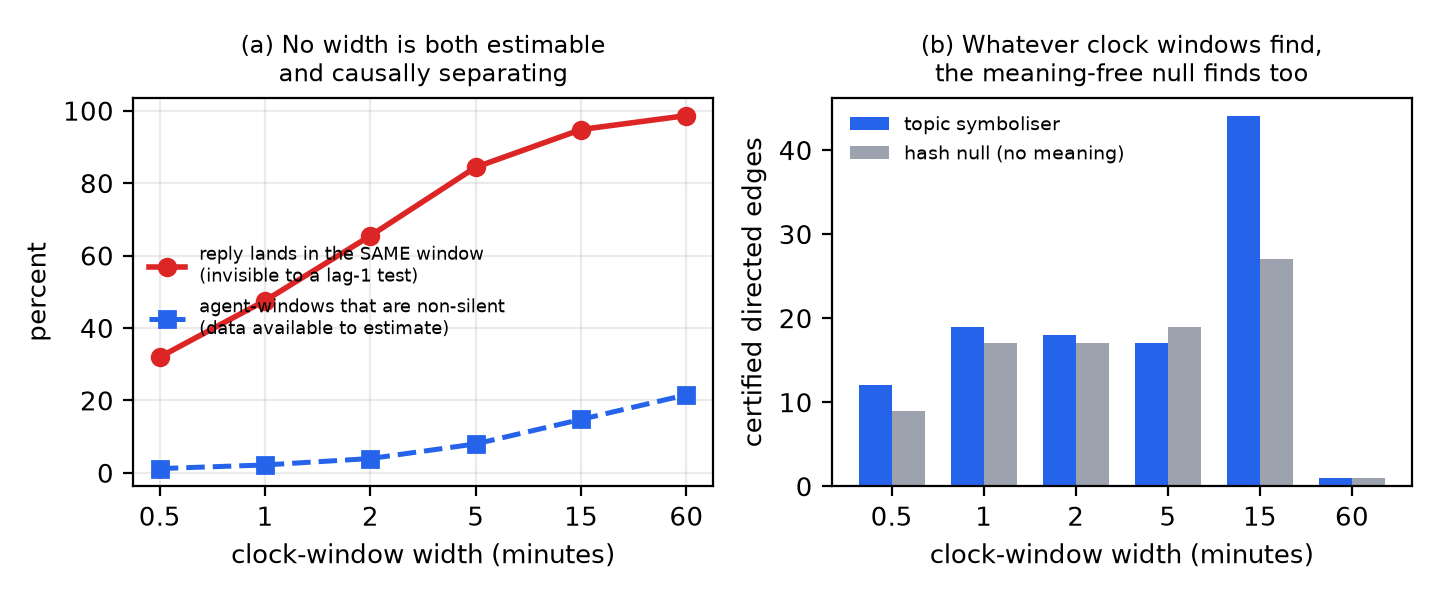
\includegraphics[width=0.92\textwidth]{f1_clock.png}
\caption{Clock-window transfer entropy on the 15 analysed agents of main-village \#general. Left,
the two failure modes as a function of window width. Right, edges certified under the topic
symboliser against the meaning-free hash null.}
\end{figure}

The bind is avoided by ordering messages canonically and letting one message be one tick. Each
agent's series carries its symbol where it spoke and a silent symbol elsewhere, so the lag-1
comparison is between a message and the one immediately before it. The cost is that the measure
captures immediate-predecessor influence only.

\section{The surrogate failure, and two explanations that did not hold}
\label{sec:failure}

An agent is planted into the real stream, drawing its symbols from the channel's marginal and
coupled to nothing at all. It is certified as driving something in 3 of 8 runs when it posts 50
messages, and in 8 of 8 at 100, 263, 600 and 1500 messages, with the mean largest $z$ rising from 5.6
to 12.3, 21.7, 38.3 and 71.7. The error grows with how much the agent speaks, which rules out a
small-sample explanation.

A planted agent could be dismissed as artificial, so the error rate is also measured directly.
Keeping the real speaker sequence and permuting the symbols globally leaves data with no directed
topical influence by construction. The shift surrogate certifies at least one edge in 9 of 10 such
replicates, a family-wise error rate of 0.90 against a nominal 0.05.

\paragraph{What breaks it is the speaker sequence.} Destroying one structure at a time isolates the
cause. Keeping the real speaker order and shuffling only symbols, the shift surrogate fires in 10 of
10 replicates; randomising the speaker order as well drops it to 0 of 10; uniform symbols with the
real order still give 6 of 10. So the driver is the structure of the speaker sequence, not the
symbol distribution and not sparsity. That sequence is far from random in two ways at once: it
repeats a speaker 36\% of the time and returns after one message 38\% of the time, and each agent's
activity is strongly non-stationary, with a median block-share coefficient of variation of 0.79.
Shuffling the order destroys both at once, so this ablation cannot say which of the two mattered.

\subsection{Two explanations I proposed, and the benchmark refuted both}

I initially attributed the failure to mutual exclusivity: only one agent can speak at each tick, so
shifting individual timelines could create overlaps that never occurred in the original
conversation. The benchmark did not support this explanation. A generated channel with exactly one
speaker per tick and steady activity produced an error rate of just 0.025, 95\% Wilson
$[0.011, 0.057]$, far below the 0.90 observed in the real data. Mutual exclusivity alone therefore
cannot explain the failure.

I then suspected turn-taking. In the real channel, speakers repeat 36\% of the time and return after
exactly one message 38\% of the time. However, adding a Markov speaker chain to the generator
produced the opposite result. Turn-taking suppressed the error rather than increasing it. At the
nominal knob values and with no drift the surrogate certified nothing at all across 200 replicates,
while removing turn-taking and introducing drift raised the rate to 0.365. The contribution from
drift was $+0.340$, compared with $-0.025$ for turn-taking. The same inversion appears in the arm
calibrated so that the generated channel reproduces the real channel's measured repeat, return and
block-share statistics rather than merely carrying those numbers as settings: there, turn-taking
alone also certifies nothing, and drift alone gives 0.065.

Neither mechanism, nor their combination in the tested design, reproduced the real-data error rate of
0.90. The largest cell anywhere in the design is 0.365. The real-data ablation removes turn-taking
and non-stationarity together, while the generator separates them. The results point to
non-stationary activity, but the remaining gap means the mechanism behind the full real-data failure
is not yet established.

Every figure above comes from the run at 200 surrogate draws. The first version of this analysis
used 100, which inflates both nulls on the same 2,400 instances: the circular shift fires 53 times
where the 200-draw run does not, against 18 the other way (exact McNemar $p = 3.9 \times 10^{-5}$),
and the permutation surrogate 83 against 20 ($p = 2.7 \times 10^{-10}$). Every qualitative conclusion
in this section is the same at both settings, which is why they are worth stating at all. The
numbers are not, so the draw count belongs in the caption.

\section{The repair, compared}
\label{sec:repair}

Following the local-permutation idea of \citet{runge2018} as adapted by \citet{shorten2021}, each
source keeps its speaking positions and only its symbols are permuted among them. Speaking pattern,
sparsity and turn-taking are preserved exactly, and only the correspondence between symbol and time
is destroyed. On the same destroyed-structure real data the family-wise error rate falls to 0.063
over 300 replicates, 95\% Wilson $[0.041, 0.097]$. The planted uncoupled agent is never certified: 0
of 5 at both 263 and 1500 messages, with mean max $z$ of 2.8 in each case against 22.0 and 68.3
under the shift surrogate.

\begin{figure}[h]
\centering
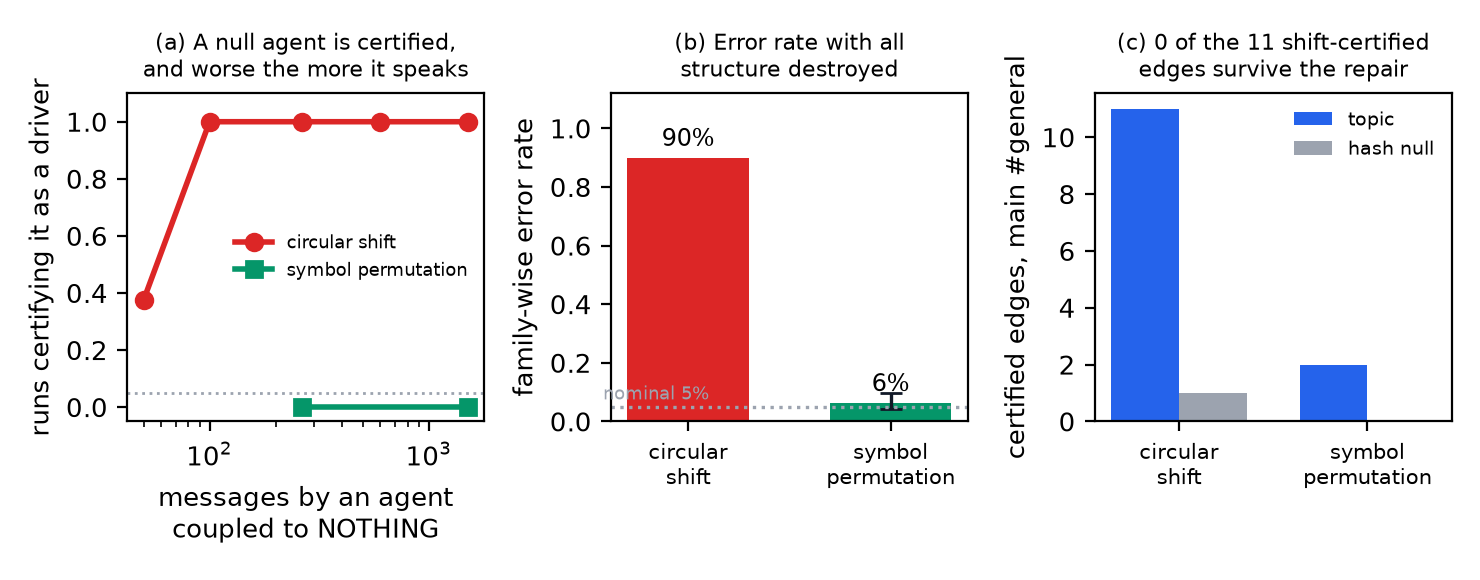
\includegraphics[width=\textwidth]{f2_null.png}
\caption{Left, how often an agent coupled to nothing is certified as a driver, under each surrogate.
Middle, family-wise error rate measured on data with all structure destroyed, with a Wilson
interval; the dotted line is the nominal 0.05. Right, what each surrogate certifies on the real
channel.}
\end{figure}

\subsection{How many surrogate draws are needed}

The number of surrogate draws matters more than I initially appreciated. In a paired comparison of
300 instances, where all four surrogates run on identical symbol grids so the outcomes are paired,
the global permutation surrogate produced a false-positive rate of 0.1167 with 100 draws, falling to
0.0700 with 200 draws, 95\% Wilson $[0.046, 0.105]$. This difference is statistically significant
(exact McNemar $p = 0.0043$). The block-local and Runge local permutations were less sensitive to the
increase: their corresponding rates changed from 0.0900 to 0.0767 and from 0.0967 to 0.0800.

At 200 draws, the global permutation's interval covers the nominal 0.05 and overlaps the real-data
estimate of 0.0633 $[0.0409, 0.0968]$. The real-data result is therefore corroborated rather than
overstated. For practical use, the important point is that reducing the number of surrogate draws
can materially change the result. In particular, the global permutation over-fires at 100 draws by
approximately a factor of two. I would therefore not treat the choice of draw count as a minor
computational detail.

The same correction applies to the benchmark-wide estimate. That figure was 0.0942 at 100 draws.
Repeating all 2,400 instances at 200 draws gives \textbf{0.0679}, 95\% Wilson $[0.0585, 0.0787]$,
and the paired difference is large: 83 instances fire at 100 draws and not at 200, against 20 the
other way, $p = 2.7 \times 10^{-10}$. The conclusion it supports is unchanged, because the interval
still excludes the nominal 0.05. So the permutation repair does carry a residual inflation on clean
generated data, but it is about a third above nominal rather than nearly double.

One limit on this recommendation. I compared 100 draws against 200 and did not test any larger
value, so what the experiment establishes is that 100 is too few, not that 200 is enough. Two
hundred is a lower bound on the draw count rather than a converged setting, and a practitioner whose
conclusions sit near a decision boundary should check their own sensitivity rather than adopt the
number.

\subsection{Choosing a repair, when the error rate cannot choose}

The comparison of the three permutation-based repairs does not produce a clear winner. All four
surrogates were evaluated on identical symbol grids across 300 pure-null replicates, so the
comparison reflects differences between the null models rather than differences between datasets.

\begin{table}[h]
\centering
\begin{tabular}{lrrrl}
\toprule
surrogate & FWER, 100 draws & FWER, 200 draws & 95\% Wilson at 200 & nominal 0.05 \\
\midrule
circular shift                   & 0.0433 & \textbf{0.0333} & $[0.018, 0.060]$ & inside \\
global within-speaker permutation & 0.1167 & \textbf{0.0700} & $[0.046, 0.105]$ & inside \\
block-local permutation          & 0.0900 & \textbf{0.0767} & $[0.052, 0.112]$ & excluded \\
local permutation \citep{runge2018} & 0.0967 & \textbf{0.0800} & $[0.054, 0.116]$ & excluded \\
\bottomrule
\end{tabular}
\caption{Four surrogates on identical symbol grids, 300 pure-null replicates, at both draw counts.}
\end{table}

At 200 draws, paired on the same 300 instances, the circular shift is not significantly different
from the global permutation ($p = 0.0614$), although it differs from block-local permutation
($p = 0.0294$) and from Runge's local permutation ($p = 0.0201$). At 100 draws it differed from all
three, which is the draw-count artifact again. The three repairs remain statistically
indistinguishable from one another, with pairwise $p$-values of 0.85, 0.65 and 1.00. The apparent
differences in their error rates are not sufficient to establish a ranking.

Choosing between them therefore requires more than calibration, and two readings pull against each
other. Runge's local permutation has the strongest methodological justification for preserving the
structure it is intended to preserve, and it follows the approach adapted to event data by
\citet{shorten2021}. Block-local permutation is more heuristic and introduces a free parameter that
has not been tuned. Global permutation is the simplest. On the other hand, the global permutation has
the most favourable interval relative to the nominal rate, and is the only repair that costs nothing
measurable against the shift on clean stationary data, although neither difference is statistically
established. I do not consider the observed error rates sufficient to select one repair over the
others. The choice should be guided by the structure the null is intended to preserve and the
assumptions that can be justified for the data.

\subsection{When to use the repair}

A drift sweep gives the practical reading. Across 150 replicates per cell at 200 surrogate draws,
the circular shift degrades steadily as activity drift increases while the three repairs do not.

\begin{table}[h]
\centering
\begin{tabular}{lrrrr}
\toprule
activity drift & circular shift & global permutation & block-local & local \\
\midrule
0.0 & \textbf{0.013} & 0.093 & 0.080 & 0.093 \\
0.3 & 0.100 & 0.100 & 0.093 & 0.120 \\
0.6 & \textbf{0.193} & 0.053 & 0.047 & 0.067 \\
0.9 & \textbf{0.380} & 0.087 & 0.080 & 0.080 \\
\bottomrule
\end{tabular}
\caption{Family-wise error on pure nulls as activity drift increases, 150 replicates per cell, 200
surrogate draws. Every certified edge is a false positive by construction.}
\end{table}

The pattern is supported by a formal trend test rather than by eye. A Cochran-Armitage test across
the four ordered drift levels gives the circular shift $z = 8.667$, $p < 10^{-15}$, and gives every
repair nothing: $p = 0.51$ for the global permutation, 0.63 for block-local and 0.37 for local. The
same pattern holds at both surrogate draw counts, so it does not depend on that choice.

The repairs are therefore flat under drift rather than calibrated. Only one of the four global
permutation intervals covers the nominal 0.05, and the rest sit nearer 0.09, so what the repair buys
is insensitivity to drift rather than correctness. One asymmetry should be stated rather than
hidden: block-local covers nominal in three of the four cells where the global repair covers one.
The two remain pairwise indistinguishable, so this is not grounds to switch the recommendation, but
it does mean the global repair cannot be described as the best-calibrated under drift.

The results also show why the repair should not be treated as universally preferable. At zero drift
the circular shift has an error rate of 0.013, while the three repairs are all around 0.08 to 0.09.
That advantage is gone by the first drift step: at drift 0.3 the shift reads 0.100 against the global
permutation's 0.100 and block-local's 0.093, so the crossover falls between drift 0.0 and 0.3 rather
than at some higher level. By drift 0.6 the shift is roughly four times the repairs. If a channel has
been checked and found stationary, the circular shift may be sufficient. When activity is
non-stationary the repairs are the more stable choice, and the margin for error on that judgement is
narrow, because the crossover arrives by the first drift level tested.

\section{Continuous time, and what the repair cannot test}

An earlier analysis identified continuous-time estimation as the principled option for event data
but did not evaluate it. Running the continuous-time estimator CoTETE on both channels certifies 0
edges in either case, compared with 2 for main-village and 18 for open-chat under the discrete,
turn-ordered analysis. Its highest $z$-scores are 3.062 and 3.980, below the respective max-T
thresholds of 4.171 and 4.308.

At first these results might appear to contradict the symbol-based analysis. The two estimators
operate on different information, however. CoTETE's public API takes event times with no symbol
channel, while the transfer-entropy analysis here uses topic symbols. To test whether this
difference explains the results, I reduced the data to timing alone, replacing every spoken symbol
with the same code. Under this representation the estimator used here also detects 0 edges in both
channels, matching CoTETE. Using the circular-shift surrogate instead produces 12 and 3 edges. So
neither method detects relationships from event timing alone in these channels, and the edges found
by the symbol-based analysis depend on symbol correspondence, which the continuous-time estimator
cannot access.

Two caveats attach to those $z$-scores, and the second attaches to the larger of them. Point
estimates from this estimator are stochastic to about 17\% across repeated runs, so none of these
values should be read to more than two significant figures. And open-chat's highest $z$, the 3.980,
belongs to the one pair whose surrogate draws mostly failed: it needed 1,936 failed draws to obtain
100 successes, a 4.9\% success rate. Those surrogates are conditioned on being estimable, so that
pair's null is biased in an unknown direction. The conclusion does not rest on it, since that pair
falls below threshold and so does every other pair, but the number should not be quoted as a clean
measurement. The failures themselves were a defect rather than a property of the data: an enlarged
exclusion window can empty the neighbour search on sparse bursty event trains and raise an error
that terminates a whole pair, with no handling at the public entry point. This has been reported
upstream.

There is also a fundamental limitation in applying the recommended permutation surrogate to
timing-only data. When every event carries the same symbol, permuting those symbols changes nothing.
The observed statistic and the surrogate null are identical, making the test exactly degenerate:
standard deviation 0 across all 210 pairs and $p = 1.0$ everywhere. \textbf{The repair has zero power
against timing structure by construction.} The permutation surrogate is appropriate for testing
relationships in the symbol sequence, but it does not answer whether relationships exist in event
timing. These are different questions, and choosing one null means giving up the ability to test the
other with that procedure.

\section{Confounding, and what conditioning removes}

A valid surrogate fixes calibration but not confounding. If every agent tracks a drifting channel
topic, every pair is genuinely dependent through the channel, and pairwise transfer entropy cannot
tell that from direct influence. I therefore also report a \textbf{conditional} estimate, which asks
whether a source's last message adds anything about a target's next one beyond the target's own
history and the channel's recent state. The conditioning variable is the modal symbol of the last
twelve messages, excluding the immediately preceding one so that it does not simply restate the
source.

On a generated benchmark whose decisive instances contain no influence while every agent tracks a
shared drifting topic, so that any certified edge is common cause, pairwise transfer entropy
certifies \textbf{22.3} edges on average and conditioning takes that to \textbf{0.33}, lifting pooled
precision on the four-edge instances from 0.17 to \textbf{0.80} at a recall of 1.0 either way. Across
couplings from 0.05 to 0.8 the conditional test still finds the planted edge in 3 of 3 runs, so the
gain costs no power.

The benchmark flatters the conditional estimator, since its common cause is a shared modal topic and
the conditioning variable is the channel's modal topic. The real channels are harder, and
conditioning there costs degrees of freedom: a 9-symbol alphabet with a 9-valued context gives 6,561
cells against about 7,900 ticks, so that variable is also coarsened to 4 and 2 values.

\begin{table}[h]
\centering
\begin{tabular}{lrrrr}
\toprule
channel & pairwise & conditional, 9 values & 4 values & 2 values \\
\midrule
main \#general      & 2  & \textbf{2, the same two edges} & 2 & 3 \\
open-chat \#general & 18 & \textbf{0} & \textbf{7} & \textbf{13} \\
swarm, room a       & 1  & \textbf{0} & & \\
\bottomrule
\end{tabular}
\caption{Conditioning at three resolutions. Main-village's two edges are robust to that choice;
open-chat's zero is not.}
\end{table}

At the finest resolution the open-chat test is degenerate, its surrogate sitting above the observed
statistic for 65\% of pairs with the largest $z$ in the family only 4.4, so it is failing to reject
rather than finding nothing to reject. Open-chat's structure therefore remains
\textbf{undetermined}: depending on the conditioning resolution, between 0 and 13 of its 18 edges may
survive. That resolution is a free parameter an analyst would set once and never revisit. This is a
property of the channel rather than the estimator: on structure-free real data the conditional test
fires in 2 of 40 replicates, an error rate of 0.05 with a mean $z$ of $-0.001$, so it is nominal
rather than conservative.

\section{The symbolisation floor}
\label{sec:floor}

Everything these methods produce is downstream of turning text into symbols. On the benchmark, where
the underlying topics are known, detection performance drops sharply when agreement between the
symboliser and the ground truth falls below roughly ARI 0.44, and this behaviour appears across the
tested estimators. Importantly, the false-positive rate can look \emph{better} below this point,
because the shared topic structure needed to produce confounded detections is no longer represented
reliably. A pipeline that stops detecting relationships may therefore have lost the signal it needs
rather than become more reliable, and nothing downstream of the symboliser can tell those apart.

\subsection{Detecting the floor without labels}

That degradation can be detected without ground-truth labels. Across the nine-level benchmark sweep,
three statistics separate the below-floor cases with zero errors: seed stability at a threshold of
0.623, agreement with LSA at 0.646, and the Calinski-Harabasz index at 138.9. Seed stability here is
the \textbf{minimum} pairwise agreement across seeds, not the mean; the mean variant makes one error,
at a different threshold of 0.791. Silhouette has the strongest correlation with true ARI, at 0.979,
but is not useful for identifying the boundary because its threshold falls within a gap of just
0.002. A statistic that tracks clustering quality most closely is not necessarily the best one for
making a classification decision.

Error count cannot choose among the three that were perfect, so I tested whether each threshold still
means what it meant when the channel changes for reasons other than topic separability. Applying each
cut unchanged to thirty cells that vary turn-taking, drift, agent count, volume skew, message length
and corpus size, twenty-seven of which hold true ARI at exactly 1.000:

\begin{table}[h]
\centering
\begin{tabular}{lrrrr}
\toprule
diagnostic & cut & errors where fitted & errors, nuisance set & of those at true ARI 1.000 \\
\midrule
seed stability, min across seeds & 0.623 & 0 & 2 & \textbf{0} \\
LSA agreement                    & 0.646 & 0 & 2 & \textbf{0} \\
Calinski-Harabasz                & 138.9 & 0 & 6 & \textbf{3} \\
\bottomrule
\end{tabular}
\caption{Whether a cut fitted on the vocabulary-overlap mechanism survives a change in the channel
that is not a change in topic separability.}
\end{table}

The two bounded statistics err only on the short-message cells, where the symbolisation genuinely has
degraded. Calinski-Harabasz additionally condemns all three cells whose true ARI is exactly 1.000,
for no reason beyond the corpus holding 2,000 messages rather than 8,000, where it reads 76 to 77
against its own cut of 138.9. It is unbounded and grows with sample size, so a published numeric
threshold for it carries no meaning on another corpus. That is why I recommend the two bounded
statistics and not the index that matched them on error count. \textbf{A cut that moves with the
corpus is not a floor cut.}

This is not a weak statistic being discarded on a technicality. Calinski-Harabasz correlates with
true ARI at 0.973, almost as closely as silhouette, and unlike silhouette it classifies the floor
perfectly where it was fitted. It still cannot carry a published threshold. That is the sharper form
of the point above: neither the statistic that tracks quality most closely nor the one that
classifies best on the fitting mechanism is necessarily the one whose cut another researcher can
reuse.

There are important limits to this result. The effective sample size is nine rather than 54, because
the classification label is determined by overlap level. There are no observations between ARI 0.444
and 0.222, so the exact location of the boundary within that interval remains unknown. These
diagnostics classify whether a result is below the tested detection floor; they do not estimate ARI,
and their behaviour is flat between 0.68 and 1.00, and not even monotone there. The benchmark also
uses a single degradation mechanism with a known and correct value of $k$, whereas the true number of
topics in real conversations is unknown. I therefore treat 0.44 as a benchmark-specific, bracketed
result rather than a universal threshold.

\subsection{A contradiction the diagnostic lost}

I initially used these diagnostics to classify one real channel, open-chat, as below the
symbolisation floor. That conclusion did not agree with the channel's measured results: open-chat
certified 18 and 22 edges under the two symbolisers, compared with 2 and 1 for main-village, and its
hash-based null certified zero edges. Rather than treating this disagreement as evidence that the
original measurements were wrong, I revisited the diagnostic itself.

The problem was the choice of $k$. Repeating the comparison with the same channels, loader and window
reproduced the published $k=8$ results to the digit. At $k=4$, however, open-chat reached stability
scores of 0.950 and 0.978, the highest values produced by either channel across the tested settings,
and both exceeded the diagnostic thresholds. The earlier below-floor classification was therefore a
conclusion about one arbitrary choice of $k$, not a reliable statement about the channel. Message
length does not explain the difference either: 27.1\% of main-village messages contain fewer than
five tokens, compared with 2.3\% in open-chat, so the short-message channel is the one the diagnostic
cleared.

This correction changes how the symbolisation results should be read, and it withdrew three claims.

\begin{enumerate}
\item \textbf{The claim that no topic signal remains below the floor is too strong.} The
circular-shift surrogate recovers all four planted edges at every tested overlap level, including
0.95, where ARI is 0.011. The observed collapse is in the permutation null, not necessarily in the
underlying data.
\item \textbf{ARI 0.44 cannot be treated as a universal detection threshold.} When the shared-topic
parameter is 0, detection continues down to ARI 0.296, so the boundary depends on both the
symboliser and the channel.
\item \textbf{Edge counts cannot be used as a measure of symboliser quality.} Even at ARI exactly
1.000, changing the shared-topic parameter alone moves the permutation edge count from 5 to 78.
\end{enumerate}

The diagnostics also do not transfer reliably outside the mechanism on which they were evaluated.
Their balanced accuracy falls from 1.00 to 0.75 and 0.571 under a known mismatch in $k$. All seven
errors made by seed stability are false below-floor classifications, and in every one of those cases
the detector still identifies all planted edges; of the fourteen cells it condemned, eleven had full
conditional recall. The failure direction is the dangerous one: it condemns working symbolisations.

This was an important correction to my own interpretation. I introduced a diagnostic to check whether
the symbolisation was reliable, applied it to the real channels, and found that it contradicted
measurements already in hand. Investigating that contradiction showed the diagnostic was sensitive to
an arbitrary modelling choice. The result is not that the original measurements were wrong, but that
the control was being asked to support a broader conclusion than the evidence allowed. These
diagnostics remain useful within their tested setting, and \textbf{no channel-level floor verdict
should be issued from a single $k$}.

\section{The benchmark}

Real logs have no ground truth, so the common-cause question could not be settled on them. The
generator used here makes the influence graph known by construction: it decides, in code, who speaks
at which tick, on which topic, and who reacts to whom. Surface text is a separate, replaceable layer
drawn from disjoint per-topic vocabularies, so the whole thing runs offline and a detector still has
to symbolise raw text rather than read the labels. Turn-taking and activity drift are independent
knobs, so the two can be varied one at a time, and the generator reproduces its earlier behaviour
bit for bit when both are zero.

\benchname{} is released with 150 tests covering the generator, the detector harness, the text layer,
the floor analysis and the turn-taking factorial.
\ifdeanon{Code and benchmark:
\url{https://github.com/manunicholasjacob/swarm-influence-bench} and
\url{https://github.com/manunicholasjacob/swarm-influence-audit}.}{Code and benchmark are publicly
released; the links are withheld here for anonymity and will be given in the camera-ready version.}

One property of the benchmark must be stated when its numbers are quoted. Planting an edge displaces
other agents' speaking turns, so the generated instances contain real lag-1 dependencies that the
label set does not list. Precision measured against those labels is therefore a \textbf{lower bound}
for any detector, and what the benchmark supports is the comparison between two estimators rather
than the absolute value of either.

\section{What an overseer should do}

Six inexpensive controls should be included whenever an influence graph over an agent channel is
published.

\begin{enumerate}
\item \textbf{Plant an agent coupled to nothing, at your channel's volumes, and check it is not
certified.} This one test would have caught the failure reported here, at one run per volume.
\item \textbf{Measure the error rate directly}, by destroying the structure your method claims to
find and checking the family-wise rate is near nominal. If it is not, your surrogate does not match
your data.
\item \textbf{Preserve the speaker sequence in your surrogate.} Any surrogate that moves an agent's
messages in time will disturb it, and \citet{shorten2021} is the principled route. Use at least 200
surrogate draws, because at 100 the global within-speaker permutation over-fires by roughly a factor
of two.
\item \textbf{Establish the detection floor before interpreting an absence.} ``No edges'' and ``no
influence'' are different claims.
\item \textbf{Condition on the channel, report both numbers, and sweep the resolution.} Pairwise and
conditional bound the answer, and the gap between them is the result. Conditioning costs cells, so
check whether your answer is an artifact of how finely you conditioned. On one channel here it was.
\item \textbf{Report how well your symboliser agrees with the truth, on data where you know it.}
Everything is downstream of turning text into symbols, and below roughly ARI 0.44 detection
collapses whatever the estimator. I have found this control in no influence-detection paper, and it
is also the one that cannot be run on real logs, which is why the floor remains the largest
unquantified threat here.
\end{enumerate}

Two habits follow: publish a meaning-free null's count beside the real one, and require held-out
replication before calling a graph a structure.

\section{The real channels, and what survives}

Re-running every channel under the repaired surrogate changes the answers, and not in one direction.

\begin{table}[h]
\centering
\begin{tabular}{lrrr}
\toprule
channel & window messages & shift: topic / hash & permutation: topic / hash \\
\midrule
main \#general      & 8,800 & 11 / 1 & 2 / 0 \\
open-chat \#general & 8,226 & 3 / 0  & 18 / 0 \\
swarm, room a       & 3,846 & 2 / 1  & 1 / 0 \\
\bottomrule
\end{tabular}
\caption{The same channels under both surrogates, with the meaning-free hash null beside each.}
\end{table}

In main-village, \textbf{none} of the 11 edges the standard recipe certifies survives the repair, and
the two the valid surrogate certifies were not among them. In open-chat the correction runs the other
way, 3 edges becoming 18, because pathological pairs inflate the max-T threshold and raise the bar
for everything else. An invalid surrogate does not simply add false positives; it scrambles the
result.

Main-village's two edges are the strongest thing here and they are still not a finding, because they
do not replicate: the adjacent fourteen-day window certifies nothing at all under either estimator.
Given the detection floor, that silence is as consistent with the test sitting near its limit as with
the edges being absent, and the two cannot be separated. Power is governed by how much an agent says
as much as by how strongly it copies, and it is channel-specific: in main-village a planted follower
copying on 80\% of its messages is caught only 1 time in 4, while in open-chat one copying 10\% of
the time is caught 3 times in 4. Replication is weak everywhere: under the standard recipe the
adjacent window shares 1 edge out of 8 and 4, and that edge is also the only one the hash null
certifies. No certified edge in this work replicates out of sample.

\begin{figure}[h]
\centering
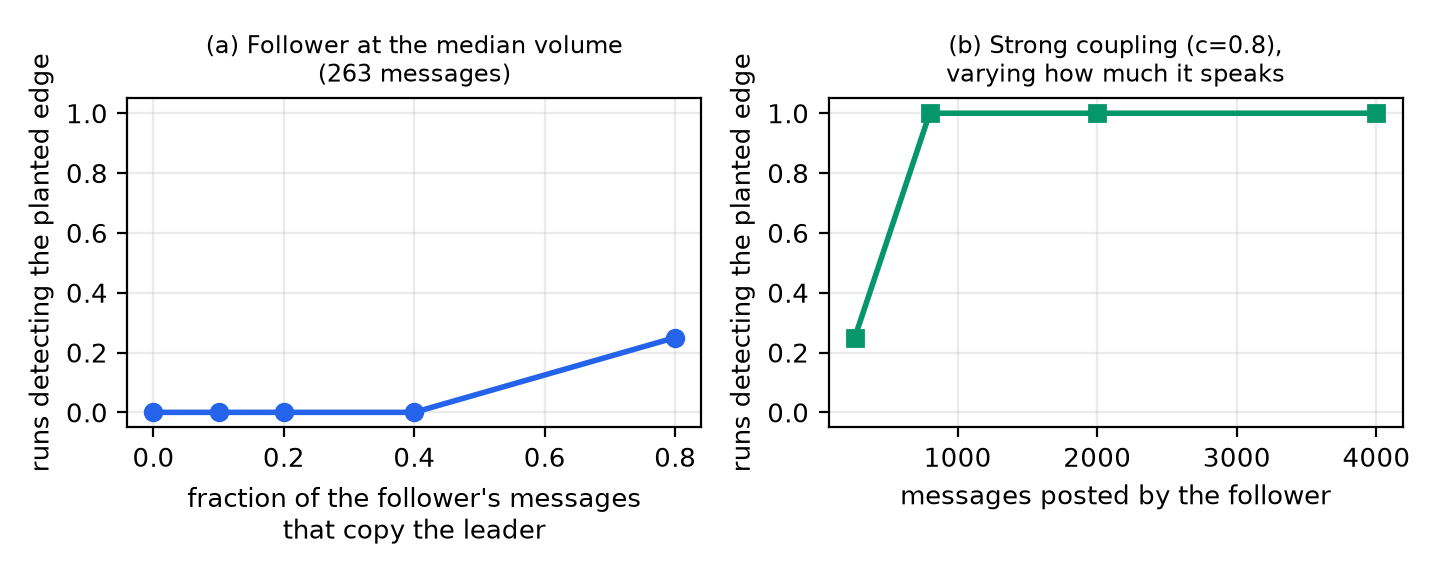
\includegraphics[width=0.92\textwidth]{f4_power.png}
\caption{Detection of a planted follower under the repaired surrogate. Left, varying the fraction of
its messages that copy the leader, at the median agent's volume. Right, varying how much it speaks,
at strong coupling.}
\end{figure}

\paragraph{Humans in the channel.} Main-village \#general is now effectively human-free, with 3 human
messages in the window, so the question has to be asked in open-chat, where 32\% of messages come
from 124 human visitors. Pairwise, with humans collapsed into one node, 19 edges are certified.
Conditioning removes almost all the agent-to-agent structure and little of the rest: \textbf{four
edges survive, of which three run from humans to agents, one is agent to agent, and none run from an
agent to a human.} The asymmetry is not an artifact of the confound. It should be read carefully all
the same: topical dependence from a person to an agent is also what ordinary responsiveness looks
like, so the measurement supports only that the dependence is dyad-specific and directional, not
that anyone is steering a swarm.

\section{Reproducibility, and one limitation of it}

Every number in this paper is recomputed from committed analysis output by a verifier that fails on a
mismatch, and that verifier covers the prose of this paper as well as the figures.

One limitation should be stated plainly. Re-running the counts in the earlier stationarity sweep with
the same seeds and configuration, only one of the eight cells reproduced exactly; the remaining
differences were one or two replicates per cell. Seven of the eight published rates still fell within
the recomputed Wilson intervals, and no conclusion changed. The exception is the zero-drift cell under
the permutation null, where the published 1 of 30 falls just below the recomputed interval of
$[0.035, 0.256]$ for 3 of 30, and no result here depends on that cell.

The generator, estimator and BLAS configuration were investigated and ruled out as the source. The
most likely explanation is a library-level difference, particularly in scikit-learn's $k$-means
implementation within the symboliser, whose output can vary between versions. Every sweep now records
the environment it ran under: Python 3.14.6, numpy 2.5.1, scipy 1.18.0 and scikit-learn 1.9.0,
including the BLAS build and the number of BLAS threads each worker used.

This does not make the previously published counts exactly reproducible. It provides a more clearly
specified environment in which subsequent results can be checked. For that reason I report rates
alongside their confidence intervals rather than exact replicate counts. The distinction between
reproducing a result within its uncertainty and reproducing every individual count matters, and only
the first is claimed.

\section{Conclusion}

Applied to real agent chat, the standard recipe for ``who drives whom'' needs repair before it says
anything. Clock windows cannot separate a message from its answer at the speed agents reply, and what
they certify is matched by a null with no access to meaning. The turn-ordered grid that fixes this
breaks the circular-shift surrogate: family-wise error 0.90 against a nominal 0.05, caused by the
speaker sequence itself. Restricted permutation surrogates repair most of that, but they are flat
under drift rather than calibrated, they are mutually indistinguishable at this precision, and one of
them needs twice the surrogate draws anyone would think to use. A valid surrogate fixes calibration
but not confounding. What survives is small: two dyad-specific edges that do not replicate, an
undetermined answer set by conditioning resolution, and influence running from people into agents and
never back. \textbf{An influence graph should not guide decisions until its error rate, its confound,
its detection floor and its symboliser's fidelity are reported.}

\section*{Limitations}

\begin{itemize}
\item \textbf{Immediate-predecessor only.} The turn-ordered lag-1 measure sees influence from the
message directly before a reply. Influence acting over several turns, or through a room's accumulated
context, is out of scope.
\item \textbf{Discrete approximation to an event process.} Agent chat is event-based in continuous
time. The turn-ordered discretisation with a permutation surrogate is a practical fix, and the
continuous-time comparison above shows what that choice gives up.
\item \textbf{The mechanism behind the real 0.90 is not established.} The generator separates
turn-taking from drift and points at drift, but the largest cell anywhere in the design is 0.365.
\item \textbf{Symbolisation quality cannot be measured on the real logs.} The central result survives
an independent symboliser, but the edge count does not: it moves with alphabet size and with which
messages the topic model is fit on. The floor remains the largest unquantified threat.
\item \textbf{No ground truth in the real logs.} The validity argument rests on planted controls and
on the meaning-free null, not on recovering a known answer.
\item \textbf{Conditioning removes real influence too.} The conditional estimate discards influence
that works by shifting what the channel is talking about, which in a group chat may be a large part
of genuine influence. It is a lower bound on dyadic influence.
\item \textbf{The human result is exploratory.} It rests on one village and one window and should be
read as a lead.
\end{itemize}

\section*{Broader impact and ethics}

This work audits influence detection on a population of AI agents, which is dual-use. Used
defensively it helps an overseer decide what an influence graph is worth, and the main result is
deflationary: it tells practitioners to trust these outputs less, which reduces rather than increases
the chance of acting on a bad attribution. The same tooling could be used to identify the most
influential agent in a swarm in order to target it, or to surveil participants in a channel. Three
properties limit the misuse. The subjects are AI models; the dataset is already public under research
terms and no re-identification is added; and the measure is weak and local, recovering
immediate-predecessor topical dependence rather than any model of how to steer an agent.

The dataset's research terms were followed: research use only, no training on the data, no
re-identification, citation of the source, and notification of the authors of resulting publications.
Human participants appear only as an aggregate node or as anonymised visitor labels, never by name or
handle, and no content attributable to an individual person is reported. Message text and metadata
were read, never model weights or private user data.

The use of a large language model in this work is disclosed in the first-page footnote, as TMLR
requires.

\bibliographystyle{tmlr}
\bibliography{refs}

\end{document}
"               de-anonymised arXiv preprint
%   pdflatex "\def\TMLRMODE{accepted}% TMLR submission. Built 10 November 2026 from:
%   paper/00_PROSE_v1.md   the author's written sections, 78 figures auto-verified
%   report/REPORT_V2.md    the sprint report, every number recomputed by report/verify_v2.py
%
% ANONYMITY. \usepackage{tmlr} with no option is the anonymous submission mode: the tmlr
% package hides the author block itself. Switching to [preprint] de-anonymises for arXiv AND
% turns on the \ifpreprint branches below, which are the only places a name, a repository URL
% or the benchmark's distinctive name appears. So one source produces both documents and the
% anonymous build cannot leak an identifier that the preprint build adds.
%
% Build:  latexmk -pdf main.tex
\documentclass[10pt]{article}

% The mode is chosen at build time so that one source produces every variant and they cannot
% drift apart:
%   latexmk -pdf main.tex                                        anonymous TMLR submission
%   pdflatex "\def\TMLRMODE{preprint}\input{main}"               de-anonymised arXiv preprint
%   pdflatex "\def\TMLRMODE{accepted}\input{main}"               camera-ready
% Use build.py, which runs all of them and checks the anonymous output for leaks.
\providecommand{\TMLRMODE}{submission}
\makeatletter
\def\@tmlrpreprint{preprint}
\def\@tmlraccepted{accepted}
\ifx\TMLRMODE\@tmlrpreprint
  \usepackage[preprint]{tmlr}
\else
  \ifx\TMLRMODE\@tmlraccepted
    \usepackage[accepted]{tmlr}
  \else
    \usepackage{tmlr}
  \fi
\fi
\makeatother

\usepackage{hyperref}
\usepackage{url}
\usepackage{booktabs}
\usepackage{graphicx}
\usepackage{amsmath}

% Gate every identifying string on whether identity may be revealed at all. The flag to test is
% \if@accepted, NOT \if@preprint: tmlr.sty's [preprint] option sets BOTH, so \if@accepted is true
% for the preprint and the camera-ready and false only for the anonymous submission, which is
% exactly the condition wanted. Gating on \if@preprint alone also hid the repository URLs from the
% camera-ready, which is where this paper promises to give them. \if@accepted is internal to
% tmlr.sty, hence the \makeatletter. The anonymous build takes the second argument.
\makeatletter
\newcommand{\ifdeanon}[2]{\if@accepted#1\else#2\fi}
\makeatother
\newcommand{\benchname}{\ifdeanon{SwarmInfluence-Bench}{the benchmark}}

% An unmarked footnote, for the LLM-use disclosure. TMLR's FAQ requires the disclosure and names
% the location: authors must "mention explicitly in their submission that they have used this
% tool", "as a footnote on the first page". Verified against jmlr.org/tmlr/faq.html on 10 Nov 2026.
% It is therefore not optional, and it does not belong in Broader Impact, where it sat until now.
% Nothing in the policy asks for the vendor's name, so none is given.
\newcommand{\disclosurefootnote}[1]{%
  \begingroup\renewcommand\thefootnote{}\footnote{#1}\addtocounter{footnote}{-1}\endgroup}

\title{An Influence Graph Over AI Agents Certifies an Agent That Copies Nobody}

% Hidden by the tmlr package unless [accepted] or [preprint] is given.
\author{\name Manu Nicholas Jacob \email manunicholasjacob@gmail.com \\
        \addr Independent Researcher}

\def\month{11}
\def\year{2026}
\def\openreview{\url{https://openreview.net/forum?id=XXXXXXXXXX}}

\begin{document}
\maketitle

\begin{abstract}
Circular-shift surrogates can produce severely inflated false-positive rates when applied to
turn-ordered multi-agent conversations, reaching a family-wise error rate of 0.90 against a nominal
0.05. A generated benchmark separates two candidate mechanisms and points at non-stationary speaker
activity rather than turn-taking, which suppresses the failure rather than causing it. No setting of
either knob reproduces the observed 0.90, however, so what drives the full real-data failure remains
open. Restricted permutation surrogates substantially reduce the problem. Their error rate is flat
with respect to drift rather than at the nominal level, and for the global within-speaker variant it
depends on how many surrogate draws the null is built from. Calibration alone does not address
confounding, which motivates a conditional estimator validated against a benchmark with planted
ground truth. I also identify a symbolisation-dependent detection limit and develop label-free
diagnostics for it, and show that their calibration does not transport across degradation
mechanisms. The benchmark is released.
\end{abstract}

\disclosurefootnote{\textbf{Use of a large language model.} A large language model was used as an
assistive tool: to help write and run the analysis code, and to help draft this paper. The author is
responsible for every claim, number and figure. All results come from the released code run on the
public dataset, no result or reference is fabricated, and every number in this paper is recomputed
from committed analysis output by a verifier that fails the build on a mismatch.}

\section{Introduction}

When AI agents interact in a shared channel, it is useful to understand how they influence one
another. Information-theoretic methods offer a way to measure this through lagged transfer entropy,
surrogate testing, and per-agent influence scores. They are attractive because they require no
labels and no access to model internals, only a record of who said what and when. The reliability of
those measurements is what this paper examines.

Almost every demonstration of these detectors runs on synthetic traces with a planted leader, where
the analyst controls timing and vocabulary. Real agent chat is asynchronous, bursty, and written in
open language. The narrower question here is whether the standard recipe, applied to real agent
logs, returns anything an overseer should act on.

The audit runs on the AI Village corpus \citep{aidigest2026}, in which frontier models share chat
channels over eighteen months across four villages differing in size, lifetime and tempo, applying
the checks a reader should demand: planted controls, a meaning-free symboliser, replication in a
held-out window, and sensitivity to every parameter that had to be chosen.

\begin{enumerate}
\item The conventional circular-shift surrogate is \textbf{invalid} on turn-ordered agent chat: a
family-wise error rate of 0.90 against a nominal 0.05, caused by the structure of the speaker
sequence itself.
\item Restricted permutation surrogates restore most of the calibration, and re-certifying under one
\textbf{scrambles rather than shrinks} the answer: one channel loses all 11 of its edges, another
gains 15.
\item The three restricted variants are \textbf{mutually indistinguishable} at the precision reached
here, so the choice between them cannot be justified on error rate. The global within-speaker
variant additionally needs on the order of 200 surrogate draws, and over-fires by roughly a factor
of two at 100.
\item Calibration is not confounding, so a conditional estimate is added and validated on a released
benchmark with a known influence graph: common-cause false edges fall from 22.3 to 0.33, and on the
planted-edge instances precision rises from 0.17 to 0.80 with no loss of recall or power.
\item The same benchmark exposes a \textbf{symbolisation floor}. Below roughly 0.44 adjusted Rand
index between symboliser and truth, detection collapses whatever the estimator. Label-free
diagnostics detect that floor, but their calibration does not transport across degradation
mechanisms, and I report where it fails.
\item On the real channels two edges stand at every conditioning resolution, 18 are
\textbf{undetermined} between 0 and 13, none replicates out of sample, and what survives alongside
humans runs from people to agents.
\end{enumerate}

\section{Related work}

\paragraph{Transfer entropy and surrogates.} Transfer entropy \citep{schreiber2000} measures how much
a source's past reduces uncertainty about a target's next symbol beyond the target's own past.
Plug-in estimators are biased upward on short series, so significance rests on surrogate data, with
family-wise error controlled by a max-T test \citep{westfall1993}. The usual surrogate is a circular
time shift of the source.

\paragraph{Event-based data breaks the shift surrogate.} \citet{shorten2021}, on neural spike trains,
show that the conventional source-time-shift surrogate fails to represent the null hypothesis of
conditional independence for event-based processes, and adapt to that setting the nearest-neighbour
local permutation scheme of \citet{runge2018}. Agent chat is event-based in that sense: messages are
events in continuous time, not samples of a clocked signal. The correction is not a contribution of
this paper. The contribution is showing that the same failure carries over to multi-agent safety
monitoring, and that it can be severe enough to create apparent leaders where none exist.

\paragraph{The same failure, concurrently, in multi-agent reinforcement learning.}
\citet{papadopoulos2026} report a closely related surrogate failure in multi-agent
reinforcement-learning action series. Their agent pairs have zero influence by construction, yet
circular time shifts produce false-positive rates of 100\% and 98.2\% against a nominal 0.05. A
plain permutation surrogate fares no better in their setting, at 100.00\% and 99.95\%. Their
proposed correction restricts permutations to blocks of training time, which returns the rates to
5.25\% and 5.50\%.

There are important differences between their setting and this one. Their data consist of binary
actions recorded over twelve thousand training rounds, whereas these data are symbolised
natural-language messages arranged on a turn-ordered conversational grid. Their non-stationarity
comes from monotone drift associated with annealing exploration; here the relevant non-stationarity
appears in the speaker sequence. Neither result should be taken as a direct extension of the other.

Nevertheless, the fact that both approaches rely on restricted permutations is worth noting. Their
permutation blocks are defined by training time, while mine are defined by an agent's own speaking
positions. This provides convergent evidence that unrestricted temporal rearrangement can be
problematic in non-stationary multi-agent data. Their findings also serve as a useful warning for
the approach taken here, and the warning has a measured form rather than a rhetorical one: in their
data the unrestricted permutation failed as completely as the time shift, at 100.00\% against a
nominal 0.05. Permutation-based surrogates are not automatically protected against
non-stationarity, and what protects the one used here is the restriction, not the permutation. I
claim no priority over their result and view the two studies as complementary, addressing different
forms of structured multi-agent data.

\paragraph{Oversight under a budget.} AI-control research frames monitoring as resource constrained,
with a cost for false positives \citep{greenblatt2024}. An influence graph is one such measurement,
and its error rate is the concern here.

\paragraph{Clustering stability.} The idea of using clustering stability as a label-free quality
indicator is not new. It has a substantial history, including \citet{benhur2002},
\citet{lange2004}, von Luxburg's review of clustering stability \citep{vonluxburg2010}, and
\citet{tibshirani2005} on prediction strength. What is different in Section~\ref{sec:floor} is the
calibration of these diagnostics against a detection-performance floor rather than against cluster
recovery alone.

\section{Data and representation}

The AI Village dataset ships one gzipped-JSONL table per village. Four villages are used, differing
enough to test whether any finding is a property of one channel.

\begin{table}[h]
\centering
\begin{tabular}{lrrrrl}
\toprule
village & agent messages & agents & lifetime & human messages & busiest room \\
\midrule
main      & 205,726 & 58  & 576 days & 10,029 & \#general (166,715, 81\%) \\
open-chat &  35,483 & 23  &  66 days & 12,264 & \#general (all) \\
swarm     &   3,848 & 133 &   1 day  &      5 & room a (3,846) \\
game-jam  &     838 & 6   &   3 days &     36 & per-team rooms \\
\bottomrule
\end{tabular}
\caption{The four villages. A 2026 scaffolding change scopes each agent to its current room's
context, so the busiest room of each village is a self-contained influence substrate and is analysed
alone.}
\end{table}

The primary window is the final fourteen days of main-village \#general, 17 to 31 October 2026,
holding 8,800 agent messages. Twenty-two models posted at least 50 messages each and the directed
test uses the 15 busiest, giving 7,958 message events. Two scaffolding facts are disclosed rather
than corrected: the automated nudger was off throughout, and the unused \#best and \#rest rooms were
soft-deleted mid-window, which does not touch \#general.

\subsection{From open language to symbols}

Transfer entropy needs discrete symbols, so each message is mapped to a small alphabet before
influence is estimated, and that mapping is kept separate from the estimator. A topic symboliser
(TF-IDF then $k$-means, $k=8$) gives a message its topic cluster id, so paraphrases of one idea share
a symbol. A hash symboliser, a stable hash of the normalised text into $k=8$ buckets, has no notion
of meaning and serves as a null: an edge appearing under both lives in timing alone.

\subsection{The lag problem, and why clock windows cannot solve it}

A lag-1 transfer entropy compares window $t-1$ with window $t$, so influence landing inside one
window is invisible to it. Agent chat makes this binding. Among the fifteen analysed agents the gap
between consecutive messages by different speakers has a median of 28.1 seconds (25th percentile
9.2, 75th 66.2, 95th 159.3), so turn-taking is a seconds-scale process while any clock window wide
enough to hold two speakers is minutes wide and swallows both a message and its answer.

Both horns are measurable. At 30 seconds only 1.2\% of agent-windows hold a message, while 32.0\% of
replies already land in the same window as what they answer, rising to 84.4\% at five minutes. At
every width tried, the meaning-free hash null certifies comparably many edges, and more at five
minutes: 9 against 12 at thirty seconds, 17 against 19 at one minute, 27 against 44 at fifteen, and
19 against 17 at five. Whatever clock-window transfer entropy was detecting there, it was not shared
meaning.

\begin{figure}[h]
\centering
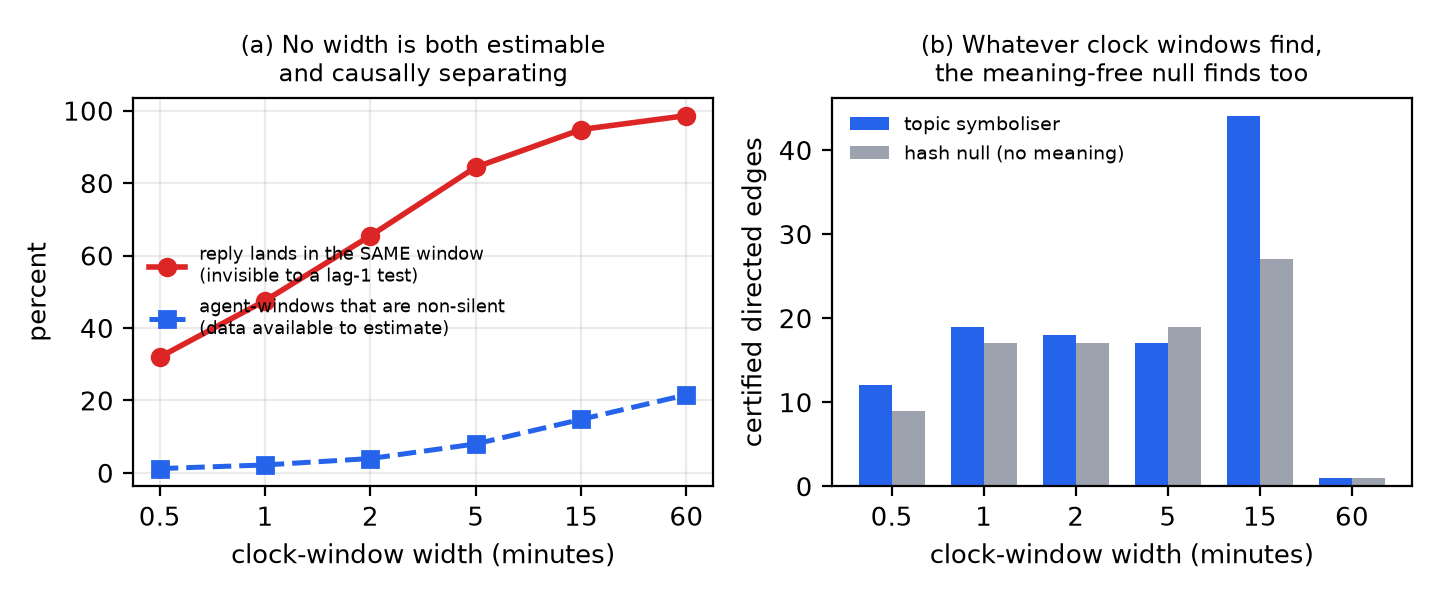
\includegraphics[width=0.92\textwidth]{f1_clock.png}
\caption{Clock-window transfer entropy on the 15 analysed agents of main-village \#general. Left,
the two failure modes as a function of window width. Right, edges certified under the topic
symboliser against the meaning-free hash null.}
\end{figure}

The bind is avoided by ordering messages canonically and letting one message be one tick. Each
agent's series carries its symbol where it spoke and a silent symbol elsewhere, so the lag-1
comparison is between a message and the one immediately before it. The cost is that the measure
captures immediate-predecessor influence only.

\section{The surrogate failure, and two explanations that did not hold}
\label{sec:failure}

An agent is planted into the real stream, drawing its symbols from the channel's marginal and
coupled to nothing at all. It is certified as driving something in 3 of 8 runs when it posts 50
messages, and in 8 of 8 at 100, 263, 600 and 1500 messages, with the mean largest $z$ rising from 5.6
to 12.3, 21.7, 38.3 and 71.7. The error grows with how much the agent speaks, which rules out a
small-sample explanation.

A planted agent could be dismissed as artificial, so the error rate is also measured directly.
Keeping the real speaker sequence and permuting the symbols globally leaves data with no directed
topical influence by construction. The shift surrogate certifies at least one edge in 9 of 10 such
replicates, a family-wise error rate of 0.90 against a nominal 0.05.

\paragraph{What breaks it is the speaker sequence.} Destroying one structure at a time isolates the
cause. Keeping the real speaker order and shuffling only symbols, the shift surrogate fires in 10 of
10 replicates; randomising the speaker order as well drops it to 0 of 10; uniform symbols with the
real order still give 6 of 10. So the driver is the structure of the speaker sequence, not the
symbol distribution and not sparsity. That sequence is far from random in two ways at once: it
repeats a speaker 36\% of the time and returns after one message 38\% of the time, and each agent's
activity is strongly non-stationary, with a median block-share coefficient of variation of 0.79.
Shuffling the order destroys both at once, so this ablation cannot say which of the two mattered.

\subsection{Two explanations I proposed, and the benchmark refuted both}

I initially attributed the failure to mutual exclusivity: only one agent can speak at each tick, so
shifting individual timelines could create overlaps that never occurred in the original
conversation. The benchmark did not support this explanation. A generated channel with exactly one
speaker per tick and steady activity produced an error rate of just 0.025, 95\% Wilson
$[0.011, 0.057]$, far below the 0.90 observed in the real data. Mutual exclusivity alone therefore
cannot explain the failure.

I then suspected turn-taking. In the real channel, speakers repeat 36\% of the time and return after
exactly one message 38\% of the time. However, adding a Markov speaker chain to the generator
produced the opposite result. Turn-taking suppressed the error rather than increasing it. At the
nominal knob values and with no drift the surrogate certified nothing at all across 200 replicates,
while removing turn-taking and introducing drift raised the rate to 0.365. The contribution from
drift was $+0.340$, compared with $-0.025$ for turn-taking. The same inversion appears in the arm
calibrated so that the generated channel reproduces the real channel's measured repeat, return and
block-share statistics rather than merely carrying those numbers as settings: there, turn-taking
alone also certifies nothing, and drift alone gives 0.065.

Neither mechanism, nor their combination in the tested design, reproduced the real-data error rate of
0.90. The largest cell anywhere in the design is 0.365. The real-data ablation removes turn-taking
and non-stationarity together, while the generator separates them. The results point to
non-stationary activity, but the remaining gap means the mechanism behind the full real-data failure
is not yet established.

Every figure above comes from the run at 200 surrogate draws. The first version of this analysis
used 100, which inflates both nulls on the same 2,400 instances: the circular shift fires 53 times
where the 200-draw run does not, against 18 the other way (exact McNemar $p = 3.9 \times 10^{-5}$),
and the permutation surrogate 83 against 20 ($p = 2.7 \times 10^{-10}$). Every qualitative conclusion
in this section is the same at both settings, which is why they are worth stating at all. The
numbers are not, so the draw count belongs in the caption.

\section{The repair, compared}
\label{sec:repair}

Following the local-permutation idea of \citet{runge2018} as adapted by \citet{shorten2021}, each
source keeps its speaking positions and only its symbols are permuted among them. Speaking pattern,
sparsity and turn-taking are preserved exactly, and only the correspondence between symbol and time
is destroyed. On the same destroyed-structure real data the family-wise error rate falls to 0.063
over 300 replicates, 95\% Wilson $[0.041, 0.097]$. The planted uncoupled agent is never certified: 0
of 5 at both 263 and 1500 messages, with mean max $z$ of 2.8 in each case against 22.0 and 68.3
under the shift surrogate.

\begin{figure}[h]
\centering
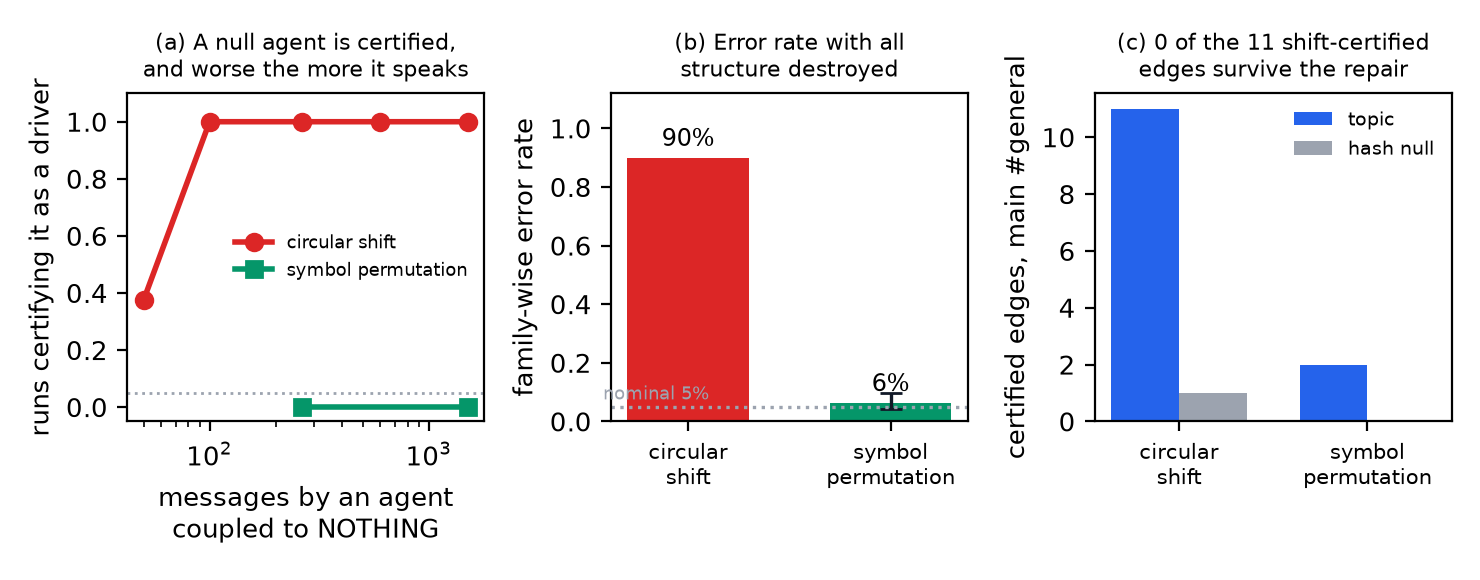
\includegraphics[width=\textwidth]{f2_null.png}
\caption{Left, how often an agent coupled to nothing is certified as a driver, under each surrogate.
Middle, family-wise error rate measured on data with all structure destroyed, with a Wilson
interval; the dotted line is the nominal 0.05. Right, what each surrogate certifies on the real
channel.}
\end{figure}

\subsection{How many surrogate draws are needed}

The number of surrogate draws matters more than I initially appreciated. In a paired comparison of
300 instances, where all four surrogates run on identical symbol grids so the outcomes are paired,
the global permutation surrogate produced a false-positive rate of 0.1167 with 100 draws, falling to
0.0700 with 200 draws, 95\% Wilson $[0.046, 0.105]$. This difference is statistically significant
(exact McNemar $p = 0.0043$). The block-local and Runge local permutations were less sensitive to the
increase: their corresponding rates changed from 0.0900 to 0.0767 and from 0.0967 to 0.0800.

At 200 draws, the global permutation's interval covers the nominal 0.05 and overlaps the real-data
estimate of 0.0633 $[0.0409, 0.0968]$. The real-data result is therefore corroborated rather than
overstated. For practical use, the important point is that reducing the number of surrogate draws
can materially change the result. In particular, the global permutation over-fires at 100 draws by
approximately a factor of two. I would therefore not treat the choice of draw count as a minor
computational detail.

The same correction applies to the benchmark-wide estimate. That figure was 0.0942 at 100 draws.
Repeating all 2,400 instances at 200 draws gives \textbf{0.0679}, 95\% Wilson $[0.0585, 0.0787]$,
and the paired difference is large: 83 instances fire at 100 draws and not at 200, against 20 the
other way, $p = 2.7 \times 10^{-10}$. The conclusion it supports is unchanged, because the interval
still excludes the nominal 0.05. So the permutation repair does carry a residual inflation on clean
generated data, but it is about a third above nominal rather than nearly double.

One limit on this recommendation. I compared 100 draws against 200 and did not test any larger
value, so what the experiment establishes is that 100 is too few, not that 200 is enough. Two
hundred is a lower bound on the draw count rather than a converged setting, and a practitioner whose
conclusions sit near a decision boundary should check their own sensitivity rather than adopt the
number.

\subsection{Choosing a repair, when the error rate cannot choose}

The comparison of the three permutation-based repairs does not produce a clear winner. All four
surrogates were evaluated on identical symbol grids across 300 pure-null replicates, so the
comparison reflects differences between the null models rather than differences between datasets.

\begin{table}[h]
\centering
\begin{tabular}{lrrrl}
\toprule
surrogate & FWER, 100 draws & FWER, 200 draws & 95\% Wilson at 200 & nominal 0.05 \\
\midrule
circular shift                   & 0.0433 & \textbf{0.0333} & $[0.018, 0.060]$ & inside \\
global within-speaker permutation & 0.1167 & \textbf{0.0700} & $[0.046, 0.105]$ & inside \\
block-local permutation          & 0.0900 & \textbf{0.0767} & $[0.052, 0.112]$ & excluded \\
local permutation \citep{runge2018} & 0.0967 & \textbf{0.0800} & $[0.054, 0.116]$ & excluded \\
\bottomrule
\end{tabular}
\caption{Four surrogates on identical symbol grids, 300 pure-null replicates, at both draw counts.}
\end{table}

At 200 draws, paired on the same 300 instances, the circular shift is not significantly different
from the global permutation ($p = 0.0614$), although it differs from block-local permutation
($p = 0.0294$) and from Runge's local permutation ($p = 0.0201$). At 100 draws it differed from all
three, which is the draw-count artifact again. The three repairs remain statistically
indistinguishable from one another, with pairwise $p$-values of 0.85, 0.65 and 1.00. The apparent
differences in their error rates are not sufficient to establish a ranking.

Choosing between them therefore requires more than calibration, and two readings pull against each
other. Runge's local permutation has the strongest methodological justification for preserving the
structure it is intended to preserve, and it follows the approach adapted to event data by
\citet{shorten2021}. Block-local permutation is more heuristic and introduces a free parameter that
has not been tuned. Global permutation is the simplest. On the other hand, the global permutation has
the most favourable interval relative to the nominal rate, and is the only repair that costs nothing
measurable against the shift on clean stationary data, although neither difference is statistically
established. I do not consider the observed error rates sufficient to select one repair over the
others. The choice should be guided by the structure the null is intended to preserve and the
assumptions that can be justified for the data.

\subsection{When to use the repair}

A drift sweep gives the practical reading. Across 150 replicates per cell at 200 surrogate draws,
the circular shift degrades steadily as activity drift increases while the three repairs do not.

\begin{table}[h]
\centering
\begin{tabular}{lrrrr}
\toprule
activity drift & circular shift & global permutation & block-local & local \\
\midrule
0.0 & \textbf{0.013} & 0.093 & 0.080 & 0.093 \\
0.3 & 0.100 & 0.100 & 0.093 & 0.120 \\
0.6 & \textbf{0.193} & 0.053 & 0.047 & 0.067 \\
0.9 & \textbf{0.380} & 0.087 & 0.080 & 0.080 \\
\bottomrule
\end{tabular}
\caption{Family-wise error on pure nulls as activity drift increases, 150 replicates per cell, 200
surrogate draws. Every certified edge is a false positive by construction.}
\end{table}

The pattern is supported by a formal trend test rather than by eye. A Cochran-Armitage test across
the four ordered drift levels gives the circular shift $z = 8.667$, $p < 10^{-15}$, and gives every
repair nothing: $p = 0.51$ for the global permutation, 0.63 for block-local and 0.37 for local. The
same pattern holds at both surrogate draw counts, so it does not depend on that choice.

The repairs are therefore flat under drift rather than calibrated. Only one of the four global
permutation intervals covers the nominal 0.05, and the rest sit nearer 0.09, so what the repair buys
is insensitivity to drift rather than correctness. One asymmetry should be stated rather than
hidden: block-local covers nominal in three of the four cells where the global repair covers one.
The two remain pairwise indistinguishable, so this is not grounds to switch the recommendation, but
it does mean the global repair cannot be described as the best-calibrated under drift.

The results also show why the repair should not be treated as universally preferable. At zero drift
the circular shift has an error rate of 0.013, while the three repairs are all around 0.08 to 0.09.
That advantage is gone by the first drift step: at drift 0.3 the shift reads 0.100 against the global
permutation's 0.100 and block-local's 0.093, so the crossover falls between drift 0.0 and 0.3 rather
than at some higher level. By drift 0.6 the shift is roughly four times the repairs. If a channel has
been checked and found stationary, the circular shift may be sufficient. When activity is
non-stationary the repairs are the more stable choice, and the margin for error on that judgement is
narrow, because the crossover arrives by the first drift level tested.

\section{Continuous time, and what the repair cannot test}

An earlier analysis identified continuous-time estimation as the principled option for event data
but did not evaluate it. Running the continuous-time estimator CoTETE on both channels certifies 0
edges in either case, compared with 2 for main-village and 18 for open-chat under the discrete,
turn-ordered analysis. Its highest $z$-scores are 3.062 and 3.980, below the respective max-T
thresholds of 4.171 and 4.308.

At first these results might appear to contradict the symbol-based analysis. The two estimators
operate on different information, however. CoTETE's public API takes event times with no symbol
channel, while the transfer-entropy analysis here uses topic symbols. To test whether this
difference explains the results, I reduced the data to timing alone, replacing every spoken symbol
with the same code. Under this representation the estimator used here also detects 0 edges in both
channels, matching CoTETE. Using the circular-shift surrogate instead produces 12 and 3 edges. So
neither method detects relationships from event timing alone in these channels, and the edges found
by the symbol-based analysis depend on symbol correspondence, which the continuous-time estimator
cannot access.

Two caveats attach to those $z$-scores, and the second attaches to the larger of them. Point
estimates from this estimator are stochastic to about 17\% across repeated runs, so none of these
values should be read to more than two significant figures. And open-chat's highest $z$, the 3.980,
belongs to the one pair whose surrogate draws mostly failed: it needed 1,936 failed draws to obtain
100 successes, a 4.9\% success rate. Those surrogates are conditioned on being estimable, so that
pair's null is biased in an unknown direction. The conclusion does not rest on it, since that pair
falls below threshold and so does every other pair, but the number should not be quoted as a clean
measurement. The failures themselves were a defect rather than a property of the data: an enlarged
exclusion window can empty the neighbour search on sparse bursty event trains and raise an error
that terminates a whole pair, with no handling at the public entry point. This has been reported
upstream.

There is also a fundamental limitation in applying the recommended permutation surrogate to
timing-only data. When every event carries the same symbol, permuting those symbols changes nothing.
The observed statistic and the surrogate null are identical, making the test exactly degenerate:
standard deviation 0 across all 210 pairs and $p = 1.0$ everywhere. \textbf{The repair has zero power
against timing structure by construction.} The permutation surrogate is appropriate for testing
relationships in the symbol sequence, but it does not answer whether relationships exist in event
timing. These are different questions, and choosing one null means giving up the ability to test the
other with that procedure.

\section{Confounding, and what conditioning removes}

A valid surrogate fixes calibration but not confounding. If every agent tracks a drifting channel
topic, every pair is genuinely dependent through the channel, and pairwise transfer entropy cannot
tell that from direct influence. I therefore also report a \textbf{conditional} estimate, which asks
whether a source's last message adds anything about a target's next one beyond the target's own
history and the channel's recent state. The conditioning variable is the modal symbol of the last
twelve messages, excluding the immediately preceding one so that it does not simply restate the
source.

On a generated benchmark whose decisive instances contain no influence while every agent tracks a
shared drifting topic, so that any certified edge is common cause, pairwise transfer entropy
certifies \textbf{22.3} edges on average and conditioning takes that to \textbf{0.33}, lifting pooled
precision on the four-edge instances from 0.17 to \textbf{0.80} at a recall of 1.0 either way. Across
couplings from 0.05 to 0.8 the conditional test still finds the planted edge in 3 of 3 runs, so the
gain costs no power.

The benchmark flatters the conditional estimator, since its common cause is a shared modal topic and
the conditioning variable is the channel's modal topic. The real channels are harder, and
conditioning there costs degrees of freedom: a 9-symbol alphabet with a 9-valued context gives 6,561
cells against about 7,900 ticks, so that variable is also coarsened to 4 and 2 values.

\begin{table}[h]
\centering
\begin{tabular}{lrrrr}
\toprule
channel & pairwise & conditional, 9 values & 4 values & 2 values \\
\midrule
main \#general      & 2  & \textbf{2, the same two edges} & 2 & 3 \\
open-chat \#general & 18 & \textbf{0} & \textbf{7} & \textbf{13} \\
swarm, room a       & 1  & \textbf{0} & & \\
\bottomrule
\end{tabular}
\caption{Conditioning at three resolutions. Main-village's two edges are robust to that choice;
open-chat's zero is not.}
\end{table}

At the finest resolution the open-chat test is degenerate, its surrogate sitting above the observed
statistic for 65\% of pairs with the largest $z$ in the family only 4.4, so it is failing to reject
rather than finding nothing to reject. Open-chat's structure therefore remains
\textbf{undetermined}: depending on the conditioning resolution, between 0 and 13 of its 18 edges may
survive. That resolution is a free parameter an analyst would set once and never revisit. This is a
property of the channel rather than the estimator: on structure-free real data the conditional test
fires in 2 of 40 replicates, an error rate of 0.05 with a mean $z$ of $-0.001$, so it is nominal
rather than conservative.

\section{The symbolisation floor}
\label{sec:floor}

Everything these methods produce is downstream of turning text into symbols. On the benchmark, where
the underlying topics are known, detection performance drops sharply when agreement between the
symboliser and the ground truth falls below roughly ARI 0.44, and this behaviour appears across the
tested estimators. Importantly, the false-positive rate can look \emph{better} below this point,
because the shared topic structure needed to produce confounded detections is no longer represented
reliably. A pipeline that stops detecting relationships may therefore have lost the signal it needs
rather than become more reliable, and nothing downstream of the symboliser can tell those apart.

\subsection{Detecting the floor without labels}

That degradation can be detected without ground-truth labels. Across the nine-level benchmark sweep,
three statistics separate the below-floor cases with zero errors: seed stability at a threshold of
0.623, agreement with LSA at 0.646, and the Calinski-Harabasz index at 138.9. Seed stability here is
the \textbf{minimum} pairwise agreement across seeds, not the mean; the mean variant makes one error,
at a different threshold of 0.791. Silhouette has the strongest correlation with true ARI, at 0.979,
but is not useful for identifying the boundary because its threshold falls within a gap of just
0.002. A statistic that tracks clustering quality most closely is not necessarily the best one for
making a classification decision.

Error count cannot choose among the three that were perfect, so I tested whether each threshold still
means what it meant when the channel changes for reasons other than topic separability. Applying each
cut unchanged to thirty cells that vary turn-taking, drift, agent count, volume skew, message length
and corpus size, twenty-seven of which hold true ARI at exactly 1.000:

\begin{table}[h]
\centering
\begin{tabular}{lrrrr}
\toprule
diagnostic & cut & errors where fitted & errors, nuisance set & of those at true ARI 1.000 \\
\midrule
seed stability, min across seeds & 0.623 & 0 & 2 & \textbf{0} \\
LSA agreement                    & 0.646 & 0 & 2 & \textbf{0} \\
Calinski-Harabasz                & 138.9 & 0 & 6 & \textbf{3} \\
\bottomrule
\end{tabular}
\caption{Whether a cut fitted on the vocabulary-overlap mechanism survives a change in the channel
that is not a change in topic separability.}
\end{table}

The two bounded statistics err only on the short-message cells, where the symbolisation genuinely has
degraded. Calinski-Harabasz additionally condemns all three cells whose true ARI is exactly 1.000,
for no reason beyond the corpus holding 2,000 messages rather than 8,000, where it reads 76 to 77
against its own cut of 138.9. It is unbounded and grows with sample size, so a published numeric
threshold for it carries no meaning on another corpus. That is why I recommend the two bounded
statistics and not the index that matched them on error count. \textbf{A cut that moves with the
corpus is not a floor cut.}

This is not a weak statistic being discarded on a technicality. Calinski-Harabasz correlates with
true ARI at 0.973, almost as closely as silhouette, and unlike silhouette it classifies the floor
perfectly where it was fitted. It still cannot carry a published threshold. That is the sharper form
of the point above: neither the statistic that tracks quality most closely nor the one that
classifies best on the fitting mechanism is necessarily the one whose cut another researcher can
reuse.

There are important limits to this result. The effective sample size is nine rather than 54, because
the classification label is determined by overlap level. There are no observations between ARI 0.444
and 0.222, so the exact location of the boundary within that interval remains unknown. These
diagnostics classify whether a result is below the tested detection floor; they do not estimate ARI,
and their behaviour is flat between 0.68 and 1.00, and not even monotone there. The benchmark also
uses a single degradation mechanism with a known and correct value of $k$, whereas the true number of
topics in real conversations is unknown. I therefore treat 0.44 as a benchmark-specific, bracketed
result rather than a universal threshold.

\subsection{A contradiction the diagnostic lost}

I initially used these diagnostics to classify one real channel, open-chat, as below the
symbolisation floor. That conclusion did not agree with the channel's measured results: open-chat
certified 18 and 22 edges under the two symbolisers, compared with 2 and 1 for main-village, and its
hash-based null certified zero edges. Rather than treating this disagreement as evidence that the
original measurements were wrong, I revisited the diagnostic itself.

The problem was the choice of $k$. Repeating the comparison with the same channels, loader and window
reproduced the published $k=8$ results to the digit. At $k=4$, however, open-chat reached stability
scores of 0.950 and 0.978, the highest values produced by either channel across the tested settings,
and both exceeded the diagnostic thresholds. The earlier below-floor classification was therefore a
conclusion about one arbitrary choice of $k$, not a reliable statement about the channel. Message
length does not explain the difference either: 27.1\% of main-village messages contain fewer than
five tokens, compared with 2.3\% in open-chat, so the short-message channel is the one the diagnostic
cleared.

This correction changes how the symbolisation results should be read, and it withdrew three claims.

\begin{enumerate}
\item \textbf{The claim that no topic signal remains below the floor is too strong.} The
circular-shift surrogate recovers all four planted edges at every tested overlap level, including
0.95, where ARI is 0.011. The observed collapse is in the permutation null, not necessarily in the
underlying data.
\item \textbf{ARI 0.44 cannot be treated as a universal detection threshold.} When the shared-topic
parameter is 0, detection continues down to ARI 0.296, so the boundary depends on both the
symboliser and the channel.
\item \textbf{Edge counts cannot be used as a measure of symboliser quality.} Even at ARI exactly
1.000, changing the shared-topic parameter alone moves the permutation edge count from 5 to 78.
\end{enumerate}

The diagnostics also do not transfer reliably outside the mechanism on which they were evaluated.
Their balanced accuracy falls from 1.00 to 0.75 and 0.571 under a known mismatch in $k$. All seven
errors made by seed stability are false below-floor classifications, and in every one of those cases
the detector still identifies all planted edges; of the fourteen cells it condemned, eleven had full
conditional recall. The failure direction is the dangerous one: it condemns working symbolisations.

This was an important correction to my own interpretation. I introduced a diagnostic to check whether
the symbolisation was reliable, applied it to the real channels, and found that it contradicted
measurements already in hand. Investigating that contradiction showed the diagnostic was sensitive to
an arbitrary modelling choice. The result is not that the original measurements were wrong, but that
the control was being asked to support a broader conclusion than the evidence allowed. These
diagnostics remain useful within their tested setting, and \textbf{no channel-level floor verdict
should be issued from a single $k$}.

\section{The benchmark}

Real logs have no ground truth, so the common-cause question could not be settled on them. The
generator used here makes the influence graph known by construction: it decides, in code, who speaks
at which tick, on which topic, and who reacts to whom. Surface text is a separate, replaceable layer
drawn from disjoint per-topic vocabularies, so the whole thing runs offline and a detector still has
to symbolise raw text rather than read the labels. Turn-taking and activity drift are independent
knobs, so the two can be varied one at a time, and the generator reproduces its earlier behaviour
bit for bit when both are zero.

\benchname{} is released with 150 tests covering the generator, the detector harness, the text layer,
the floor analysis and the turn-taking factorial.
\ifdeanon{Code and benchmark:
\url{https://github.com/manunicholasjacob/swarm-influence-bench} and
\url{https://github.com/manunicholasjacob/swarm-influence-audit}.}{Code and benchmark are publicly
released; the links are withheld here for anonymity and will be given in the camera-ready version.}

One property of the benchmark must be stated when its numbers are quoted. Planting an edge displaces
other agents' speaking turns, so the generated instances contain real lag-1 dependencies that the
label set does not list. Precision measured against those labels is therefore a \textbf{lower bound}
for any detector, and what the benchmark supports is the comparison between two estimators rather
than the absolute value of either.

\section{What an overseer should do}

Six inexpensive controls should be included whenever an influence graph over an agent channel is
published.

\begin{enumerate}
\item \textbf{Plant an agent coupled to nothing, at your channel's volumes, and check it is not
certified.} This one test would have caught the failure reported here, at one run per volume.
\item \textbf{Measure the error rate directly}, by destroying the structure your method claims to
find and checking the family-wise rate is near nominal. If it is not, your surrogate does not match
your data.
\item \textbf{Preserve the speaker sequence in your surrogate.} Any surrogate that moves an agent's
messages in time will disturb it, and \citet{shorten2021} is the principled route. Use at least 200
surrogate draws, because at 100 the global within-speaker permutation over-fires by roughly a factor
of two.
\item \textbf{Establish the detection floor before interpreting an absence.} ``No edges'' and ``no
influence'' are different claims.
\item \textbf{Condition on the channel, report both numbers, and sweep the resolution.} Pairwise and
conditional bound the answer, and the gap between them is the result. Conditioning costs cells, so
check whether your answer is an artifact of how finely you conditioned. On one channel here it was.
\item \textbf{Report how well your symboliser agrees with the truth, on data where you know it.}
Everything is downstream of turning text into symbols, and below roughly ARI 0.44 detection
collapses whatever the estimator. I have found this control in no influence-detection paper, and it
is also the one that cannot be run on real logs, which is why the floor remains the largest
unquantified threat here.
\end{enumerate}

Two habits follow: publish a meaning-free null's count beside the real one, and require held-out
replication before calling a graph a structure.

\section{The real channels, and what survives}

Re-running every channel under the repaired surrogate changes the answers, and not in one direction.

\begin{table}[h]
\centering
\begin{tabular}{lrrr}
\toprule
channel & window messages & shift: topic / hash & permutation: topic / hash \\
\midrule
main \#general      & 8,800 & 11 / 1 & 2 / 0 \\
open-chat \#general & 8,226 & 3 / 0  & 18 / 0 \\
swarm, room a       & 3,846 & 2 / 1  & 1 / 0 \\
\bottomrule
\end{tabular}
\caption{The same channels under both surrogates, with the meaning-free hash null beside each.}
\end{table}

In main-village, \textbf{none} of the 11 edges the standard recipe certifies survives the repair, and
the two the valid surrogate certifies were not among them. In open-chat the correction runs the other
way, 3 edges becoming 18, because pathological pairs inflate the max-T threshold and raise the bar
for everything else. An invalid surrogate does not simply add false positives; it scrambles the
result.

Main-village's two edges are the strongest thing here and they are still not a finding, because they
do not replicate: the adjacent fourteen-day window certifies nothing at all under either estimator.
Given the detection floor, that silence is as consistent with the test sitting near its limit as with
the edges being absent, and the two cannot be separated. Power is governed by how much an agent says
as much as by how strongly it copies, and it is channel-specific: in main-village a planted follower
copying on 80\% of its messages is caught only 1 time in 4, while in open-chat one copying 10\% of
the time is caught 3 times in 4. Replication is weak everywhere: under the standard recipe the
adjacent window shares 1 edge out of 8 and 4, and that edge is also the only one the hash null
certifies. No certified edge in this work replicates out of sample.

\begin{figure}[h]
\centering
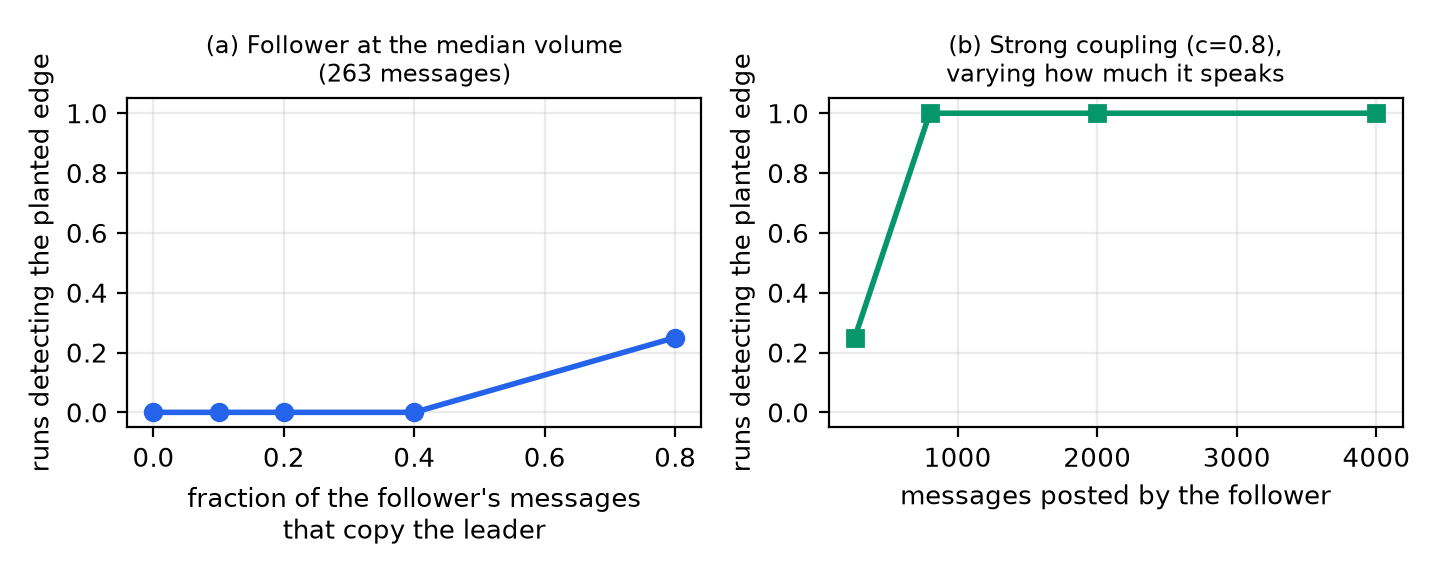
\includegraphics[width=0.92\textwidth]{f4_power.png}
\caption{Detection of a planted follower under the repaired surrogate. Left, varying the fraction of
its messages that copy the leader, at the median agent's volume. Right, varying how much it speaks,
at strong coupling.}
\end{figure}

\paragraph{Humans in the channel.} Main-village \#general is now effectively human-free, with 3 human
messages in the window, so the question has to be asked in open-chat, where 32\% of messages come
from 124 human visitors. Pairwise, with humans collapsed into one node, 19 edges are certified.
Conditioning removes almost all the agent-to-agent structure and little of the rest: \textbf{four
edges survive, of which three run from humans to agents, one is agent to agent, and none run from an
agent to a human.} The asymmetry is not an artifact of the confound. It should be read carefully all
the same: topical dependence from a person to an agent is also what ordinary responsiveness looks
like, so the measurement supports only that the dependence is dyad-specific and directional, not
that anyone is steering a swarm.

\section{Reproducibility, and one limitation of it}

Every number in this paper is recomputed from committed analysis output by a verifier that fails on a
mismatch, and that verifier covers the prose of this paper as well as the figures.

One limitation should be stated plainly. Re-running the counts in the earlier stationarity sweep with
the same seeds and configuration, only one of the eight cells reproduced exactly; the remaining
differences were one or two replicates per cell. Seven of the eight published rates still fell within
the recomputed Wilson intervals, and no conclusion changed. The exception is the zero-drift cell under
the permutation null, where the published 1 of 30 falls just below the recomputed interval of
$[0.035, 0.256]$ for 3 of 30, and no result here depends on that cell.

The generator, estimator and BLAS configuration were investigated and ruled out as the source. The
most likely explanation is a library-level difference, particularly in scikit-learn's $k$-means
implementation within the symboliser, whose output can vary between versions. Every sweep now records
the environment it ran under: Python 3.14.6, numpy 2.5.1, scipy 1.18.0 and scikit-learn 1.9.0,
including the BLAS build and the number of BLAS threads each worker used.

This does not make the previously published counts exactly reproducible. It provides a more clearly
specified environment in which subsequent results can be checked. For that reason I report rates
alongside their confidence intervals rather than exact replicate counts. The distinction between
reproducing a result within its uncertainty and reproducing every individual count matters, and only
the first is claimed.

\section{Conclusion}

Applied to real agent chat, the standard recipe for ``who drives whom'' needs repair before it says
anything. Clock windows cannot separate a message from its answer at the speed agents reply, and what
they certify is matched by a null with no access to meaning. The turn-ordered grid that fixes this
breaks the circular-shift surrogate: family-wise error 0.90 against a nominal 0.05, caused by the
speaker sequence itself. Restricted permutation surrogates repair most of that, but they are flat
under drift rather than calibrated, they are mutually indistinguishable at this precision, and one of
them needs twice the surrogate draws anyone would think to use. A valid surrogate fixes calibration
but not confounding. What survives is small: two dyad-specific edges that do not replicate, an
undetermined answer set by conditioning resolution, and influence running from people into agents and
never back. \textbf{An influence graph should not guide decisions until its error rate, its confound,
its detection floor and its symboliser's fidelity are reported.}

\section*{Limitations}

\begin{itemize}
\item \textbf{Immediate-predecessor only.} The turn-ordered lag-1 measure sees influence from the
message directly before a reply. Influence acting over several turns, or through a room's accumulated
context, is out of scope.
\item \textbf{Discrete approximation to an event process.} Agent chat is event-based in continuous
time. The turn-ordered discretisation with a permutation surrogate is a practical fix, and the
continuous-time comparison above shows what that choice gives up.
\item \textbf{The mechanism behind the real 0.90 is not established.} The generator separates
turn-taking from drift and points at drift, but the largest cell anywhere in the design is 0.365.
\item \textbf{Symbolisation quality cannot be measured on the real logs.} The central result survives
an independent symboliser, but the edge count does not: it moves with alphabet size and with which
messages the topic model is fit on. The floor remains the largest unquantified threat.
\item \textbf{No ground truth in the real logs.} The validity argument rests on planted controls and
on the meaning-free null, not on recovering a known answer.
\item \textbf{Conditioning removes real influence too.} The conditional estimate discards influence
that works by shifting what the channel is talking about, which in a group chat may be a large part
of genuine influence. It is a lower bound on dyadic influence.
\item \textbf{The human result is exploratory.} It rests on one village and one window and should be
read as a lead.
\end{itemize}

\section*{Broader impact and ethics}

This work audits influence detection on a population of AI agents, which is dual-use. Used
defensively it helps an overseer decide what an influence graph is worth, and the main result is
deflationary: it tells practitioners to trust these outputs less, which reduces rather than increases
the chance of acting on a bad attribution. The same tooling could be used to identify the most
influential agent in a swarm in order to target it, or to surveil participants in a channel. Three
properties limit the misuse. The subjects are AI models; the dataset is already public under research
terms and no re-identification is added; and the measure is weak and local, recovering
immediate-predecessor topical dependence rather than any model of how to steer an agent.

The dataset's research terms were followed: research use only, no training on the data, no
re-identification, citation of the source, and notification of the authors of resulting publications.
Human participants appear only as an aggregate node or as anonymised visitor labels, never by name or
handle, and no content attributable to an individual person is reported. Message text and metadata
were read, never model weights or private user data.

The use of a large language model in this work is disclosed in the first-page footnote, as TMLR
requires.

\bibliographystyle{tmlr}
\bibliography{refs}

\end{document}
"               camera-ready
% Use build.py, which runs all of them and checks the anonymous output for leaks.
\providecommand{\TMLRMODE}{submission}
\makeatletter
\def\@tmlrpreprint{preprint}
\def\@tmlraccepted{accepted}
\ifx\TMLRMODE\@tmlrpreprint
  \usepackage[preprint]{tmlr}
\else
  \ifx\TMLRMODE\@tmlraccepted
    \usepackage[accepted]{tmlr}
  \else
    \usepackage{tmlr}
  \fi
\fi
\makeatother

\usepackage{hyperref}
\usepackage{url}
\usepackage{booktabs}
\usepackage{graphicx}
\usepackage{amsmath}

% Gate every identifying string on whether identity may be revealed at all. The flag to test is
% \if@accepted, NOT \if@preprint: tmlr.sty's [preprint] option sets BOTH, so \if@accepted is true
% for the preprint and the camera-ready and false only for the anonymous submission, which is
% exactly the condition wanted. Gating on \if@preprint alone also hid the repository URLs from the
% camera-ready, which is where this paper promises to give them. \if@accepted is internal to
% tmlr.sty, hence the \makeatletter. The anonymous build takes the second argument.
\makeatletter
\newcommand{\ifdeanon}[2]{\if@accepted#1\else#2\fi}
\makeatother
\newcommand{\benchname}{\ifdeanon{SwarmInfluence-Bench}{the benchmark}}

% An unmarked footnote, for the LLM-use disclosure. TMLR's FAQ requires the disclosure and names
% the location: authors must "mention explicitly in their submission that they have used this
% tool", "as a footnote on the first page". Verified against jmlr.org/tmlr/faq.html on 10 Nov 2026.
% It is therefore not optional, and it does not belong in Broader Impact, where it sat until now.
% Nothing in the policy asks for the vendor's name, so none is given.
\newcommand{\disclosurefootnote}[1]{%
  \begingroup\renewcommand\thefootnote{}\footnote{#1}\addtocounter{footnote}{-1}\endgroup}

\title{An Influence Graph Over AI Agents Certifies an Agent That Copies Nobody}

% Hidden by the tmlr package unless [accepted] or [preprint] is given.
\author{\name Manu Nicholas Jacob \email manunicholasjacob@gmail.com \\
        \addr Independent Researcher}

\def\month{11}
\def\year{2026}
\def\openreview{\url{https://openreview.net/forum?id=XXXXXXXXXX}}

\begin{document}
\maketitle

\begin{abstract}
Circular-shift surrogates can produce severely inflated false-positive rates when applied to
turn-ordered multi-agent conversations, reaching a family-wise error rate of 0.90 against a nominal
0.05. A generated benchmark separates two candidate mechanisms and points at non-stationary speaker
activity rather than turn-taking, which suppresses the failure rather than causing it. No setting of
either knob reproduces the observed 0.90, however, so what drives the full real-data failure remains
open. Restricted permutation surrogates substantially reduce the problem. Their error rate is flat
with respect to drift rather than at the nominal level, and for the global within-speaker variant it
depends on how many surrogate draws the null is built from. Calibration alone does not address
confounding, which motivates a conditional estimator validated against a benchmark with planted
ground truth. I also identify a symbolisation-dependent detection limit and develop label-free
diagnostics for it, and show that their calibration does not transport across degradation
mechanisms. The benchmark is released.
\end{abstract}

\disclosurefootnote{\textbf{Use of a large language model.} A large language model was used as an
assistive tool: to help write and run the analysis code, and to help draft this paper. The author is
responsible for every claim, number and figure. All results come from the released code run on the
public dataset, no result or reference is fabricated, and every number in this paper is recomputed
from committed analysis output by a verifier that fails the build on a mismatch.}

\section{Introduction}

When AI agents interact in a shared channel, it is useful to understand how they influence one
another. Information-theoretic methods offer a way to measure this through lagged transfer entropy,
surrogate testing, and per-agent influence scores. They are attractive because they require no
labels and no access to model internals, only a record of who said what and when. The reliability of
those measurements is what this paper examines.

Almost every demonstration of these detectors runs on synthetic traces with a planted leader, where
the analyst controls timing and vocabulary. Real agent chat is asynchronous, bursty, and written in
open language. The narrower question here is whether the standard recipe, applied to real agent
logs, returns anything an overseer should act on.

The audit runs on the AI Village corpus \citep{aidigest2026}, in which frontier models share chat
channels over eighteen months across four villages differing in size, lifetime and tempo, applying
the checks a reader should demand: planted controls, a meaning-free symboliser, replication in a
held-out window, and sensitivity to every parameter that had to be chosen.

\begin{enumerate}
\item The conventional circular-shift surrogate is \textbf{invalid} on turn-ordered agent chat: a
family-wise error rate of 0.90 against a nominal 0.05, caused by the structure of the speaker
sequence itself.
\item Restricted permutation surrogates restore most of the calibration, and re-certifying under one
\textbf{scrambles rather than shrinks} the answer: one channel loses all 11 of its edges, another
gains 15.
\item The three restricted variants are \textbf{mutually indistinguishable} at the precision reached
here, so the choice between them cannot be justified on error rate. The global within-speaker
variant additionally needs on the order of 200 surrogate draws, and over-fires by roughly a factor
of two at 100.
\item Calibration is not confounding, so a conditional estimate is added and validated on a released
benchmark with a known influence graph: common-cause false edges fall from 22.3 to 0.33, and on the
planted-edge instances precision rises from 0.17 to 0.80 with no loss of recall or power.
\item The same benchmark exposes a \textbf{symbolisation floor}. Below roughly 0.44 adjusted Rand
index between symboliser and truth, detection collapses whatever the estimator. Label-free
diagnostics detect that floor, but their calibration does not transport across degradation
mechanisms, and I report where it fails.
\item On the real channels two edges stand at every conditioning resolution, 18 are
\textbf{undetermined} between 0 and 13, none replicates out of sample, and what survives alongside
humans runs from people to agents.
\end{enumerate}

\section{Related work}

\paragraph{Transfer entropy and surrogates.} Transfer entropy \citep{schreiber2000} measures how much
a source's past reduces uncertainty about a target's next symbol beyond the target's own past.
Plug-in estimators are biased upward on short series, so significance rests on surrogate data, with
family-wise error controlled by a max-T test \citep{westfall1993}. The usual surrogate is a circular
time shift of the source.

\paragraph{Event-based data breaks the shift surrogate.} \citet{shorten2021}, on neural spike trains,
show that the conventional source-time-shift surrogate fails to represent the null hypothesis of
conditional independence for event-based processes, and adapt to that setting the nearest-neighbour
local permutation scheme of \citet{runge2018}. Agent chat is event-based in that sense: messages are
events in continuous time, not samples of a clocked signal. The correction is not a contribution of
this paper. The contribution is showing that the same failure carries over to multi-agent safety
monitoring, and that it can be severe enough to create apparent leaders where none exist.

\paragraph{The same failure, concurrently, in multi-agent reinforcement learning.}
\citet{papadopoulos2026} report a closely related surrogate failure in multi-agent
reinforcement-learning action series. Their agent pairs have zero influence by construction, yet
circular time shifts produce false-positive rates of 100\% and 98.2\% against a nominal 0.05. A
plain permutation surrogate fares no better in their setting, at 100.00\% and 99.95\%. Their
proposed correction restricts permutations to blocks of training time, which returns the rates to
5.25\% and 5.50\%.

There are important differences between their setting and this one. Their data consist of binary
actions recorded over twelve thousand training rounds, whereas these data are symbolised
natural-language messages arranged on a turn-ordered conversational grid. Their non-stationarity
comes from monotone drift associated with annealing exploration; here the relevant non-stationarity
appears in the speaker sequence. Neither result should be taken as a direct extension of the other.

Nevertheless, the fact that both approaches rely on restricted permutations is worth noting. Their
permutation blocks are defined by training time, while mine are defined by an agent's own speaking
positions. This provides convergent evidence that unrestricted temporal rearrangement can be
problematic in non-stationary multi-agent data. Their findings also serve as a useful warning for
the approach taken here, and the warning has a measured form rather than a rhetorical one: in their
data the unrestricted permutation failed as completely as the time shift, at 100.00\% against a
nominal 0.05. Permutation-based surrogates are not automatically protected against
non-stationarity, and what protects the one used here is the restriction, not the permutation. I
claim no priority over their result and view the two studies as complementary, addressing different
forms of structured multi-agent data.

\paragraph{Oversight under a budget.} AI-control research frames monitoring as resource constrained,
with a cost for false positives \citep{greenblatt2024}. An influence graph is one such measurement,
and its error rate is the concern here.

\paragraph{Clustering stability.} The idea of using clustering stability as a label-free quality
indicator is not new. It has a substantial history, including \citet{benhur2002},
\citet{lange2004}, von Luxburg's review of clustering stability \citep{vonluxburg2010}, and
\citet{tibshirani2005} on prediction strength. What is different in Section~\ref{sec:floor} is the
calibration of these diagnostics against a detection-performance floor rather than against cluster
recovery alone.

\section{Data and representation}

The AI Village dataset ships one gzipped-JSONL table per village. Four villages are used, differing
enough to test whether any finding is a property of one channel.

\begin{table}[h]
\centering
\begin{tabular}{lrrrrl}
\toprule
village & agent messages & agents & lifetime & human messages & busiest room \\
\midrule
main      & 205,726 & 58  & 576 days & 10,029 & \#general (166,715, 81\%) \\
open-chat &  35,483 & 23  &  66 days & 12,264 & \#general (all) \\
swarm     &   3,848 & 133 &   1 day  &      5 & room a (3,846) \\
game-jam  &     838 & 6   &   3 days &     36 & per-team rooms \\
\bottomrule
\end{tabular}
\caption{The four villages. A 2026 scaffolding change scopes each agent to its current room's
context, so the busiest room of each village is a self-contained influence substrate and is analysed
alone.}
\end{table}

The primary window is the final fourteen days of main-village \#general, 17 to 31 October 2026,
holding 8,800 agent messages. Twenty-two models posted at least 50 messages each and the directed
test uses the 15 busiest, giving 7,958 message events. Two scaffolding facts are disclosed rather
than corrected: the automated nudger was off throughout, and the unused \#best and \#rest rooms were
soft-deleted mid-window, which does not touch \#general.

\subsection{From open language to symbols}

Transfer entropy needs discrete symbols, so each message is mapped to a small alphabet before
influence is estimated, and that mapping is kept separate from the estimator. A topic symboliser
(TF-IDF then $k$-means, $k=8$) gives a message its topic cluster id, so paraphrases of one idea share
a symbol. A hash symboliser, a stable hash of the normalised text into $k=8$ buckets, has no notion
of meaning and serves as a null: an edge appearing under both lives in timing alone.

\subsection{The lag problem, and why clock windows cannot solve it}

A lag-1 transfer entropy compares window $t-1$ with window $t$, so influence landing inside one
window is invisible to it. Agent chat makes this binding. Among the fifteen analysed agents the gap
between consecutive messages by different speakers has a median of 28.1 seconds (25th percentile
9.2, 75th 66.2, 95th 159.3), so turn-taking is a seconds-scale process while any clock window wide
enough to hold two speakers is minutes wide and swallows both a message and its answer.

Both horns are measurable. At 30 seconds only 1.2\% of agent-windows hold a message, while 32.0\% of
replies already land in the same window as what they answer, rising to 84.4\% at five minutes. At
every width tried, the meaning-free hash null certifies comparably many edges, and more at five
minutes: 9 against 12 at thirty seconds, 17 against 19 at one minute, 27 against 44 at fifteen, and
19 against 17 at five. Whatever clock-window transfer entropy was detecting there, it was not shared
meaning.

\begin{figure}[h]
\centering
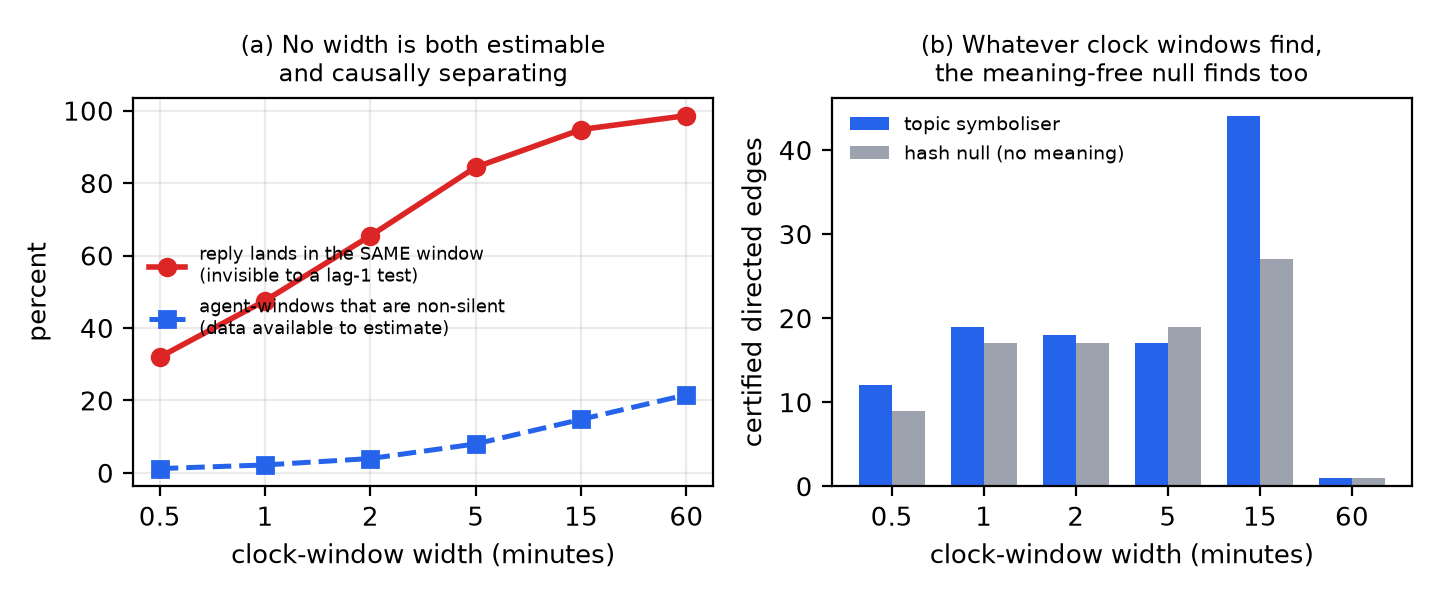
\includegraphics[width=0.92\textwidth]{f1_clock.png}
\caption{Clock-window transfer entropy on the 15 analysed agents of main-village \#general. Left,
the two failure modes as a function of window width. Right, edges certified under the topic
symboliser against the meaning-free hash null.}
\end{figure}

The bind is avoided by ordering messages canonically and letting one message be one tick. Each
agent's series carries its symbol where it spoke and a silent symbol elsewhere, so the lag-1
comparison is between a message and the one immediately before it. The cost is that the measure
captures immediate-predecessor influence only.

\section{The surrogate failure, and two explanations that did not hold}
\label{sec:failure}

An agent is planted into the real stream, drawing its symbols from the channel's marginal and
coupled to nothing at all. It is certified as driving something in 3 of 8 runs when it posts 50
messages, and in 8 of 8 at 100, 263, 600 and 1500 messages, with the mean largest $z$ rising from 5.6
to 12.3, 21.7, 38.3 and 71.7. The error grows with how much the agent speaks, which rules out a
small-sample explanation.

A planted agent could be dismissed as artificial, so the error rate is also measured directly.
Keeping the real speaker sequence and permuting the symbols globally leaves data with no directed
topical influence by construction. The shift surrogate certifies at least one edge in 9 of 10 such
replicates, a family-wise error rate of 0.90 against a nominal 0.05.

\paragraph{What breaks it is the speaker sequence.} Destroying one structure at a time isolates the
cause. Keeping the real speaker order and shuffling only symbols, the shift surrogate fires in 10 of
10 replicates; randomising the speaker order as well drops it to 0 of 10; uniform symbols with the
real order still give 6 of 10. So the driver is the structure of the speaker sequence, not the
symbol distribution and not sparsity. That sequence is far from random in two ways at once: it
repeats a speaker 36\% of the time and returns after one message 38\% of the time, and each agent's
activity is strongly non-stationary, with a median block-share coefficient of variation of 0.79.
Shuffling the order destroys both at once, so this ablation cannot say which of the two mattered.

\subsection{Two explanations I proposed, and the benchmark refuted both}

I initially attributed the failure to mutual exclusivity: only one agent can speak at each tick, so
shifting individual timelines could create overlaps that never occurred in the original
conversation. The benchmark did not support this explanation. A generated channel with exactly one
speaker per tick and steady activity produced an error rate of just 0.025, 95\% Wilson
$[0.011, 0.057]$, far below the 0.90 observed in the real data. Mutual exclusivity alone therefore
cannot explain the failure.

I then suspected turn-taking. In the real channel, speakers repeat 36\% of the time and return after
exactly one message 38\% of the time. However, adding a Markov speaker chain to the generator
produced the opposite result. Turn-taking suppressed the error rather than increasing it. At the
nominal knob values and with no drift the surrogate certified nothing at all across 200 replicates,
while removing turn-taking and introducing drift raised the rate to 0.365. The contribution from
drift was $+0.340$, compared with $-0.025$ for turn-taking. The same inversion appears in the arm
calibrated so that the generated channel reproduces the real channel's measured repeat, return and
block-share statistics rather than merely carrying those numbers as settings: there, turn-taking
alone also certifies nothing, and drift alone gives 0.065.

Neither mechanism, nor their combination in the tested design, reproduced the real-data error rate of
0.90. The largest cell anywhere in the design is 0.365. The real-data ablation removes turn-taking
and non-stationarity together, while the generator separates them. The results point to
non-stationary activity, but the remaining gap means the mechanism behind the full real-data failure
is not yet established.

Every figure above comes from the run at 200 surrogate draws. The first version of this analysis
used 100, which inflates both nulls on the same 2,400 instances: the circular shift fires 53 times
where the 200-draw run does not, against 18 the other way (exact McNemar $p = 3.9 \times 10^{-5}$),
and the permutation surrogate 83 against 20 ($p = 2.7 \times 10^{-10}$). Every qualitative conclusion
in this section is the same at both settings, which is why they are worth stating at all. The
numbers are not, so the draw count belongs in the caption.

\section{The repair, compared}
\label{sec:repair}

Following the local-permutation idea of \citet{runge2018} as adapted by \citet{shorten2021}, each
source keeps its speaking positions and only its symbols are permuted among them. Speaking pattern,
sparsity and turn-taking are preserved exactly, and only the correspondence between symbol and time
is destroyed. On the same destroyed-structure real data the family-wise error rate falls to 0.063
over 300 replicates, 95\% Wilson $[0.041, 0.097]$. The planted uncoupled agent is never certified: 0
of 5 at both 263 and 1500 messages, with mean max $z$ of 2.8 in each case against 22.0 and 68.3
under the shift surrogate.

\begin{figure}[h]
\centering
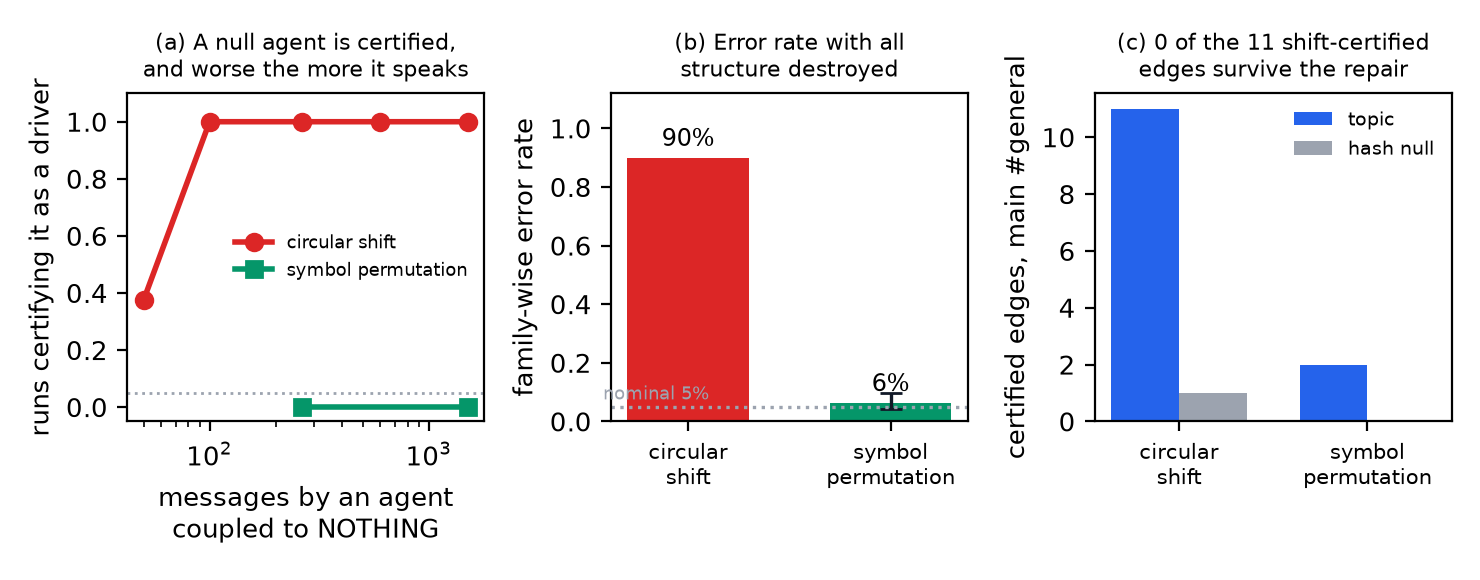
\includegraphics[width=\textwidth]{f2_null.png}
\caption{Left, how often an agent coupled to nothing is certified as a driver, under each surrogate.
Middle, family-wise error rate measured on data with all structure destroyed, with a Wilson
interval; the dotted line is the nominal 0.05. Right, what each surrogate certifies on the real
channel.}
\end{figure}

\subsection{How many surrogate draws are needed}

The number of surrogate draws matters more than I initially appreciated. In a paired comparison of
300 instances, where all four surrogates run on identical symbol grids so the outcomes are paired,
the global permutation surrogate produced a false-positive rate of 0.1167 with 100 draws, falling to
0.0700 with 200 draws, 95\% Wilson $[0.046, 0.105]$. This difference is statistically significant
(exact McNemar $p = 0.0043$). The block-local and Runge local permutations were less sensitive to the
increase: their corresponding rates changed from 0.0900 to 0.0767 and from 0.0967 to 0.0800.

At 200 draws, the global permutation's interval covers the nominal 0.05 and overlaps the real-data
estimate of 0.0633 $[0.0409, 0.0968]$. The real-data result is therefore corroborated rather than
overstated. For practical use, the important point is that reducing the number of surrogate draws
can materially change the result. In particular, the global permutation over-fires at 100 draws by
approximately a factor of two. I would therefore not treat the choice of draw count as a minor
computational detail.

The same correction applies to the benchmark-wide estimate. That figure was 0.0942 at 100 draws.
Repeating all 2,400 instances at 200 draws gives \textbf{0.0679}, 95\% Wilson $[0.0585, 0.0787]$,
and the paired difference is large: 83 instances fire at 100 draws and not at 200, against 20 the
other way, $p = 2.7 \times 10^{-10}$. The conclusion it supports is unchanged, because the interval
still excludes the nominal 0.05. So the permutation repair does carry a residual inflation on clean
generated data, but it is about a third above nominal rather than nearly double.

One limit on this recommendation. I compared 100 draws against 200 and did not test any larger
value, so what the experiment establishes is that 100 is too few, not that 200 is enough. Two
hundred is a lower bound on the draw count rather than a converged setting, and a practitioner whose
conclusions sit near a decision boundary should check their own sensitivity rather than adopt the
number.

\subsection{Choosing a repair, when the error rate cannot choose}

The comparison of the three permutation-based repairs does not produce a clear winner. All four
surrogates were evaluated on identical symbol grids across 300 pure-null replicates, so the
comparison reflects differences between the null models rather than differences between datasets.

\begin{table}[h]
\centering
\begin{tabular}{lrrrl}
\toprule
surrogate & FWER, 100 draws & FWER, 200 draws & 95\% Wilson at 200 & nominal 0.05 \\
\midrule
circular shift                   & 0.0433 & \textbf{0.0333} & $[0.018, 0.060]$ & inside \\
global within-speaker permutation & 0.1167 & \textbf{0.0700} & $[0.046, 0.105]$ & inside \\
block-local permutation          & 0.0900 & \textbf{0.0767} & $[0.052, 0.112]$ & excluded \\
local permutation \citep{runge2018} & 0.0967 & \textbf{0.0800} & $[0.054, 0.116]$ & excluded \\
\bottomrule
\end{tabular}
\caption{Four surrogates on identical symbol grids, 300 pure-null replicates, at both draw counts.}
\end{table}

At 200 draws, paired on the same 300 instances, the circular shift is not significantly different
from the global permutation ($p = 0.0614$), although it differs from block-local permutation
($p = 0.0294$) and from Runge's local permutation ($p = 0.0201$). At 100 draws it differed from all
three, which is the draw-count artifact again. The three repairs remain statistically
indistinguishable from one another, with pairwise $p$-values of 0.85, 0.65 and 1.00. The apparent
differences in their error rates are not sufficient to establish a ranking.

Choosing between them therefore requires more than calibration, and two readings pull against each
other. Runge's local permutation has the strongest methodological justification for preserving the
structure it is intended to preserve, and it follows the approach adapted to event data by
\citet{shorten2021}. Block-local permutation is more heuristic and introduces a free parameter that
has not been tuned. Global permutation is the simplest. On the other hand, the global permutation has
the most favourable interval relative to the nominal rate, and is the only repair that costs nothing
measurable against the shift on clean stationary data, although neither difference is statistically
established. I do not consider the observed error rates sufficient to select one repair over the
others. The choice should be guided by the structure the null is intended to preserve and the
assumptions that can be justified for the data.

\subsection{When to use the repair}

A drift sweep gives the practical reading. Across 150 replicates per cell at 200 surrogate draws,
the circular shift degrades steadily as activity drift increases while the three repairs do not.

\begin{table}[h]
\centering
\begin{tabular}{lrrrr}
\toprule
activity drift & circular shift & global permutation & block-local & local \\
\midrule
0.0 & \textbf{0.013} & 0.093 & 0.080 & 0.093 \\
0.3 & 0.100 & 0.100 & 0.093 & 0.120 \\
0.6 & \textbf{0.193} & 0.053 & 0.047 & 0.067 \\
0.9 & \textbf{0.380} & 0.087 & 0.080 & 0.080 \\
\bottomrule
\end{tabular}
\caption{Family-wise error on pure nulls as activity drift increases, 150 replicates per cell, 200
surrogate draws. Every certified edge is a false positive by construction.}
\end{table}

The pattern is supported by a formal trend test rather than by eye. A Cochran-Armitage test across
the four ordered drift levels gives the circular shift $z = 8.667$, $p < 10^{-15}$, and gives every
repair nothing: $p = 0.51$ for the global permutation, 0.63 for block-local and 0.37 for local. The
same pattern holds at both surrogate draw counts, so it does not depend on that choice.

The repairs are therefore flat under drift rather than calibrated. Only one of the four global
permutation intervals covers the nominal 0.05, and the rest sit nearer 0.09, so what the repair buys
is insensitivity to drift rather than correctness. One asymmetry should be stated rather than
hidden: block-local covers nominal in three of the four cells where the global repair covers one.
The two remain pairwise indistinguishable, so this is not grounds to switch the recommendation, but
it does mean the global repair cannot be described as the best-calibrated under drift.

The results also show why the repair should not be treated as universally preferable. At zero drift
the circular shift has an error rate of 0.013, while the three repairs are all around 0.08 to 0.09.
That advantage is gone by the first drift step: at drift 0.3 the shift reads 0.100 against the global
permutation's 0.100 and block-local's 0.093, so the crossover falls between drift 0.0 and 0.3 rather
than at some higher level. By drift 0.6 the shift is roughly four times the repairs. If a channel has
been checked and found stationary, the circular shift may be sufficient. When activity is
non-stationary the repairs are the more stable choice, and the margin for error on that judgement is
narrow, because the crossover arrives by the first drift level tested.

\section{Continuous time, and what the repair cannot test}

An earlier analysis identified continuous-time estimation as the principled option for event data
but did not evaluate it. Running the continuous-time estimator CoTETE on both channels certifies 0
edges in either case, compared with 2 for main-village and 18 for open-chat under the discrete,
turn-ordered analysis. Its highest $z$-scores are 3.062 and 3.980, below the respective max-T
thresholds of 4.171 and 4.308.

At first these results might appear to contradict the symbol-based analysis. The two estimators
operate on different information, however. CoTETE's public API takes event times with no symbol
channel, while the transfer-entropy analysis here uses topic symbols. To test whether this
difference explains the results, I reduced the data to timing alone, replacing every spoken symbol
with the same code. Under this representation the estimator used here also detects 0 edges in both
channels, matching CoTETE. Using the circular-shift surrogate instead produces 12 and 3 edges. So
neither method detects relationships from event timing alone in these channels, and the edges found
by the symbol-based analysis depend on symbol correspondence, which the continuous-time estimator
cannot access.

Two caveats attach to those $z$-scores, and the second attaches to the larger of them. Point
estimates from this estimator are stochastic to about 17\% across repeated runs, so none of these
values should be read to more than two significant figures. And open-chat's highest $z$, the 3.980,
belongs to the one pair whose surrogate draws mostly failed: it needed 1,936 failed draws to obtain
100 successes, a 4.9\% success rate. Those surrogates are conditioned on being estimable, so that
pair's null is biased in an unknown direction. The conclusion does not rest on it, since that pair
falls below threshold and so does every other pair, but the number should not be quoted as a clean
measurement. The failures themselves were a defect rather than a property of the data: an enlarged
exclusion window can empty the neighbour search on sparse bursty event trains and raise an error
that terminates a whole pair, with no handling at the public entry point. This has been reported
upstream.

There is also a fundamental limitation in applying the recommended permutation surrogate to
timing-only data. When every event carries the same symbol, permuting those symbols changes nothing.
The observed statistic and the surrogate null are identical, making the test exactly degenerate:
standard deviation 0 across all 210 pairs and $p = 1.0$ everywhere. \textbf{The repair has zero power
against timing structure by construction.} The permutation surrogate is appropriate for testing
relationships in the symbol sequence, but it does not answer whether relationships exist in event
timing. These are different questions, and choosing one null means giving up the ability to test the
other with that procedure.

\section{Confounding, and what conditioning removes}

A valid surrogate fixes calibration but not confounding. If every agent tracks a drifting channel
topic, every pair is genuinely dependent through the channel, and pairwise transfer entropy cannot
tell that from direct influence. I therefore also report a \textbf{conditional} estimate, which asks
whether a source's last message adds anything about a target's next one beyond the target's own
history and the channel's recent state. The conditioning variable is the modal symbol of the last
twelve messages, excluding the immediately preceding one so that it does not simply restate the
source.

On a generated benchmark whose decisive instances contain no influence while every agent tracks a
shared drifting topic, so that any certified edge is common cause, pairwise transfer entropy
certifies \textbf{22.3} edges on average and conditioning takes that to \textbf{0.33}, lifting pooled
precision on the four-edge instances from 0.17 to \textbf{0.80} at a recall of 1.0 either way. Across
couplings from 0.05 to 0.8 the conditional test still finds the planted edge in 3 of 3 runs, so the
gain costs no power.

The benchmark flatters the conditional estimator, since its common cause is a shared modal topic and
the conditioning variable is the channel's modal topic. The real channels are harder, and
conditioning there costs degrees of freedom: a 9-symbol alphabet with a 9-valued context gives 6,561
cells against about 7,900 ticks, so that variable is also coarsened to 4 and 2 values.

\begin{table}[h]
\centering
\begin{tabular}{lrrrr}
\toprule
channel & pairwise & conditional, 9 values & 4 values & 2 values \\
\midrule
main \#general      & 2  & \textbf{2, the same two edges} & 2 & 3 \\
open-chat \#general & 18 & \textbf{0} & \textbf{7} & \textbf{13} \\
swarm, room a       & 1  & \textbf{0} & & \\
\bottomrule
\end{tabular}
\caption{Conditioning at three resolutions. Main-village's two edges are robust to that choice;
open-chat's zero is not.}
\end{table}

At the finest resolution the open-chat test is degenerate, its surrogate sitting above the observed
statistic for 65\% of pairs with the largest $z$ in the family only 4.4, so it is failing to reject
rather than finding nothing to reject. Open-chat's structure therefore remains
\textbf{undetermined}: depending on the conditioning resolution, between 0 and 13 of its 18 edges may
survive. That resolution is a free parameter an analyst would set once and never revisit. This is a
property of the channel rather than the estimator: on structure-free real data the conditional test
fires in 2 of 40 replicates, an error rate of 0.05 with a mean $z$ of $-0.001$, so it is nominal
rather than conservative.

\section{The symbolisation floor}
\label{sec:floor}

Everything these methods produce is downstream of turning text into symbols. On the benchmark, where
the underlying topics are known, detection performance drops sharply when agreement between the
symboliser and the ground truth falls below roughly ARI 0.44, and this behaviour appears across the
tested estimators. Importantly, the false-positive rate can look \emph{better} below this point,
because the shared topic structure needed to produce confounded detections is no longer represented
reliably. A pipeline that stops detecting relationships may therefore have lost the signal it needs
rather than become more reliable, and nothing downstream of the symboliser can tell those apart.

\subsection{Detecting the floor without labels}

That degradation can be detected without ground-truth labels. Across the nine-level benchmark sweep,
three statistics separate the below-floor cases with zero errors: seed stability at a threshold of
0.623, agreement with LSA at 0.646, and the Calinski-Harabasz index at 138.9. Seed stability here is
the \textbf{minimum} pairwise agreement across seeds, not the mean; the mean variant makes one error,
at a different threshold of 0.791. Silhouette has the strongest correlation with true ARI, at 0.979,
but is not useful for identifying the boundary because its threshold falls within a gap of just
0.002. A statistic that tracks clustering quality most closely is not necessarily the best one for
making a classification decision.

Error count cannot choose among the three that were perfect, so I tested whether each threshold still
means what it meant when the channel changes for reasons other than topic separability. Applying each
cut unchanged to thirty cells that vary turn-taking, drift, agent count, volume skew, message length
and corpus size, twenty-seven of which hold true ARI at exactly 1.000:

\begin{table}[h]
\centering
\begin{tabular}{lrrrr}
\toprule
diagnostic & cut & errors where fitted & errors, nuisance set & of those at true ARI 1.000 \\
\midrule
seed stability, min across seeds & 0.623 & 0 & 2 & \textbf{0} \\
LSA agreement                    & 0.646 & 0 & 2 & \textbf{0} \\
Calinski-Harabasz                & 138.9 & 0 & 6 & \textbf{3} \\
\bottomrule
\end{tabular}
\caption{Whether a cut fitted on the vocabulary-overlap mechanism survives a change in the channel
that is not a change in topic separability.}
\end{table}

The two bounded statistics err only on the short-message cells, where the symbolisation genuinely has
degraded. Calinski-Harabasz additionally condemns all three cells whose true ARI is exactly 1.000,
for no reason beyond the corpus holding 2,000 messages rather than 8,000, where it reads 76 to 77
against its own cut of 138.9. It is unbounded and grows with sample size, so a published numeric
threshold for it carries no meaning on another corpus. That is why I recommend the two bounded
statistics and not the index that matched them on error count. \textbf{A cut that moves with the
corpus is not a floor cut.}

This is not a weak statistic being discarded on a technicality. Calinski-Harabasz correlates with
true ARI at 0.973, almost as closely as silhouette, and unlike silhouette it classifies the floor
perfectly where it was fitted. It still cannot carry a published threshold. That is the sharper form
of the point above: neither the statistic that tracks quality most closely nor the one that
classifies best on the fitting mechanism is necessarily the one whose cut another researcher can
reuse.

There are important limits to this result. The effective sample size is nine rather than 54, because
the classification label is determined by overlap level. There are no observations between ARI 0.444
and 0.222, so the exact location of the boundary within that interval remains unknown. These
diagnostics classify whether a result is below the tested detection floor; they do not estimate ARI,
and their behaviour is flat between 0.68 and 1.00, and not even monotone there. The benchmark also
uses a single degradation mechanism with a known and correct value of $k$, whereas the true number of
topics in real conversations is unknown. I therefore treat 0.44 as a benchmark-specific, bracketed
result rather than a universal threshold.

\subsection{A contradiction the diagnostic lost}

I initially used these diagnostics to classify one real channel, open-chat, as below the
symbolisation floor. That conclusion did not agree with the channel's measured results: open-chat
certified 18 and 22 edges under the two symbolisers, compared with 2 and 1 for main-village, and its
hash-based null certified zero edges. Rather than treating this disagreement as evidence that the
original measurements were wrong, I revisited the diagnostic itself.

The problem was the choice of $k$. Repeating the comparison with the same channels, loader and window
reproduced the published $k=8$ results to the digit. At $k=4$, however, open-chat reached stability
scores of 0.950 and 0.978, the highest values produced by either channel across the tested settings,
and both exceeded the diagnostic thresholds. The earlier below-floor classification was therefore a
conclusion about one arbitrary choice of $k$, not a reliable statement about the channel. Message
length does not explain the difference either: 27.1\% of main-village messages contain fewer than
five tokens, compared with 2.3\% in open-chat, so the short-message channel is the one the diagnostic
cleared.

This correction changes how the symbolisation results should be read, and it withdrew three claims.

\begin{enumerate}
\item \textbf{The claim that no topic signal remains below the floor is too strong.} The
circular-shift surrogate recovers all four planted edges at every tested overlap level, including
0.95, where ARI is 0.011. The observed collapse is in the permutation null, not necessarily in the
underlying data.
\item \textbf{ARI 0.44 cannot be treated as a universal detection threshold.} When the shared-topic
parameter is 0, detection continues down to ARI 0.296, so the boundary depends on both the
symboliser and the channel.
\item \textbf{Edge counts cannot be used as a measure of symboliser quality.} Even at ARI exactly
1.000, changing the shared-topic parameter alone moves the permutation edge count from 5 to 78.
\end{enumerate}

The diagnostics also do not transfer reliably outside the mechanism on which they were evaluated.
Their balanced accuracy falls from 1.00 to 0.75 and 0.571 under a known mismatch in $k$. All seven
errors made by seed stability are false below-floor classifications, and in every one of those cases
the detector still identifies all planted edges; of the fourteen cells it condemned, eleven had full
conditional recall. The failure direction is the dangerous one: it condemns working symbolisations.

This was an important correction to my own interpretation. I introduced a diagnostic to check whether
the symbolisation was reliable, applied it to the real channels, and found that it contradicted
measurements already in hand. Investigating that contradiction showed the diagnostic was sensitive to
an arbitrary modelling choice. The result is not that the original measurements were wrong, but that
the control was being asked to support a broader conclusion than the evidence allowed. These
diagnostics remain useful within their tested setting, and \textbf{no channel-level floor verdict
should be issued from a single $k$}.

\section{The benchmark}

Real logs have no ground truth, so the common-cause question could not be settled on them. The
generator used here makes the influence graph known by construction: it decides, in code, who speaks
at which tick, on which topic, and who reacts to whom. Surface text is a separate, replaceable layer
drawn from disjoint per-topic vocabularies, so the whole thing runs offline and a detector still has
to symbolise raw text rather than read the labels. Turn-taking and activity drift are independent
knobs, so the two can be varied one at a time, and the generator reproduces its earlier behaviour
bit for bit when both are zero.

\benchname{} is released with 150 tests covering the generator, the detector harness, the text layer,
the floor analysis and the turn-taking factorial.
\ifdeanon{Code and benchmark:
\url{https://github.com/manunicholasjacob/swarm-influence-bench} and
\url{https://github.com/manunicholasjacob/swarm-influence-audit}.}{Code and benchmark are publicly
released; the links are withheld here for anonymity and will be given in the camera-ready version.}

One property of the benchmark must be stated when its numbers are quoted. Planting an edge displaces
other agents' speaking turns, so the generated instances contain real lag-1 dependencies that the
label set does not list. Precision measured against those labels is therefore a \textbf{lower bound}
for any detector, and what the benchmark supports is the comparison between two estimators rather
than the absolute value of either.

\section{What an overseer should do}

Six inexpensive controls should be included whenever an influence graph over an agent channel is
published.

\begin{enumerate}
\item \textbf{Plant an agent coupled to nothing, at your channel's volumes, and check it is not
certified.} This one test would have caught the failure reported here, at one run per volume.
\item \textbf{Measure the error rate directly}, by destroying the structure your method claims to
find and checking the family-wise rate is near nominal. If it is not, your surrogate does not match
your data.
\item \textbf{Preserve the speaker sequence in your surrogate.} Any surrogate that moves an agent's
messages in time will disturb it, and \citet{shorten2021} is the principled route. Use at least 200
surrogate draws, because at 100 the global within-speaker permutation over-fires by roughly a factor
of two.
\item \textbf{Establish the detection floor before interpreting an absence.} ``No edges'' and ``no
influence'' are different claims.
\item \textbf{Condition on the channel, report both numbers, and sweep the resolution.} Pairwise and
conditional bound the answer, and the gap between them is the result. Conditioning costs cells, so
check whether your answer is an artifact of how finely you conditioned. On one channel here it was.
\item \textbf{Report how well your symboliser agrees with the truth, on data where you know it.}
Everything is downstream of turning text into symbols, and below roughly ARI 0.44 detection
collapses whatever the estimator. I have found this control in no influence-detection paper, and it
is also the one that cannot be run on real logs, which is why the floor remains the largest
unquantified threat here.
\end{enumerate}

Two habits follow: publish a meaning-free null's count beside the real one, and require held-out
replication before calling a graph a structure.

\section{The real channels, and what survives}

Re-running every channel under the repaired surrogate changes the answers, and not in one direction.

\begin{table}[h]
\centering
\begin{tabular}{lrrr}
\toprule
channel & window messages & shift: topic / hash & permutation: topic / hash \\
\midrule
main \#general      & 8,800 & 11 / 1 & 2 / 0 \\
open-chat \#general & 8,226 & 3 / 0  & 18 / 0 \\
swarm, room a       & 3,846 & 2 / 1  & 1 / 0 \\
\bottomrule
\end{tabular}
\caption{The same channels under both surrogates, with the meaning-free hash null beside each.}
\end{table}

In main-village, \textbf{none} of the 11 edges the standard recipe certifies survives the repair, and
the two the valid surrogate certifies were not among them. In open-chat the correction runs the other
way, 3 edges becoming 18, because pathological pairs inflate the max-T threshold and raise the bar
for everything else. An invalid surrogate does not simply add false positives; it scrambles the
result.

Main-village's two edges are the strongest thing here and they are still not a finding, because they
do not replicate: the adjacent fourteen-day window certifies nothing at all under either estimator.
Given the detection floor, that silence is as consistent with the test sitting near its limit as with
the edges being absent, and the two cannot be separated. Power is governed by how much an agent says
as much as by how strongly it copies, and it is channel-specific: in main-village a planted follower
copying on 80\% of its messages is caught only 1 time in 4, while in open-chat one copying 10\% of
the time is caught 3 times in 4. Replication is weak everywhere: under the standard recipe the
adjacent window shares 1 edge out of 8 and 4, and that edge is also the only one the hash null
certifies. No certified edge in this work replicates out of sample.

\begin{figure}[h]
\centering
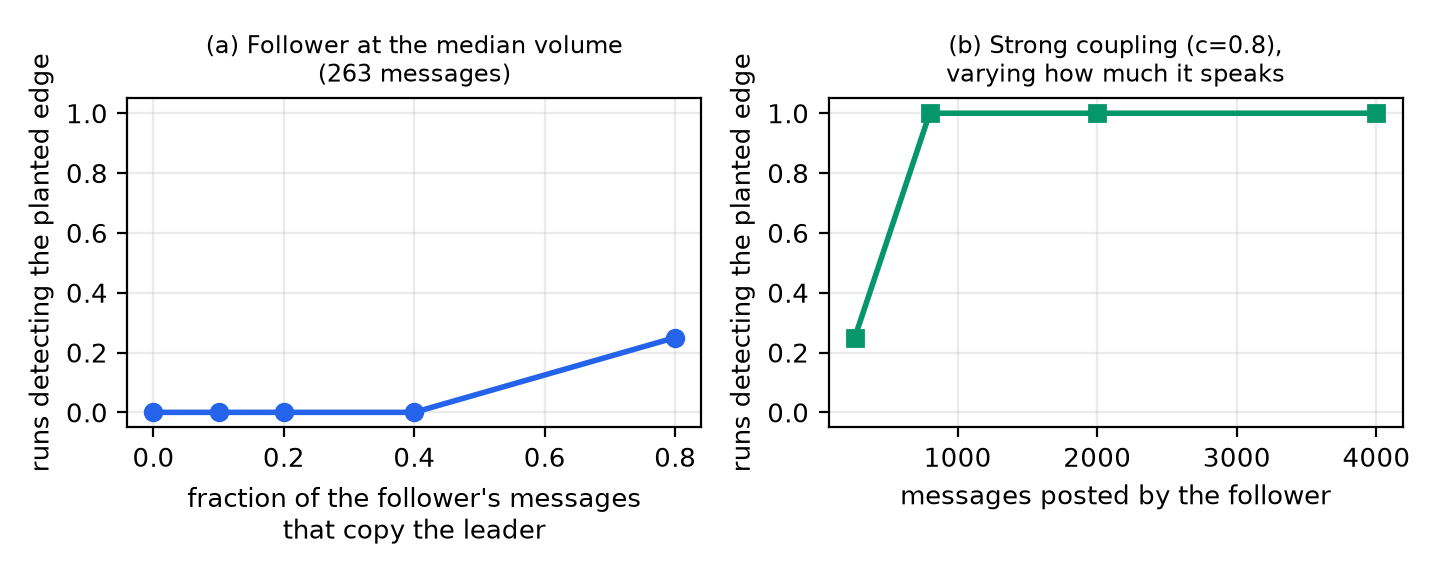
\includegraphics[width=0.92\textwidth]{f4_power.png}
\caption{Detection of a planted follower under the repaired surrogate. Left, varying the fraction of
its messages that copy the leader, at the median agent's volume. Right, varying how much it speaks,
at strong coupling.}
\end{figure}

\paragraph{Humans in the channel.} Main-village \#general is now effectively human-free, with 3 human
messages in the window, so the question has to be asked in open-chat, where 32\% of messages come
from 124 human visitors. Pairwise, with humans collapsed into one node, 19 edges are certified.
Conditioning removes almost all the agent-to-agent structure and little of the rest: \textbf{four
edges survive, of which three run from humans to agents, one is agent to agent, and none run from an
agent to a human.} The asymmetry is not an artifact of the confound. It should be read carefully all
the same: topical dependence from a person to an agent is also what ordinary responsiveness looks
like, so the measurement supports only that the dependence is dyad-specific and directional, not
that anyone is steering a swarm.

\section{Reproducibility, and one limitation of it}

Every number in this paper is recomputed from committed analysis output by a verifier that fails on a
mismatch, and that verifier covers the prose of this paper as well as the figures.

One limitation should be stated plainly. Re-running the counts in the earlier stationarity sweep with
the same seeds and configuration, only one of the eight cells reproduced exactly; the remaining
differences were one or two replicates per cell. Seven of the eight published rates still fell within
the recomputed Wilson intervals, and no conclusion changed. The exception is the zero-drift cell under
the permutation null, where the published 1 of 30 falls just below the recomputed interval of
$[0.035, 0.256]$ for 3 of 30, and no result here depends on that cell.

The generator, estimator and BLAS configuration were investigated and ruled out as the source. The
most likely explanation is a library-level difference, particularly in scikit-learn's $k$-means
implementation within the symboliser, whose output can vary between versions. Every sweep now records
the environment it ran under: Python 3.14.6, numpy 2.5.1, scipy 1.18.0 and scikit-learn 1.9.0,
including the BLAS build and the number of BLAS threads each worker used.

This does not make the previously published counts exactly reproducible. It provides a more clearly
specified environment in which subsequent results can be checked. For that reason I report rates
alongside their confidence intervals rather than exact replicate counts. The distinction between
reproducing a result within its uncertainty and reproducing every individual count matters, and only
the first is claimed.

\section{Conclusion}

Applied to real agent chat, the standard recipe for ``who drives whom'' needs repair before it says
anything. Clock windows cannot separate a message from its answer at the speed agents reply, and what
they certify is matched by a null with no access to meaning. The turn-ordered grid that fixes this
breaks the circular-shift surrogate: family-wise error 0.90 against a nominal 0.05, caused by the
speaker sequence itself. Restricted permutation surrogates repair most of that, but they are flat
under drift rather than calibrated, they are mutually indistinguishable at this precision, and one of
them needs twice the surrogate draws anyone would think to use. A valid surrogate fixes calibration
but not confounding. What survives is small: two dyad-specific edges that do not replicate, an
undetermined answer set by conditioning resolution, and influence running from people into agents and
never back. \textbf{An influence graph should not guide decisions until its error rate, its confound,
its detection floor and its symboliser's fidelity are reported.}

\section*{Limitations}

\begin{itemize}
\item \textbf{Immediate-predecessor only.} The turn-ordered lag-1 measure sees influence from the
message directly before a reply. Influence acting over several turns, or through a room's accumulated
context, is out of scope.
\item \textbf{Discrete approximation to an event process.} Agent chat is event-based in continuous
time. The turn-ordered discretisation with a permutation surrogate is a practical fix, and the
continuous-time comparison above shows what that choice gives up.
\item \textbf{The mechanism behind the real 0.90 is not established.} The generator separates
turn-taking from drift and points at drift, but the largest cell anywhere in the design is 0.365.
\item \textbf{Symbolisation quality cannot be measured on the real logs.} The central result survives
an independent symboliser, but the edge count does not: it moves with alphabet size and with which
messages the topic model is fit on. The floor remains the largest unquantified threat.
\item \textbf{No ground truth in the real logs.} The validity argument rests on planted controls and
on the meaning-free null, not on recovering a known answer.
\item \textbf{Conditioning removes real influence too.} The conditional estimate discards influence
that works by shifting what the channel is talking about, which in a group chat may be a large part
of genuine influence. It is a lower bound on dyadic influence.
\item \textbf{The human result is exploratory.} It rests on one village and one window and should be
read as a lead.
\end{itemize}

\section*{Broader impact and ethics}

This work audits influence detection on a population of AI agents, which is dual-use. Used
defensively it helps an overseer decide what an influence graph is worth, and the main result is
deflationary: it tells practitioners to trust these outputs less, which reduces rather than increases
the chance of acting on a bad attribution. The same tooling could be used to identify the most
influential agent in a swarm in order to target it, or to surveil participants in a channel. Three
properties limit the misuse. The subjects are AI models; the dataset is already public under research
terms and no re-identification is added; and the measure is weak and local, recovering
immediate-predecessor topical dependence rather than any model of how to steer an agent.

The dataset's research terms were followed: research use only, no training on the data, no
re-identification, citation of the source, and notification of the authors of resulting publications.
Human participants appear only as an aggregate node or as anonymised visitor labels, never by name or
handle, and no content attributable to an individual person is reported. Message text and metadata
were read, never model weights or private user data.

The use of a large language model in this work is disclosed in the first-page footnote, as TMLR
requires.

\bibliographystyle{tmlr}
\bibliography{refs}

\end{document}
"               de-anonymised arXiv preprint
%   pdflatex "\def\TMLRMODE{accepted}% TMLR submission. Built 10 November 2026 from:
%   paper/00_PROSE_v1.md   the author's written sections, 78 figures auto-verified
%   report/REPORT_V2.md    the sprint report, every number recomputed by report/verify_v2.py
%
% ANONYMITY. \usepackage{tmlr} with no option is the anonymous submission mode: the tmlr
% package hides the author block itself. Switching to [preprint] de-anonymises for arXiv AND
% turns on the \ifpreprint branches below, which are the only places a name, a repository URL
% or the benchmark's distinctive name appears. So one source produces both documents and the
% anonymous build cannot leak an identifier that the preprint build adds.
%
% Build:  latexmk -pdf main.tex
\documentclass[10pt]{article}

% The mode is chosen at build time so that one source produces every variant and they cannot
% drift apart:
%   latexmk -pdf main.tex                                        anonymous TMLR submission
%   pdflatex "\def\TMLRMODE{preprint}% TMLR submission. Built 10 November 2026 from:
%   paper/00_PROSE_v1.md   the author's written sections, 78 figures auto-verified
%   report/REPORT_V2.md    the sprint report, every number recomputed by report/verify_v2.py
%
% ANONYMITY. \usepackage{tmlr} with no option is the anonymous submission mode: the tmlr
% package hides the author block itself. Switching to [preprint] de-anonymises for arXiv AND
% turns on the \ifpreprint branches below, which are the only places a name, a repository URL
% or the benchmark's distinctive name appears. So one source produces both documents and the
% anonymous build cannot leak an identifier that the preprint build adds.
%
% Build:  latexmk -pdf main.tex
\documentclass[10pt]{article}

% The mode is chosen at build time so that one source produces every variant and they cannot
% drift apart:
%   latexmk -pdf main.tex                                        anonymous TMLR submission
%   pdflatex "\def\TMLRMODE{preprint}\input{main}"               de-anonymised arXiv preprint
%   pdflatex "\def\TMLRMODE{accepted}\input{main}"               camera-ready
% Use build.py, which runs all of them and checks the anonymous output for leaks.
\providecommand{\TMLRMODE}{submission}
\makeatletter
\def\@tmlrpreprint{preprint}
\def\@tmlraccepted{accepted}
\ifx\TMLRMODE\@tmlrpreprint
  \usepackage[preprint]{tmlr}
\else
  \ifx\TMLRMODE\@tmlraccepted
    \usepackage[accepted]{tmlr}
  \else
    \usepackage{tmlr}
  \fi
\fi
\makeatother

\usepackage{hyperref}
\usepackage{url}
\usepackage{booktabs}
\usepackage{graphicx}
\usepackage{amsmath}

% Gate every identifying string on whether identity may be revealed at all. The flag to test is
% \if@accepted, NOT \if@preprint: tmlr.sty's [preprint] option sets BOTH, so \if@accepted is true
% for the preprint and the camera-ready and false only for the anonymous submission, which is
% exactly the condition wanted. Gating on \if@preprint alone also hid the repository URLs from the
% camera-ready, which is where this paper promises to give them. \if@accepted is internal to
% tmlr.sty, hence the \makeatletter. The anonymous build takes the second argument.
\makeatletter
\newcommand{\ifdeanon}[2]{\if@accepted#1\else#2\fi}
\makeatother
\newcommand{\benchname}{\ifdeanon{SwarmInfluence-Bench}{the benchmark}}

% An unmarked footnote, for the LLM-use disclosure. TMLR's FAQ requires the disclosure and names
% the location: authors must "mention explicitly in their submission that they have used this
% tool", "as a footnote on the first page". Verified against jmlr.org/tmlr/faq.html on 10 Nov 2026.
% It is therefore not optional, and it does not belong in Broader Impact, where it sat until now.
% Nothing in the policy asks for the vendor's name, so none is given.
\newcommand{\disclosurefootnote}[1]{%
  \begingroup\renewcommand\thefootnote{}\footnote{#1}\addtocounter{footnote}{-1}\endgroup}

\title{An Influence Graph Over AI Agents Certifies an Agent That Copies Nobody}

% Hidden by the tmlr package unless [accepted] or [preprint] is given.
\author{\name Manu Nicholas Jacob \email manunicholasjacob@gmail.com \\
        \addr Independent Researcher}

\def\month{11}
\def\year{2026}
\def\openreview{\url{https://openreview.net/forum?id=XXXXXXXXXX}}

\begin{document}
\maketitle

\begin{abstract}
Circular-shift surrogates can produce severely inflated false-positive rates when applied to
turn-ordered multi-agent conversations, reaching a family-wise error rate of 0.90 against a nominal
0.05. A generated benchmark separates two candidate mechanisms and points at non-stationary speaker
activity rather than turn-taking, which suppresses the failure rather than causing it. No setting of
either knob reproduces the observed 0.90, however, so what drives the full real-data failure remains
open. Restricted permutation surrogates substantially reduce the problem. Their error rate is flat
with respect to drift rather than at the nominal level, and for the global within-speaker variant it
depends on how many surrogate draws the null is built from. Calibration alone does not address
confounding, which motivates a conditional estimator validated against a benchmark with planted
ground truth. I also identify a symbolisation-dependent detection limit and develop label-free
diagnostics for it, and show that their calibration does not transport across degradation
mechanisms. The benchmark is released.
\end{abstract}

\disclosurefootnote{\textbf{Use of a large language model.} A large language model was used as an
assistive tool: to help write and run the analysis code, and to help draft this paper. The author is
responsible for every claim, number and figure. All results come from the released code run on the
public dataset, no result or reference is fabricated, and every number in this paper is recomputed
from committed analysis output by a verifier that fails the build on a mismatch.}

\section{Introduction}

When AI agents interact in a shared channel, it is useful to understand how they influence one
another. Information-theoretic methods offer a way to measure this through lagged transfer entropy,
surrogate testing, and per-agent influence scores. They are attractive because they require no
labels and no access to model internals, only a record of who said what and when. The reliability of
those measurements is what this paper examines.

Almost every demonstration of these detectors runs on synthetic traces with a planted leader, where
the analyst controls timing and vocabulary. Real agent chat is asynchronous, bursty, and written in
open language. The narrower question here is whether the standard recipe, applied to real agent
logs, returns anything an overseer should act on.

The audit runs on the AI Village corpus \citep{aidigest2026}, in which frontier models share chat
channels over eighteen months across four villages differing in size, lifetime and tempo, applying
the checks a reader should demand: planted controls, a meaning-free symboliser, replication in a
held-out window, and sensitivity to every parameter that had to be chosen.

\begin{enumerate}
\item The conventional circular-shift surrogate is \textbf{invalid} on turn-ordered agent chat: a
family-wise error rate of 0.90 against a nominal 0.05, caused by the structure of the speaker
sequence itself.
\item Restricted permutation surrogates restore most of the calibration, and re-certifying under one
\textbf{scrambles rather than shrinks} the answer: one channel loses all 11 of its edges, another
gains 15.
\item The three restricted variants are \textbf{mutually indistinguishable} at the precision reached
here, so the choice between them cannot be justified on error rate. The global within-speaker
variant additionally needs on the order of 200 surrogate draws, and over-fires by roughly a factor
of two at 100.
\item Calibration is not confounding, so a conditional estimate is added and validated on a released
benchmark with a known influence graph: common-cause false edges fall from 22.3 to 0.33, and on the
planted-edge instances precision rises from 0.17 to 0.80 with no loss of recall or power.
\item The same benchmark exposes a \textbf{symbolisation floor}. Below roughly 0.44 adjusted Rand
index between symboliser and truth, detection collapses whatever the estimator. Label-free
diagnostics detect that floor, but their calibration does not transport across degradation
mechanisms, and I report where it fails.
\item On the real channels two edges stand at every conditioning resolution, 18 are
\textbf{undetermined} between 0 and 13, none replicates out of sample, and what survives alongside
humans runs from people to agents.
\end{enumerate}

\section{Related work}

\paragraph{Transfer entropy and surrogates.} Transfer entropy \citep{schreiber2000} measures how much
a source's past reduces uncertainty about a target's next symbol beyond the target's own past.
Plug-in estimators are biased upward on short series, so significance rests on surrogate data, with
family-wise error controlled by a max-T test \citep{westfall1993}. The usual surrogate is a circular
time shift of the source.

\paragraph{Event-based data breaks the shift surrogate.} \citet{shorten2021}, on neural spike trains,
show that the conventional source-time-shift surrogate fails to represent the null hypothesis of
conditional independence for event-based processes, and adapt to that setting the nearest-neighbour
local permutation scheme of \citet{runge2018}. Agent chat is event-based in that sense: messages are
events in continuous time, not samples of a clocked signal. The correction is not a contribution of
this paper. The contribution is showing that the same failure carries over to multi-agent safety
monitoring, and that it can be severe enough to create apparent leaders where none exist.

\paragraph{The same failure, concurrently, in multi-agent reinforcement learning.}
\citet{papadopoulos2026} report a closely related surrogate failure in multi-agent
reinforcement-learning action series. Their agent pairs have zero influence by construction, yet
circular time shifts produce false-positive rates of 100\% and 98.2\% against a nominal 0.05. A
plain permutation surrogate fares no better in their setting, at 100.00\% and 99.95\%. Their
proposed correction restricts permutations to blocks of training time, which returns the rates to
5.25\% and 5.50\%.

There are important differences between their setting and this one. Their data consist of binary
actions recorded over twelve thousand training rounds, whereas these data are symbolised
natural-language messages arranged on a turn-ordered conversational grid. Their non-stationarity
comes from monotone drift associated with annealing exploration; here the relevant non-stationarity
appears in the speaker sequence. Neither result should be taken as a direct extension of the other.

Nevertheless, the fact that both approaches rely on restricted permutations is worth noting. Their
permutation blocks are defined by training time, while mine are defined by an agent's own speaking
positions. This provides convergent evidence that unrestricted temporal rearrangement can be
problematic in non-stationary multi-agent data. Their findings also serve as a useful warning for
the approach taken here, and the warning has a measured form rather than a rhetorical one: in their
data the unrestricted permutation failed as completely as the time shift, at 100.00\% against a
nominal 0.05. Permutation-based surrogates are not automatically protected against
non-stationarity, and what protects the one used here is the restriction, not the permutation. I
claim no priority over their result and view the two studies as complementary, addressing different
forms of structured multi-agent data.

\paragraph{Oversight under a budget.} AI-control research frames monitoring as resource constrained,
with a cost for false positives \citep{greenblatt2024}. An influence graph is one such measurement,
and its error rate is the concern here.

\paragraph{Clustering stability.} The idea of using clustering stability as a label-free quality
indicator is not new. It has a substantial history, including \citet{benhur2002},
\citet{lange2004}, von Luxburg's review of clustering stability \citep{vonluxburg2010}, and
\citet{tibshirani2005} on prediction strength. What is different in Section~\ref{sec:floor} is the
calibration of these diagnostics against a detection-performance floor rather than against cluster
recovery alone.

\section{Data and representation}

The AI Village dataset ships one gzipped-JSONL table per village. Four villages are used, differing
enough to test whether any finding is a property of one channel.

\begin{table}[h]
\centering
\begin{tabular}{lrrrrl}
\toprule
village & agent messages & agents & lifetime & human messages & busiest room \\
\midrule
main      & 205,726 & 58  & 576 days & 10,029 & \#general (166,715, 81\%) \\
open-chat &  35,483 & 23  &  66 days & 12,264 & \#general (all) \\
swarm     &   3,848 & 133 &   1 day  &      5 & room a (3,846) \\
game-jam  &     838 & 6   &   3 days &     36 & per-team rooms \\
\bottomrule
\end{tabular}
\caption{The four villages. A 2026 scaffolding change scopes each agent to its current room's
context, so the busiest room of each village is a self-contained influence substrate and is analysed
alone.}
\end{table}

The primary window is the final fourteen days of main-village \#general, 17 to 31 October 2026,
holding 8,800 agent messages. Twenty-two models posted at least 50 messages each and the directed
test uses the 15 busiest, giving 7,958 message events. Two scaffolding facts are disclosed rather
than corrected: the automated nudger was off throughout, and the unused \#best and \#rest rooms were
soft-deleted mid-window, which does not touch \#general.

\subsection{From open language to symbols}

Transfer entropy needs discrete symbols, so each message is mapped to a small alphabet before
influence is estimated, and that mapping is kept separate from the estimator. A topic symboliser
(TF-IDF then $k$-means, $k=8$) gives a message its topic cluster id, so paraphrases of one idea share
a symbol. A hash symboliser, a stable hash of the normalised text into $k=8$ buckets, has no notion
of meaning and serves as a null: an edge appearing under both lives in timing alone.

\subsection{The lag problem, and why clock windows cannot solve it}

A lag-1 transfer entropy compares window $t-1$ with window $t$, so influence landing inside one
window is invisible to it. Agent chat makes this binding. Among the fifteen analysed agents the gap
between consecutive messages by different speakers has a median of 28.1 seconds (25th percentile
9.2, 75th 66.2, 95th 159.3), so turn-taking is a seconds-scale process while any clock window wide
enough to hold two speakers is minutes wide and swallows both a message and its answer.

Both horns are measurable. At 30 seconds only 1.2\% of agent-windows hold a message, while 32.0\% of
replies already land in the same window as what they answer, rising to 84.4\% at five minutes. At
every width tried, the meaning-free hash null certifies comparably many edges, and more at five
minutes: 9 against 12 at thirty seconds, 17 against 19 at one minute, 27 against 44 at fifteen, and
19 against 17 at five. Whatever clock-window transfer entropy was detecting there, it was not shared
meaning.

\begin{figure}[h]
\centering
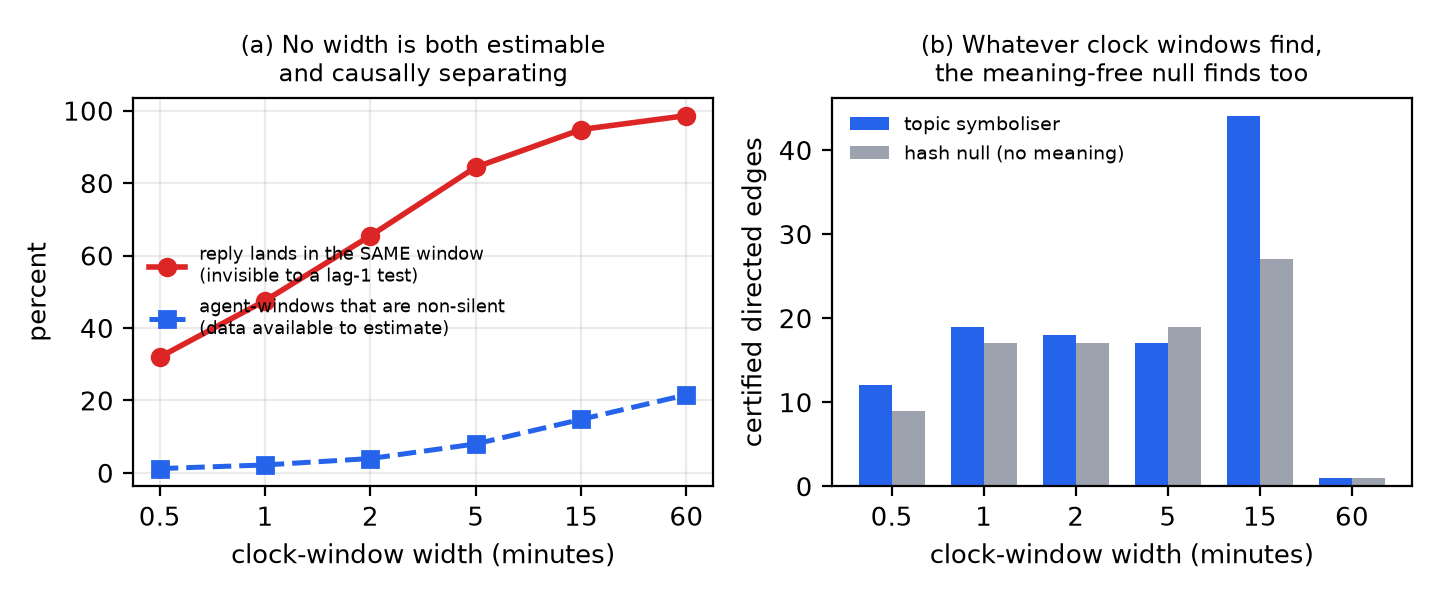
\includegraphics[width=0.92\textwidth]{f1_clock.png}
\caption{Clock-window transfer entropy on the 15 analysed agents of main-village \#general. Left,
the two failure modes as a function of window width. Right, edges certified under the topic
symboliser against the meaning-free hash null.}
\end{figure}

The bind is avoided by ordering messages canonically and letting one message be one tick. Each
agent's series carries its symbol where it spoke and a silent symbol elsewhere, so the lag-1
comparison is between a message and the one immediately before it. The cost is that the measure
captures immediate-predecessor influence only.

\section{The surrogate failure, and two explanations that did not hold}
\label{sec:failure}

An agent is planted into the real stream, drawing its symbols from the channel's marginal and
coupled to nothing at all. It is certified as driving something in 3 of 8 runs when it posts 50
messages, and in 8 of 8 at 100, 263, 600 and 1500 messages, with the mean largest $z$ rising from 5.6
to 12.3, 21.7, 38.3 and 71.7. The error grows with how much the agent speaks, which rules out a
small-sample explanation.

A planted agent could be dismissed as artificial, so the error rate is also measured directly.
Keeping the real speaker sequence and permuting the symbols globally leaves data with no directed
topical influence by construction. The shift surrogate certifies at least one edge in 9 of 10 such
replicates, a family-wise error rate of 0.90 against a nominal 0.05.

\paragraph{What breaks it is the speaker sequence.} Destroying one structure at a time isolates the
cause. Keeping the real speaker order and shuffling only symbols, the shift surrogate fires in 10 of
10 replicates; randomising the speaker order as well drops it to 0 of 10; uniform symbols with the
real order still give 6 of 10. So the driver is the structure of the speaker sequence, not the
symbol distribution and not sparsity. That sequence is far from random in two ways at once: it
repeats a speaker 36\% of the time and returns after one message 38\% of the time, and each agent's
activity is strongly non-stationary, with a median block-share coefficient of variation of 0.79.
Shuffling the order destroys both at once, so this ablation cannot say which of the two mattered.

\subsection{Two explanations I proposed, and the benchmark refuted both}

I initially attributed the failure to mutual exclusivity: only one agent can speak at each tick, so
shifting individual timelines could create overlaps that never occurred in the original
conversation. The benchmark did not support this explanation. A generated channel with exactly one
speaker per tick and steady activity produced an error rate of just 0.025, 95\% Wilson
$[0.011, 0.057]$, far below the 0.90 observed in the real data. Mutual exclusivity alone therefore
cannot explain the failure.

I then suspected turn-taking. In the real channel, speakers repeat 36\% of the time and return after
exactly one message 38\% of the time. However, adding a Markov speaker chain to the generator
produced the opposite result. Turn-taking suppressed the error rather than increasing it. At the
nominal knob values and with no drift the surrogate certified nothing at all across 200 replicates,
while removing turn-taking and introducing drift raised the rate to 0.365. The contribution from
drift was $+0.340$, compared with $-0.025$ for turn-taking. The same inversion appears in the arm
calibrated so that the generated channel reproduces the real channel's measured repeat, return and
block-share statistics rather than merely carrying those numbers as settings: there, turn-taking
alone also certifies nothing, and drift alone gives 0.065.

Neither mechanism, nor their combination in the tested design, reproduced the real-data error rate of
0.90. The largest cell anywhere in the design is 0.365. The real-data ablation removes turn-taking
and non-stationarity together, while the generator separates them. The results point to
non-stationary activity, but the remaining gap means the mechanism behind the full real-data failure
is not yet established.

Every figure above comes from the run at 200 surrogate draws. The first version of this analysis
used 100, which inflates both nulls on the same 2,400 instances: the circular shift fires 53 times
where the 200-draw run does not, against 18 the other way (exact McNemar $p = 3.9 \times 10^{-5}$),
and the permutation surrogate 83 against 20 ($p = 2.7 \times 10^{-10}$). Every qualitative conclusion
in this section is the same at both settings, which is why they are worth stating at all. The
numbers are not, so the draw count belongs in the caption.

\section{The repair, compared}
\label{sec:repair}

Following the local-permutation idea of \citet{runge2018} as adapted by \citet{shorten2021}, each
source keeps its speaking positions and only its symbols are permuted among them. Speaking pattern,
sparsity and turn-taking are preserved exactly, and only the correspondence between symbol and time
is destroyed. On the same destroyed-structure real data the family-wise error rate falls to 0.063
over 300 replicates, 95\% Wilson $[0.041, 0.097]$. The planted uncoupled agent is never certified: 0
of 5 at both 263 and 1500 messages, with mean max $z$ of 2.8 in each case against 22.0 and 68.3
under the shift surrogate.

\begin{figure}[h]
\centering
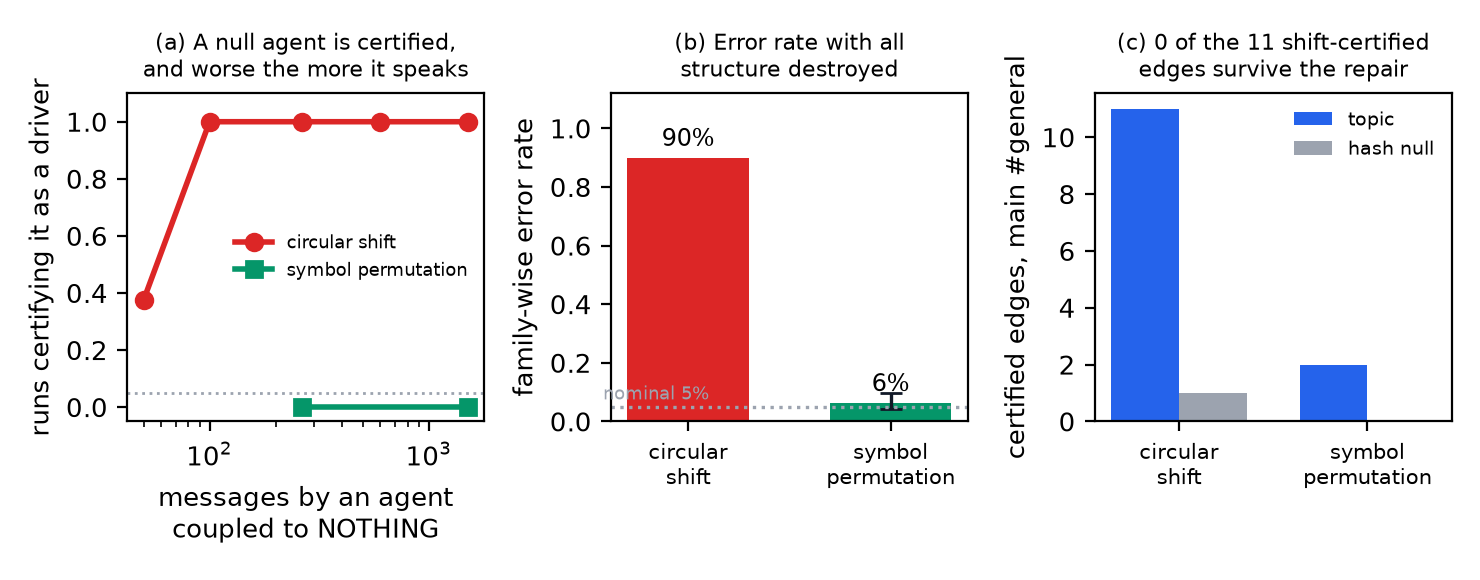
\includegraphics[width=\textwidth]{f2_null.png}
\caption{Left, how often an agent coupled to nothing is certified as a driver, under each surrogate.
Middle, family-wise error rate measured on data with all structure destroyed, with a Wilson
interval; the dotted line is the nominal 0.05. Right, what each surrogate certifies on the real
channel.}
\end{figure}

\subsection{How many surrogate draws are needed}

The number of surrogate draws matters more than I initially appreciated. In a paired comparison of
300 instances, where all four surrogates run on identical symbol grids so the outcomes are paired,
the global permutation surrogate produced a false-positive rate of 0.1167 with 100 draws, falling to
0.0700 with 200 draws, 95\% Wilson $[0.046, 0.105]$. This difference is statistically significant
(exact McNemar $p = 0.0043$). The block-local and Runge local permutations were less sensitive to the
increase: their corresponding rates changed from 0.0900 to 0.0767 and from 0.0967 to 0.0800.

At 200 draws, the global permutation's interval covers the nominal 0.05 and overlaps the real-data
estimate of 0.0633 $[0.0409, 0.0968]$. The real-data result is therefore corroborated rather than
overstated. For practical use, the important point is that reducing the number of surrogate draws
can materially change the result. In particular, the global permutation over-fires at 100 draws by
approximately a factor of two. I would therefore not treat the choice of draw count as a minor
computational detail.

The same correction applies to the benchmark-wide estimate. That figure was 0.0942 at 100 draws.
Repeating all 2,400 instances at 200 draws gives \textbf{0.0679}, 95\% Wilson $[0.0585, 0.0787]$,
and the paired difference is large: 83 instances fire at 100 draws and not at 200, against 20 the
other way, $p = 2.7 \times 10^{-10}$. The conclusion it supports is unchanged, because the interval
still excludes the nominal 0.05. So the permutation repair does carry a residual inflation on clean
generated data, but it is about a third above nominal rather than nearly double.

One limit on this recommendation. I compared 100 draws against 200 and did not test any larger
value, so what the experiment establishes is that 100 is too few, not that 200 is enough. Two
hundred is a lower bound on the draw count rather than a converged setting, and a practitioner whose
conclusions sit near a decision boundary should check their own sensitivity rather than adopt the
number.

\subsection{Choosing a repair, when the error rate cannot choose}

The comparison of the three permutation-based repairs does not produce a clear winner. All four
surrogates were evaluated on identical symbol grids across 300 pure-null replicates, so the
comparison reflects differences between the null models rather than differences between datasets.

\begin{table}[h]
\centering
\begin{tabular}{lrrrl}
\toprule
surrogate & FWER, 100 draws & FWER, 200 draws & 95\% Wilson at 200 & nominal 0.05 \\
\midrule
circular shift                   & 0.0433 & \textbf{0.0333} & $[0.018, 0.060]$ & inside \\
global within-speaker permutation & 0.1167 & \textbf{0.0700} & $[0.046, 0.105]$ & inside \\
block-local permutation          & 0.0900 & \textbf{0.0767} & $[0.052, 0.112]$ & excluded \\
local permutation \citep{runge2018} & 0.0967 & \textbf{0.0800} & $[0.054, 0.116]$ & excluded \\
\bottomrule
\end{tabular}
\caption{Four surrogates on identical symbol grids, 300 pure-null replicates, at both draw counts.}
\end{table}

At 200 draws, paired on the same 300 instances, the circular shift is not significantly different
from the global permutation ($p = 0.0614$), although it differs from block-local permutation
($p = 0.0294$) and from Runge's local permutation ($p = 0.0201$). At 100 draws it differed from all
three, which is the draw-count artifact again. The three repairs remain statistically
indistinguishable from one another, with pairwise $p$-values of 0.85, 0.65 and 1.00. The apparent
differences in their error rates are not sufficient to establish a ranking.

Choosing between them therefore requires more than calibration, and two readings pull against each
other. Runge's local permutation has the strongest methodological justification for preserving the
structure it is intended to preserve, and it follows the approach adapted to event data by
\citet{shorten2021}. Block-local permutation is more heuristic and introduces a free parameter that
has not been tuned. Global permutation is the simplest. On the other hand, the global permutation has
the most favourable interval relative to the nominal rate, and is the only repair that costs nothing
measurable against the shift on clean stationary data, although neither difference is statistically
established. I do not consider the observed error rates sufficient to select one repair over the
others. The choice should be guided by the structure the null is intended to preserve and the
assumptions that can be justified for the data.

\subsection{When to use the repair}

A drift sweep gives the practical reading. Across 150 replicates per cell at 200 surrogate draws,
the circular shift degrades steadily as activity drift increases while the three repairs do not.

\begin{table}[h]
\centering
\begin{tabular}{lrrrr}
\toprule
activity drift & circular shift & global permutation & block-local & local \\
\midrule
0.0 & \textbf{0.013} & 0.093 & 0.080 & 0.093 \\
0.3 & 0.100 & 0.100 & 0.093 & 0.120 \\
0.6 & \textbf{0.193} & 0.053 & 0.047 & 0.067 \\
0.9 & \textbf{0.380} & 0.087 & 0.080 & 0.080 \\
\bottomrule
\end{tabular}
\caption{Family-wise error on pure nulls as activity drift increases, 150 replicates per cell, 200
surrogate draws. Every certified edge is a false positive by construction.}
\end{table}

The pattern is supported by a formal trend test rather than by eye. A Cochran-Armitage test across
the four ordered drift levels gives the circular shift $z = 8.667$, $p < 10^{-15}$, and gives every
repair nothing: $p = 0.51$ for the global permutation, 0.63 for block-local and 0.37 for local. The
same pattern holds at both surrogate draw counts, so it does not depend on that choice.

The repairs are therefore flat under drift rather than calibrated. Only one of the four global
permutation intervals covers the nominal 0.05, and the rest sit nearer 0.09, so what the repair buys
is insensitivity to drift rather than correctness. One asymmetry should be stated rather than
hidden: block-local covers nominal in three of the four cells where the global repair covers one.
The two remain pairwise indistinguishable, so this is not grounds to switch the recommendation, but
it does mean the global repair cannot be described as the best-calibrated under drift.

The results also show why the repair should not be treated as universally preferable. At zero drift
the circular shift has an error rate of 0.013, while the three repairs are all around 0.08 to 0.09.
That advantage is gone by the first drift step: at drift 0.3 the shift reads 0.100 against the global
permutation's 0.100 and block-local's 0.093, so the crossover falls between drift 0.0 and 0.3 rather
than at some higher level. By drift 0.6 the shift is roughly four times the repairs. If a channel has
been checked and found stationary, the circular shift may be sufficient. When activity is
non-stationary the repairs are the more stable choice, and the margin for error on that judgement is
narrow, because the crossover arrives by the first drift level tested.

\section{Continuous time, and what the repair cannot test}

An earlier analysis identified continuous-time estimation as the principled option for event data
but did not evaluate it. Running the continuous-time estimator CoTETE on both channels certifies 0
edges in either case, compared with 2 for main-village and 18 for open-chat under the discrete,
turn-ordered analysis. Its highest $z$-scores are 3.062 and 3.980, below the respective max-T
thresholds of 4.171 and 4.308.

At first these results might appear to contradict the symbol-based analysis. The two estimators
operate on different information, however. CoTETE's public API takes event times with no symbol
channel, while the transfer-entropy analysis here uses topic symbols. To test whether this
difference explains the results, I reduced the data to timing alone, replacing every spoken symbol
with the same code. Under this representation the estimator used here also detects 0 edges in both
channels, matching CoTETE. Using the circular-shift surrogate instead produces 12 and 3 edges. So
neither method detects relationships from event timing alone in these channels, and the edges found
by the symbol-based analysis depend on symbol correspondence, which the continuous-time estimator
cannot access.

Two caveats attach to those $z$-scores, and the second attaches to the larger of them. Point
estimates from this estimator are stochastic to about 17\% across repeated runs, so none of these
values should be read to more than two significant figures. And open-chat's highest $z$, the 3.980,
belongs to the one pair whose surrogate draws mostly failed: it needed 1,936 failed draws to obtain
100 successes, a 4.9\% success rate. Those surrogates are conditioned on being estimable, so that
pair's null is biased in an unknown direction. The conclusion does not rest on it, since that pair
falls below threshold and so does every other pair, but the number should not be quoted as a clean
measurement. The failures themselves were a defect rather than a property of the data: an enlarged
exclusion window can empty the neighbour search on sparse bursty event trains and raise an error
that terminates a whole pair, with no handling at the public entry point. This has been reported
upstream.

There is also a fundamental limitation in applying the recommended permutation surrogate to
timing-only data. When every event carries the same symbol, permuting those symbols changes nothing.
The observed statistic and the surrogate null are identical, making the test exactly degenerate:
standard deviation 0 across all 210 pairs and $p = 1.0$ everywhere. \textbf{The repair has zero power
against timing structure by construction.} The permutation surrogate is appropriate for testing
relationships in the symbol sequence, but it does not answer whether relationships exist in event
timing. These are different questions, and choosing one null means giving up the ability to test the
other with that procedure.

\section{Confounding, and what conditioning removes}

A valid surrogate fixes calibration but not confounding. If every agent tracks a drifting channel
topic, every pair is genuinely dependent through the channel, and pairwise transfer entropy cannot
tell that from direct influence. I therefore also report a \textbf{conditional} estimate, which asks
whether a source's last message adds anything about a target's next one beyond the target's own
history and the channel's recent state. The conditioning variable is the modal symbol of the last
twelve messages, excluding the immediately preceding one so that it does not simply restate the
source.

On a generated benchmark whose decisive instances contain no influence while every agent tracks a
shared drifting topic, so that any certified edge is common cause, pairwise transfer entropy
certifies \textbf{22.3} edges on average and conditioning takes that to \textbf{0.33}, lifting pooled
precision on the four-edge instances from 0.17 to \textbf{0.80} at a recall of 1.0 either way. Across
couplings from 0.05 to 0.8 the conditional test still finds the planted edge in 3 of 3 runs, so the
gain costs no power.

The benchmark flatters the conditional estimator, since its common cause is a shared modal topic and
the conditioning variable is the channel's modal topic. The real channels are harder, and
conditioning there costs degrees of freedom: a 9-symbol alphabet with a 9-valued context gives 6,561
cells against about 7,900 ticks, so that variable is also coarsened to 4 and 2 values.

\begin{table}[h]
\centering
\begin{tabular}{lrrrr}
\toprule
channel & pairwise & conditional, 9 values & 4 values & 2 values \\
\midrule
main \#general      & 2  & \textbf{2, the same two edges} & 2 & 3 \\
open-chat \#general & 18 & \textbf{0} & \textbf{7} & \textbf{13} \\
swarm, room a       & 1  & \textbf{0} & & \\
\bottomrule
\end{tabular}
\caption{Conditioning at three resolutions. Main-village's two edges are robust to that choice;
open-chat's zero is not.}
\end{table}

At the finest resolution the open-chat test is degenerate, its surrogate sitting above the observed
statistic for 65\% of pairs with the largest $z$ in the family only 4.4, so it is failing to reject
rather than finding nothing to reject. Open-chat's structure therefore remains
\textbf{undetermined}: depending on the conditioning resolution, between 0 and 13 of its 18 edges may
survive. That resolution is a free parameter an analyst would set once and never revisit. This is a
property of the channel rather than the estimator: on structure-free real data the conditional test
fires in 2 of 40 replicates, an error rate of 0.05 with a mean $z$ of $-0.001$, so it is nominal
rather than conservative.

\section{The symbolisation floor}
\label{sec:floor}

Everything these methods produce is downstream of turning text into symbols. On the benchmark, where
the underlying topics are known, detection performance drops sharply when agreement between the
symboliser and the ground truth falls below roughly ARI 0.44, and this behaviour appears across the
tested estimators. Importantly, the false-positive rate can look \emph{better} below this point,
because the shared topic structure needed to produce confounded detections is no longer represented
reliably. A pipeline that stops detecting relationships may therefore have lost the signal it needs
rather than become more reliable, and nothing downstream of the symboliser can tell those apart.

\subsection{Detecting the floor without labels}

That degradation can be detected without ground-truth labels. Across the nine-level benchmark sweep,
three statistics separate the below-floor cases with zero errors: seed stability at a threshold of
0.623, agreement with LSA at 0.646, and the Calinski-Harabasz index at 138.9. Seed stability here is
the \textbf{minimum} pairwise agreement across seeds, not the mean; the mean variant makes one error,
at a different threshold of 0.791. Silhouette has the strongest correlation with true ARI, at 0.979,
but is not useful for identifying the boundary because its threshold falls within a gap of just
0.002. A statistic that tracks clustering quality most closely is not necessarily the best one for
making a classification decision.

Error count cannot choose among the three that were perfect, so I tested whether each threshold still
means what it meant when the channel changes for reasons other than topic separability. Applying each
cut unchanged to thirty cells that vary turn-taking, drift, agent count, volume skew, message length
and corpus size, twenty-seven of which hold true ARI at exactly 1.000:

\begin{table}[h]
\centering
\begin{tabular}{lrrrr}
\toprule
diagnostic & cut & errors where fitted & errors, nuisance set & of those at true ARI 1.000 \\
\midrule
seed stability, min across seeds & 0.623 & 0 & 2 & \textbf{0} \\
LSA agreement                    & 0.646 & 0 & 2 & \textbf{0} \\
Calinski-Harabasz                & 138.9 & 0 & 6 & \textbf{3} \\
\bottomrule
\end{tabular}
\caption{Whether a cut fitted on the vocabulary-overlap mechanism survives a change in the channel
that is not a change in topic separability.}
\end{table}

The two bounded statistics err only on the short-message cells, where the symbolisation genuinely has
degraded. Calinski-Harabasz additionally condemns all three cells whose true ARI is exactly 1.000,
for no reason beyond the corpus holding 2,000 messages rather than 8,000, where it reads 76 to 77
against its own cut of 138.9. It is unbounded and grows with sample size, so a published numeric
threshold for it carries no meaning on another corpus. That is why I recommend the two bounded
statistics and not the index that matched them on error count. \textbf{A cut that moves with the
corpus is not a floor cut.}

This is not a weak statistic being discarded on a technicality. Calinski-Harabasz correlates with
true ARI at 0.973, almost as closely as silhouette, and unlike silhouette it classifies the floor
perfectly where it was fitted. It still cannot carry a published threshold. That is the sharper form
of the point above: neither the statistic that tracks quality most closely nor the one that
classifies best on the fitting mechanism is necessarily the one whose cut another researcher can
reuse.

There are important limits to this result. The effective sample size is nine rather than 54, because
the classification label is determined by overlap level. There are no observations between ARI 0.444
and 0.222, so the exact location of the boundary within that interval remains unknown. These
diagnostics classify whether a result is below the tested detection floor; they do not estimate ARI,
and their behaviour is flat between 0.68 and 1.00, and not even monotone there. The benchmark also
uses a single degradation mechanism with a known and correct value of $k$, whereas the true number of
topics in real conversations is unknown. I therefore treat 0.44 as a benchmark-specific, bracketed
result rather than a universal threshold.

\subsection{A contradiction the diagnostic lost}

I initially used these diagnostics to classify one real channel, open-chat, as below the
symbolisation floor. That conclusion did not agree with the channel's measured results: open-chat
certified 18 and 22 edges under the two symbolisers, compared with 2 and 1 for main-village, and its
hash-based null certified zero edges. Rather than treating this disagreement as evidence that the
original measurements were wrong, I revisited the diagnostic itself.

The problem was the choice of $k$. Repeating the comparison with the same channels, loader and window
reproduced the published $k=8$ results to the digit. At $k=4$, however, open-chat reached stability
scores of 0.950 and 0.978, the highest values produced by either channel across the tested settings,
and both exceeded the diagnostic thresholds. The earlier below-floor classification was therefore a
conclusion about one arbitrary choice of $k$, not a reliable statement about the channel. Message
length does not explain the difference either: 27.1\% of main-village messages contain fewer than
five tokens, compared with 2.3\% in open-chat, so the short-message channel is the one the diagnostic
cleared.

This correction changes how the symbolisation results should be read, and it withdrew three claims.

\begin{enumerate}
\item \textbf{The claim that no topic signal remains below the floor is too strong.} The
circular-shift surrogate recovers all four planted edges at every tested overlap level, including
0.95, where ARI is 0.011. The observed collapse is in the permutation null, not necessarily in the
underlying data.
\item \textbf{ARI 0.44 cannot be treated as a universal detection threshold.} When the shared-topic
parameter is 0, detection continues down to ARI 0.296, so the boundary depends on both the
symboliser and the channel.
\item \textbf{Edge counts cannot be used as a measure of symboliser quality.} Even at ARI exactly
1.000, changing the shared-topic parameter alone moves the permutation edge count from 5 to 78.
\end{enumerate}

The diagnostics also do not transfer reliably outside the mechanism on which they were evaluated.
Their balanced accuracy falls from 1.00 to 0.75 and 0.571 under a known mismatch in $k$. All seven
errors made by seed stability are false below-floor classifications, and in every one of those cases
the detector still identifies all planted edges; of the fourteen cells it condemned, eleven had full
conditional recall. The failure direction is the dangerous one: it condemns working symbolisations.

This was an important correction to my own interpretation. I introduced a diagnostic to check whether
the symbolisation was reliable, applied it to the real channels, and found that it contradicted
measurements already in hand. Investigating that contradiction showed the diagnostic was sensitive to
an arbitrary modelling choice. The result is not that the original measurements were wrong, but that
the control was being asked to support a broader conclusion than the evidence allowed. These
diagnostics remain useful within their tested setting, and \textbf{no channel-level floor verdict
should be issued from a single $k$}.

\section{The benchmark}

Real logs have no ground truth, so the common-cause question could not be settled on them. The
generator used here makes the influence graph known by construction: it decides, in code, who speaks
at which tick, on which topic, and who reacts to whom. Surface text is a separate, replaceable layer
drawn from disjoint per-topic vocabularies, so the whole thing runs offline and a detector still has
to symbolise raw text rather than read the labels. Turn-taking and activity drift are independent
knobs, so the two can be varied one at a time, and the generator reproduces its earlier behaviour
bit for bit when both are zero.

\benchname{} is released with 150 tests covering the generator, the detector harness, the text layer,
the floor analysis and the turn-taking factorial.
\ifdeanon{Code and benchmark:
\url{https://github.com/manunicholasjacob/swarm-influence-bench} and
\url{https://github.com/manunicholasjacob/swarm-influence-audit}.}{Code and benchmark are publicly
released; the links are withheld here for anonymity and will be given in the camera-ready version.}

One property of the benchmark must be stated when its numbers are quoted. Planting an edge displaces
other agents' speaking turns, so the generated instances contain real lag-1 dependencies that the
label set does not list. Precision measured against those labels is therefore a \textbf{lower bound}
for any detector, and what the benchmark supports is the comparison between two estimators rather
than the absolute value of either.

\section{What an overseer should do}

Six inexpensive controls should be included whenever an influence graph over an agent channel is
published.

\begin{enumerate}
\item \textbf{Plant an agent coupled to nothing, at your channel's volumes, and check it is not
certified.} This one test would have caught the failure reported here, at one run per volume.
\item \textbf{Measure the error rate directly}, by destroying the structure your method claims to
find and checking the family-wise rate is near nominal. If it is not, your surrogate does not match
your data.
\item \textbf{Preserve the speaker sequence in your surrogate.} Any surrogate that moves an agent's
messages in time will disturb it, and \citet{shorten2021} is the principled route. Use at least 200
surrogate draws, because at 100 the global within-speaker permutation over-fires by roughly a factor
of two.
\item \textbf{Establish the detection floor before interpreting an absence.} ``No edges'' and ``no
influence'' are different claims.
\item \textbf{Condition on the channel, report both numbers, and sweep the resolution.} Pairwise and
conditional bound the answer, and the gap between them is the result. Conditioning costs cells, so
check whether your answer is an artifact of how finely you conditioned. On one channel here it was.
\item \textbf{Report how well your symboliser agrees with the truth, on data where you know it.}
Everything is downstream of turning text into symbols, and below roughly ARI 0.44 detection
collapses whatever the estimator. I have found this control in no influence-detection paper, and it
is also the one that cannot be run on real logs, which is why the floor remains the largest
unquantified threat here.
\end{enumerate}

Two habits follow: publish a meaning-free null's count beside the real one, and require held-out
replication before calling a graph a structure.

\section{The real channels, and what survives}

Re-running every channel under the repaired surrogate changes the answers, and not in one direction.

\begin{table}[h]
\centering
\begin{tabular}{lrrr}
\toprule
channel & window messages & shift: topic / hash & permutation: topic / hash \\
\midrule
main \#general      & 8,800 & 11 / 1 & 2 / 0 \\
open-chat \#general & 8,226 & 3 / 0  & 18 / 0 \\
swarm, room a       & 3,846 & 2 / 1  & 1 / 0 \\
\bottomrule
\end{tabular}
\caption{The same channels under both surrogates, with the meaning-free hash null beside each.}
\end{table}

In main-village, \textbf{none} of the 11 edges the standard recipe certifies survives the repair, and
the two the valid surrogate certifies were not among them. In open-chat the correction runs the other
way, 3 edges becoming 18, because pathological pairs inflate the max-T threshold and raise the bar
for everything else. An invalid surrogate does not simply add false positives; it scrambles the
result.

Main-village's two edges are the strongest thing here and they are still not a finding, because they
do not replicate: the adjacent fourteen-day window certifies nothing at all under either estimator.
Given the detection floor, that silence is as consistent with the test sitting near its limit as with
the edges being absent, and the two cannot be separated. Power is governed by how much an agent says
as much as by how strongly it copies, and it is channel-specific: in main-village a planted follower
copying on 80\% of its messages is caught only 1 time in 4, while in open-chat one copying 10\% of
the time is caught 3 times in 4. Replication is weak everywhere: under the standard recipe the
adjacent window shares 1 edge out of 8 and 4, and that edge is also the only one the hash null
certifies. No certified edge in this work replicates out of sample.

\begin{figure}[h]
\centering
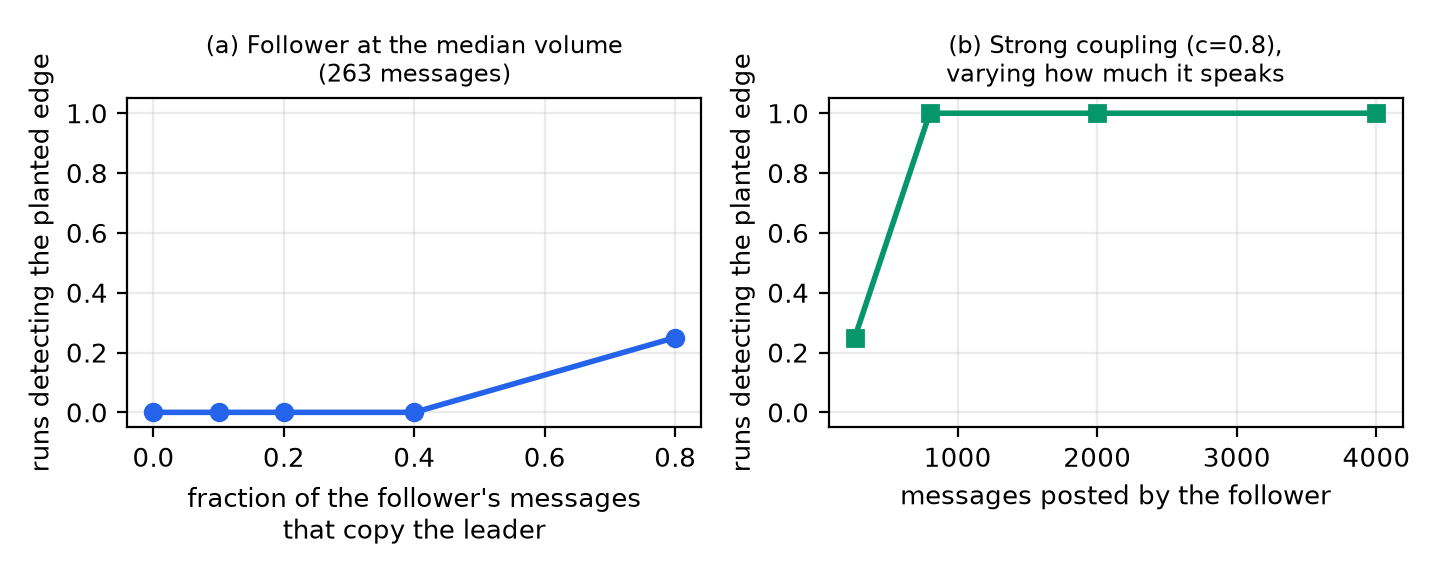
\includegraphics[width=0.92\textwidth]{f4_power.png}
\caption{Detection of a planted follower under the repaired surrogate. Left, varying the fraction of
its messages that copy the leader, at the median agent's volume. Right, varying how much it speaks,
at strong coupling.}
\end{figure}

\paragraph{Humans in the channel.} Main-village \#general is now effectively human-free, with 3 human
messages in the window, so the question has to be asked in open-chat, where 32\% of messages come
from 124 human visitors. Pairwise, with humans collapsed into one node, 19 edges are certified.
Conditioning removes almost all the agent-to-agent structure and little of the rest: \textbf{four
edges survive, of which three run from humans to agents, one is agent to agent, and none run from an
agent to a human.} The asymmetry is not an artifact of the confound. It should be read carefully all
the same: topical dependence from a person to an agent is also what ordinary responsiveness looks
like, so the measurement supports only that the dependence is dyad-specific and directional, not
that anyone is steering a swarm.

\section{Reproducibility, and one limitation of it}

Every number in this paper is recomputed from committed analysis output by a verifier that fails on a
mismatch, and that verifier covers the prose of this paper as well as the figures.

One limitation should be stated plainly. Re-running the counts in the earlier stationarity sweep with
the same seeds and configuration, only one of the eight cells reproduced exactly; the remaining
differences were one or two replicates per cell. Seven of the eight published rates still fell within
the recomputed Wilson intervals, and no conclusion changed. The exception is the zero-drift cell under
the permutation null, where the published 1 of 30 falls just below the recomputed interval of
$[0.035, 0.256]$ for 3 of 30, and no result here depends on that cell.

The generator, estimator and BLAS configuration were investigated and ruled out as the source. The
most likely explanation is a library-level difference, particularly in scikit-learn's $k$-means
implementation within the symboliser, whose output can vary between versions. Every sweep now records
the environment it ran under: Python 3.14.6, numpy 2.5.1, scipy 1.18.0 and scikit-learn 1.9.0,
including the BLAS build and the number of BLAS threads each worker used.

This does not make the previously published counts exactly reproducible. It provides a more clearly
specified environment in which subsequent results can be checked. For that reason I report rates
alongside their confidence intervals rather than exact replicate counts. The distinction between
reproducing a result within its uncertainty and reproducing every individual count matters, and only
the first is claimed.

\section{Conclusion}

Applied to real agent chat, the standard recipe for ``who drives whom'' needs repair before it says
anything. Clock windows cannot separate a message from its answer at the speed agents reply, and what
they certify is matched by a null with no access to meaning. The turn-ordered grid that fixes this
breaks the circular-shift surrogate: family-wise error 0.90 against a nominal 0.05, caused by the
speaker sequence itself. Restricted permutation surrogates repair most of that, but they are flat
under drift rather than calibrated, they are mutually indistinguishable at this precision, and one of
them needs twice the surrogate draws anyone would think to use. A valid surrogate fixes calibration
but not confounding. What survives is small: two dyad-specific edges that do not replicate, an
undetermined answer set by conditioning resolution, and influence running from people into agents and
never back. \textbf{An influence graph should not guide decisions until its error rate, its confound,
its detection floor and its symboliser's fidelity are reported.}

\section*{Limitations}

\begin{itemize}
\item \textbf{Immediate-predecessor only.} The turn-ordered lag-1 measure sees influence from the
message directly before a reply. Influence acting over several turns, or through a room's accumulated
context, is out of scope.
\item \textbf{Discrete approximation to an event process.} Agent chat is event-based in continuous
time. The turn-ordered discretisation with a permutation surrogate is a practical fix, and the
continuous-time comparison above shows what that choice gives up.
\item \textbf{The mechanism behind the real 0.90 is not established.} The generator separates
turn-taking from drift and points at drift, but the largest cell anywhere in the design is 0.365.
\item \textbf{Symbolisation quality cannot be measured on the real logs.} The central result survives
an independent symboliser, but the edge count does not: it moves with alphabet size and with which
messages the topic model is fit on. The floor remains the largest unquantified threat.
\item \textbf{No ground truth in the real logs.} The validity argument rests on planted controls and
on the meaning-free null, not on recovering a known answer.
\item \textbf{Conditioning removes real influence too.} The conditional estimate discards influence
that works by shifting what the channel is talking about, which in a group chat may be a large part
of genuine influence. It is a lower bound on dyadic influence.
\item \textbf{The human result is exploratory.} It rests on one village and one window and should be
read as a lead.
\end{itemize}

\section*{Broader impact and ethics}

This work audits influence detection on a population of AI agents, which is dual-use. Used
defensively it helps an overseer decide what an influence graph is worth, and the main result is
deflationary: it tells practitioners to trust these outputs less, which reduces rather than increases
the chance of acting on a bad attribution. The same tooling could be used to identify the most
influential agent in a swarm in order to target it, or to surveil participants in a channel. Three
properties limit the misuse. The subjects are AI models; the dataset is already public under research
terms and no re-identification is added; and the measure is weak and local, recovering
immediate-predecessor topical dependence rather than any model of how to steer an agent.

The dataset's research terms were followed: research use only, no training on the data, no
re-identification, citation of the source, and notification of the authors of resulting publications.
Human participants appear only as an aggregate node or as anonymised visitor labels, never by name or
handle, and no content attributable to an individual person is reported. Message text and metadata
were read, never model weights or private user data.

The use of a large language model in this work is disclosed in the first-page footnote, as TMLR
requires.

\bibliographystyle{tmlr}
\bibliography{refs}

\end{document}
"               de-anonymised arXiv preprint
%   pdflatex "\def\TMLRMODE{accepted}% TMLR submission. Built 10 November 2026 from:
%   paper/00_PROSE_v1.md   the author's written sections, 78 figures auto-verified
%   report/REPORT_V2.md    the sprint report, every number recomputed by report/verify_v2.py
%
% ANONYMITY. \usepackage{tmlr} with no option is the anonymous submission mode: the tmlr
% package hides the author block itself. Switching to [preprint] de-anonymises for arXiv AND
% turns on the \ifpreprint branches below, which are the only places a name, a repository URL
% or the benchmark's distinctive name appears. So one source produces both documents and the
% anonymous build cannot leak an identifier that the preprint build adds.
%
% Build:  latexmk -pdf main.tex
\documentclass[10pt]{article}

% The mode is chosen at build time so that one source produces every variant and they cannot
% drift apart:
%   latexmk -pdf main.tex                                        anonymous TMLR submission
%   pdflatex "\def\TMLRMODE{preprint}\input{main}"               de-anonymised arXiv preprint
%   pdflatex "\def\TMLRMODE{accepted}\input{main}"               camera-ready
% Use build.py, which runs all of them and checks the anonymous output for leaks.
\providecommand{\TMLRMODE}{submission}
\makeatletter
\def\@tmlrpreprint{preprint}
\def\@tmlraccepted{accepted}
\ifx\TMLRMODE\@tmlrpreprint
  \usepackage[preprint]{tmlr}
\else
  \ifx\TMLRMODE\@tmlraccepted
    \usepackage[accepted]{tmlr}
  \else
    \usepackage{tmlr}
  \fi
\fi
\makeatother

\usepackage{hyperref}
\usepackage{url}
\usepackage{booktabs}
\usepackage{graphicx}
\usepackage{amsmath}

% Gate every identifying string on whether identity may be revealed at all. The flag to test is
% \if@accepted, NOT \if@preprint: tmlr.sty's [preprint] option sets BOTH, so \if@accepted is true
% for the preprint and the camera-ready and false only for the anonymous submission, which is
% exactly the condition wanted. Gating on \if@preprint alone also hid the repository URLs from the
% camera-ready, which is where this paper promises to give them. \if@accepted is internal to
% tmlr.sty, hence the \makeatletter. The anonymous build takes the second argument.
\makeatletter
\newcommand{\ifdeanon}[2]{\if@accepted#1\else#2\fi}
\makeatother
\newcommand{\benchname}{\ifdeanon{SwarmInfluence-Bench}{the benchmark}}

% An unmarked footnote, for the LLM-use disclosure. TMLR's FAQ requires the disclosure and names
% the location: authors must "mention explicitly in their submission that they have used this
% tool", "as a footnote on the first page". Verified against jmlr.org/tmlr/faq.html on 10 Nov 2026.
% It is therefore not optional, and it does not belong in Broader Impact, where it sat until now.
% Nothing in the policy asks for the vendor's name, so none is given.
\newcommand{\disclosurefootnote}[1]{%
  \begingroup\renewcommand\thefootnote{}\footnote{#1}\addtocounter{footnote}{-1}\endgroup}

\title{An Influence Graph Over AI Agents Certifies an Agent That Copies Nobody}

% Hidden by the tmlr package unless [accepted] or [preprint] is given.
\author{\name Manu Nicholas Jacob \email manunicholasjacob@gmail.com \\
        \addr Independent Researcher}

\def\month{11}
\def\year{2026}
\def\openreview{\url{https://openreview.net/forum?id=XXXXXXXXXX}}

\begin{document}
\maketitle

\begin{abstract}
Circular-shift surrogates can produce severely inflated false-positive rates when applied to
turn-ordered multi-agent conversations, reaching a family-wise error rate of 0.90 against a nominal
0.05. A generated benchmark separates two candidate mechanisms and points at non-stationary speaker
activity rather than turn-taking, which suppresses the failure rather than causing it. No setting of
either knob reproduces the observed 0.90, however, so what drives the full real-data failure remains
open. Restricted permutation surrogates substantially reduce the problem. Their error rate is flat
with respect to drift rather than at the nominal level, and for the global within-speaker variant it
depends on how many surrogate draws the null is built from. Calibration alone does not address
confounding, which motivates a conditional estimator validated against a benchmark with planted
ground truth. I also identify a symbolisation-dependent detection limit and develop label-free
diagnostics for it, and show that their calibration does not transport across degradation
mechanisms. The benchmark is released.
\end{abstract}

\disclosurefootnote{\textbf{Use of a large language model.} A large language model was used as an
assistive tool: to help write and run the analysis code, and to help draft this paper. The author is
responsible for every claim, number and figure. All results come from the released code run on the
public dataset, no result or reference is fabricated, and every number in this paper is recomputed
from committed analysis output by a verifier that fails the build on a mismatch.}

\section{Introduction}

When AI agents interact in a shared channel, it is useful to understand how they influence one
another. Information-theoretic methods offer a way to measure this through lagged transfer entropy,
surrogate testing, and per-agent influence scores. They are attractive because they require no
labels and no access to model internals, only a record of who said what and when. The reliability of
those measurements is what this paper examines.

Almost every demonstration of these detectors runs on synthetic traces with a planted leader, where
the analyst controls timing and vocabulary. Real agent chat is asynchronous, bursty, and written in
open language. The narrower question here is whether the standard recipe, applied to real agent
logs, returns anything an overseer should act on.

The audit runs on the AI Village corpus \citep{aidigest2026}, in which frontier models share chat
channels over eighteen months across four villages differing in size, lifetime and tempo, applying
the checks a reader should demand: planted controls, a meaning-free symboliser, replication in a
held-out window, and sensitivity to every parameter that had to be chosen.

\begin{enumerate}
\item The conventional circular-shift surrogate is \textbf{invalid} on turn-ordered agent chat: a
family-wise error rate of 0.90 against a nominal 0.05, caused by the structure of the speaker
sequence itself.
\item Restricted permutation surrogates restore most of the calibration, and re-certifying under one
\textbf{scrambles rather than shrinks} the answer: one channel loses all 11 of its edges, another
gains 15.
\item The three restricted variants are \textbf{mutually indistinguishable} at the precision reached
here, so the choice between them cannot be justified on error rate. The global within-speaker
variant additionally needs on the order of 200 surrogate draws, and over-fires by roughly a factor
of two at 100.
\item Calibration is not confounding, so a conditional estimate is added and validated on a released
benchmark with a known influence graph: common-cause false edges fall from 22.3 to 0.33, and on the
planted-edge instances precision rises from 0.17 to 0.80 with no loss of recall or power.
\item The same benchmark exposes a \textbf{symbolisation floor}. Below roughly 0.44 adjusted Rand
index between symboliser and truth, detection collapses whatever the estimator. Label-free
diagnostics detect that floor, but their calibration does not transport across degradation
mechanisms, and I report where it fails.
\item On the real channels two edges stand at every conditioning resolution, 18 are
\textbf{undetermined} between 0 and 13, none replicates out of sample, and what survives alongside
humans runs from people to agents.
\end{enumerate}

\section{Related work}

\paragraph{Transfer entropy and surrogates.} Transfer entropy \citep{schreiber2000} measures how much
a source's past reduces uncertainty about a target's next symbol beyond the target's own past.
Plug-in estimators are biased upward on short series, so significance rests on surrogate data, with
family-wise error controlled by a max-T test \citep{westfall1993}. The usual surrogate is a circular
time shift of the source.

\paragraph{Event-based data breaks the shift surrogate.} \citet{shorten2021}, on neural spike trains,
show that the conventional source-time-shift surrogate fails to represent the null hypothesis of
conditional independence for event-based processes, and adapt to that setting the nearest-neighbour
local permutation scheme of \citet{runge2018}. Agent chat is event-based in that sense: messages are
events in continuous time, not samples of a clocked signal. The correction is not a contribution of
this paper. The contribution is showing that the same failure carries over to multi-agent safety
monitoring, and that it can be severe enough to create apparent leaders where none exist.

\paragraph{The same failure, concurrently, in multi-agent reinforcement learning.}
\citet{papadopoulos2026} report a closely related surrogate failure in multi-agent
reinforcement-learning action series. Their agent pairs have zero influence by construction, yet
circular time shifts produce false-positive rates of 100\% and 98.2\% against a nominal 0.05. A
plain permutation surrogate fares no better in their setting, at 100.00\% and 99.95\%. Their
proposed correction restricts permutations to blocks of training time, which returns the rates to
5.25\% and 5.50\%.

There are important differences between their setting and this one. Their data consist of binary
actions recorded over twelve thousand training rounds, whereas these data are symbolised
natural-language messages arranged on a turn-ordered conversational grid. Their non-stationarity
comes from monotone drift associated with annealing exploration; here the relevant non-stationarity
appears in the speaker sequence. Neither result should be taken as a direct extension of the other.

Nevertheless, the fact that both approaches rely on restricted permutations is worth noting. Their
permutation blocks are defined by training time, while mine are defined by an agent's own speaking
positions. This provides convergent evidence that unrestricted temporal rearrangement can be
problematic in non-stationary multi-agent data. Their findings also serve as a useful warning for
the approach taken here, and the warning has a measured form rather than a rhetorical one: in their
data the unrestricted permutation failed as completely as the time shift, at 100.00\% against a
nominal 0.05. Permutation-based surrogates are not automatically protected against
non-stationarity, and what protects the one used here is the restriction, not the permutation. I
claim no priority over their result and view the two studies as complementary, addressing different
forms of structured multi-agent data.

\paragraph{Oversight under a budget.} AI-control research frames monitoring as resource constrained,
with a cost for false positives \citep{greenblatt2024}. An influence graph is one such measurement,
and its error rate is the concern here.

\paragraph{Clustering stability.} The idea of using clustering stability as a label-free quality
indicator is not new. It has a substantial history, including \citet{benhur2002},
\citet{lange2004}, von Luxburg's review of clustering stability \citep{vonluxburg2010}, and
\citet{tibshirani2005} on prediction strength. What is different in Section~\ref{sec:floor} is the
calibration of these diagnostics against a detection-performance floor rather than against cluster
recovery alone.

\section{Data and representation}

The AI Village dataset ships one gzipped-JSONL table per village. Four villages are used, differing
enough to test whether any finding is a property of one channel.

\begin{table}[h]
\centering
\begin{tabular}{lrrrrl}
\toprule
village & agent messages & agents & lifetime & human messages & busiest room \\
\midrule
main      & 205,726 & 58  & 576 days & 10,029 & \#general (166,715, 81\%) \\
open-chat &  35,483 & 23  &  66 days & 12,264 & \#general (all) \\
swarm     &   3,848 & 133 &   1 day  &      5 & room a (3,846) \\
game-jam  &     838 & 6   &   3 days &     36 & per-team rooms \\
\bottomrule
\end{tabular}
\caption{The four villages. A 2026 scaffolding change scopes each agent to its current room's
context, so the busiest room of each village is a self-contained influence substrate and is analysed
alone.}
\end{table}

The primary window is the final fourteen days of main-village \#general, 17 to 31 October 2026,
holding 8,800 agent messages. Twenty-two models posted at least 50 messages each and the directed
test uses the 15 busiest, giving 7,958 message events. Two scaffolding facts are disclosed rather
than corrected: the automated nudger was off throughout, and the unused \#best and \#rest rooms were
soft-deleted mid-window, which does not touch \#general.

\subsection{From open language to symbols}

Transfer entropy needs discrete symbols, so each message is mapped to a small alphabet before
influence is estimated, and that mapping is kept separate from the estimator. A topic symboliser
(TF-IDF then $k$-means, $k=8$) gives a message its topic cluster id, so paraphrases of one idea share
a symbol. A hash symboliser, a stable hash of the normalised text into $k=8$ buckets, has no notion
of meaning and serves as a null: an edge appearing under both lives in timing alone.

\subsection{The lag problem, and why clock windows cannot solve it}

A lag-1 transfer entropy compares window $t-1$ with window $t$, so influence landing inside one
window is invisible to it. Agent chat makes this binding. Among the fifteen analysed agents the gap
between consecutive messages by different speakers has a median of 28.1 seconds (25th percentile
9.2, 75th 66.2, 95th 159.3), so turn-taking is a seconds-scale process while any clock window wide
enough to hold two speakers is minutes wide and swallows both a message and its answer.

Both horns are measurable. At 30 seconds only 1.2\% of agent-windows hold a message, while 32.0\% of
replies already land in the same window as what they answer, rising to 84.4\% at five minutes. At
every width tried, the meaning-free hash null certifies comparably many edges, and more at five
minutes: 9 against 12 at thirty seconds, 17 against 19 at one minute, 27 against 44 at fifteen, and
19 against 17 at five. Whatever clock-window transfer entropy was detecting there, it was not shared
meaning.

\begin{figure}[h]
\centering
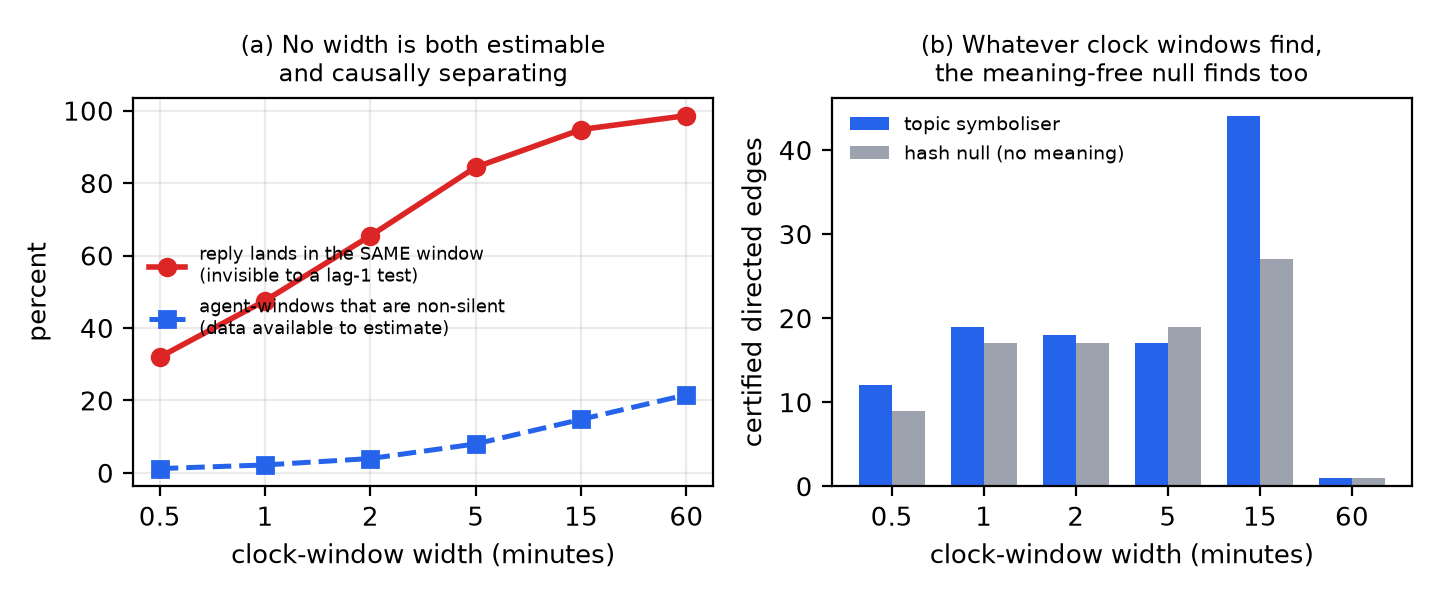
\includegraphics[width=0.92\textwidth]{f1_clock.png}
\caption{Clock-window transfer entropy on the 15 analysed agents of main-village \#general. Left,
the two failure modes as a function of window width. Right, edges certified under the topic
symboliser against the meaning-free hash null.}
\end{figure}

The bind is avoided by ordering messages canonically and letting one message be one tick. Each
agent's series carries its symbol where it spoke and a silent symbol elsewhere, so the lag-1
comparison is between a message and the one immediately before it. The cost is that the measure
captures immediate-predecessor influence only.

\section{The surrogate failure, and two explanations that did not hold}
\label{sec:failure}

An agent is planted into the real stream, drawing its symbols from the channel's marginal and
coupled to nothing at all. It is certified as driving something in 3 of 8 runs when it posts 50
messages, and in 8 of 8 at 100, 263, 600 and 1500 messages, with the mean largest $z$ rising from 5.6
to 12.3, 21.7, 38.3 and 71.7. The error grows with how much the agent speaks, which rules out a
small-sample explanation.

A planted agent could be dismissed as artificial, so the error rate is also measured directly.
Keeping the real speaker sequence and permuting the symbols globally leaves data with no directed
topical influence by construction. The shift surrogate certifies at least one edge in 9 of 10 such
replicates, a family-wise error rate of 0.90 against a nominal 0.05.

\paragraph{What breaks it is the speaker sequence.} Destroying one structure at a time isolates the
cause. Keeping the real speaker order and shuffling only symbols, the shift surrogate fires in 10 of
10 replicates; randomising the speaker order as well drops it to 0 of 10; uniform symbols with the
real order still give 6 of 10. So the driver is the structure of the speaker sequence, not the
symbol distribution and not sparsity. That sequence is far from random in two ways at once: it
repeats a speaker 36\% of the time and returns after one message 38\% of the time, and each agent's
activity is strongly non-stationary, with a median block-share coefficient of variation of 0.79.
Shuffling the order destroys both at once, so this ablation cannot say which of the two mattered.

\subsection{Two explanations I proposed, and the benchmark refuted both}

I initially attributed the failure to mutual exclusivity: only one agent can speak at each tick, so
shifting individual timelines could create overlaps that never occurred in the original
conversation. The benchmark did not support this explanation. A generated channel with exactly one
speaker per tick and steady activity produced an error rate of just 0.025, 95\% Wilson
$[0.011, 0.057]$, far below the 0.90 observed in the real data. Mutual exclusivity alone therefore
cannot explain the failure.

I then suspected turn-taking. In the real channel, speakers repeat 36\% of the time and return after
exactly one message 38\% of the time. However, adding a Markov speaker chain to the generator
produced the opposite result. Turn-taking suppressed the error rather than increasing it. At the
nominal knob values and with no drift the surrogate certified nothing at all across 200 replicates,
while removing turn-taking and introducing drift raised the rate to 0.365. The contribution from
drift was $+0.340$, compared with $-0.025$ for turn-taking. The same inversion appears in the arm
calibrated so that the generated channel reproduces the real channel's measured repeat, return and
block-share statistics rather than merely carrying those numbers as settings: there, turn-taking
alone also certifies nothing, and drift alone gives 0.065.

Neither mechanism, nor their combination in the tested design, reproduced the real-data error rate of
0.90. The largest cell anywhere in the design is 0.365. The real-data ablation removes turn-taking
and non-stationarity together, while the generator separates them. The results point to
non-stationary activity, but the remaining gap means the mechanism behind the full real-data failure
is not yet established.

Every figure above comes from the run at 200 surrogate draws. The first version of this analysis
used 100, which inflates both nulls on the same 2,400 instances: the circular shift fires 53 times
where the 200-draw run does not, against 18 the other way (exact McNemar $p = 3.9 \times 10^{-5}$),
and the permutation surrogate 83 against 20 ($p = 2.7 \times 10^{-10}$). Every qualitative conclusion
in this section is the same at both settings, which is why they are worth stating at all. The
numbers are not, so the draw count belongs in the caption.

\section{The repair, compared}
\label{sec:repair}

Following the local-permutation idea of \citet{runge2018} as adapted by \citet{shorten2021}, each
source keeps its speaking positions and only its symbols are permuted among them. Speaking pattern,
sparsity and turn-taking are preserved exactly, and only the correspondence between symbol and time
is destroyed. On the same destroyed-structure real data the family-wise error rate falls to 0.063
over 300 replicates, 95\% Wilson $[0.041, 0.097]$. The planted uncoupled agent is never certified: 0
of 5 at both 263 and 1500 messages, with mean max $z$ of 2.8 in each case against 22.0 and 68.3
under the shift surrogate.

\begin{figure}[h]
\centering
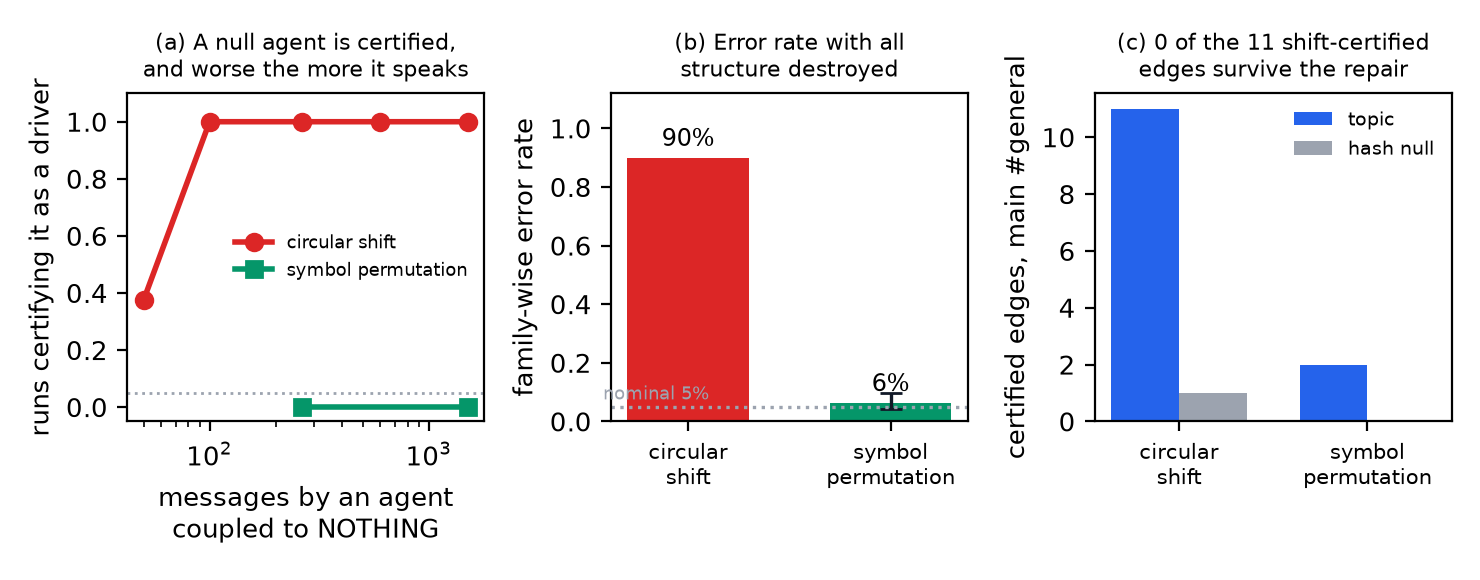
\includegraphics[width=\textwidth]{f2_null.png}
\caption{Left, how often an agent coupled to nothing is certified as a driver, under each surrogate.
Middle, family-wise error rate measured on data with all structure destroyed, with a Wilson
interval; the dotted line is the nominal 0.05. Right, what each surrogate certifies on the real
channel.}
\end{figure}

\subsection{How many surrogate draws are needed}

The number of surrogate draws matters more than I initially appreciated. In a paired comparison of
300 instances, where all four surrogates run on identical symbol grids so the outcomes are paired,
the global permutation surrogate produced a false-positive rate of 0.1167 with 100 draws, falling to
0.0700 with 200 draws, 95\% Wilson $[0.046, 0.105]$. This difference is statistically significant
(exact McNemar $p = 0.0043$). The block-local and Runge local permutations were less sensitive to the
increase: their corresponding rates changed from 0.0900 to 0.0767 and from 0.0967 to 0.0800.

At 200 draws, the global permutation's interval covers the nominal 0.05 and overlaps the real-data
estimate of 0.0633 $[0.0409, 0.0968]$. The real-data result is therefore corroborated rather than
overstated. For practical use, the important point is that reducing the number of surrogate draws
can materially change the result. In particular, the global permutation over-fires at 100 draws by
approximately a factor of two. I would therefore not treat the choice of draw count as a minor
computational detail.

The same correction applies to the benchmark-wide estimate. That figure was 0.0942 at 100 draws.
Repeating all 2,400 instances at 200 draws gives \textbf{0.0679}, 95\% Wilson $[0.0585, 0.0787]$,
and the paired difference is large: 83 instances fire at 100 draws and not at 200, against 20 the
other way, $p = 2.7 \times 10^{-10}$. The conclusion it supports is unchanged, because the interval
still excludes the nominal 0.05. So the permutation repair does carry a residual inflation on clean
generated data, but it is about a third above nominal rather than nearly double.

One limit on this recommendation. I compared 100 draws against 200 and did not test any larger
value, so what the experiment establishes is that 100 is too few, not that 200 is enough. Two
hundred is a lower bound on the draw count rather than a converged setting, and a practitioner whose
conclusions sit near a decision boundary should check their own sensitivity rather than adopt the
number.

\subsection{Choosing a repair, when the error rate cannot choose}

The comparison of the three permutation-based repairs does not produce a clear winner. All four
surrogates were evaluated on identical symbol grids across 300 pure-null replicates, so the
comparison reflects differences between the null models rather than differences between datasets.

\begin{table}[h]
\centering
\begin{tabular}{lrrrl}
\toprule
surrogate & FWER, 100 draws & FWER, 200 draws & 95\% Wilson at 200 & nominal 0.05 \\
\midrule
circular shift                   & 0.0433 & \textbf{0.0333} & $[0.018, 0.060]$ & inside \\
global within-speaker permutation & 0.1167 & \textbf{0.0700} & $[0.046, 0.105]$ & inside \\
block-local permutation          & 0.0900 & \textbf{0.0767} & $[0.052, 0.112]$ & excluded \\
local permutation \citep{runge2018} & 0.0967 & \textbf{0.0800} & $[0.054, 0.116]$ & excluded \\
\bottomrule
\end{tabular}
\caption{Four surrogates on identical symbol grids, 300 pure-null replicates, at both draw counts.}
\end{table}

At 200 draws, paired on the same 300 instances, the circular shift is not significantly different
from the global permutation ($p = 0.0614$), although it differs from block-local permutation
($p = 0.0294$) and from Runge's local permutation ($p = 0.0201$). At 100 draws it differed from all
three, which is the draw-count artifact again. The three repairs remain statistically
indistinguishable from one another, with pairwise $p$-values of 0.85, 0.65 and 1.00. The apparent
differences in their error rates are not sufficient to establish a ranking.

Choosing between them therefore requires more than calibration, and two readings pull against each
other. Runge's local permutation has the strongest methodological justification for preserving the
structure it is intended to preserve, and it follows the approach adapted to event data by
\citet{shorten2021}. Block-local permutation is more heuristic and introduces a free parameter that
has not been tuned. Global permutation is the simplest. On the other hand, the global permutation has
the most favourable interval relative to the nominal rate, and is the only repair that costs nothing
measurable against the shift on clean stationary data, although neither difference is statistically
established. I do not consider the observed error rates sufficient to select one repair over the
others. The choice should be guided by the structure the null is intended to preserve and the
assumptions that can be justified for the data.

\subsection{When to use the repair}

A drift sweep gives the practical reading. Across 150 replicates per cell at 200 surrogate draws,
the circular shift degrades steadily as activity drift increases while the three repairs do not.

\begin{table}[h]
\centering
\begin{tabular}{lrrrr}
\toprule
activity drift & circular shift & global permutation & block-local & local \\
\midrule
0.0 & \textbf{0.013} & 0.093 & 0.080 & 0.093 \\
0.3 & 0.100 & 0.100 & 0.093 & 0.120 \\
0.6 & \textbf{0.193} & 0.053 & 0.047 & 0.067 \\
0.9 & \textbf{0.380} & 0.087 & 0.080 & 0.080 \\
\bottomrule
\end{tabular}
\caption{Family-wise error on pure nulls as activity drift increases, 150 replicates per cell, 200
surrogate draws. Every certified edge is a false positive by construction.}
\end{table}

The pattern is supported by a formal trend test rather than by eye. A Cochran-Armitage test across
the four ordered drift levels gives the circular shift $z = 8.667$, $p < 10^{-15}$, and gives every
repair nothing: $p = 0.51$ for the global permutation, 0.63 for block-local and 0.37 for local. The
same pattern holds at both surrogate draw counts, so it does not depend on that choice.

The repairs are therefore flat under drift rather than calibrated. Only one of the four global
permutation intervals covers the nominal 0.05, and the rest sit nearer 0.09, so what the repair buys
is insensitivity to drift rather than correctness. One asymmetry should be stated rather than
hidden: block-local covers nominal in three of the four cells where the global repair covers one.
The two remain pairwise indistinguishable, so this is not grounds to switch the recommendation, but
it does mean the global repair cannot be described as the best-calibrated under drift.

The results also show why the repair should not be treated as universally preferable. At zero drift
the circular shift has an error rate of 0.013, while the three repairs are all around 0.08 to 0.09.
That advantage is gone by the first drift step: at drift 0.3 the shift reads 0.100 against the global
permutation's 0.100 and block-local's 0.093, so the crossover falls between drift 0.0 and 0.3 rather
than at some higher level. By drift 0.6 the shift is roughly four times the repairs. If a channel has
been checked and found stationary, the circular shift may be sufficient. When activity is
non-stationary the repairs are the more stable choice, and the margin for error on that judgement is
narrow, because the crossover arrives by the first drift level tested.

\section{Continuous time, and what the repair cannot test}

An earlier analysis identified continuous-time estimation as the principled option for event data
but did not evaluate it. Running the continuous-time estimator CoTETE on both channels certifies 0
edges in either case, compared with 2 for main-village and 18 for open-chat under the discrete,
turn-ordered analysis. Its highest $z$-scores are 3.062 and 3.980, below the respective max-T
thresholds of 4.171 and 4.308.

At first these results might appear to contradict the symbol-based analysis. The two estimators
operate on different information, however. CoTETE's public API takes event times with no symbol
channel, while the transfer-entropy analysis here uses topic symbols. To test whether this
difference explains the results, I reduced the data to timing alone, replacing every spoken symbol
with the same code. Under this representation the estimator used here also detects 0 edges in both
channels, matching CoTETE. Using the circular-shift surrogate instead produces 12 and 3 edges. So
neither method detects relationships from event timing alone in these channels, and the edges found
by the symbol-based analysis depend on symbol correspondence, which the continuous-time estimator
cannot access.

Two caveats attach to those $z$-scores, and the second attaches to the larger of them. Point
estimates from this estimator are stochastic to about 17\% across repeated runs, so none of these
values should be read to more than two significant figures. And open-chat's highest $z$, the 3.980,
belongs to the one pair whose surrogate draws mostly failed: it needed 1,936 failed draws to obtain
100 successes, a 4.9\% success rate. Those surrogates are conditioned on being estimable, so that
pair's null is biased in an unknown direction. The conclusion does not rest on it, since that pair
falls below threshold and so does every other pair, but the number should not be quoted as a clean
measurement. The failures themselves were a defect rather than a property of the data: an enlarged
exclusion window can empty the neighbour search on sparse bursty event trains and raise an error
that terminates a whole pair, with no handling at the public entry point. This has been reported
upstream.

There is also a fundamental limitation in applying the recommended permutation surrogate to
timing-only data. When every event carries the same symbol, permuting those symbols changes nothing.
The observed statistic and the surrogate null are identical, making the test exactly degenerate:
standard deviation 0 across all 210 pairs and $p = 1.0$ everywhere. \textbf{The repair has zero power
against timing structure by construction.} The permutation surrogate is appropriate for testing
relationships in the symbol sequence, but it does not answer whether relationships exist in event
timing. These are different questions, and choosing one null means giving up the ability to test the
other with that procedure.

\section{Confounding, and what conditioning removes}

A valid surrogate fixes calibration but not confounding. If every agent tracks a drifting channel
topic, every pair is genuinely dependent through the channel, and pairwise transfer entropy cannot
tell that from direct influence. I therefore also report a \textbf{conditional} estimate, which asks
whether a source's last message adds anything about a target's next one beyond the target's own
history and the channel's recent state. The conditioning variable is the modal symbol of the last
twelve messages, excluding the immediately preceding one so that it does not simply restate the
source.

On a generated benchmark whose decisive instances contain no influence while every agent tracks a
shared drifting topic, so that any certified edge is common cause, pairwise transfer entropy
certifies \textbf{22.3} edges on average and conditioning takes that to \textbf{0.33}, lifting pooled
precision on the four-edge instances from 0.17 to \textbf{0.80} at a recall of 1.0 either way. Across
couplings from 0.05 to 0.8 the conditional test still finds the planted edge in 3 of 3 runs, so the
gain costs no power.

The benchmark flatters the conditional estimator, since its common cause is a shared modal topic and
the conditioning variable is the channel's modal topic. The real channels are harder, and
conditioning there costs degrees of freedom: a 9-symbol alphabet with a 9-valued context gives 6,561
cells against about 7,900 ticks, so that variable is also coarsened to 4 and 2 values.

\begin{table}[h]
\centering
\begin{tabular}{lrrrr}
\toprule
channel & pairwise & conditional, 9 values & 4 values & 2 values \\
\midrule
main \#general      & 2  & \textbf{2, the same two edges} & 2 & 3 \\
open-chat \#general & 18 & \textbf{0} & \textbf{7} & \textbf{13} \\
swarm, room a       & 1  & \textbf{0} & & \\
\bottomrule
\end{tabular}
\caption{Conditioning at three resolutions. Main-village's two edges are robust to that choice;
open-chat's zero is not.}
\end{table}

At the finest resolution the open-chat test is degenerate, its surrogate sitting above the observed
statistic for 65\% of pairs with the largest $z$ in the family only 4.4, so it is failing to reject
rather than finding nothing to reject. Open-chat's structure therefore remains
\textbf{undetermined}: depending on the conditioning resolution, between 0 and 13 of its 18 edges may
survive. That resolution is a free parameter an analyst would set once and never revisit. This is a
property of the channel rather than the estimator: on structure-free real data the conditional test
fires in 2 of 40 replicates, an error rate of 0.05 with a mean $z$ of $-0.001$, so it is nominal
rather than conservative.

\section{The symbolisation floor}
\label{sec:floor}

Everything these methods produce is downstream of turning text into symbols. On the benchmark, where
the underlying topics are known, detection performance drops sharply when agreement between the
symboliser and the ground truth falls below roughly ARI 0.44, and this behaviour appears across the
tested estimators. Importantly, the false-positive rate can look \emph{better} below this point,
because the shared topic structure needed to produce confounded detections is no longer represented
reliably. A pipeline that stops detecting relationships may therefore have lost the signal it needs
rather than become more reliable, and nothing downstream of the symboliser can tell those apart.

\subsection{Detecting the floor without labels}

That degradation can be detected without ground-truth labels. Across the nine-level benchmark sweep,
three statistics separate the below-floor cases with zero errors: seed stability at a threshold of
0.623, agreement with LSA at 0.646, and the Calinski-Harabasz index at 138.9. Seed stability here is
the \textbf{minimum} pairwise agreement across seeds, not the mean; the mean variant makes one error,
at a different threshold of 0.791. Silhouette has the strongest correlation with true ARI, at 0.979,
but is not useful for identifying the boundary because its threshold falls within a gap of just
0.002. A statistic that tracks clustering quality most closely is not necessarily the best one for
making a classification decision.

Error count cannot choose among the three that were perfect, so I tested whether each threshold still
means what it meant when the channel changes for reasons other than topic separability. Applying each
cut unchanged to thirty cells that vary turn-taking, drift, agent count, volume skew, message length
and corpus size, twenty-seven of which hold true ARI at exactly 1.000:

\begin{table}[h]
\centering
\begin{tabular}{lrrrr}
\toprule
diagnostic & cut & errors where fitted & errors, nuisance set & of those at true ARI 1.000 \\
\midrule
seed stability, min across seeds & 0.623 & 0 & 2 & \textbf{0} \\
LSA agreement                    & 0.646 & 0 & 2 & \textbf{0} \\
Calinski-Harabasz                & 138.9 & 0 & 6 & \textbf{3} \\
\bottomrule
\end{tabular}
\caption{Whether a cut fitted on the vocabulary-overlap mechanism survives a change in the channel
that is not a change in topic separability.}
\end{table}

The two bounded statistics err only on the short-message cells, where the symbolisation genuinely has
degraded. Calinski-Harabasz additionally condemns all three cells whose true ARI is exactly 1.000,
for no reason beyond the corpus holding 2,000 messages rather than 8,000, where it reads 76 to 77
against its own cut of 138.9. It is unbounded and grows with sample size, so a published numeric
threshold for it carries no meaning on another corpus. That is why I recommend the two bounded
statistics and not the index that matched them on error count. \textbf{A cut that moves with the
corpus is not a floor cut.}

This is not a weak statistic being discarded on a technicality. Calinski-Harabasz correlates with
true ARI at 0.973, almost as closely as silhouette, and unlike silhouette it classifies the floor
perfectly where it was fitted. It still cannot carry a published threshold. That is the sharper form
of the point above: neither the statistic that tracks quality most closely nor the one that
classifies best on the fitting mechanism is necessarily the one whose cut another researcher can
reuse.

There are important limits to this result. The effective sample size is nine rather than 54, because
the classification label is determined by overlap level. There are no observations between ARI 0.444
and 0.222, so the exact location of the boundary within that interval remains unknown. These
diagnostics classify whether a result is below the tested detection floor; they do not estimate ARI,
and their behaviour is flat between 0.68 and 1.00, and not even monotone there. The benchmark also
uses a single degradation mechanism with a known and correct value of $k$, whereas the true number of
topics in real conversations is unknown. I therefore treat 0.44 as a benchmark-specific, bracketed
result rather than a universal threshold.

\subsection{A contradiction the diagnostic lost}

I initially used these diagnostics to classify one real channel, open-chat, as below the
symbolisation floor. That conclusion did not agree with the channel's measured results: open-chat
certified 18 and 22 edges under the two symbolisers, compared with 2 and 1 for main-village, and its
hash-based null certified zero edges. Rather than treating this disagreement as evidence that the
original measurements were wrong, I revisited the diagnostic itself.

The problem was the choice of $k$. Repeating the comparison with the same channels, loader and window
reproduced the published $k=8$ results to the digit. At $k=4$, however, open-chat reached stability
scores of 0.950 and 0.978, the highest values produced by either channel across the tested settings,
and both exceeded the diagnostic thresholds. The earlier below-floor classification was therefore a
conclusion about one arbitrary choice of $k$, not a reliable statement about the channel. Message
length does not explain the difference either: 27.1\% of main-village messages contain fewer than
five tokens, compared with 2.3\% in open-chat, so the short-message channel is the one the diagnostic
cleared.

This correction changes how the symbolisation results should be read, and it withdrew three claims.

\begin{enumerate}
\item \textbf{The claim that no topic signal remains below the floor is too strong.} The
circular-shift surrogate recovers all four planted edges at every tested overlap level, including
0.95, where ARI is 0.011. The observed collapse is in the permutation null, not necessarily in the
underlying data.
\item \textbf{ARI 0.44 cannot be treated as a universal detection threshold.} When the shared-topic
parameter is 0, detection continues down to ARI 0.296, so the boundary depends on both the
symboliser and the channel.
\item \textbf{Edge counts cannot be used as a measure of symboliser quality.} Even at ARI exactly
1.000, changing the shared-topic parameter alone moves the permutation edge count from 5 to 78.
\end{enumerate}

The diagnostics also do not transfer reliably outside the mechanism on which they were evaluated.
Their balanced accuracy falls from 1.00 to 0.75 and 0.571 under a known mismatch in $k$. All seven
errors made by seed stability are false below-floor classifications, and in every one of those cases
the detector still identifies all planted edges; of the fourteen cells it condemned, eleven had full
conditional recall. The failure direction is the dangerous one: it condemns working symbolisations.

This was an important correction to my own interpretation. I introduced a diagnostic to check whether
the symbolisation was reliable, applied it to the real channels, and found that it contradicted
measurements already in hand. Investigating that contradiction showed the diagnostic was sensitive to
an arbitrary modelling choice. The result is not that the original measurements were wrong, but that
the control was being asked to support a broader conclusion than the evidence allowed. These
diagnostics remain useful within their tested setting, and \textbf{no channel-level floor verdict
should be issued from a single $k$}.

\section{The benchmark}

Real logs have no ground truth, so the common-cause question could not be settled on them. The
generator used here makes the influence graph known by construction: it decides, in code, who speaks
at which tick, on which topic, and who reacts to whom. Surface text is a separate, replaceable layer
drawn from disjoint per-topic vocabularies, so the whole thing runs offline and a detector still has
to symbolise raw text rather than read the labels. Turn-taking and activity drift are independent
knobs, so the two can be varied one at a time, and the generator reproduces its earlier behaviour
bit for bit when both are zero.

\benchname{} is released with 150 tests covering the generator, the detector harness, the text layer,
the floor analysis and the turn-taking factorial.
\ifdeanon{Code and benchmark:
\url{https://github.com/manunicholasjacob/swarm-influence-bench} and
\url{https://github.com/manunicholasjacob/swarm-influence-audit}.}{Code and benchmark are publicly
released; the links are withheld here for anonymity and will be given in the camera-ready version.}

One property of the benchmark must be stated when its numbers are quoted. Planting an edge displaces
other agents' speaking turns, so the generated instances contain real lag-1 dependencies that the
label set does not list. Precision measured against those labels is therefore a \textbf{lower bound}
for any detector, and what the benchmark supports is the comparison between two estimators rather
than the absolute value of either.

\section{What an overseer should do}

Six inexpensive controls should be included whenever an influence graph over an agent channel is
published.

\begin{enumerate}
\item \textbf{Plant an agent coupled to nothing, at your channel's volumes, and check it is not
certified.} This one test would have caught the failure reported here, at one run per volume.
\item \textbf{Measure the error rate directly}, by destroying the structure your method claims to
find and checking the family-wise rate is near nominal. If it is not, your surrogate does not match
your data.
\item \textbf{Preserve the speaker sequence in your surrogate.} Any surrogate that moves an agent's
messages in time will disturb it, and \citet{shorten2021} is the principled route. Use at least 200
surrogate draws, because at 100 the global within-speaker permutation over-fires by roughly a factor
of two.
\item \textbf{Establish the detection floor before interpreting an absence.} ``No edges'' and ``no
influence'' are different claims.
\item \textbf{Condition on the channel, report both numbers, and sweep the resolution.} Pairwise and
conditional bound the answer, and the gap between them is the result. Conditioning costs cells, so
check whether your answer is an artifact of how finely you conditioned. On one channel here it was.
\item \textbf{Report how well your symboliser agrees with the truth, on data where you know it.}
Everything is downstream of turning text into symbols, and below roughly ARI 0.44 detection
collapses whatever the estimator. I have found this control in no influence-detection paper, and it
is also the one that cannot be run on real logs, which is why the floor remains the largest
unquantified threat here.
\end{enumerate}

Two habits follow: publish a meaning-free null's count beside the real one, and require held-out
replication before calling a graph a structure.

\section{The real channels, and what survives}

Re-running every channel under the repaired surrogate changes the answers, and not in one direction.

\begin{table}[h]
\centering
\begin{tabular}{lrrr}
\toprule
channel & window messages & shift: topic / hash & permutation: topic / hash \\
\midrule
main \#general      & 8,800 & 11 / 1 & 2 / 0 \\
open-chat \#general & 8,226 & 3 / 0  & 18 / 0 \\
swarm, room a       & 3,846 & 2 / 1  & 1 / 0 \\
\bottomrule
\end{tabular}
\caption{The same channels under both surrogates, with the meaning-free hash null beside each.}
\end{table}

In main-village, \textbf{none} of the 11 edges the standard recipe certifies survives the repair, and
the two the valid surrogate certifies were not among them. In open-chat the correction runs the other
way, 3 edges becoming 18, because pathological pairs inflate the max-T threshold and raise the bar
for everything else. An invalid surrogate does not simply add false positives; it scrambles the
result.

Main-village's two edges are the strongest thing here and they are still not a finding, because they
do not replicate: the adjacent fourteen-day window certifies nothing at all under either estimator.
Given the detection floor, that silence is as consistent with the test sitting near its limit as with
the edges being absent, and the two cannot be separated. Power is governed by how much an agent says
as much as by how strongly it copies, and it is channel-specific: in main-village a planted follower
copying on 80\% of its messages is caught only 1 time in 4, while in open-chat one copying 10\% of
the time is caught 3 times in 4. Replication is weak everywhere: under the standard recipe the
adjacent window shares 1 edge out of 8 and 4, and that edge is also the only one the hash null
certifies. No certified edge in this work replicates out of sample.

\begin{figure}[h]
\centering
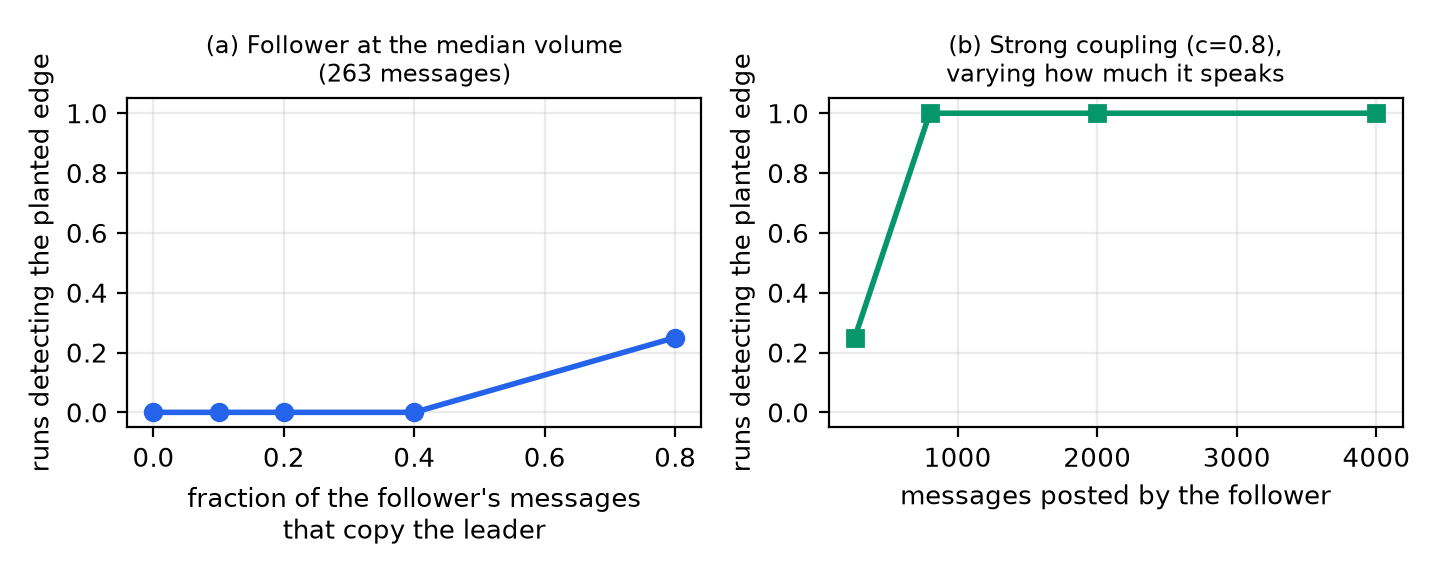
\includegraphics[width=0.92\textwidth]{f4_power.png}
\caption{Detection of a planted follower under the repaired surrogate. Left, varying the fraction of
its messages that copy the leader, at the median agent's volume. Right, varying how much it speaks,
at strong coupling.}
\end{figure}

\paragraph{Humans in the channel.} Main-village \#general is now effectively human-free, with 3 human
messages in the window, so the question has to be asked in open-chat, where 32\% of messages come
from 124 human visitors. Pairwise, with humans collapsed into one node, 19 edges are certified.
Conditioning removes almost all the agent-to-agent structure and little of the rest: \textbf{four
edges survive, of which three run from humans to agents, one is agent to agent, and none run from an
agent to a human.} The asymmetry is not an artifact of the confound. It should be read carefully all
the same: topical dependence from a person to an agent is also what ordinary responsiveness looks
like, so the measurement supports only that the dependence is dyad-specific and directional, not
that anyone is steering a swarm.

\section{Reproducibility, and one limitation of it}

Every number in this paper is recomputed from committed analysis output by a verifier that fails on a
mismatch, and that verifier covers the prose of this paper as well as the figures.

One limitation should be stated plainly. Re-running the counts in the earlier stationarity sweep with
the same seeds and configuration, only one of the eight cells reproduced exactly; the remaining
differences were one or two replicates per cell. Seven of the eight published rates still fell within
the recomputed Wilson intervals, and no conclusion changed. The exception is the zero-drift cell under
the permutation null, where the published 1 of 30 falls just below the recomputed interval of
$[0.035, 0.256]$ for 3 of 30, and no result here depends on that cell.

The generator, estimator and BLAS configuration were investigated and ruled out as the source. The
most likely explanation is a library-level difference, particularly in scikit-learn's $k$-means
implementation within the symboliser, whose output can vary between versions. Every sweep now records
the environment it ran under: Python 3.14.6, numpy 2.5.1, scipy 1.18.0 and scikit-learn 1.9.0,
including the BLAS build and the number of BLAS threads each worker used.

This does not make the previously published counts exactly reproducible. It provides a more clearly
specified environment in which subsequent results can be checked. For that reason I report rates
alongside their confidence intervals rather than exact replicate counts. The distinction between
reproducing a result within its uncertainty and reproducing every individual count matters, and only
the first is claimed.

\section{Conclusion}

Applied to real agent chat, the standard recipe for ``who drives whom'' needs repair before it says
anything. Clock windows cannot separate a message from its answer at the speed agents reply, and what
they certify is matched by a null with no access to meaning. The turn-ordered grid that fixes this
breaks the circular-shift surrogate: family-wise error 0.90 against a nominal 0.05, caused by the
speaker sequence itself. Restricted permutation surrogates repair most of that, but they are flat
under drift rather than calibrated, they are mutually indistinguishable at this precision, and one of
them needs twice the surrogate draws anyone would think to use. A valid surrogate fixes calibration
but not confounding. What survives is small: two dyad-specific edges that do not replicate, an
undetermined answer set by conditioning resolution, and influence running from people into agents and
never back. \textbf{An influence graph should not guide decisions until its error rate, its confound,
its detection floor and its symboliser's fidelity are reported.}

\section*{Limitations}

\begin{itemize}
\item \textbf{Immediate-predecessor only.} The turn-ordered lag-1 measure sees influence from the
message directly before a reply. Influence acting over several turns, or through a room's accumulated
context, is out of scope.
\item \textbf{Discrete approximation to an event process.} Agent chat is event-based in continuous
time. The turn-ordered discretisation with a permutation surrogate is a practical fix, and the
continuous-time comparison above shows what that choice gives up.
\item \textbf{The mechanism behind the real 0.90 is not established.} The generator separates
turn-taking from drift and points at drift, but the largest cell anywhere in the design is 0.365.
\item \textbf{Symbolisation quality cannot be measured on the real logs.} The central result survives
an independent symboliser, but the edge count does not: it moves with alphabet size and with which
messages the topic model is fit on. The floor remains the largest unquantified threat.
\item \textbf{No ground truth in the real logs.} The validity argument rests on planted controls and
on the meaning-free null, not on recovering a known answer.
\item \textbf{Conditioning removes real influence too.} The conditional estimate discards influence
that works by shifting what the channel is talking about, which in a group chat may be a large part
of genuine influence. It is a lower bound on dyadic influence.
\item \textbf{The human result is exploratory.} It rests on one village and one window and should be
read as a lead.
\end{itemize}

\section*{Broader impact and ethics}

This work audits influence detection on a population of AI agents, which is dual-use. Used
defensively it helps an overseer decide what an influence graph is worth, and the main result is
deflationary: it tells practitioners to trust these outputs less, which reduces rather than increases
the chance of acting on a bad attribution. The same tooling could be used to identify the most
influential agent in a swarm in order to target it, or to surveil participants in a channel. Three
properties limit the misuse. The subjects are AI models; the dataset is already public under research
terms and no re-identification is added; and the measure is weak and local, recovering
immediate-predecessor topical dependence rather than any model of how to steer an agent.

The dataset's research terms were followed: research use only, no training on the data, no
re-identification, citation of the source, and notification of the authors of resulting publications.
Human participants appear only as an aggregate node or as anonymised visitor labels, never by name or
handle, and no content attributable to an individual person is reported. Message text and metadata
were read, never model weights or private user data.

The use of a large language model in this work is disclosed in the first-page footnote, as TMLR
requires.

\bibliographystyle{tmlr}
\bibliography{refs}

\end{document}
"               camera-ready
% Use build.py, which runs all of them and checks the anonymous output for leaks.
\providecommand{\TMLRMODE}{submission}
\makeatletter
\def\@tmlrpreprint{preprint}
\def\@tmlraccepted{accepted}
\ifx\TMLRMODE\@tmlrpreprint
  \usepackage[preprint]{tmlr}
\else
  \ifx\TMLRMODE\@tmlraccepted
    \usepackage[accepted]{tmlr}
  \else
    \usepackage{tmlr}
  \fi
\fi
\makeatother

\usepackage{hyperref}
\usepackage{url}
\usepackage{booktabs}
\usepackage{graphicx}
\usepackage{amsmath}

% Gate every identifying string on whether identity may be revealed at all. The flag to test is
% \if@accepted, NOT \if@preprint: tmlr.sty's [preprint] option sets BOTH, so \if@accepted is true
% for the preprint and the camera-ready and false only for the anonymous submission, which is
% exactly the condition wanted. Gating on \if@preprint alone also hid the repository URLs from the
% camera-ready, which is where this paper promises to give them. \if@accepted is internal to
% tmlr.sty, hence the \makeatletter. The anonymous build takes the second argument.
\makeatletter
\newcommand{\ifdeanon}[2]{\if@accepted#1\else#2\fi}
\makeatother
\newcommand{\benchname}{\ifdeanon{SwarmInfluence-Bench}{the benchmark}}

% An unmarked footnote, for the LLM-use disclosure. TMLR's FAQ requires the disclosure and names
% the location: authors must "mention explicitly in their submission that they have used this
% tool", "as a footnote on the first page". Verified against jmlr.org/tmlr/faq.html on 10 Nov 2026.
% It is therefore not optional, and it does not belong in Broader Impact, where it sat until now.
% Nothing in the policy asks for the vendor's name, so none is given.
\newcommand{\disclosurefootnote}[1]{%
  \begingroup\renewcommand\thefootnote{}\footnote{#1}\addtocounter{footnote}{-1}\endgroup}

\title{An Influence Graph Over AI Agents Certifies an Agent That Copies Nobody}

% Hidden by the tmlr package unless [accepted] or [preprint] is given.
\author{\name Manu Nicholas Jacob \email manunicholasjacob@gmail.com \\
        \addr Independent Researcher}

\def\month{11}
\def\year{2026}
\def\openreview{\url{https://openreview.net/forum?id=XXXXXXXXXX}}

\begin{document}
\maketitle

\begin{abstract}
Circular-shift surrogates can produce severely inflated false-positive rates when applied to
turn-ordered multi-agent conversations, reaching a family-wise error rate of 0.90 against a nominal
0.05. A generated benchmark separates two candidate mechanisms and points at non-stationary speaker
activity rather than turn-taking, which suppresses the failure rather than causing it. No setting of
either knob reproduces the observed 0.90, however, so what drives the full real-data failure remains
open. Restricted permutation surrogates substantially reduce the problem. Their error rate is flat
with respect to drift rather than at the nominal level, and for the global within-speaker variant it
depends on how many surrogate draws the null is built from. Calibration alone does not address
confounding, which motivates a conditional estimator validated against a benchmark with planted
ground truth. I also identify a symbolisation-dependent detection limit and develop label-free
diagnostics for it, and show that their calibration does not transport across degradation
mechanisms. The benchmark is released.
\end{abstract}

\disclosurefootnote{\textbf{Use of a large language model.} A large language model was used as an
assistive tool: to help write and run the analysis code, and to help draft this paper. The author is
responsible for every claim, number and figure. All results come from the released code run on the
public dataset, no result or reference is fabricated, and every number in this paper is recomputed
from committed analysis output by a verifier that fails the build on a mismatch.}

\section{Introduction}

When AI agents interact in a shared channel, it is useful to understand how they influence one
another. Information-theoretic methods offer a way to measure this through lagged transfer entropy,
surrogate testing, and per-agent influence scores. They are attractive because they require no
labels and no access to model internals, only a record of who said what and when. The reliability of
those measurements is what this paper examines.

Almost every demonstration of these detectors runs on synthetic traces with a planted leader, where
the analyst controls timing and vocabulary. Real agent chat is asynchronous, bursty, and written in
open language. The narrower question here is whether the standard recipe, applied to real agent
logs, returns anything an overseer should act on.

The audit runs on the AI Village corpus \citep{aidigest2026}, in which frontier models share chat
channels over eighteen months across four villages differing in size, lifetime and tempo, applying
the checks a reader should demand: planted controls, a meaning-free symboliser, replication in a
held-out window, and sensitivity to every parameter that had to be chosen.

\begin{enumerate}
\item The conventional circular-shift surrogate is \textbf{invalid} on turn-ordered agent chat: a
family-wise error rate of 0.90 against a nominal 0.05, caused by the structure of the speaker
sequence itself.
\item Restricted permutation surrogates restore most of the calibration, and re-certifying under one
\textbf{scrambles rather than shrinks} the answer: one channel loses all 11 of its edges, another
gains 15.
\item The three restricted variants are \textbf{mutually indistinguishable} at the precision reached
here, so the choice between them cannot be justified on error rate. The global within-speaker
variant additionally needs on the order of 200 surrogate draws, and over-fires by roughly a factor
of two at 100.
\item Calibration is not confounding, so a conditional estimate is added and validated on a released
benchmark with a known influence graph: common-cause false edges fall from 22.3 to 0.33, and on the
planted-edge instances precision rises from 0.17 to 0.80 with no loss of recall or power.
\item The same benchmark exposes a \textbf{symbolisation floor}. Below roughly 0.44 adjusted Rand
index between symboliser and truth, detection collapses whatever the estimator. Label-free
diagnostics detect that floor, but their calibration does not transport across degradation
mechanisms, and I report where it fails.
\item On the real channels two edges stand at every conditioning resolution, 18 are
\textbf{undetermined} between 0 and 13, none replicates out of sample, and what survives alongside
humans runs from people to agents.
\end{enumerate}

\section{Related work}

\paragraph{Transfer entropy and surrogates.} Transfer entropy \citep{schreiber2000} measures how much
a source's past reduces uncertainty about a target's next symbol beyond the target's own past.
Plug-in estimators are biased upward on short series, so significance rests on surrogate data, with
family-wise error controlled by a max-T test \citep{westfall1993}. The usual surrogate is a circular
time shift of the source.

\paragraph{Event-based data breaks the shift surrogate.} \citet{shorten2021}, on neural spike trains,
show that the conventional source-time-shift surrogate fails to represent the null hypothesis of
conditional independence for event-based processes, and adapt to that setting the nearest-neighbour
local permutation scheme of \citet{runge2018}. Agent chat is event-based in that sense: messages are
events in continuous time, not samples of a clocked signal. The correction is not a contribution of
this paper. The contribution is showing that the same failure carries over to multi-agent safety
monitoring, and that it can be severe enough to create apparent leaders where none exist.

\paragraph{The same failure, concurrently, in multi-agent reinforcement learning.}
\citet{papadopoulos2026} report a closely related surrogate failure in multi-agent
reinforcement-learning action series. Their agent pairs have zero influence by construction, yet
circular time shifts produce false-positive rates of 100\% and 98.2\% against a nominal 0.05. A
plain permutation surrogate fares no better in their setting, at 100.00\% and 99.95\%. Their
proposed correction restricts permutations to blocks of training time, which returns the rates to
5.25\% and 5.50\%.

There are important differences between their setting and this one. Their data consist of binary
actions recorded over twelve thousand training rounds, whereas these data are symbolised
natural-language messages arranged on a turn-ordered conversational grid. Their non-stationarity
comes from monotone drift associated with annealing exploration; here the relevant non-stationarity
appears in the speaker sequence. Neither result should be taken as a direct extension of the other.

Nevertheless, the fact that both approaches rely on restricted permutations is worth noting. Their
permutation blocks are defined by training time, while mine are defined by an agent's own speaking
positions. This provides convergent evidence that unrestricted temporal rearrangement can be
problematic in non-stationary multi-agent data. Their findings also serve as a useful warning for
the approach taken here, and the warning has a measured form rather than a rhetorical one: in their
data the unrestricted permutation failed as completely as the time shift, at 100.00\% against a
nominal 0.05. Permutation-based surrogates are not automatically protected against
non-stationarity, and what protects the one used here is the restriction, not the permutation. I
claim no priority over their result and view the two studies as complementary, addressing different
forms of structured multi-agent data.

\paragraph{Oversight under a budget.} AI-control research frames monitoring as resource constrained,
with a cost for false positives \citep{greenblatt2024}. An influence graph is one such measurement,
and its error rate is the concern here.

\paragraph{Clustering stability.} The idea of using clustering stability as a label-free quality
indicator is not new. It has a substantial history, including \citet{benhur2002},
\citet{lange2004}, von Luxburg's review of clustering stability \citep{vonluxburg2010}, and
\citet{tibshirani2005} on prediction strength. What is different in Section~\ref{sec:floor} is the
calibration of these diagnostics against a detection-performance floor rather than against cluster
recovery alone.

\section{Data and representation}

The AI Village dataset ships one gzipped-JSONL table per village. Four villages are used, differing
enough to test whether any finding is a property of one channel.

\begin{table}[h]
\centering
\begin{tabular}{lrrrrl}
\toprule
village & agent messages & agents & lifetime & human messages & busiest room \\
\midrule
main      & 205,726 & 58  & 576 days & 10,029 & \#general (166,715, 81\%) \\
open-chat &  35,483 & 23  &  66 days & 12,264 & \#general (all) \\
swarm     &   3,848 & 133 &   1 day  &      5 & room a (3,846) \\
game-jam  &     838 & 6   &   3 days &     36 & per-team rooms \\
\bottomrule
\end{tabular}
\caption{The four villages. A 2026 scaffolding change scopes each agent to its current room's
context, so the busiest room of each village is a self-contained influence substrate and is analysed
alone.}
\end{table}

The primary window is the final fourteen days of main-village \#general, 17 to 31 October 2026,
holding 8,800 agent messages. Twenty-two models posted at least 50 messages each and the directed
test uses the 15 busiest, giving 7,958 message events. Two scaffolding facts are disclosed rather
than corrected: the automated nudger was off throughout, and the unused \#best and \#rest rooms were
soft-deleted mid-window, which does not touch \#general.

\subsection{From open language to symbols}

Transfer entropy needs discrete symbols, so each message is mapped to a small alphabet before
influence is estimated, and that mapping is kept separate from the estimator. A topic symboliser
(TF-IDF then $k$-means, $k=8$) gives a message its topic cluster id, so paraphrases of one idea share
a symbol. A hash symboliser, a stable hash of the normalised text into $k=8$ buckets, has no notion
of meaning and serves as a null: an edge appearing under both lives in timing alone.

\subsection{The lag problem, and why clock windows cannot solve it}

A lag-1 transfer entropy compares window $t-1$ with window $t$, so influence landing inside one
window is invisible to it. Agent chat makes this binding. Among the fifteen analysed agents the gap
between consecutive messages by different speakers has a median of 28.1 seconds (25th percentile
9.2, 75th 66.2, 95th 159.3), so turn-taking is a seconds-scale process while any clock window wide
enough to hold two speakers is minutes wide and swallows both a message and its answer.

Both horns are measurable. At 30 seconds only 1.2\% of agent-windows hold a message, while 32.0\% of
replies already land in the same window as what they answer, rising to 84.4\% at five minutes. At
every width tried, the meaning-free hash null certifies comparably many edges, and more at five
minutes: 9 against 12 at thirty seconds, 17 against 19 at one minute, 27 against 44 at fifteen, and
19 against 17 at five. Whatever clock-window transfer entropy was detecting there, it was not shared
meaning.

\begin{figure}[h]
\centering
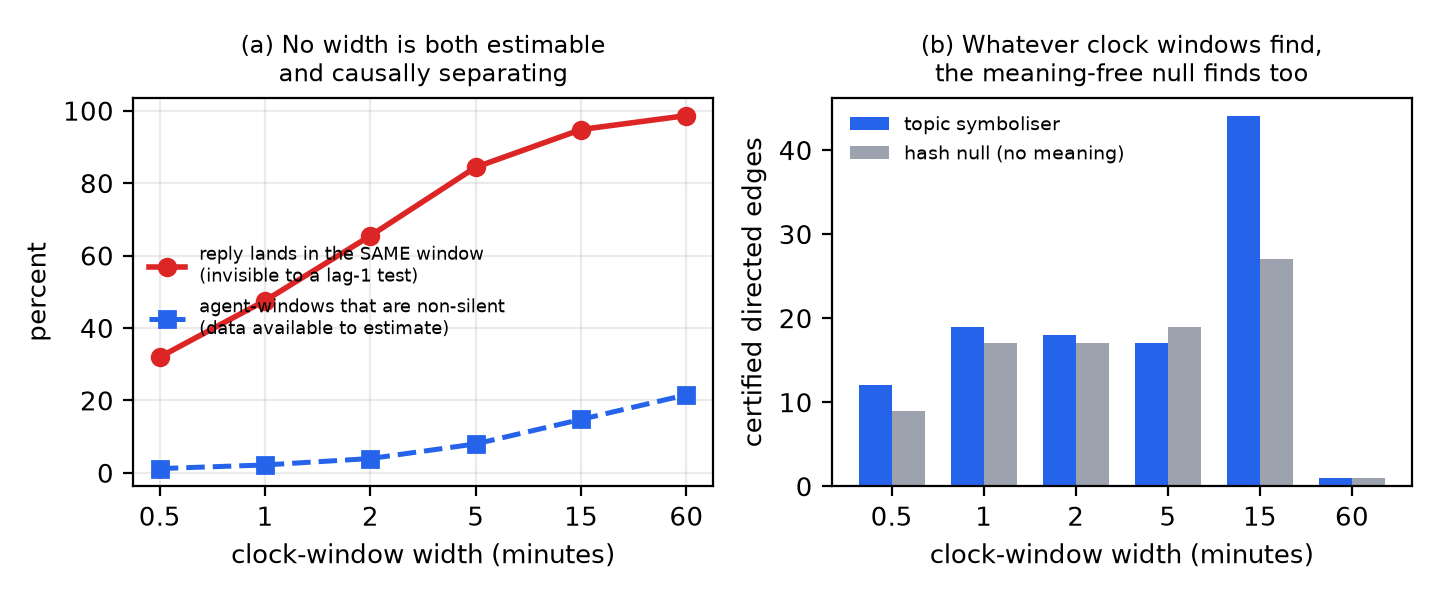
\includegraphics[width=0.92\textwidth]{f1_clock.png}
\caption{Clock-window transfer entropy on the 15 analysed agents of main-village \#general. Left,
the two failure modes as a function of window width. Right, edges certified under the topic
symboliser against the meaning-free hash null.}
\end{figure}

The bind is avoided by ordering messages canonically and letting one message be one tick. Each
agent's series carries its symbol where it spoke and a silent symbol elsewhere, so the lag-1
comparison is between a message and the one immediately before it. The cost is that the measure
captures immediate-predecessor influence only.

\section{The surrogate failure, and two explanations that did not hold}
\label{sec:failure}

An agent is planted into the real stream, drawing its symbols from the channel's marginal and
coupled to nothing at all. It is certified as driving something in 3 of 8 runs when it posts 50
messages, and in 8 of 8 at 100, 263, 600 and 1500 messages, with the mean largest $z$ rising from 5.6
to 12.3, 21.7, 38.3 and 71.7. The error grows with how much the agent speaks, which rules out a
small-sample explanation.

A planted agent could be dismissed as artificial, so the error rate is also measured directly.
Keeping the real speaker sequence and permuting the symbols globally leaves data with no directed
topical influence by construction. The shift surrogate certifies at least one edge in 9 of 10 such
replicates, a family-wise error rate of 0.90 against a nominal 0.05.

\paragraph{What breaks it is the speaker sequence.} Destroying one structure at a time isolates the
cause. Keeping the real speaker order and shuffling only symbols, the shift surrogate fires in 10 of
10 replicates; randomising the speaker order as well drops it to 0 of 10; uniform symbols with the
real order still give 6 of 10. So the driver is the structure of the speaker sequence, not the
symbol distribution and not sparsity. That sequence is far from random in two ways at once: it
repeats a speaker 36\% of the time and returns after one message 38\% of the time, and each agent's
activity is strongly non-stationary, with a median block-share coefficient of variation of 0.79.
Shuffling the order destroys both at once, so this ablation cannot say which of the two mattered.

\subsection{Two explanations I proposed, and the benchmark refuted both}

I initially attributed the failure to mutual exclusivity: only one agent can speak at each tick, so
shifting individual timelines could create overlaps that never occurred in the original
conversation. The benchmark did not support this explanation. A generated channel with exactly one
speaker per tick and steady activity produced an error rate of just 0.025, 95\% Wilson
$[0.011, 0.057]$, far below the 0.90 observed in the real data. Mutual exclusivity alone therefore
cannot explain the failure.

I then suspected turn-taking. In the real channel, speakers repeat 36\% of the time and return after
exactly one message 38\% of the time. However, adding a Markov speaker chain to the generator
produced the opposite result. Turn-taking suppressed the error rather than increasing it. At the
nominal knob values and with no drift the surrogate certified nothing at all across 200 replicates,
while removing turn-taking and introducing drift raised the rate to 0.365. The contribution from
drift was $+0.340$, compared with $-0.025$ for turn-taking. The same inversion appears in the arm
calibrated so that the generated channel reproduces the real channel's measured repeat, return and
block-share statistics rather than merely carrying those numbers as settings: there, turn-taking
alone also certifies nothing, and drift alone gives 0.065.

Neither mechanism, nor their combination in the tested design, reproduced the real-data error rate of
0.90. The largest cell anywhere in the design is 0.365. The real-data ablation removes turn-taking
and non-stationarity together, while the generator separates them. The results point to
non-stationary activity, but the remaining gap means the mechanism behind the full real-data failure
is not yet established.

Every figure above comes from the run at 200 surrogate draws. The first version of this analysis
used 100, which inflates both nulls on the same 2,400 instances: the circular shift fires 53 times
where the 200-draw run does not, against 18 the other way (exact McNemar $p = 3.9 \times 10^{-5}$),
and the permutation surrogate 83 against 20 ($p = 2.7 \times 10^{-10}$). Every qualitative conclusion
in this section is the same at both settings, which is why they are worth stating at all. The
numbers are not, so the draw count belongs in the caption.

\section{The repair, compared}
\label{sec:repair}

Following the local-permutation idea of \citet{runge2018} as adapted by \citet{shorten2021}, each
source keeps its speaking positions and only its symbols are permuted among them. Speaking pattern,
sparsity and turn-taking are preserved exactly, and only the correspondence between symbol and time
is destroyed. On the same destroyed-structure real data the family-wise error rate falls to 0.063
over 300 replicates, 95\% Wilson $[0.041, 0.097]$. The planted uncoupled agent is never certified: 0
of 5 at both 263 and 1500 messages, with mean max $z$ of 2.8 in each case against 22.0 and 68.3
under the shift surrogate.

\begin{figure}[h]
\centering
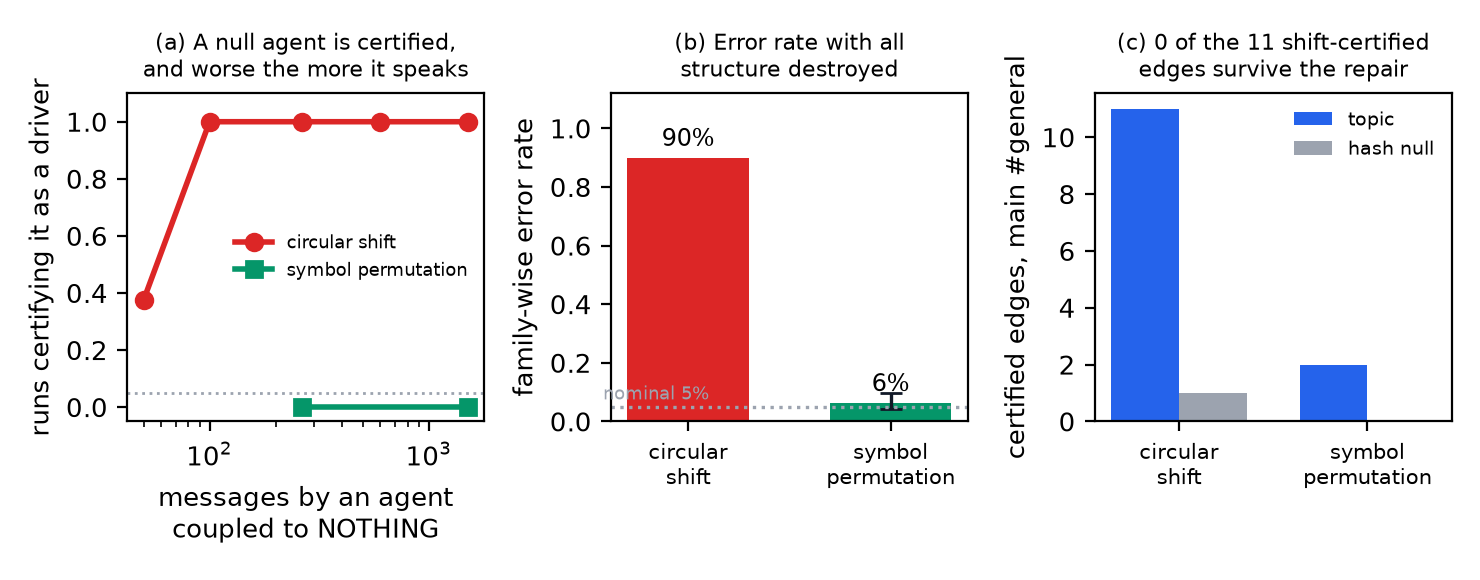
\includegraphics[width=\textwidth]{f2_null.png}
\caption{Left, how often an agent coupled to nothing is certified as a driver, under each surrogate.
Middle, family-wise error rate measured on data with all structure destroyed, with a Wilson
interval; the dotted line is the nominal 0.05. Right, what each surrogate certifies on the real
channel.}
\end{figure}

\subsection{How many surrogate draws are needed}

The number of surrogate draws matters more than I initially appreciated. In a paired comparison of
300 instances, where all four surrogates run on identical symbol grids so the outcomes are paired,
the global permutation surrogate produced a false-positive rate of 0.1167 with 100 draws, falling to
0.0700 with 200 draws, 95\% Wilson $[0.046, 0.105]$. This difference is statistically significant
(exact McNemar $p = 0.0043$). The block-local and Runge local permutations were less sensitive to the
increase: their corresponding rates changed from 0.0900 to 0.0767 and from 0.0967 to 0.0800.

At 200 draws, the global permutation's interval covers the nominal 0.05 and overlaps the real-data
estimate of 0.0633 $[0.0409, 0.0968]$. The real-data result is therefore corroborated rather than
overstated. For practical use, the important point is that reducing the number of surrogate draws
can materially change the result. In particular, the global permutation over-fires at 100 draws by
approximately a factor of two. I would therefore not treat the choice of draw count as a minor
computational detail.

The same correction applies to the benchmark-wide estimate. That figure was 0.0942 at 100 draws.
Repeating all 2,400 instances at 200 draws gives \textbf{0.0679}, 95\% Wilson $[0.0585, 0.0787]$,
and the paired difference is large: 83 instances fire at 100 draws and not at 200, against 20 the
other way, $p = 2.7 \times 10^{-10}$. The conclusion it supports is unchanged, because the interval
still excludes the nominal 0.05. So the permutation repair does carry a residual inflation on clean
generated data, but it is about a third above nominal rather than nearly double.

One limit on this recommendation. I compared 100 draws against 200 and did not test any larger
value, so what the experiment establishes is that 100 is too few, not that 200 is enough. Two
hundred is a lower bound on the draw count rather than a converged setting, and a practitioner whose
conclusions sit near a decision boundary should check their own sensitivity rather than adopt the
number.

\subsection{Choosing a repair, when the error rate cannot choose}

The comparison of the three permutation-based repairs does not produce a clear winner. All four
surrogates were evaluated on identical symbol grids across 300 pure-null replicates, so the
comparison reflects differences between the null models rather than differences between datasets.

\begin{table}[h]
\centering
\begin{tabular}{lrrrl}
\toprule
surrogate & FWER, 100 draws & FWER, 200 draws & 95\% Wilson at 200 & nominal 0.05 \\
\midrule
circular shift                   & 0.0433 & \textbf{0.0333} & $[0.018, 0.060]$ & inside \\
global within-speaker permutation & 0.1167 & \textbf{0.0700} & $[0.046, 0.105]$ & inside \\
block-local permutation          & 0.0900 & \textbf{0.0767} & $[0.052, 0.112]$ & excluded \\
local permutation \citep{runge2018} & 0.0967 & \textbf{0.0800} & $[0.054, 0.116]$ & excluded \\
\bottomrule
\end{tabular}
\caption{Four surrogates on identical symbol grids, 300 pure-null replicates, at both draw counts.}
\end{table}

At 200 draws, paired on the same 300 instances, the circular shift is not significantly different
from the global permutation ($p = 0.0614$), although it differs from block-local permutation
($p = 0.0294$) and from Runge's local permutation ($p = 0.0201$). At 100 draws it differed from all
three, which is the draw-count artifact again. The three repairs remain statistically
indistinguishable from one another, with pairwise $p$-values of 0.85, 0.65 and 1.00. The apparent
differences in their error rates are not sufficient to establish a ranking.

Choosing between them therefore requires more than calibration, and two readings pull against each
other. Runge's local permutation has the strongest methodological justification for preserving the
structure it is intended to preserve, and it follows the approach adapted to event data by
\citet{shorten2021}. Block-local permutation is more heuristic and introduces a free parameter that
has not been tuned. Global permutation is the simplest. On the other hand, the global permutation has
the most favourable interval relative to the nominal rate, and is the only repair that costs nothing
measurable against the shift on clean stationary data, although neither difference is statistically
established. I do not consider the observed error rates sufficient to select one repair over the
others. The choice should be guided by the structure the null is intended to preserve and the
assumptions that can be justified for the data.

\subsection{When to use the repair}

A drift sweep gives the practical reading. Across 150 replicates per cell at 200 surrogate draws,
the circular shift degrades steadily as activity drift increases while the three repairs do not.

\begin{table}[h]
\centering
\begin{tabular}{lrrrr}
\toprule
activity drift & circular shift & global permutation & block-local & local \\
\midrule
0.0 & \textbf{0.013} & 0.093 & 0.080 & 0.093 \\
0.3 & 0.100 & 0.100 & 0.093 & 0.120 \\
0.6 & \textbf{0.193} & 0.053 & 0.047 & 0.067 \\
0.9 & \textbf{0.380} & 0.087 & 0.080 & 0.080 \\
\bottomrule
\end{tabular}
\caption{Family-wise error on pure nulls as activity drift increases, 150 replicates per cell, 200
surrogate draws. Every certified edge is a false positive by construction.}
\end{table}

The pattern is supported by a formal trend test rather than by eye. A Cochran-Armitage test across
the four ordered drift levels gives the circular shift $z = 8.667$, $p < 10^{-15}$, and gives every
repair nothing: $p = 0.51$ for the global permutation, 0.63 for block-local and 0.37 for local. The
same pattern holds at both surrogate draw counts, so it does not depend on that choice.

The repairs are therefore flat under drift rather than calibrated. Only one of the four global
permutation intervals covers the nominal 0.05, and the rest sit nearer 0.09, so what the repair buys
is insensitivity to drift rather than correctness. One asymmetry should be stated rather than
hidden: block-local covers nominal in three of the four cells where the global repair covers one.
The two remain pairwise indistinguishable, so this is not grounds to switch the recommendation, but
it does mean the global repair cannot be described as the best-calibrated under drift.

The results also show why the repair should not be treated as universally preferable. At zero drift
the circular shift has an error rate of 0.013, while the three repairs are all around 0.08 to 0.09.
That advantage is gone by the first drift step: at drift 0.3 the shift reads 0.100 against the global
permutation's 0.100 and block-local's 0.093, so the crossover falls between drift 0.0 and 0.3 rather
than at some higher level. By drift 0.6 the shift is roughly four times the repairs. If a channel has
been checked and found stationary, the circular shift may be sufficient. When activity is
non-stationary the repairs are the more stable choice, and the margin for error on that judgement is
narrow, because the crossover arrives by the first drift level tested.

\section{Continuous time, and what the repair cannot test}

An earlier analysis identified continuous-time estimation as the principled option for event data
but did not evaluate it. Running the continuous-time estimator CoTETE on both channels certifies 0
edges in either case, compared with 2 for main-village and 18 for open-chat under the discrete,
turn-ordered analysis. Its highest $z$-scores are 3.062 and 3.980, below the respective max-T
thresholds of 4.171 and 4.308.

At first these results might appear to contradict the symbol-based analysis. The two estimators
operate on different information, however. CoTETE's public API takes event times with no symbol
channel, while the transfer-entropy analysis here uses topic symbols. To test whether this
difference explains the results, I reduced the data to timing alone, replacing every spoken symbol
with the same code. Under this representation the estimator used here also detects 0 edges in both
channels, matching CoTETE. Using the circular-shift surrogate instead produces 12 and 3 edges. So
neither method detects relationships from event timing alone in these channels, and the edges found
by the symbol-based analysis depend on symbol correspondence, which the continuous-time estimator
cannot access.

Two caveats attach to those $z$-scores, and the second attaches to the larger of them. Point
estimates from this estimator are stochastic to about 17\% across repeated runs, so none of these
values should be read to more than two significant figures. And open-chat's highest $z$, the 3.980,
belongs to the one pair whose surrogate draws mostly failed: it needed 1,936 failed draws to obtain
100 successes, a 4.9\% success rate. Those surrogates are conditioned on being estimable, so that
pair's null is biased in an unknown direction. The conclusion does not rest on it, since that pair
falls below threshold and so does every other pair, but the number should not be quoted as a clean
measurement. The failures themselves were a defect rather than a property of the data: an enlarged
exclusion window can empty the neighbour search on sparse bursty event trains and raise an error
that terminates a whole pair, with no handling at the public entry point. This has been reported
upstream.

There is also a fundamental limitation in applying the recommended permutation surrogate to
timing-only data. When every event carries the same symbol, permuting those symbols changes nothing.
The observed statistic and the surrogate null are identical, making the test exactly degenerate:
standard deviation 0 across all 210 pairs and $p = 1.0$ everywhere. \textbf{The repair has zero power
against timing structure by construction.} The permutation surrogate is appropriate for testing
relationships in the symbol sequence, but it does not answer whether relationships exist in event
timing. These are different questions, and choosing one null means giving up the ability to test the
other with that procedure.

\section{Confounding, and what conditioning removes}

A valid surrogate fixes calibration but not confounding. If every agent tracks a drifting channel
topic, every pair is genuinely dependent through the channel, and pairwise transfer entropy cannot
tell that from direct influence. I therefore also report a \textbf{conditional} estimate, which asks
whether a source's last message adds anything about a target's next one beyond the target's own
history and the channel's recent state. The conditioning variable is the modal symbol of the last
twelve messages, excluding the immediately preceding one so that it does not simply restate the
source.

On a generated benchmark whose decisive instances contain no influence while every agent tracks a
shared drifting topic, so that any certified edge is common cause, pairwise transfer entropy
certifies \textbf{22.3} edges on average and conditioning takes that to \textbf{0.33}, lifting pooled
precision on the four-edge instances from 0.17 to \textbf{0.80} at a recall of 1.0 either way. Across
couplings from 0.05 to 0.8 the conditional test still finds the planted edge in 3 of 3 runs, so the
gain costs no power.

The benchmark flatters the conditional estimator, since its common cause is a shared modal topic and
the conditioning variable is the channel's modal topic. The real channels are harder, and
conditioning there costs degrees of freedom: a 9-symbol alphabet with a 9-valued context gives 6,561
cells against about 7,900 ticks, so that variable is also coarsened to 4 and 2 values.

\begin{table}[h]
\centering
\begin{tabular}{lrrrr}
\toprule
channel & pairwise & conditional, 9 values & 4 values & 2 values \\
\midrule
main \#general      & 2  & \textbf{2, the same two edges} & 2 & 3 \\
open-chat \#general & 18 & \textbf{0} & \textbf{7} & \textbf{13} \\
swarm, room a       & 1  & \textbf{0} & & \\
\bottomrule
\end{tabular}
\caption{Conditioning at three resolutions. Main-village's two edges are robust to that choice;
open-chat's zero is not.}
\end{table}

At the finest resolution the open-chat test is degenerate, its surrogate sitting above the observed
statistic for 65\% of pairs with the largest $z$ in the family only 4.4, so it is failing to reject
rather than finding nothing to reject. Open-chat's structure therefore remains
\textbf{undetermined}: depending on the conditioning resolution, between 0 and 13 of its 18 edges may
survive. That resolution is a free parameter an analyst would set once and never revisit. This is a
property of the channel rather than the estimator: on structure-free real data the conditional test
fires in 2 of 40 replicates, an error rate of 0.05 with a mean $z$ of $-0.001$, so it is nominal
rather than conservative.

\section{The symbolisation floor}
\label{sec:floor}

Everything these methods produce is downstream of turning text into symbols. On the benchmark, where
the underlying topics are known, detection performance drops sharply when agreement between the
symboliser and the ground truth falls below roughly ARI 0.44, and this behaviour appears across the
tested estimators. Importantly, the false-positive rate can look \emph{better} below this point,
because the shared topic structure needed to produce confounded detections is no longer represented
reliably. A pipeline that stops detecting relationships may therefore have lost the signal it needs
rather than become more reliable, and nothing downstream of the symboliser can tell those apart.

\subsection{Detecting the floor without labels}

That degradation can be detected without ground-truth labels. Across the nine-level benchmark sweep,
three statistics separate the below-floor cases with zero errors: seed stability at a threshold of
0.623, agreement with LSA at 0.646, and the Calinski-Harabasz index at 138.9. Seed stability here is
the \textbf{minimum} pairwise agreement across seeds, not the mean; the mean variant makes one error,
at a different threshold of 0.791. Silhouette has the strongest correlation with true ARI, at 0.979,
but is not useful for identifying the boundary because its threshold falls within a gap of just
0.002. A statistic that tracks clustering quality most closely is not necessarily the best one for
making a classification decision.

Error count cannot choose among the three that were perfect, so I tested whether each threshold still
means what it meant when the channel changes for reasons other than topic separability. Applying each
cut unchanged to thirty cells that vary turn-taking, drift, agent count, volume skew, message length
and corpus size, twenty-seven of which hold true ARI at exactly 1.000:

\begin{table}[h]
\centering
\begin{tabular}{lrrrr}
\toprule
diagnostic & cut & errors where fitted & errors, nuisance set & of those at true ARI 1.000 \\
\midrule
seed stability, min across seeds & 0.623 & 0 & 2 & \textbf{0} \\
LSA agreement                    & 0.646 & 0 & 2 & \textbf{0} \\
Calinski-Harabasz                & 138.9 & 0 & 6 & \textbf{3} \\
\bottomrule
\end{tabular}
\caption{Whether a cut fitted on the vocabulary-overlap mechanism survives a change in the channel
that is not a change in topic separability.}
\end{table}

The two bounded statistics err only on the short-message cells, where the symbolisation genuinely has
degraded. Calinski-Harabasz additionally condemns all three cells whose true ARI is exactly 1.000,
for no reason beyond the corpus holding 2,000 messages rather than 8,000, where it reads 76 to 77
against its own cut of 138.9. It is unbounded and grows with sample size, so a published numeric
threshold for it carries no meaning on another corpus. That is why I recommend the two bounded
statistics and not the index that matched them on error count. \textbf{A cut that moves with the
corpus is not a floor cut.}

This is not a weak statistic being discarded on a technicality. Calinski-Harabasz correlates with
true ARI at 0.973, almost as closely as silhouette, and unlike silhouette it classifies the floor
perfectly where it was fitted. It still cannot carry a published threshold. That is the sharper form
of the point above: neither the statistic that tracks quality most closely nor the one that
classifies best on the fitting mechanism is necessarily the one whose cut another researcher can
reuse.

There are important limits to this result. The effective sample size is nine rather than 54, because
the classification label is determined by overlap level. There are no observations between ARI 0.444
and 0.222, so the exact location of the boundary within that interval remains unknown. These
diagnostics classify whether a result is below the tested detection floor; they do not estimate ARI,
and their behaviour is flat between 0.68 and 1.00, and not even monotone there. The benchmark also
uses a single degradation mechanism with a known and correct value of $k$, whereas the true number of
topics in real conversations is unknown. I therefore treat 0.44 as a benchmark-specific, bracketed
result rather than a universal threshold.

\subsection{A contradiction the diagnostic lost}

I initially used these diagnostics to classify one real channel, open-chat, as below the
symbolisation floor. That conclusion did not agree with the channel's measured results: open-chat
certified 18 and 22 edges under the two symbolisers, compared with 2 and 1 for main-village, and its
hash-based null certified zero edges. Rather than treating this disagreement as evidence that the
original measurements were wrong, I revisited the diagnostic itself.

The problem was the choice of $k$. Repeating the comparison with the same channels, loader and window
reproduced the published $k=8$ results to the digit. At $k=4$, however, open-chat reached stability
scores of 0.950 and 0.978, the highest values produced by either channel across the tested settings,
and both exceeded the diagnostic thresholds. The earlier below-floor classification was therefore a
conclusion about one arbitrary choice of $k$, not a reliable statement about the channel. Message
length does not explain the difference either: 27.1\% of main-village messages contain fewer than
five tokens, compared with 2.3\% in open-chat, so the short-message channel is the one the diagnostic
cleared.

This correction changes how the symbolisation results should be read, and it withdrew three claims.

\begin{enumerate}
\item \textbf{The claim that no topic signal remains below the floor is too strong.} The
circular-shift surrogate recovers all four planted edges at every tested overlap level, including
0.95, where ARI is 0.011. The observed collapse is in the permutation null, not necessarily in the
underlying data.
\item \textbf{ARI 0.44 cannot be treated as a universal detection threshold.} When the shared-topic
parameter is 0, detection continues down to ARI 0.296, so the boundary depends on both the
symboliser and the channel.
\item \textbf{Edge counts cannot be used as a measure of symboliser quality.} Even at ARI exactly
1.000, changing the shared-topic parameter alone moves the permutation edge count from 5 to 78.
\end{enumerate}

The diagnostics also do not transfer reliably outside the mechanism on which they were evaluated.
Their balanced accuracy falls from 1.00 to 0.75 and 0.571 under a known mismatch in $k$. All seven
errors made by seed stability are false below-floor classifications, and in every one of those cases
the detector still identifies all planted edges; of the fourteen cells it condemned, eleven had full
conditional recall. The failure direction is the dangerous one: it condemns working symbolisations.

This was an important correction to my own interpretation. I introduced a diagnostic to check whether
the symbolisation was reliable, applied it to the real channels, and found that it contradicted
measurements already in hand. Investigating that contradiction showed the diagnostic was sensitive to
an arbitrary modelling choice. The result is not that the original measurements were wrong, but that
the control was being asked to support a broader conclusion than the evidence allowed. These
diagnostics remain useful within their tested setting, and \textbf{no channel-level floor verdict
should be issued from a single $k$}.

\section{The benchmark}

Real logs have no ground truth, so the common-cause question could not be settled on them. The
generator used here makes the influence graph known by construction: it decides, in code, who speaks
at which tick, on which topic, and who reacts to whom. Surface text is a separate, replaceable layer
drawn from disjoint per-topic vocabularies, so the whole thing runs offline and a detector still has
to symbolise raw text rather than read the labels. Turn-taking and activity drift are independent
knobs, so the two can be varied one at a time, and the generator reproduces its earlier behaviour
bit for bit when both are zero.

\benchname{} is released with 150 tests covering the generator, the detector harness, the text layer,
the floor analysis and the turn-taking factorial.
\ifdeanon{Code and benchmark:
\url{https://github.com/manunicholasjacob/swarm-influence-bench} and
\url{https://github.com/manunicholasjacob/swarm-influence-audit}.}{Code and benchmark are publicly
released; the links are withheld here for anonymity and will be given in the camera-ready version.}

One property of the benchmark must be stated when its numbers are quoted. Planting an edge displaces
other agents' speaking turns, so the generated instances contain real lag-1 dependencies that the
label set does not list. Precision measured against those labels is therefore a \textbf{lower bound}
for any detector, and what the benchmark supports is the comparison between two estimators rather
than the absolute value of either.

\section{What an overseer should do}

Six inexpensive controls should be included whenever an influence graph over an agent channel is
published.

\begin{enumerate}
\item \textbf{Plant an agent coupled to nothing, at your channel's volumes, and check it is not
certified.} This one test would have caught the failure reported here, at one run per volume.
\item \textbf{Measure the error rate directly}, by destroying the structure your method claims to
find and checking the family-wise rate is near nominal. If it is not, your surrogate does not match
your data.
\item \textbf{Preserve the speaker sequence in your surrogate.} Any surrogate that moves an agent's
messages in time will disturb it, and \citet{shorten2021} is the principled route. Use at least 200
surrogate draws, because at 100 the global within-speaker permutation over-fires by roughly a factor
of two.
\item \textbf{Establish the detection floor before interpreting an absence.} ``No edges'' and ``no
influence'' are different claims.
\item \textbf{Condition on the channel, report both numbers, and sweep the resolution.} Pairwise and
conditional bound the answer, and the gap between them is the result. Conditioning costs cells, so
check whether your answer is an artifact of how finely you conditioned. On one channel here it was.
\item \textbf{Report how well your symboliser agrees with the truth, on data where you know it.}
Everything is downstream of turning text into symbols, and below roughly ARI 0.44 detection
collapses whatever the estimator. I have found this control in no influence-detection paper, and it
is also the one that cannot be run on real logs, which is why the floor remains the largest
unquantified threat here.
\end{enumerate}

Two habits follow: publish a meaning-free null's count beside the real one, and require held-out
replication before calling a graph a structure.

\section{The real channels, and what survives}

Re-running every channel under the repaired surrogate changes the answers, and not in one direction.

\begin{table}[h]
\centering
\begin{tabular}{lrrr}
\toprule
channel & window messages & shift: topic / hash & permutation: topic / hash \\
\midrule
main \#general      & 8,800 & 11 / 1 & 2 / 0 \\
open-chat \#general & 8,226 & 3 / 0  & 18 / 0 \\
swarm, room a       & 3,846 & 2 / 1  & 1 / 0 \\
\bottomrule
\end{tabular}
\caption{The same channels under both surrogates, with the meaning-free hash null beside each.}
\end{table}

In main-village, \textbf{none} of the 11 edges the standard recipe certifies survives the repair, and
the two the valid surrogate certifies were not among them. In open-chat the correction runs the other
way, 3 edges becoming 18, because pathological pairs inflate the max-T threshold and raise the bar
for everything else. An invalid surrogate does not simply add false positives; it scrambles the
result.

Main-village's two edges are the strongest thing here and they are still not a finding, because they
do not replicate: the adjacent fourteen-day window certifies nothing at all under either estimator.
Given the detection floor, that silence is as consistent with the test sitting near its limit as with
the edges being absent, and the two cannot be separated. Power is governed by how much an agent says
as much as by how strongly it copies, and it is channel-specific: in main-village a planted follower
copying on 80\% of its messages is caught only 1 time in 4, while in open-chat one copying 10\% of
the time is caught 3 times in 4. Replication is weak everywhere: under the standard recipe the
adjacent window shares 1 edge out of 8 and 4, and that edge is also the only one the hash null
certifies. No certified edge in this work replicates out of sample.

\begin{figure}[h]
\centering
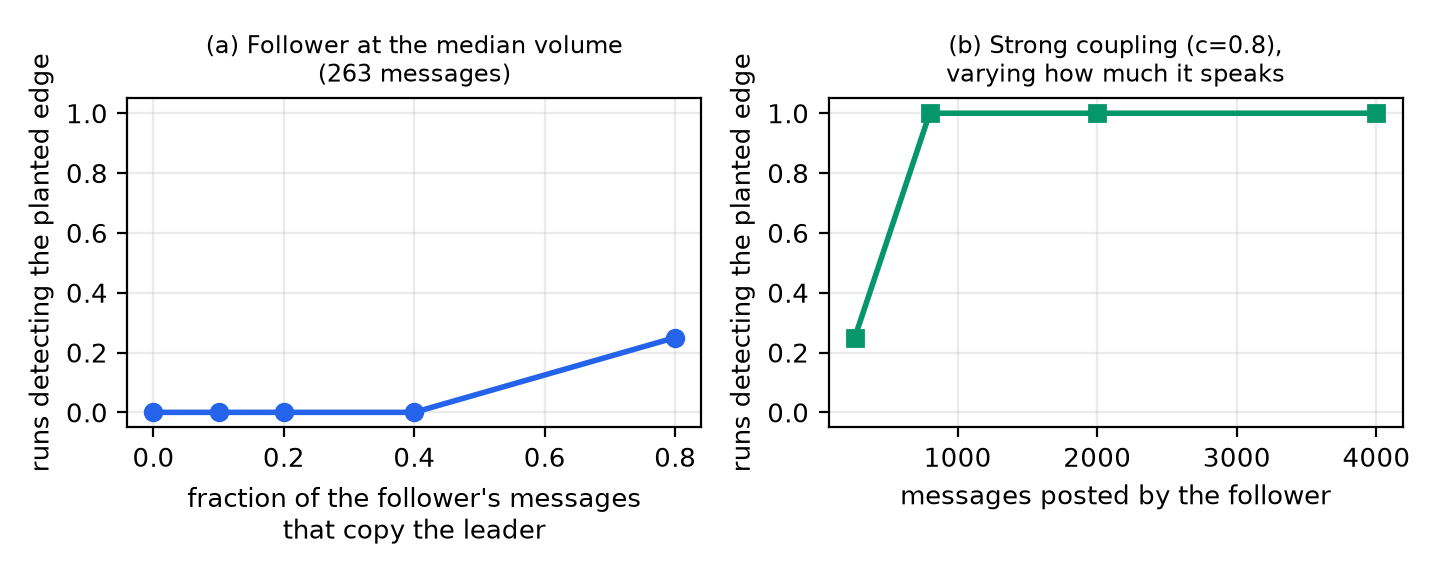
\includegraphics[width=0.92\textwidth]{f4_power.png}
\caption{Detection of a planted follower under the repaired surrogate. Left, varying the fraction of
its messages that copy the leader, at the median agent's volume. Right, varying how much it speaks,
at strong coupling.}
\end{figure}

\paragraph{Humans in the channel.} Main-village \#general is now effectively human-free, with 3 human
messages in the window, so the question has to be asked in open-chat, where 32\% of messages come
from 124 human visitors. Pairwise, with humans collapsed into one node, 19 edges are certified.
Conditioning removes almost all the agent-to-agent structure and little of the rest: \textbf{four
edges survive, of which three run from humans to agents, one is agent to agent, and none run from an
agent to a human.} The asymmetry is not an artifact of the confound. It should be read carefully all
the same: topical dependence from a person to an agent is also what ordinary responsiveness looks
like, so the measurement supports only that the dependence is dyad-specific and directional, not
that anyone is steering a swarm.

\section{Reproducibility, and one limitation of it}

Every number in this paper is recomputed from committed analysis output by a verifier that fails on a
mismatch, and that verifier covers the prose of this paper as well as the figures.

One limitation should be stated plainly. Re-running the counts in the earlier stationarity sweep with
the same seeds and configuration, only one of the eight cells reproduced exactly; the remaining
differences were one or two replicates per cell. Seven of the eight published rates still fell within
the recomputed Wilson intervals, and no conclusion changed. The exception is the zero-drift cell under
the permutation null, where the published 1 of 30 falls just below the recomputed interval of
$[0.035, 0.256]$ for 3 of 30, and no result here depends on that cell.

The generator, estimator and BLAS configuration were investigated and ruled out as the source. The
most likely explanation is a library-level difference, particularly in scikit-learn's $k$-means
implementation within the symboliser, whose output can vary between versions. Every sweep now records
the environment it ran under: Python 3.14.6, numpy 2.5.1, scipy 1.18.0 and scikit-learn 1.9.0,
including the BLAS build and the number of BLAS threads each worker used.

This does not make the previously published counts exactly reproducible. It provides a more clearly
specified environment in which subsequent results can be checked. For that reason I report rates
alongside their confidence intervals rather than exact replicate counts. The distinction between
reproducing a result within its uncertainty and reproducing every individual count matters, and only
the first is claimed.

\section{Conclusion}

Applied to real agent chat, the standard recipe for ``who drives whom'' needs repair before it says
anything. Clock windows cannot separate a message from its answer at the speed agents reply, and what
they certify is matched by a null with no access to meaning. The turn-ordered grid that fixes this
breaks the circular-shift surrogate: family-wise error 0.90 against a nominal 0.05, caused by the
speaker sequence itself. Restricted permutation surrogates repair most of that, but they are flat
under drift rather than calibrated, they are mutually indistinguishable at this precision, and one of
them needs twice the surrogate draws anyone would think to use. A valid surrogate fixes calibration
but not confounding. What survives is small: two dyad-specific edges that do not replicate, an
undetermined answer set by conditioning resolution, and influence running from people into agents and
never back. \textbf{An influence graph should not guide decisions until its error rate, its confound,
its detection floor and its symboliser's fidelity are reported.}

\section*{Limitations}

\begin{itemize}
\item \textbf{Immediate-predecessor only.} The turn-ordered lag-1 measure sees influence from the
message directly before a reply. Influence acting over several turns, or through a room's accumulated
context, is out of scope.
\item \textbf{Discrete approximation to an event process.} Agent chat is event-based in continuous
time. The turn-ordered discretisation with a permutation surrogate is a practical fix, and the
continuous-time comparison above shows what that choice gives up.
\item \textbf{The mechanism behind the real 0.90 is not established.} The generator separates
turn-taking from drift and points at drift, but the largest cell anywhere in the design is 0.365.
\item \textbf{Symbolisation quality cannot be measured on the real logs.} The central result survives
an independent symboliser, but the edge count does not: it moves with alphabet size and with which
messages the topic model is fit on. The floor remains the largest unquantified threat.
\item \textbf{No ground truth in the real logs.} The validity argument rests on planted controls and
on the meaning-free null, not on recovering a known answer.
\item \textbf{Conditioning removes real influence too.} The conditional estimate discards influence
that works by shifting what the channel is talking about, which in a group chat may be a large part
of genuine influence. It is a lower bound on dyadic influence.
\item \textbf{The human result is exploratory.} It rests on one village and one window and should be
read as a lead.
\end{itemize}

\section*{Broader impact and ethics}

This work audits influence detection on a population of AI agents, which is dual-use. Used
defensively it helps an overseer decide what an influence graph is worth, and the main result is
deflationary: it tells practitioners to trust these outputs less, which reduces rather than increases
the chance of acting on a bad attribution. The same tooling could be used to identify the most
influential agent in a swarm in order to target it, or to surveil participants in a channel. Three
properties limit the misuse. The subjects are AI models; the dataset is already public under research
terms and no re-identification is added; and the measure is weak and local, recovering
immediate-predecessor topical dependence rather than any model of how to steer an agent.

The dataset's research terms were followed: research use only, no training on the data, no
re-identification, citation of the source, and notification of the authors of resulting publications.
Human participants appear only as an aggregate node or as anonymised visitor labels, never by name or
handle, and no content attributable to an individual person is reported. Message text and metadata
were read, never model weights or private user data.

The use of a large language model in this work is disclosed in the first-page footnote, as TMLR
requires.

\bibliographystyle{tmlr}
\bibliography{refs}

\end{document}
"               camera-ready
% Use build.py, which runs all of them and checks the anonymous output for leaks.
\providecommand{\TMLRMODE}{submission}
\makeatletter
\def\@tmlrpreprint{preprint}
\def\@tmlraccepted{accepted}
\ifx\TMLRMODE\@tmlrpreprint
  \usepackage[preprint]{tmlr}
\else
  \ifx\TMLRMODE\@tmlraccepted
    \usepackage[accepted]{tmlr}
  \else
    \usepackage{tmlr}
  \fi
\fi
\makeatother

\usepackage{hyperref}
\usepackage{url}
\usepackage{booktabs}
\usepackage{graphicx}
\usepackage{amsmath}

% Gate every identifying string on whether identity may be revealed at all. The flag to test is
% \if@accepted, NOT \if@preprint: tmlr.sty's [preprint] option sets BOTH, so \if@accepted is true
% for the preprint and the camera-ready and false only for the anonymous submission, which is
% exactly the condition wanted. Gating on \if@preprint alone also hid the repository URLs from the
% camera-ready, which is where this paper promises to give them. \if@accepted is internal to
% tmlr.sty, hence the \makeatletter. The anonymous build takes the second argument.
\makeatletter
\newcommand{\ifdeanon}[2]{\if@accepted#1\else#2\fi}
\makeatother
\newcommand{\benchname}{\ifdeanon{SwarmInfluence-Bench}{the benchmark}}

% An unmarked footnote, for the LLM-use disclosure. TMLR's FAQ requires the disclosure and names
% the location: authors must "mention explicitly in their submission that they have used this
% tool", "as a footnote on the first page". Verified against jmlr.org/tmlr/faq.html on 10 Nov 2026.
% It is therefore not optional, and it does not belong in Broader Impact, where it sat until now.
% Nothing in the policy asks for the vendor's name, so none is given.
\newcommand{\disclosurefootnote}[1]{%
  \begingroup\renewcommand\thefootnote{}\footnote{#1}\addtocounter{footnote}{-1}\endgroup}

\title{An Influence Graph Over AI Agents Certifies an Agent That Copies Nobody}

% Hidden by the tmlr package unless [accepted] or [preprint] is given.
\author{\name Manu Nicholas Jacob \email manunicholasjacob@gmail.com \\
        \addr Independent Researcher}

\def\month{11}
\def\year{2026}
\def\openreview{\url{https://openreview.net/forum?id=XXXXXXXXXX}}

\begin{document}
\maketitle

\begin{abstract}
Circular-shift surrogates can produce severely inflated false-positive rates when applied to
turn-ordered multi-agent conversations, reaching a family-wise error rate of 0.90 against a nominal
0.05. A generated benchmark separates two candidate mechanisms and points at non-stationary speaker
activity rather than turn-taking, which suppresses the failure rather than causing it. No setting of
either knob reproduces the observed 0.90, however, so what drives the full real-data failure remains
open. Restricted permutation surrogates substantially reduce the problem. Their error rate is flat
with respect to drift rather than at the nominal level, and for the global within-speaker variant it
depends on how many surrogate draws the null is built from. Calibration alone does not address
confounding, which motivates a conditional estimator validated against a benchmark with planted
ground truth. I also identify a symbolisation-dependent detection limit and develop label-free
diagnostics for it, and show that their calibration does not transport across degradation
mechanisms. The benchmark is released.
\end{abstract}

\disclosurefootnote{\textbf{Use of a large language model.} A large language model was used as an
assistive tool: to help write and run the analysis code, and to help draft this paper. The author is
responsible for every claim, number and figure. All results come from the released code run on the
public dataset, no result or reference is fabricated, and every number in this paper is recomputed
from committed analysis output by a verifier that fails the build on a mismatch.}

\section{Introduction}

When AI agents interact in a shared channel, it is useful to understand how they influence one
another. Information-theoretic methods offer a way to measure this through lagged transfer entropy,
surrogate testing, and per-agent influence scores. They are attractive because they require no
labels and no access to model internals, only a record of who said what and when. The reliability of
those measurements is what this paper examines.

Almost every demonstration of these detectors runs on synthetic traces with a planted leader, where
the analyst controls timing and vocabulary. Real agent chat is asynchronous, bursty, and written in
open language. The narrower question here is whether the standard recipe, applied to real agent
logs, returns anything an overseer should act on.

The audit runs on the AI Village corpus \citep{aidigest2026}, in which frontier models share chat
channels over eighteen months across four villages differing in size, lifetime and tempo, applying
the checks a reader should demand: planted controls, a meaning-free symboliser, replication in a
held-out window, and sensitivity to every parameter that had to be chosen.

\begin{enumerate}
\item The conventional circular-shift surrogate is \textbf{invalid} on turn-ordered agent chat: a
family-wise error rate of 0.90 against a nominal 0.05, caused by the structure of the speaker
sequence itself.
\item Restricted permutation surrogates restore most of the calibration, and re-certifying under one
\textbf{scrambles rather than shrinks} the answer: one channel loses all 11 of its edges, another
gains 15.
\item The three restricted variants are \textbf{mutually indistinguishable} at the precision reached
here, so the choice between them cannot be justified on error rate. The global within-speaker
variant additionally needs on the order of 200 surrogate draws, and over-fires by roughly a factor
of two at 100.
\item Calibration is not confounding, so a conditional estimate is added and validated on a released
benchmark with a known influence graph: common-cause false edges fall from 22.3 to 0.33, and on the
planted-edge instances precision rises from 0.17 to 0.80 with no loss of recall or power.
\item The same benchmark exposes a \textbf{symbolisation floor}. Below roughly 0.44 adjusted Rand
index between symboliser and truth, detection collapses whatever the estimator. Label-free
diagnostics detect that floor, but their calibration does not transport across degradation
mechanisms, and I report where it fails.
\item On the real channels two edges stand at every conditioning resolution, 18 are
\textbf{undetermined} between 0 and 13, none replicates out of sample, and what survives alongside
humans runs from people to agents.
\end{enumerate}

\section{Related work}

\paragraph{Transfer entropy and surrogates.} Transfer entropy \citep{schreiber2000} measures how much
a source's past reduces uncertainty about a target's next symbol beyond the target's own past.
Plug-in estimators are biased upward on short series, so significance rests on surrogate data, with
family-wise error controlled by a max-T test \citep{westfall1993}. The usual surrogate is a circular
time shift of the source.

\paragraph{Event-based data breaks the shift surrogate.} \citet{shorten2021}, on neural spike trains,
show that the conventional source-time-shift surrogate fails to represent the null hypothesis of
conditional independence for event-based processes, and adapt to that setting the nearest-neighbour
local permutation scheme of \citet{runge2018}. Agent chat is event-based in that sense: messages are
events in continuous time, not samples of a clocked signal. The correction is not a contribution of
this paper. The contribution is showing that the same failure carries over to multi-agent safety
monitoring, and that it can be severe enough to create apparent leaders where none exist.

\paragraph{The same failure, concurrently, in multi-agent reinforcement learning.}
\citet{papadopoulos2026} report a closely related surrogate failure in multi-agent
reinforcement-learning action series. Their agent pairs have zero influence by construction, yet
circular time shifts produce false-positive rates of 100\% and 98.2\% against a nominal 0.05. A
plain permutation surrogate fares no better in their setting, at 100.00\% and 99.95\%. Their
proposed correction restricts permutations to blocks of training time, which returns the rates to
5.25\% and 5.50\%.

There are important differences between their setting and this one. Their data consist of binary
actions recorded over twelve thousand training rounds, whereas these data are symbolised
natural-language messages arranged on a turn-ordered conversational grid. Their non-stationarity
comes from monotone drift associated with annealing exploration; here the relevant non-stationarity
appears in the speaker sequence. Neither result should be taken as a direct extension of the other.

Nevertheless, the fact that both approaches rely on restricted permutations is worth noting. Their
permutation blocks are defined by training time, while mine are defined by an agent's own speaking
positions. This provides convergent evidence that unrestricted temporal rearrangement can be
problematic in non-stationary multi-agent data. Their findings also serve as a useful warning for
the approach taken here, and the warning has a measured form rather than a rhetorical one: in their
data the unrestricted permutation failed as completely as the time shift, at 100.00\% against a
nominal 0.05. Permutation-based surrogates are not automatically protected against
non-stationarity, and what protects the one used here is the restriction, not the permutation. I
claim no priority over their result and view the two studies as complementary, addressing different
forms of structured multi-agent data.

\paragraph{Oversight under a budget.} AI-control research frames monitoring as resource constrained,
with a cost for false positives \citep{greenblatt2024}. An influence graph is one such measurement,
and its error rate is the concern here.

\paragraph{Clustering stability.} The idea of using clustering stability as a label-free quality
indicator is not new. It has a substantial history, including \citet{benhur2002},
\citet{lange2004}, von Luxburg's review of clustering stability \citep{vonluxburg2010}, and
\citet{tibshirani2005} on prediction strength. What is different in Section~\ref{sec:floor} is the
calibration of these diagnostics against a detection-performance floor rather than against cluster
recovery alone.

\section{Data and representation}

The AI Village dataset ships one gzipped-JSONL table per village. Four villages are used, differing
enough to test whether any finding is a property of one channel.

\begin{table}[h]
\centering
\begin{tabular}{lrrrrl}
\toprule
village & agent messages & agents & lifetime & human messages & busiest room \\
\midrule
main      & 205,726 & 58  & 576 days & 10,029 & \#general (166,715, 81\%) \\
open-chat &  35,483 & 23  &  66 days & 12,264 & \#general (all) \\
swarm     &   3,848 & 133 &   1 day  &      5 & room a (3,846) \\
game-jam  &     838 & 6   &   3 days &     36 & per-team rooms \\
\bottomrule
\end{tabular}
\caption{The four villages. A 2026 scaffolding change scopes each agent to its current room's
context, so the busiest room of each village is a self-contained influence substrate and is analysed
alone.}
\end{table}

The primary window is the final fourteen days of main-village \#general, 17 to 31 October 2026,
holding 8,800 agent messages. Twenty-two models posted at least 50 messages each and the directed
test uses the 15 busiest, giving 7,958 message events. Two scaffolding facts are disclosed rather
than corrected: the automated nudger was off throughout, and the unused \#best and \#rest rooms were
soft-deleted mid-window, which does not touch \#general.

\subsection{From open language to symbols}

Transfer entropy needs discrete symbols, so each message is mapped to a small alphabet before
influence is estimated, and that mapping is kept separate from the estimator. A topic symboliser
(TF-IDF then $k$-means, $k=8$) gives a message its topic cluster id, so paraphrases of one idea share
a symbol. A hash symboliser, a stable hash of the normalised text into $k=8$ buckets, has no notion
of meaning and serves as a null: an edge appearing under both lives in timing alone.

\subsection{The lag problem, and why clock windows cannot solve it}

A lag-1 transfer entropy compares window $t-1$ with window $t$, so influence landing inside one
window is invisible to it. Agent chat makes this binding. Among the fifteen analysed agents the gap
between consecutive messages by different speakers has a median of 28.1 seconds (25th percentile
9.2, 75th 66.2, 95th 159.3), so turn-taking is a seconds-scale process while any clock window wide
enough to hold two speakers is minutes wide and swallows both a message and its answer.

Both horns are measurable. At 30 seconds only 1.2\% of agent-windows hold a message, while 32.0\% of
replies already land in the same window as what they answer, rising to 84.4\% at five minutes. At
every width tried, the meaning-free hash null certifies comparably many edges, and more at five
minutes: 9 against 12 at thirty seconds, 17 against 19 at one minute, 27 against 44 at fifteen, and
19 against 17 at five. Whatever clock-window transfer entropy was detecting there, it was not shared
meaning.

\begin{figure}[h]
\centering
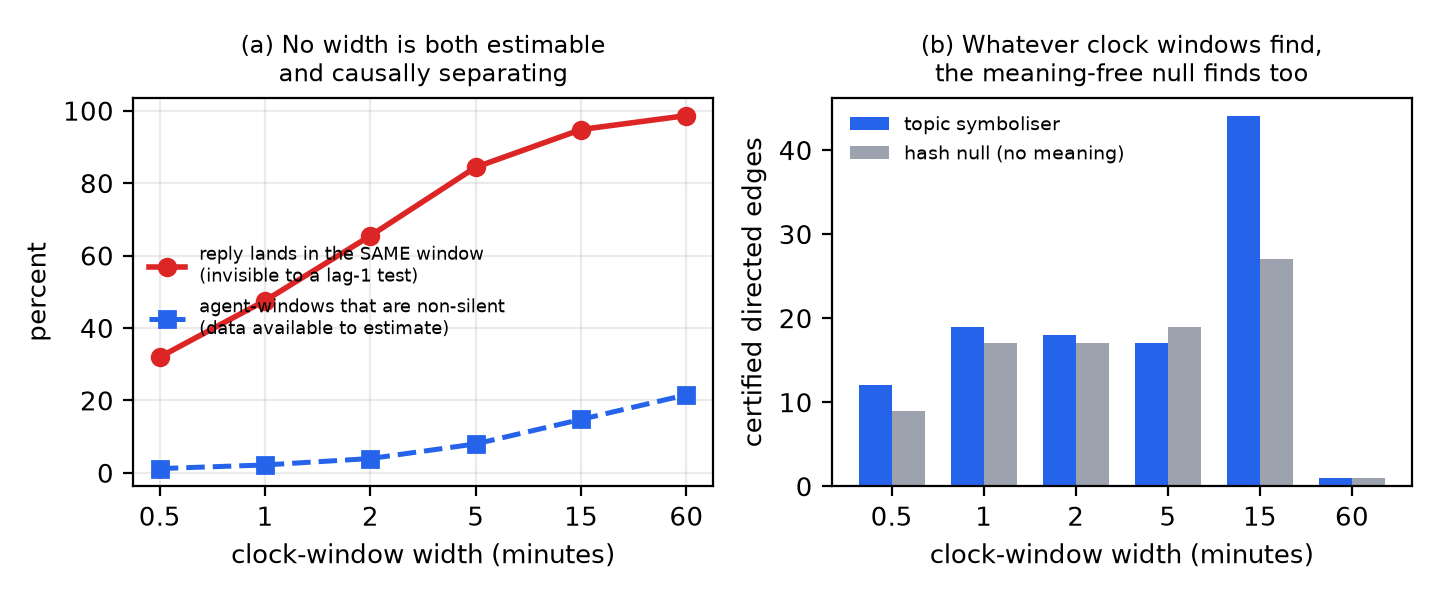
\includegraphics[width=0.92\textwidth]{f1_clock.png}
\caption{Clock-window transfer entropy on the 15 analysed agents of main-village \#general. Left,
the two failure modes as a function of window width. Right, edges certified under the topic
symboliser against the meaning-free hash null.}
\end{figure}

The bind is avoided by ordering messages canonically and letting one message be one tick. Each
agent's series carries its symbol where it spoke and a silent symbol elsewhere, so the lag-1
comparison is between a message and the one immediately before it. The cost is that the measure
captures immediate-predecessor influence only.

\section{The surrogate failure, and two explanations that did not hold}
\label{sec:failure}

An agent is planted into the real stream, drawing its symbols from the channel's marginal and
coupled to nothing at all. It is certified as driving something in 3 of 8 runs when it posts 50
messages, and in 8 of 8 at 100, 263, 600 and 1500 messages, with the mean largest $z$ rising from 5.6
to 12.3, 21.7, 38.3 and 71.7. The error grows with how much the agent speaks, which rules out a
small-sample explanation.

A planted agent could be dismissed as artificial, so the error rate is also measured directly.
Keeping the real speaker sequence and permuting the symbols globally leaves data with no directed
topical influence by construction. The shift surrogate certifies at least one edge in 9 of 10 such
replicates, a family-wise error rate of 0.90 against a nominal 0.05.

\paragraph{What breaks it is the speaker sequence.} Destroying one structure at a time isolates the
cause. Keeping the real speaker order and shuffling only symbols, the shift surrogate fires in 10 of
10 replicates; randomising the speaker order as well drops it to 0 of 10; uniform symbols with the
real order still give 6 of 10. So the driver is the structure of the speaker sequence, not the
symbol distribution and not sparsity. That sequence is far from random in two ways at once: it
repeats a speaker 36\% of the time and returns after one message 38\% of the time, and each agent's
activity is strongly non-stationary, with a median block-share coefficient of variation of 0.79.
Shuffling the order destroys both at once, so this ablation cannot say which of the two mattered.

\subsection{Two explanations I proposed, and the benchmark refuted both}

I initially attributed the failure to mutual exclusivity: only one agent can speak at each tick, so
shifting individual timelines could create overlaps that never occurred in the original
conversation. The benchmark did not support this explanation. A generated channel with exactly one
speaker per tick and steady activity produced an error rate of just 0.025, 95\% Wilson
$[0.011, 0.057]$, far below the 0.90 observed in the real data. Mutual exclusivity alone therefore
cannot explain the failure.

I then suspected turn-taking. In the real channel, speakers repeat 36\% of the time and return after
exactly one message 38\% of the time. However, adding a Markov speaker chain to the generator
produced the opposite result. Turn-taking suppressed the error rather than increasing it. At the
nominal knob values and with no drift the surrogate certified nothing at all across 200 replicates,
while removing turn-taking and introducing drift raised the rate to 0.365. The contribution from
drift was $+0.340$, compared with $-0.025$ for turn-taking. The same inversion appears in the arm
calibrated so that the generated channel reproduces the real channel's measured repeat, return and
block-share statistics rather than merely carrying those numbers as settings: there, turn-taking
alone also certifies nothing, and drift alone gives 0.065.

Neither mechanism, nor their combination in the tested design, reproduced the real-data error rate of
0.90. The largest cell anywhere in the design is 0.365. The real-data ablation removes turn-taking
and non-stationarity together, while the generator separates them. The results point to
non-stationary activity, but the remaining gap means the mechanism behind the full real-data failure
is not yet established.

Every figure above comes from the run at 200 surrogate draws. The first version of this analysis
used 100, which inflates both nulls on the same 2,400 instances: the circular shift fires 53 times
where the 200-draw run does not, against 18 the other way (exact McNemar $p = 3.9 \times 10^{-5}$),
and the permutation surrogate 83 against 20 ($p = 2.7 \times 10^{-10}$). Every qualitative conclusion
in this section is the same at both settings, which is why they are worth stating at all. The
numbers are not, so the draw count belongs in the caption.

\section{The repair, compared}
\label{sec:repair}

Following the local-permutation idea of \citet{runge2018} as adapted by \citet{shorten2021}, each
source keeps its speaking positions and only its symbols are permuted among them. Speaking pattern,
sparsity and turn-taking are preserved exactly, and only the correspondence between symbol and time
is destroyed. On the same destroyed-structure real data the family-wise error rate falls to 0.063
over 300 replicates, 95\% Wilson $[0.041, 0.097]$. The planted uncoupled agent is never certified: 0
of 5 at both 263 and 1500 messages, with mean max $z$ of 2.8 in each case against 22.0 and 68.3
under the shift surrogate.

\begin{figure}[h]
\centering
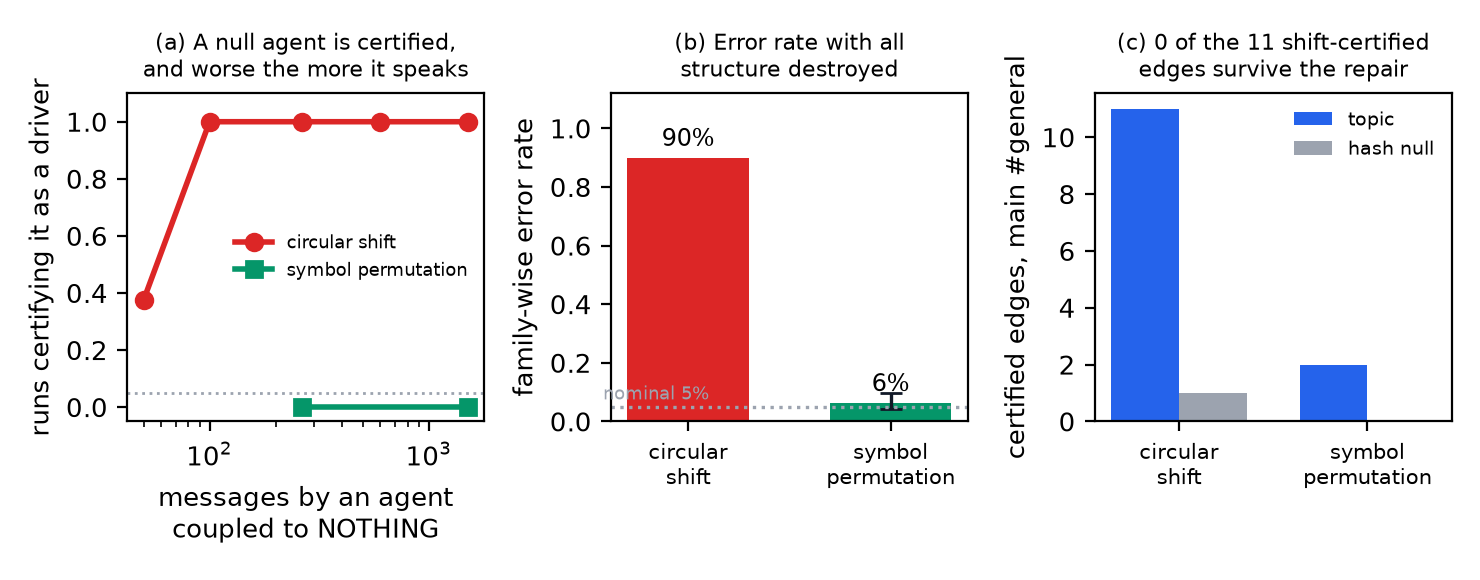
\includegraphics[width=\textwidth]{f2_null.png}
\caption{Left, how often an agent coupled to nothing is certified as a driver, under each surrogate.
Middle, family-wise error rate measured on data with all structure destroyed, with a Wilson
interval; the dotted line is the nominal 0.05. Right, what each surrogate certifies on the real
channel.}
\end{figure}

\subsection{How many surrogate draws are needed}

The number of surrogate draws matters more than I initially appreciated. In a paired comparison of
300 instances, where all four surrogates run on identical symbol grids so the outcomes are paired,
the global permutation surrogate produced a false-positive rate of 0.1167 with 100 draws, falling to
0.0700 with 200 draws, 95\% Wilson $[0.046, 0.105]$. This difference is statistically significant
(exact McNemar $p = 0.0043$). The block-local and Runge local permutations were less sensitive to the
increase: their corresponding rates changed from 0.0900 to 0.0767 and from 0.0967 to 0.0800.

At 200 draws, the global permutation's interval covers the nominal 0.05 and overlaps the real-data
estimate of 0.0633 $[0.0409, 0.0968]$. The real-data result is therefore corroborated rather than
overstated. For practical use, the important point is that reducing the number of surrogate draws
can materially change the result. In particular, the global permutation over-fires at 100 draws by
approximately a factor of two. I would therefore not treat the choice of draw count as a minor
computational detail.

The same correction applies to the benchmark-wide estimate. That figure was 0.0942 at 100 draws.
Repeating all 2,400 instances at 200 draws gives \textbf{0.0679}, 95\% Wilson $[0.0585, 0.0787]$,
and the paired difference is large: 83 instances fire at 100 draws and not at 200, against 20 the
other way, $p = 2.7 \times 10^{-10}$. The conclusion it supports is unchanged, because the interval
still excludes the nominal 0.05. So the permutation repair does carry a residual inflation on clean
generated data, but it is about a third above nominal rather than nearly double.

One limit on this recommendation. I compared 100 draws against 200 and did not test any larger
value, so what the experiment establishes is that 100 is too few, not that 200 is enough. Two
hundred is a lower bound on the draw count rather than a converged setting, and a practitioner whose
conclusions sit near a decision boundary should check their own sensitivity rather than adopt the
number.

\subsection{Choosing a repair, when the error rate cannot choose}

The comparison of the three permutation-based repairs does not produce a clear winner. All four
surrogates were evaluated on identical symbol grids across 300 pure-null replicates, so the
comparison reflects differences between the null models rather than differences between datasets.

\begin{table}[h]
\centering
\begin{tabular}{lrrrl}
\toprule
surrogate & FWER, 100 draws & FWER, 200 draws & 95\% Wilson at 200 & nominal 0.05 \\
\midrule
circular shift                   & 0.0433 & \textbf{0.0333} & $[0.018, 0.060]$ & inside \\
global within-speaker permutation & 0.1167 & \textbf{0.0700} & $[0.046, 0.105]$ & inside \\
block-local permutation          & 0.0900 & \textbf{0.0767} & $[0.052, 0.112]$ & excluded \\
local permutation \citep{runge2018} & 0.0967 & \textbf{0.0800} & $[0.054, 0.116]$ & excluded \\
\bottomrule
\end{tabular}
\caption{Four surrogates on identical symbol grids, 300 pure-null replicates, at both draw counts.}
\end{table}

At 200 draws, paired on the same 300 instances, the circular shift is not significantly different
from the global permutation ($p = 0.0614$), although it differs from block-local permutation
($p = 0.0294$) and from Runge's local permutation ($p = 0.0201$). At 100 draws it differed from all
three, which is the draw-count artifact again. The three repairs remain statistically
indistinguishable from one another, with pairwise $p$-values of 0.85, 0.65 and 1.00. The apparent
differences in their error rates are not sufficient to establish a ranking.

Choosing between them therefore requires more than calibration, and two readings pull against each
other. Runge's local permutation has the strongest methodological justification for preserving the
structure it is intended to preserve, and it follows the approach adapted to event data by
\citet{shorten2021}. Block-local permutation is more heuristic and introduces a free parameter that
has not been tuned. Global permutation is the simplest. On the other hand, the global permutation has
the most favourable interval relative to the nominal rate, and is the only repair that costs nothing
measurable against the shift on clean stationary data, although neither difference is statistically
established. I do not consider the observed error rates sufficient to select one repair over the
others. The choice should be guided by the structure the null is intended to preserve and the
assumptions that can be justified for the data.

\subsection{When to use the repair}

A drift sweep gives the practical reading. Across 150 replicates per cell at 200 surrogate draws,
the circular shift degrades steadily as activity drift increases while the three repairs do not.

\begin{table}[h]
\centering
\begin{tabular}{lrrrr}
\toprule
activity drift & circular shift & global permutation & block-local & local \\
\midrule
0.0 & \textbf{0.013} & 0.093 & 0.080 & 0.093 \\
0.3 & 0.100 & 0.100 & 0.093 & 0.120 \\
0.6 & \textbf{0.193} & 0.053 & 0.047 & 0.067 \\
0.9 & \textbf{0.380} & 0.087 & 0.080 & 0.080 \\
\bottomrule
\end{tabular}
\caption{Family-wise error on pure nulls as activity drift increases, 150 replicates per cell, 200
surrogate draws. Every certified edge is a false positive by construction.}
\end{table}

The pattern is supported by a formal trend test rather than by eye. A Cochran-Armitage test across
the four ordered drift levels gives the circular shift $z = 8.667$, $p < 10^{-15}$, and gives every
repair nothing: $p = 0.51$ for the global permutation, 0.63 for block-local and 0.37 for local. The
same pattern holds at both surrogate draw counts, so it does not depend on that choice.

The repairs are therefore flat under drift rather than calibrated. Only one of the four global
permutation intervals covers the nominal 0.05, and the rest sit nearer 0.09, so what the repair buys
is insensitivity to drift rather than correctness. One asymmetry should be stated rather than
hidden: block-local covers nominal in three of the four cells where the global repair covers one.
The two remain pairwise indistinguishable, so this is not grounds to switch the recommendation, but
it does mean the global repair cannot be described as the best-calibrated under drift.

The results also show why the repair should not be treated as universally preferable. At zero drift
the circular shift has an error rate of 0.013, while the three repairs are all around 0.08 to 0.09.
That advantage is gone by the first drift step: at drift 0.3 the shift reads 0.100 against the global
permutation's 0.100 and block-local's 0.093, so the crossover falls between drift 0.0 and 0.3 rather
than at some higher level. By drift 0.6 the shift is roughly four times the repairs. If a channel has
been checked and found stationary, the circular shift may be sufficient. When activity is
non-stationary the repairs are the more stable choice, and the margin for error on that judgement is
narrow, because the crossover arrives by the first drift level tested.

\section{Continuous time, and what the repair cannot test}

An earlier analysis identified continuous-time estimation as the principled option for event data
but did not evaluate it. Running the continuous-time estimator CoTETE on both channels certifies 0
edges in either case, compared with 2 for main-village and 18 for open-chat under the discrete,
turn-ordered analysis. Its highest $z$-scores are 3.062 and 3.980, below the respective max-T
thresholds of 4.171 and 4.308.

At first these results might appear to contradict the symbol-based analysis. The two estimators
operate on different information, however. CoTETE's public API takes event times with no symbol
channel, while the transfer-entropy analysis here uses topic symbols. To test whether this
difference explains the results, I reduced the data to timing alone, replacing every spoken symbol
with the same code. Under this representation the estimator used here also detects 0 edges in both
channels, matching CoTETE. Using the circular-shift surrogate instead produces 12 and 3 edges. So
neither method detects relationships from event timing alone in these channels, and the edges found
by the symbol-based analysis depend on symbol correspondence, which the continuous-time estimator
cannot access.

Two caveats attach to those $z$-scores, and the second attaches to the larger of them. Point
estimates from this estimator are stochastic to about 17\% across repeated runs, so none of these
values should be read to more than two significant figures. And open-chat's highest $z$, the 3.980,
belongs to the one pair whose surrogate draws mostly failed: it needed 1,936 failed draws to obtain
100 successes, a 4.9\% success rate. Those surrogates are conditioned on being estimable, so that
pair's null is biased in an unknown direction. The conclusion does not rest on it, since that pair
falls below threshold and so does every other pair, but the number should not be quoted as a clean
measurement. The failures themselves were a defect rather than a property of the data: an enlarged
exclusion window can empty the neighbour search on sparse bursty event trains and raise an error
that terminates a whole pair, with no handling at the public entry point. This has been reported
upstream.

There is also a fundamental limitation in applying the recommended permutation surrogate to
timing-only data. When every event carries the same symbol, permuting those symbols changes nothing.
The observed statistic and the surrogate null are identical, making the test exactly degenerate:
standard deviation 0 across all 210 pairs and $p = 1.0$ everywhere. \textbf{The repair has zero power
against timing structure by construction.} The permutation surrogate is appropriate for testing
relationships in the symbol sequence, but it does not answer whether relationships exist in event
timing. These are different questions, and choosing one null means giving up the ability to test the
other with that procedure.

\section{Confounding, and what conditioning removes}

A valid surrogate fixes calibration but not confounding. If every agent tracks a drifting channel
topic, every pair is genuinely dependent through the channel, and pairwise transfer entropy cannot
tell that from direct influence. I therefore also report a \textbf{conditional} estimate, which asks
whether a source's last message adds anything about a target's next one beyond the target's own
history and the channel's recent state. The conditioning variable is the modal symbol of the last
twelve messages, excluding the immediately preceding one so that it does not simply restate the
source.

On a generated benchmark whose decisive instances contain no influence while every agent tracks a
shared drifting topic, so that any certified edge is common cause, pairwise transfer entropy
certifies \textbf{22.3} edges on average and conditioning takes that to \textbf{0.33}, lifting pooled
precision on the four-edge instances from 0.17 to \textbf{0.80} at a recall of 1.0 either way. Across
couplings from 0.05 to 0.8 the conditional test still finds the planted edge in 3 of 3 runs, so the
gain costs no power.

The benchmark flatters the conditional estimator, since its common cause is a shared modal topic and
the conditioning variable is the channel's modal topic. The real channels are harder, and
conditioning there costs degrees of freedom: a 9-symbol alphabet with a 9-valued context gives 6,561
cells against about 7,900 ticks, so that variable is also coarsened to 4 and 2 values.

\begin{table}[h]
\centering
\begin{tabular}{lrrrr}
\toprule
channel & pairwise & conditional, 9 values & 4 values & 2 values \\
\midrule
main \#general      & 2  & \textbf{2, the same two edges} & 2 & 3 \\
open-chat \#general & 18 & \textbf{0} & \textbf{7} & \textbf{13} \\
swarm, room a       & 1  & \textbf{0} & & \\
\bottomrule
\end{tabular}
\caption{Conditioning at three resolutions. Main-village's two edges are robust to that choice;
open-chat's zero is not.}
\end{table}

At the finest resolution the open-chat test is degenerate, its surrogate sitting above the observed
statistic for 65\% of pairs with the largest $z$ in the family only 4.4, so it is failing to reject
rather than finding nothing to reject. Open-chat's structure therefore remains
\textbf{undetermined}: depending on the conditioning resolution, between 0 and 13 of its 18 edges may
survive. That resolution is a free parameter an analyst would set once and never revisit. This is a
property of the channel rather than the estimator: on structure-free real data the conditional test
fires in 2 of 40 replicates, an error rate of 0.05 with a mean $z$ of $-0.001$, so it is nominal
rather than conservative.

\section{The symbolisation floor}
\label{sec:floor}

Everything these methods produce is downstream of turning text into symbols. On the benchmark, where
the underlying topics are known, detection performance drops sharply when agreement between the
symboliser and the ground truth falls below roughly ARI 0.44, and this behaviour appears across the
tested estimators. Importantly, the false-positive rate can look \emph{better} below this point,
because the shared topic structure needed to produce confounded detections is no longer represented
reliably. A pipeline that stops detecting relationships may therefore have lost the signal it needs
rather than become more reliable, and nothing downstream of the symboliser can tell those apart.

\subsection{Detecting the floor without labels}

That degradation can be detected without ground-truth labels. Across the nine-level benchmark sweep,
three statistics separate the below-floor cases with zero errors: seed stability at a threshold of
0.623, agreement with LSA at 0.646, and the Calinski-Harabasz index at 138.9. Seed stability here is
the \textbf{minimum} pairwise agreement across seeds, not the mean; the mean variant makes one error,
at a different threshold of 0.791. Silhouette has the strongest correlation with true ARI, at 0.979,
but is not useful for identifying the boundary because its threshold falls within a gap of just
0.002. A statistic that tracks clustering quality most closely is not necessarily the best one for
making a classification decision.

Error count cannot choose among the three that were perfect, so I tested whether each threshold still
means what it meant when the channel changes for reasons other than topic separability. Applying each
cut unchanged to thirty cells that vary turn-taking, drift, agent count, volume skew, message length
and corpus size, twenty-seven of which hold true ARI at exactly 1.000:

\begin{table}[h]
\centering
\begin{tabular}{lrrrr}
\toprule
diagnostic & cut & errors where fitted & errors, nuisance set & of those at true ARI 1.000 \\
\midrule
seed stability, min across seeds & 0.623 & 0 & 2 & \textbf{0} \\
LSA agreement                    & 0.646 & 0 & 2 & \textbf{0} \\
Calinski-Harabasz                & 138.9 & 0 & 6 & \textbf{3} \\
\bottomrule
\end{tabular}
\caption{Whether a cut fitted on the vocabulary-overlap mechanism survives a change in the channel
that is not a change in topic separability.}
\end{table}

The two bounded statistics err only on the short-message cells, where the symbolisation genuinely has
degraded. Calinski-Harabasz additionally condemns all three cells whose true ARI is exactly 1.000,
for no reason beyond the corpus holding 2,000 messages rather than 8,000, where it reads 76 to 77
against its own cut of 138.9. It is unbounded and grows with sample size, so a published numeric
threshold for it carries no meaning on another corpus. That is why I recommend the two bounded
statistics and not the index that matched them on error count. \textbf{A cut that moves with the
corpus is not a floor cut.}

This is not a weak statistic being discarded on a technicality. Calinski-Harabasz correlates with
true ARI at 0.973, almost as closely as silhouette, and unlike silhouette it classifies the floor
perfectly where it was fitted. It still cannot carry a published threshold. That is the sharper form
of the point above: neither the statistic that tracks quality most closely nor the one that
classifies best on the fitting mechanism is necessarily the one whose cut another researcher can
reuse.

There are important limits to this result. The effective sample size is nine rather than 54, because
the classification label is determined by overlap level. There are no observations between ARI 0.444
and 0.222, so the exact location of the boundary within that interval remains unknown. These
diagnostics classify whether a result is below the tested detection floor; they do not estimate ARI,
and their behaviour is flat between 0.68 and 1.00, and not even monotone there. The benchmark also
uses a single degradation mechanism with a known and correct value of $k$, whereas the true number of
topics in real conversations is unknown. I therefore treat 0.44 as a benchmark-specific, bracketed
result rather than a universal threshold.

\subsection{A contradiction the diagnostic lost}

I initially used these diagnostics to classify one real channel, open-chat, as below the
symbolisation floor. That conclusion did not agree with the channel's measured results: open-chat
certified 18 and 22 edges under the two symbolisers, compared with 2 and 1 for main-village, and its
hash-based null certified zero edges. Rather than treating this disagreement as evidence that the
original measurements were wrong, I revisited the diagnostic itself.

The problem was the choice of $k$. Repeating the comparison with the same channels, loader and window
reproduced the published $k=8$ results to the digit. At $k=4$, however, open-chat reached stability
scores of 0.950 and 0.978, the highest values produced by either channel across the tested settings,
and both exceeded the diagnostic thresholds. The earlier below-floor classification was therefore a
conclusion about one arbitrary choice of $k$, not a reliable statement about the channel. Message
length does not explain the difference either: 27.1\% of main-village messages contain fewer than
five tokens, compared with 2.3\% in open-chat, so the short-message channel is the one the diagnostic
cleared.

This correction changes how the symbolisation results should be read, and it withdrew three claims.

\begin{enumerate}
\item \textbf{The claim that no topic signal remains below the floor is too strong.} The
circular-shift surrogate recovers all four planted edges at every tested overlap level, including
0.95, where ARI is 0.011. The observed collapse is in the permutation null, not necessarily in the
underlying data.
\item \textbf{ARI 0.44 cannot be treated as a universal detection threshold.} When the shared-topic
parameter is 0, detection continues down to ARI 0.296, so the boundary depends on both the
symboliser and the channel.
\item \textbf{Edge counts cannot be used as a measure of symboliser quality.} Even at ARI exactly
1.000, changing the shared-topic parameter alone moves the permutation edge count from 5 to 78.
\end{enumerate}

The diagnostics also do not transfer reliably outside the mechanism on which they were evaluated.
Their balanced accuracy falls from 1.00 to 0.75 and 0.571 under a known mismatch in $k$. All seven
errors made by seed stability are false below-floor classifications, and in every one of those cases
the detector still identifies all planted edges; of the fourteen cells it condemned, eleven had full
conditional recall. The failure direction is the dangerous one: it condemns working symbolisations.

This was an important correction to my own interpretation. I introduced a diagnostic to check whether
the symbolisation was reliable, applied it to the real channels, and found that it contradicted
measurements already in hand. Investigating that contradiction showed the diagnostic was sensitive to
an arbitrary modelling choice. The result is not that the original measurements were wrong, but that
the control was being asked to support a broader conclusion than the evidence allowed. These
diagnostics remain useful within their tested setting, and \textbf{no channel-level floor verdict
should be issued from a single $k$}.

\section{The benchmark}

Real logs have no ground truth, so the common-cause question could not be settled on them. The
generator used here makes the influence graph known by construction: it decides, in code, who speaks
at which tick, on which topic, and who reacts to whom. Surface text is a separate, replaceable layer
drawn from disjoint per-topic vocabularies, so the whole thing runs offline and a detector still has
to symbolise raw text rather than read the labels. Turn-taking and activity drift are independent
knobs, so the two can be varied one at a time, and the generator reproduces its earlier behaviour
bit for bit when both are zero.

\benchname{} is released with 150 tests covering the generator, the detector harness, the text layer,
the floor analysis and the turn-taking factorial.
\ifdeanon{Code and benchmark:
\url{https://github.com/manunicholasjacob/swarm-influence-bench} and
\url{https://github.com/manunicholasjacob/swarm-influence-audit}.}{Code and benchmark are publicly
released; the links are withheld here for anonymity and will be given in the camera-ready version.}

One property of the benchmark must be stated when its numbers are quoted. Planting an edge displaces
other agents' speaking turns, so the generated instances contain real lag-1 dependencies that the
label set does not list. Precision measured against those labels is therefore a \textbf{lower bound}
for any detector, and what the benchmark supports is the comparison between two estimators rather
than the absolute value of either.

\section{What an overseer should do}

Six inexpensive controls should be included whenever an influence graph over an agent channel is
published.

\begin{enumerate}
\item \textbf{Plant an agent coupled to nothing, at your channel's volumes, and check it is not
certified.} This one test would have caught the failure reported here, at one run per volume.
\item \textbf{Measure the error rate directly}, by destroying the structure your method claims to
find and checking the family-wise rate is near nominal. If it is not, your surrogate does not match
your data.
\item \textbf{Preserve the speaker sequence in your surrogate.} Any surrogate that moves an agent's
messages in time will disturb it, and \citet{shorten2021} is the principled route. Use at least 200
surrogate draws, because at 100 the global within-speaker permutation over-fires by roughly a factor
of two.
\item \textbf{Establish the detection floor before interpreting an absence.} ``No edges'' and ``no
influence'' are different claims.
\item \textbf{Condition on the channel, report both numbers, and sweep the resolution.} Pairwise and
conditional bound the answer, and the gap between them is the result. Conditioning costs cells, so
check whether your answer is an artifact of how finely you conditioned. On one channel here it was.
\item \textbf{Report how well your symboliser agrees with the truth, on data where you know it.}
Everything is downstream of turning text into symbols, and below roughly ARI 0.44 detection
collapses whatever the estimator. I have found this control in no influence-detection paper, and it
is also the one that cannot be run on real logs, which is why the floor remains the largest
unquantified threat here.
\end{enumerate}

Two habits follow: publish a meaning-free null's count beside the real one, and require held-out
replication before calling a graph a structure.

\section{The real channels, and what survives}

Re-running every channel under the repaired surrogate changes the answers, and not in one direction.

\begin{table}[h]
\centering
\begin{tabular}{lrrr}
\toprule
channel & window messages & shift: topic / hash & permutation: topic / hash \\
\midrule
main \#general      & 8,800 & 11 / 1 & 2 / 0 \\
open-chat \#general & 8,226 & 3 / 0  & 18 / 0 \\
swarm, room a       & 3,846 & 2 / 1  & 1 / 0 \\
\bottomrule
\end{tabular}
\caption{The same channels under both surrogates, with the meaning-free hash null beside each.}
\end{table}

In main-village, \textbf{none} of the 11 edges the standard recipe certifies survives the repair, and
the two the valid surrogate certifies were not among them. In open-chat the correction runs the other
way, 3 edges becoming 18, because pathological pairs inflate the max-T threshold and raise the bar
for everything else. An invalid surrogate does not simply add false positives; it scrambles the
result.

Main-village's two edges are the strongest thing here and they are still not a finding, because they
do not replicate: the adjacent fourteen-day window certifies nothing at all under either estimator.
Given the detection floor, that silence is as consistent with the test sitting near its limit as with
the edges being absent, and the two cannot be separated. Power is governed by how much an agent says
as much as by how strongly it copies, and it is channel-specific: in main-village a planted follower
copying on 80\% of its messages is caught only 1 time in 4, while in open-chat one copying 10\% of
the time is caught 3 times in 4. Replication is weak everywhere: under the standard recipe the
adjacent window shares 1 edge out of 8 and 4, and that edge is also the only one the hash null
certifies. No certified edge in this work replicates out of sample.

\begin{figure}[h]
\centering
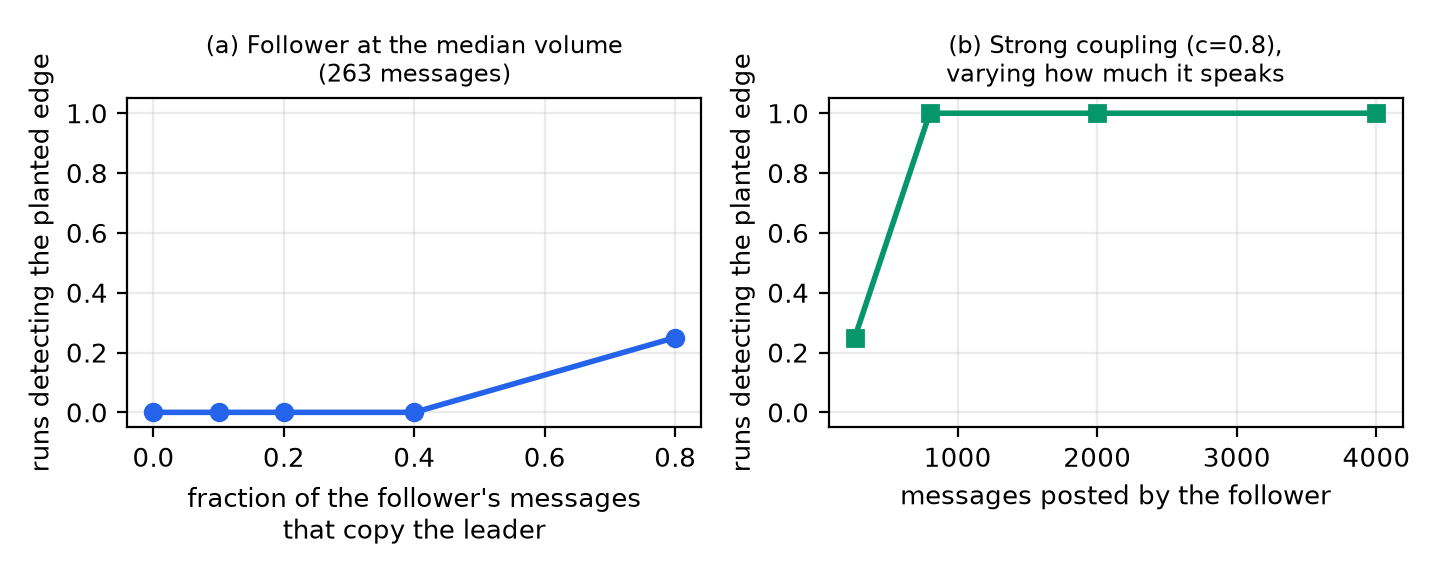
\includegraphics[width=0.92\textwidth]{f4_power.png}
\caption{Detection of a planted follower under the repaired surrogate. Left, varying the fraction of
its messages that copy the leader, at the median agent's volume. Right, varying how much it speaks,
at strong coupling.}
\end{figure}

\paragraph{Humans in the channel.} Main-village \#general is now effectively human-free, with 3 human
messages in the window, so the question has to be asked in open-chat, where 32\% of messages come
from 124 human visitors. Pairwise, with humans collapsed into one node, 19 edges are certified.
Conditioning removes almost all the agent-to-agent structure and little of the rest: \textbf{four
edges survive, of which three run from humans to agents, one is agent to agent, and none run from an
agent to a human.} The asymmetry is not an artifact of the confound. It should be read carefully all
the same: topical dependence from a person to an agent is also what ordinary responsiveness looks
like, so the measurement supports only that the dependence is dyad-specific and directional, not
that anyone is steering a swarm.

\section{Reproducibility, and one limitation of it}

Every number in this paper is recomputed from committed analysis output by a verifier that fails on a
mismatch, and that verifier covers the prose of this paper as well as the figures.

One limitation should be stated plainly. Re-running the counts in the earlier stationarity sweep with
the same seeds and configuration, only one of the eight cells reproduced exactly; the remaining
differences were one or two replicates per cell. Seven of the eight published rates still fell within
the recomputed Wilson intervals, and no conclusion changed. The exception is the zero-drift cell under
the permutation null, where the published 1 of 30 falls just below the recomputed interval of
$[0.035, 0.256]$ for 3 of 30, and no result here depends on that cell.

The generator, estimator and BLAS configuration were investigated and ruled out as the source. The
most likely explanation is a library-level difference, particularly in scikit-learn's $k$-means
implementation within the symboliser, whose output can vary between versions. Every sweep now records
the environment it ran under: Python 3.14.6, numpy 2.5.1, scipy 1.18.0 and scikit-learn 1.9.0,
including the BLAS build and the number of BLAS threads each worker used.

This does not make the previously published counts exactly reproducible. It provides a more clearly
specified environment in which subsequent results can be checked. For that reason I report rates
alongside their confidence intervals rather than exact replicate counts. The distinction between
reproducing a result within its uncertainty and reproducing every individual count matters, and only
the first is claimed.

\section{Conclusion}

Applied to real agent chat, the standard recipe for ``who drives whom'' needs repair before it says
anything. Clock windows cannot separate a message from its answer at the speed agents reply, and what
they certify is matched by a null with no access to meaning. The turn-ordered grid that fixes this
breaks the circular-shift surrogate: family-wise error 0.90 against a nominal 0.05, caused by the
speaker sequence itself. Restricted permutation surrogates repair most of that, but they are flat
under drift rather than calibrated, they are mutually indistinguishable at this precision, and one of
them needs twice the surrogate draws anyone would think to use. A valid surrogate fixes calibration
but not confounding. What survives is small: two dyad-specific edges that do not replicate, an
undetermined answer set by conditioning resolution, and influence running from people into agents and
never back. \textbf{An influence graph should not guide decisions until its error rate, its confound,
its detection floor and its symboliser's fidelity are reported.}

\section*{Limitations}

\begin{itemize}
\item \textbf{Immediate-predecessor only.} The turn-ordered lag-1 measure sees influence from the
message directly before a reply. Influence acting over several turns, or through a room's accumulated
context, is out of scope.
\item \textbf{Discrete approximation to an event process.} Agent chat is event-based in continuous
time. The turn-ordered discretisation with a permutation surrogate is a practical fix, and the
continuous-time comparison above shows what that choice gives up.
\item \textbf{The mechanism behind the real 0.90 is not established.} The generator separates
turn-taking from drift and points at drift, but the largest cell anywhere in the design is 0.365.
\item \textbf{Symbolisation quality cannot be measured on the real logs.} The central result survives
an independent symboliser, but the edge count does not: it moves with alphabet size and with which
messages the topic model is fit on. The floor remains the largest unquantified threat.
\item \textbf{No ground truth in the real logs.} The validity argument rests on planted controls and
on the meaning-free null, not on recovering a known answer.
\item \textbf{Conditioning removes real influence too.} The conditional estimate discards influence
that works by shifting what the channel is talking about, which in a group chat may be a large part
of genuine influence. It is a lower bound on dyadic influence.
\item \textbf{The human result is exploratory.} It rests on one village and one window and should be
read as a lead.
\end{itemize}

\section*{Broader impact and ethics}

This work audits influence detection on a population of AI agents, which is dual-use. Used
defensively it helps an overseer decide what an influence graph is worth, and the main result is
deflationary: it tells practitioners to trust these outputs less, which reduces rather than increases
the chance of acting on a bad attribution. The same tooling could be used to identify the most
influential agent in a swarm in order to target it, or to surveil participants in a channel. Three
properties limit the misuse. The subjects are AI models; the dataset is already public under research
terms and no re-identification is added; and the measure is weak and local, recovering
immediate-predecessor topical dependence rather than any model of how to steer an agent.

The dataset's research terms were followed: research use only, no training on the data, no
re-identification, citation of the source, and notification of the authors of resulting publications.
Human participants appear only as an aggregate node or as anonymised visitor labels, never by name or
handle, and no content attributable to an individual person is reported. Message text and metadata
were read, never model weights or private user data.

The use of a large language model in this work is disclosed in the first-page footnote, as TMLR
requires.

\bibliographystyle{tmlr}
\bibliography{refs}

\end{document}
"               de-anonymised arXiv preprint
%   pdflatex "\def\TMLRMODE{accepted}% TMLR submission. Built 10 November 2026 from:
%   paper/00_PROSE_v1.md   the author's written sections, 78 figures auto-verified
%   report/REPORT_V2.md    the sprint report, every number recomputed by report/verify_v2.py
%
% ANONYMITY. \usepackage{tmlr} with no option is the anonymous submission mode: the tmlr
% package hides the author block itself. Switching to [preprint] de-anonymises for arXiv AND
% turns on the \ifpreprint branches below, which are the only places a name, a repository URL
% or the benchmark's distinctive name appears. So one source produces both documents and the
% anonymous build cannot leak an identifier that the preprint build adds.
%
% Build:  latexmk -pdf main.tex
\documentclass[10pt]{article}

% The mode is chosen at build time so that one source produces every variant and they cannot
% drift apart:
%   latexmk -pdf main.tex                                        anonymous TMLR submission
%   pdflatex "\def\TMLRMODE{preprint}% TMLR submission. Built 10 November 2026 from:
%   paper/00_PROSE_v1.md   the author's written sections, 78 figures auto-verified
%   report/REPORT_V2.md    the sprint report, every number recomputed by report/verify_v2.py
%
% ANONYMITY. \usepackage{tmlr} with no option is the anonymous submission mode: the tmlr
% package hides the author block itself. Switching to [preprint] de-anonymises for arXiv AND
% turns on the \ifpreprint branches below, which are the only places a name, a repository URL
% or the benchmark's distinctive name appears. So one source produces both documents and the
% anonymous build cannot leak an identifier that the preprint build adds.
%
% Build:  latexmk -pdf main.tex
\documentclass[10pt]{article}

% The mode is chosen at build time so that one source produces every variant and they cannot
% drift apart:
%   latexmk -pdf main.tex                                        anonymous TMLR submission
%   pdflatex "\def\TMLRMODE{preprint}% TMLR submission. Built 10 November 2026 from:
%   paper/00_PROSE_v1.md   the author's written sections, 78 figures auto-verified
%   report/REPORT_V2.md    the sprint report, every number recomputed by report/verify_v2.py
%
% ANONYMITY. \usepackage{tmlr} with no option is the anonymous submission mode: the tmlr
% package hides the author block itself. Switching to [preprint] de-anonymises for arXiv AND
% turns on the \ifpreprint branches below, which are the only places a name, a repository URL
% or the benchmark's distinctive name appears. So one source produces both documents and the
% anonymous build cannot leak an identifier that the preprint build adds.
%
% Build:  latexmk -pdf main.tex
\documentclass[10pt]{article}

% The mode is chosen at build time so that one source produces every variant and they cannot
% drift apart:
%   latexmk -pdf main.tex                                        anonymous TMLR submission
%   pdflatex "\def\TMLRMODE{preprint}\input{main}"               de-anonymised arXiv preprint
%   pdflatex "\def\TMLRMODE{accepted}\input{main}"               camera-ready
% Use build.py, which runs all of them and checks the anonymous output for leaks.
\providecommand{\TMLRMODE}{submission}
\makeatletter
\def\@tmlrpreprint{preprint}
\def\@tmlraccepted{accepted}
\ifx\TMLRMODE\@tmlrpreprint
  \usepackage[preprint]{tmlr}
\else
  \ifx\TMLRMODE\@tmlraccepted
    \usepackage[accepted]{tmlr}
  \else
    \usepackage{tmlr}
  \fi
\fi
\makeatother

\usepackage{hyperref}
\usepackage{url}
\usepackage{booktabs}
\usepackage{graphicx}
\usepackage{amsmath}

% Gate every identifying string on whether identity may be revealed at all. The flag to test is
% \if@accepted, NOT \if@preprint: tmlr.sty's [preprint] option sets BOTH, so \if@accepted is true
% for the preprint and the camera-ready and false only for the anonymous submission, which is
% exactly the condition wanted. Gating on \if@preprint alone also hid the repository URLs from the
% camera-ready, which is where this paper promises to give them. \if@accepted is internal to
% tmlr.sty, hence the \makeatletter. The anonymous build takes the second argument.
\makeatletter
\newcommand{\ifdeanon}[2]{\if@accepted#1\else#2\fi}
\makeatother
\newcommand{\benchname}{\ifdeanon{SwarmInfluence-Bench}{the benchmark}}

% An unmarked footnote, for the LLM-use disclosure. TMLR's FAQ requires the disclosure and names
% the location: authors must "mention explicitly in their submission that they have used this
% tool", "as a footnote on the first page". Verified against jmlr.org/tmlr/faq.html on 10 Nov 2026.
% It is therefore not optional, and it does not belong in Broader Impact, where it sat until now.
% Nothing in the policy asks for the vendor's name, so none is given.
\newcommand{\disclosurefootnote}[1]{%
  \begingroup\renewcommand\thefootnote{}\footnote{#1}\addtocounter{footnote}{-1}\endgroup}

\title{An Influence Graph Over AI Agents Certifies an Agent That Copies Nobody}

% Hidden by the tmlr package unless [accepted] or [preprint] is given.
\author{\name Manu Nicholas Jacob \email manunicholasjacob@gmail.com \\
        \addr Independent Researcher}

\def\month{11}
\def\year{2026}
\def\openreview{\url{https://openreview.net/forum?id=XXXXXXXXXX}}

\begin{document}
\maketitle

\begin{abstract}
Circular-shift surrogates can produce severely inflated false-positive rates when applied to
turn-ordered multi-agent conversations, reaching a family-wise error rate of 0.90 against a nominal
0.05. A generated benchmark separates two candidate mechanisms and points at non-stationary speaker
activity rather than turn-taking, which suppresses the failure rather than causing it. No setting of
either knob reproduces the observed 0.90, however, so what drives the full real-data failure remains
open. Restricted permutation surrogates substantially reduce the problem. Their error rate is flat
with respect to drift rather than at the nominal level, and for the global within-speaker variant it
depends on how many surrogate draws the null is built from. Calibration alone does not address
confounding, which motivates a conditional estimator validated against a benchmark with planted
ground truth. I also identify a symbolisation-dependent detection limit and develop label-free
diagnostics for it, and show that their calibration does not transport across degradation
mechanisms. The benchmark is released.
\end{abstract}

\disclosurefootnote{\textbf{Use of a large language model.} A large language model was used as an
assistive tool: to help write and run the analysis code, and to help draft this paper. The author is
responsible for every claim, number and figure. All results come from the released code run on the
public dataset, no result or reference is fabricated, and every number in this paper is recomputed
from committed analysis output by a verifier that fails the build on a mismatch.}

\section{Introduction}

When AI agents interact in a shared channel, it is useful to understand how they influence one
another. Information-theoretic methods offer a way to measure this through lagged transfer entropy,
surrogate testing, and per-agent influence scores. They are attractive because they require no
labels and no access to model internals, only a record of who said what and when. The reliability of
those measurements is what this paper examines.

Almost every demonstration of these detectors runs on synthetic traces with a planted leader, where
the analyst controls timing and vocabulary. Real agent chat is asynchronous, bursty, and written in
open language. The narrower question here is whether the standard recipe, applied to real agent
logs, returns anything an overseer should act on.

The audit runs on the AI Village corpus \citep{aidigest2026}, in which frontier models share chat
channels over eighteen months across four villages differing in size, lifetime and tempo, applying
the checks a reader should demand: planted controls, a meaning-free symboliser, replication in a
held-out window, and sensitivity to every parameter that had to be chosen.

\begin{enumerate}
\item The conventional circular-shift surrogate is \textbf{invalid} on turn-ordered agent chat: a
family-wise error rate of 0.90 against a nominal 0.05, caused by the structure of the speaker
sequence itself.
\item Restricted permutation surrogates restore most of the calibration, and re-certifying under one
\textbf{scrambles rather than shrinks} the answer: one channel loses all 11 of its edges, another
gains 15.
\item The three restricted variants are \textbf{mutually indistinguishable} at the precision reached
here, so the choice between them cannot be justified on error rate. The global within-speaker
variant additionally needs on the order of 200 surrogate draws, and over-fires by roughly a factor
of two at 100.
\item Calibration is not confounding, so a conditional estimate is added and validated on a released
benchmark with a known influence graph: common-cause false edges fall from 22.3 to 0.33, and on the
planted-edge instances precision rises from 0.17 to 0.80 with no loss of recall or power.
\item The same benchmark exposes a \textbf{symbolisation floor}. Below roughly 0.44 adjusted Rand
index between symboliser and truth, detection collapses whatever the estimator. Label-free
diagnostics detect that floor, but their calibration does not transport across degradation
mechanisms, and I report where it fails.
\item On the real channels two edges stand at every conditioning resolution, 18 are
\textbf{undetermined} between 0 and 13, none replicates out of sample, and what survives alongside
humans runs from people to agents.
\end{enumerate}

\section{Related work}

\paragraph{Transfer entropy and surrogates.} Transfer entropy \citep{schreiber2000} measures how much
a source's past reduces uncertainty about a target's next symbol beyond the target's own past.
Plug-in estimators are biased upward on short series, so significance rests on surrogate data, with
family-wise error controlled by a max-T test \citep{westfall1993}. The usual surrogate is a circular
time shift of the source.

\paragraph{Event-based data breaks the shift surrogate.} \citet{shorten2021}, on neural spike trains,
show that the conventional source-time-shift surrogate fails to represent the null hypothesis of
conditional independence for event-based processes, and adapt to that setting the nearest-neighbour
local permutation scheme of \citet{runge2018}. Agent chat is event-based in that sense: messages are
events in continuous time, not samples of a clocked signal. The correction is not a contribution of
this paper. The contribution is showing that the same failure carries over to multi-agent safety
monitoring, and that it can be severe enough to create apparent leaders where none exist.

\paragraph{The same failure, concurrently, in multi-agent reinforcement learning.}
\citet{papadopoulos2026} report a closely related surrogate failure in multi-agent
reinforcement-learning action series. Their agent pairs have zero influence by construction, yet
circular time shifts produce false-positive rates of 100\% and 98.2\% against a nominal 0.05. A
plain permutation surrogate fares no better in their setting, at 100.00\% and 99.95\%. Their
proposed correction restricts permutations to blocks of training time, which returns the rates to
5.25\% and 5.50\%.

There are important differences between their setting and this one. Their data consist of binary
actions recorded over twelve thousand training rounds, whereas these data are symbolised
natural-language messages arranged on a turn-ordered conversational grid. Their non-stationarity
comes from monotone drift associated with annealing exploration; here the relevant non-stationarity
appears in the speaker sequence. Neither result should be taken as a direct extension of the other.

Nevertheless, the fact that both approaches rely on restricted permutations is worth noting. Their
permutation blocks are defined by training time, while mine are defined by an agent's own speaking
positions. This provides convergent evidence that unrestricted temporal rearrangement can be
problematic in non-stationary multi-agent data. Their findings also serve as a useful warning for
the approach taken here, and the warning has a measured form rather than a rhetorical one: in their
data the unrestricted permutation failed as completely as the time shift, at 100.00\% against a
nominal 0.05. Permutation-based surrogates are not automatically protected against
non-stationarity, and what protects the one used here is the restriction, not the permutation. I
claim no priority over their result and view the two studies as complementary, addressing different
forms of structured multi-agent data.

\paragraph{Oversight under a budget.} AI-control research frames monitoring as resource constrained,
with a cost for false positives \citep{greenblatt2024}. An influence graph is one such measurement,
and its error rate is the concern here.

\paragraph{Clustering stability.} The idea of using clustering stability as a label-free quality
indicator is not new. It has a substantial history, including \citet{benhur2002},
\citet{lange2004}, von Luxburg's review of clustering stability \citep{vonluxburg2010}, and
\citet{tibshirani2005} on prediction strength. What is different in Section~\ref{sec:floor} is the
calibration of these diagnostics against a detection-performance floor rather than against cluster
recovery alone.

\section{Data and representation}

The AI Village dataset ships one gzipped-JSONL table per village. Four villages are used, differing
enough to test whether any finding is a property of one channel.

\begin{table}[h]
\centering
\begin{tabular}{lrrrrl}
\toprule
village & agent messages & agents & lifetime & human messages & busiest room \\
\midrule
main      & 205,726 & 58  & 576 days & 10,029 & \#general (166,715, 81\%) \\
open-chat &  35,483 & 23  &  66 days & 12,264 & \#general (all) \\
swarm     &   3,848 & 133 &   1 day  &      5 & room a (3,846) \\
game-jam  &     838 & 6   &   3 days &     36 & per-team rooms \\
\bottomrule
\end{tabular}
\caption{The four villages. A 2026 scaffolding change scopes each agent to its current room's
context, so the busiest room of each village is a self-contained influence substrate and is analysed
alone.}
\end{table}

The primary window is the final fourteen days of main-village \#general, 17 to 31 October 2026,
holding 8,800 agent messages. Twenty-two models posted at least 50 messages each and the directed
test uses the 15 busiest, giving 7,958 message events. Two scaffolding facts are disclosed rather
than corrected: the automated nudger was off throughout, and the unused \#best and \#rest rooms were
soft-deleted mid-window, which does not touch \#general.

\subsection{From open language to symbols}

Transfer entropy needs discrete symbols, so each message is mapped to a small alphabet before
influence is estimated, and that mapping is kept separate from the estimator. A topic symboliser
(TF-IDF then $k$-means, $k=8$) gives a message its topic cluster id, so paraphrases of one idea share
a symbol. A hash symboliser, a stable hash of the normalised text into $k=8$ buckets, has no notion
of meaning and serves as a null: an edge appearing under both lives in timing alone.

\subsection{The lag problem, and why clock windows cannot solve it}

A lag-1 transfer entropy compares window $t-1$ with window $t$, so influence landing inside one
window is invisible to it. Agent chat makes this binding. Among the fifteen analysed agents the gap
between consecutive messages by different speakers has a median of 28.1 seconds (25th percentile
9.2, 75th 66.2, 95th 159.3), so turn-taking is a seconds-scale process while any clock window wide
enough to hold two speakers is minutes wide and swallows both a message and its answer.

Both horns are measurable. At 30 seconds only 1.2\% of agent-windows hold a message, while 32.0\% of
replies already land in the same window as what they answer, rising to 84.4\% at five minutes. At
every width tried, the meaning-free hash null certifies comparably many edges, and more at five
minutes: 9 against 12 at thirty seconds, 17 against 19 at one minute, 27 against 44 at fifteen, and
19 against 17 at five. Whatever clock-window transfer entropy was detecting there, it was not shared
meaning.

\begin{figure}[h]
\centering
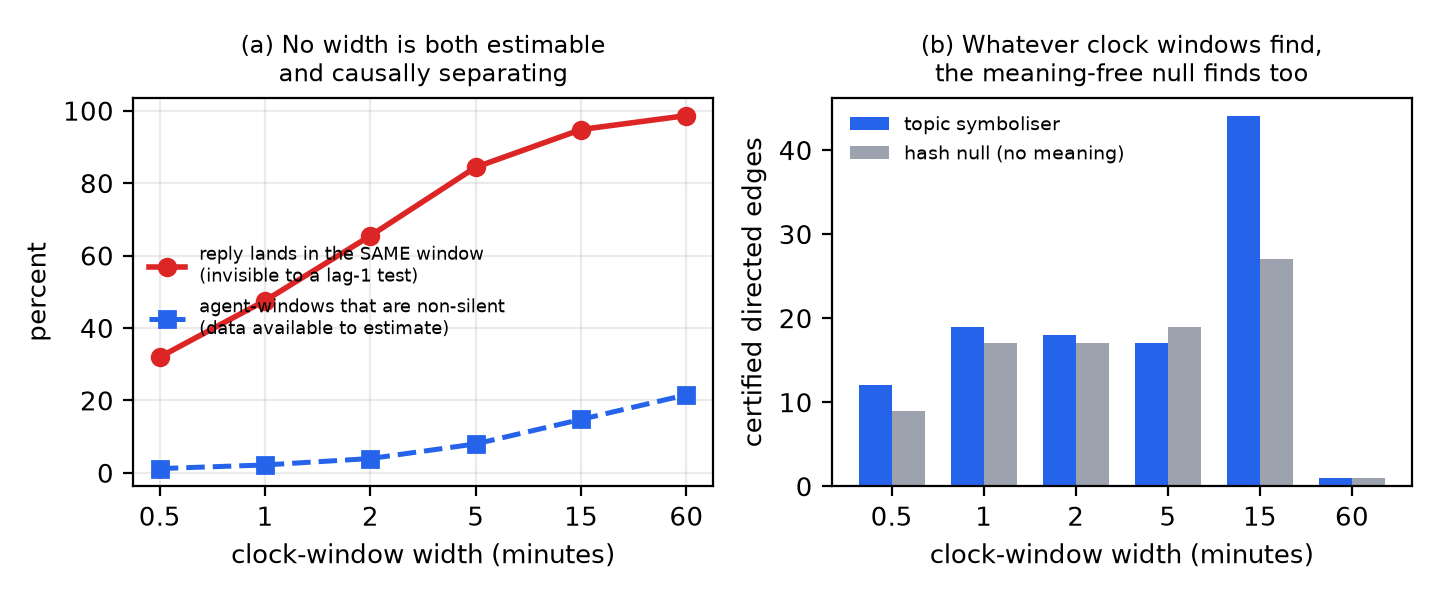
\includegraphics[width=0.92\textwidth]{f1_clock.png}
\caption{Clock-window transfer entropy on the 15 analysed agents of main-village \#general. Left,
the two failure modes as a function of window width. Right, edges certified under the topic
symboliser against the meaning-free hash null.}
\end{figure}

The bind is avoided by ordering messages canonically and letting one message be one tick. Each
agent's series carries its symbol where it spoke and a silent symbol elsewhere, so the lag-1
comparison is between a message and the one immediately before it. The cost is that the measure
captures immediate-predecessor influence only.

\section{The surrogate failure, and two explanations that did not hold}
\label{sec:failure}

An agent is planted into the real stream, drawing its symbols from the channel's marginal and
coupled to nothing at all. It is certified as driving something in 3 of 8 runs when it posts 50
messages, and in 8 of 8 at 100, 263, 600 and 1500 messages, with the mean largest $z$ rising from 5.6
to 12.3, 21.7, 38.3 and 71.7. The error grows with how much the agent speaks, which rules out a
small-sample explanation.

A planted agent could be dismissed as artificial, so the error rate is also measured directly.
Keeping the real speaker sequence and permuting the symbols globally leaves data with no directed
topical influence by construction. The shift surrogate certifies at least one edge in 9 of 10 such
replicates, a family-wise error rate of 0.90 against a nominal 0.05.

\paragraph{What breaks it is the speaker sequence.} Destroying one structure at a time isolates the
cause. Keeping the real speaker order and shuffling only symbols, the shift surrogate fires in 10 of
10 replicates; randomising the speaker order as well drops it to 0 of 10; uniform symbols with the
real order still give 6 of 10. So the driver is the structure of the speaker sequence, not the
symbol distribution and not sparsity. That sequence is far from random in two ways at once: it
repeats a speaker 36\% of the time and returns after one message 38\% of the time, and each agent's
activity is strongly non-stationary, with a median block-share coefficient of variation of 0.79.
Shuffling the order destroys both at once, so this ablation cannot say which of the two mattered.

\subsection{Two explanations I proposed, and the benchmark refuted both}

I initially attributed the failure to mutual exclusivity: only one agent can speak at each tick, so
shifting individual timelines could create overlaps that never occurred in the original
conversation. The benchmark did not support this explanation. A generated channel with exactly one
speaker per tick and steady activity produced an error rate of just 0.025, 95\% Wilson
$[0.011, 0.057]$, far below the 0.90 observed in the real data. Mutual exclusivity alone therefore
cannot explain the failure.

I then suspected turn-taking. In the real channel, speakers repeat 36\% of the time and return after
exactly one message 38\% of the time. However, adding a Markov speaker chain to the generator
produced the opposite result. Turn-taking suppressed the error rather than increasing it. At the
nominal knob values and with no drift the surrogate certified nothing at all across 200 replicates,
while removing turn-taking and introducing drift raised the rate to 0.365. The contribution from
drift was $+0.340$, compared with $-0.025$ for turn-taking. The same inversion appears in the arm
calibrated so that the generated channel reproduces the real channel's measured repeat, return and
block-share statistics rather than merely carrying those numbers as settings: there, turn-taking
alone also certifies nothing, and drift alone gives 0.065.

Neither mechanism, nor their combination in the tested design, reproduced the real-data error rate of
0.90. The largest cell anywhere in the design is 0.365. The real-data ablation removes turn-taking
and non-stationarity together, while the generator separates them. The results point to
non-stationary activity, but the remaining gap means the mechanism behind the full real-data failure
is not yet established.

Every figure above comes from the run at 200 surrogate draws. The first version of this analysis
used 100, which inflates both nulls on the same 2,400 instances: the circular shift fires 53 times
where the 200-draw run does not, against 18 the other way (exact McNemar $p = 3.9 \times 10^{-5}$),
and the permutation surrogate 83 against 20 ($p = 2.7 \times 10^{-10}$). Every qualitative conclusion
in this section is the same at both settings, which is why they are worth stating at all. The
numbers are not, so the draw count belongs in the caption.

\section{The repair, compared}
\label{sec:repair}

Following the local-permutation idea of \citet{runge2018} as adapted by \citet{shorten2021}, each
source keeps its speaking positions and only its symbols are permuted among them. Speaking pattern,
sparsity and turn-taking are preserved exactly, and only the correspondence between symbol and time
is destroyed. On the same destroyed-structure real data the family-wise error rate falls to 0.063
over 300 replicates, 95\% Wilson $[0.041, 0.097]$. The planted uncoupled agent is never certified: 0
of 5 at both 263 and 1500 messages, with mean max $z$ of 2.8 in each case against 22.0 and 68.3
under the shift surrogate.

\begin{figure}[h]
\centering
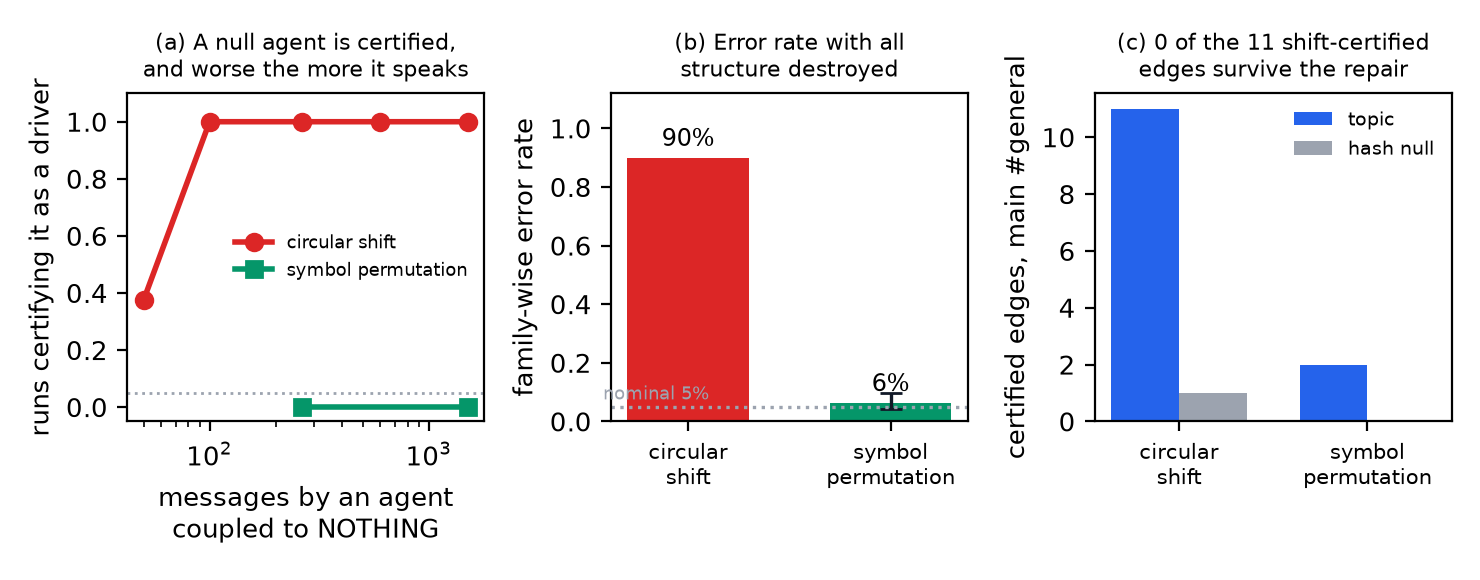
\includegraphics[width=\textwidth]{f2_null.png}
\caption{Left, how often an agent coupled to nothing is certified as a driver, under each surrogate.
Middle, family-wise error rate measured on data with all structure destroyed, with a Wilson
interval; the dotted line is the nominal 0.05. Right, what each surrogate certifies on the real
channel.}
\end{figure}

\subsection{How many surrogate draws are needed}

The number of surrogate draws matters more than I initially appreciated. In a paired comparison of
300 instances, where all four surrogates run on identical symbol grids so the outcomes are paired,
the global permutation surrogate produced a false-positive rate of 0.1167 with 100 draws, falling to
0.0700 with 200 draws, 95\% Wilson $[0.046, 0.105]$. This difference is statistically significant
(exact McNemar $p = 0.0043$). The block-local and Runge local permutations were less sensitive to the
increase: their corresponding rates changed from 0.0900 to 0.0767 and from 0.0967 to 0.0800.

At 200 draws, the global permutation's interval covers the nominal 0.05 and overlaps the real-data
estimate of 0.0633 $[0.0409, 0.0968]$. The real-data result is therefore corroborated rather than
overstated. For practical use, the important point is that reducing the number of surrogate draws
can materially change the result. In particular, the global permutation over-fires at 100 draws by
approximately a factor of two. I would therefore not treat the choice of draw count as a minor
computational detail.

The same correction applies to the benchmark-wide estimate. That figure was 0.0942 at 100 draws.
Repeating all 2,400 instances at 200 draws gives \textbf{0.0679}, 95\% Wilson $[0.0585, 0.0787]$,
and the paired difference is large: 83 instances fire at 100 draws and not at 200, against 20 the
other way, $p = 2.7 \times 10^{-10}$. The conclusion it supports is unchanged, because the interval
still excludes the nominal 0.05. So the permutation repair does carry a residual inflation on clean
generated data, but it is about a third above nominal rather than nearly double.

One limit on this recommendation. I compared 100 draws against 200 and did not test any larger
value, so what the experiment establishes is that 100 is too few, not that 200 is enough. Two
hundred is a lower bound on the draw count rather than a converged setting, and a practitioner whose
conclusions sit near a decision boundary should check their own sensitivity rather than adopt the
number.

\subsection{Choosing a repair, when the error rate cannot choose}

The comparison of the three permutation-based repairs does not produce a clear winner. All four
surrogates were evaluated on identical symbol grids across 300 pure-null replicates, so the
comparison reflects differences between the null models rather than differences between datasets.

\begin{table}[h]
\centering
\begin{tabular}{lrrrl}
\toprule
surrogate & FWER, 100 draws & FWER, 200 draws & 95\% Wilson at 200 & nominal 0.05 \\
\midrule
circular shift                   & 0.0433 & \textbf{0.0333} & $[0.018, 0.060]$ & inside \\
global within-speaker permutation & 0.1167 & \textbf{0.0700} & $[0.046, 0.105]$ & inside \\
block-local permutation          & 0.0900 & \textbf{0.0767} & $[0.052, 0.112]$ & excluded \\
local permutation \citep{runge2018} & 0.0967 & \textbf{0.0800} & $[0.054, 0.116]$ & excluded \\
\bottomrule
\end{tabular}
\caption{Four surrogates on identical symbol grids, 300 pure-null replicates, at both draw counts.}
\end{table}

At 200 draws, paired on the same 300 instances, the circular shift is not significantly different
from the global permutation ($p = 0.0614$), although it differs from block-local permutation
($p = 0.0294$) and from Runge's local permutation ($p = 0.0201$). At 100 draws it differed from all
three, which is the draw-count artifact again. The three repairs remain statistically
indistinguishable from one another, with pairwise $p$-values of 0.85, 0.65 and 1.00. The apparent
differences in their error rates are not sufficient to establish a ranking.

Choosing between them therefore requires more than calibration, and two readings pull against each
other. Runge's local permutation has the strongest methodological justification for preserving the
structure it is intended to preserve, and it follows the approach adapted to event data by
\citet{shorten2021}. Block-local permutation is more heuristic and introduces a free parameter that
has not been tuned. Global permutation is the simplest. On the other hand, the global permutation has
the most favourable interval relative to the nominal rate, and is the only repair that costs nothing
measurable against the shift on clean stationary data, although neither difference is statistically
established. I do not consider the observed error rates sufficient to select one repair over the
others. The choice should be guided by the structure the null is intended to preserve and the
assumptions that can be justified for the data.

\subsection{When to use the repair}

A drift sweep gives the practical reading. Across 150 replicates per cell at 200 surrogate draws,
the circular shift degrades steadily as activity drift increases while the three repairs do not.

\begin{table}[h]
\centering
\begin{tabular}{lrrrr}
\toprule
activity drift & circular shift & global permutation & block-local & local \\
\midrule
0.0 & \textbf{0.013} & 0.093 & 0.080 & 0.093 \\
0.3 & 0.100 & 0.100 & 0.093 & 0.120 \\
0.6 & \textbf{0.193} & 0.053 & 0.047 & 0.067 \\
0.9 & \textbf{0.380} & 0.087 & 0.080 & 0.080 \\
\bottomrule
\end{tabular}
\caption{Family-wise error on pure nulls as activity drift increases, 150 replicates per cell, 200
surrogate draws. Every certified edge is a false positive by construction.}
\end{table}

The pattern is supported by a formal trend test rather than by eye. A Cochran-Armitage test across
the four ordered drift levels gives the circular shift $z = 8.667$, $p < 10^{-15}$, and gives every
repair nothing: $p = 0.51$ for the global permutation, 0.63 for block-local and 0.37 for local. The
same pattern holds at both surrogate draw counts, so it does not depend on that choice.

The repairs are therefore flat under drift rather than calibrated. Only one of the four global
permutation intervals covers the nominal 0.05, and the rest sit nearer 0.09, so what the repair buys
is insensitivity to drift rather than correctness. One asymmetry should be stated rather than
hidden: block-local covers nominal in three of the four cells where the global repair covers one.
The two remain pairwise indistinguishable, so this is not grounds to switch the recommendation, but
it does mean the global repair cannot be described as the best-calibrated under drift.

The results also show why the repair should not be treated as universally preferable. At zero drift
the circular shift has an error rate of 0.013, while the three repairs are all around 0.08 to 0.09.
That advantage is gone by the first drift step: at drift 0.3 the shift reads 0.100 against the global
permutation's 0.100 and block-local's 0.093, so the crossover falls between drift 0.0 and 0.3 rather
than at some higher level. By drift 0.6 the shift is roughly four times the repairs. If a channel has
been checked and found stationary, the circular shift may be sufficient. When activity is
non-stationary the repairs are the more stable choice, and the margin for error on that judgement is
narrow, because the crossover arrives by the first drift level tested.

\section{Continuous time, and what the repair cannot test}

An earlier analysis identified continuous-time estimation as the principled option for event data
but did not evaluate it. Running the continuous-time estimator CoTETE on both channels certifies 0
edges in either case, compared with 2 for main-village and 18 for open-chat under the discrete,
turn-ordered analysis. Its highest $z$-scores are 3.062 and 3.980, below the respective max-T
thresholds of 4.171 and 4.308.

At first these results might appear to contradict the symbol-based analysis. The two estimators
operate on different information, however. CoTETE's public API takes event times with no symbol
channel, while the transfer-entropy analysis here uses topic symbols. To test whether this
difference explains the results, I reduced the data to timing alone, replacing every spoken symbol
with the same code. Under this representation the estimator used here also detects 0 edges in both
channels, matching CoTETE. Using the circular-shift surrogate instead produces 12 and 3 edges. So
neither method detects relationships from event timing alone in these channels, and the edges found
by the symbol-based analysis depend on symbol correspondence, which the continuous-time estimator
cannot access.

Two caveats attach to those $z$-scores, and the second attaches to the larger of them. Point
estimates from this estimator are stochastic to about 17\% across repeated runs, so none of these
values should be read to more than two significant figures. And open-chat's highest $z$, the 3.980,
belongs to the one pair whose surrogate draws mostly failed: it needed 1,936 failed draws to obtain
100 successes, a 4.9\% success rate. Those surrogates are conditioned on being estimable, so that
pair's null is biased in an unknown direction. The conclusion does not rest on it, since that pair
falls below threshold and so does every other pair, but the number should not be quoted as a clean
measurement. The failures themselves were a defect rather than a property of the data: an enlarged
exclusion window can empty the neighbour search on sparse bursty event trains and raise an error
that terminates a whole pair, with no handling at the public entry point. This has been reported
upstream.

There is also a fundamental limitation in applying the recommended permutation surrogate to
timing-only data. When every event carries the same symbol, permuting those symbols changes nothing.
The observed statistic and the surrogate null are identical, making the test exactly degenerate:
standard deviation 0 across all 210 pairs and $p = 1.0$ everywhere. \textbf{The repair has zero power
against timing structure by construction.} The permutation surrogate is appropriate for testing
relationships in the symbol sequence, but it does not answer whether relationships exist in event
timing. These are different questions, and choosing one null means giving up the ability to test the
other with that procedure.

\section{Confounding, and what conditioning removes}

A valid surrogate fixes calibration but not confounding. If every agent tracks a drifting channel
topic, every pair is genuinely dependent through the channel, and pairwise transfer entropy cannot
tell that from direct influence. I therefore also report a \textbf{conditional} estimate, which asks
whether a source's last message adds anything about a target's next one beyond the target's own
history and the channel's recent state. The conditioning variable is the modal symbol of the last
twelve messages, excluding the immediately preceding one so that it does not simply restate the
source.

On a generated benchmark whose decisive instances contain no influence while every agent tracks a
shared drifting topic, so that any certified edge is common cause, pairwise transfer entropy
certifies \textbf{22.3} edges on average and conditioning takes that to \textbf{0.33}, lifting pooled
precision on the four-edge instances from 0.17 to \textbf{0.80} at a recall of 1.0 either way. Across
couplings from 0.05 to 0.8 the conditional test still finds the planted edge in 3 of 3 runs, so the
gain costs no power.

The benchmark flatters the conditional estimator, since its common cause is a shared modal topic and
the conditioning variable is the channel's modal topic. The real channels are harder, and
conditioning there costs degrees of freedom: a 9-symbol alphabet with a 9-valued context gives 6,561
cells against about 7,900 ticks, so that variable is also coarsened to 4 and 2 values.

\begin{table}[h]
\centering
\begin{tabular}{lrrrr}
\toprule
channel & pairwise & conditional, 9 values & 4 values & 2 values \\
\midrule
main \#general      & 2  & \textbf{2, the same two edges} & 2 & 3 \\
open-chat \#general & 18 & \textbf{0} & \textbf{7} & \textbf{13} \\
swarm, room a       & 1  & \textbf{0} & & \\
\bottomrule
\end{tabular}
\caption{Conditioning at three resolutions. Main-village's two edges are robust to that choice;
open-chat's zero is not.}
\end{table}

At the finest resolution the open-chat test is degenerate, its surrogate sitting above the observed
statistic for 65\% of pairs with the largest $z$ in the family only 4.4, so it is failing to reject
rather than finding nothing to reject. Open-chat's structure therefore remains
\textbf{undetermined}: depending on the conditioning resolution, between 0 and 13 of its 18 edges may
survive. That resolution is a free parameter an analyst would set once and never revisit. This is a
property of the channel rather than the estimator: on structure-free real data the conditional test
fires in 2 of 40 replicates, an error rate of 0.05 with a mean $z$ of $-0.001$, so it is nominal
rather than conservative.

\section{The symbolisation floor}
\label{sec:floor}

Everything these methods produce is downstream of turning text into symbols. On the benchmark, where
the underlying topics are known, detection performance drops sharply when agreement between the
symboliser and the ground truth falls below roughly ARI 0.44, and this behaviour appears across the
tested estimators. Importantly, the false-positive rate can look \emph{better} below this point,
because the shared topic structure needed to produce confounded detections is no longer represented
reliably. A pipeline that stops detecting relationships may therefore have lost the signal it needs
rather than become more reliable, and nothing downstream of the symboliser can tell those apart.

\subsection{Detecting the floor without labels}

That degradation can be detected without ground-truth labels. Across the nine-level benchmark sweep,
three statistics separate the below-floor cases with zero errors: seed stability at a threshold of
0.623, agreement with LSA at 0.646, and the Calinski-Harabasz index at 138.9. Seed stability here is
the \textbf{minimum} pairwise agreement across seeds, not the mean; the mean variant makes one error,
at a different threshold of 0.791. Silhouette has the strongest correlation with true ARI, at 0.979,
but is not useful for identifying the boundary because its threshold falls within a gap of just
0.002. A statistic that tracks clustering quality most closely is not necessarily the best one for
making a classification decision.

Error count cannot choose among the three that were perfect, so I tested whether each threshold still
means what it meant when the channel changes for reasons other than topic separability. Applying each
cut unchanged to thirty cells that vary turn-taking, drift, agent count, volume skew, message length
and corpus size, twenty-seven of which hold true ARI at exactly 1.000:

\begin{table}[h]
\centering
\begin{tabular}{lrrrr}
\toprule
diagnostic & cut & errors where fitted & errors, nuisance set & of those at true ARI 1.000 \\
\midrule
seed stability, min across seeds & 0.623 & 0 & 2 & \textbf{0} \\
LSA agreement                    & 0.646 & 0 & 2 & \textbf{0} \\
Calinski-Harabasz                & 138.9 & 0 & 6 & \textbf{3} \\
\bottomrule
\end{tabular}
\caption{Whether a cut fitted on the vocabulary-overlap mechanism survives a change in the channel
that is not a change in topic separability.}
\end{table}

The two bounded statistics err only on the short-message cells, where the symbolisation genuinely has
degraded. Calinski-Harabasz additionally condemns all three cells whose true ARI is exactly 1.000,
for no reason beyond the corpus holding 2,000 messages rather than 8,000, where it reads 76 to 77
against its own cut of 138.9. It is unbounded and grows with sample size, so a published numeric
threshold for it carries no meaning on another corpus. That is why I recommend the two bounded
statistics and not the index that matched them on error count. \textbf{A cut that moves with the
corpus is not a floor cut.}

This is not a weak statistic being discarded on a technicality. Calinski-Harabasz correlates with
true ARI at 0.973, almost as closely as silhouette, and unlike silhouette it classifies the floor
perfectly where it was fitted. It still cannot carry a published threshold. That is the sharper form
of the point above: neither the statistic that tracks quality most closely nor the one that
classifies best on the fitting mechanism is necessarily the one whose cut another researcher can
reuse.

There are important limits to this result. The effective sample size is nine rather than 54, because
the classification label is determined by overlap level. There are no observations between ARI 0.444
and 0.222, so the exact location of the boundary within that interval remains unknown. These
diagnostics classify whether a result is below the tested detection floor; they do not estimate ARI,
and their behaviour is flat between 0.68 and 1.00, and not even monotone there. The benchmark also
uses a single degradation mechanism with a known and correct value of $k$, whereas the true number of
topics in real conversations is unknown. I therefore treat 0.44 as a benchmark-specific, bracketed
result rather than a universal threshold.

\subsection{A contradiction the diagnostic lost}

I initially used these diagnostics to classify one real channel, open-chat, as below the
symbolisation floor. That conclusion did not agree with the channel's measured results: open-chat
certified 18 and 22 edges under the two symbolisers, compared with 2 and 1 for main-village, and its
hash-based null certified zero edges. Rather than treating this disagreement as evidence that the
original measurements were wrong, I revisited the diagnostic itself.

The problem was the choice of $k$. Repeating the comparison with the same channels, loader and window
reproduced the published $k=8$ results to the digit. At $k=4$, however, open-chat reached stability
scores of 0.950 and 0.978, the highest values produced by either channel across the tested settings,
and both exceeded the diagnostic thresholds. The earlier below-floor classification was therefore a
conclusion about one arbitrary choice of $k$, not a reliable statement about the channel. Message
length does not explain the difference either: 27.1\% of main-village messages contain fewer than
five tokens, compared with 2.3\% in open-chat, so the short-message channel is the one the diagnostic
cleared.

This correction changes how the symbolisation results should be read, and it withdrew three claims.

\begin{enumerate}
\item \textbf{The claim that no topic signal remains below the floor is too strong.} The
circular-shift surrogate recovers all four planted edges at every tested overlap level, including
0.95, where ARI is 0.011. The observed collapse is in the permutation null, not necessarily in the
underlying data.
\item \textbf{ARI 0.44 cannot be treated as a universal detection threshold.} When the shared-topic
parameter is 0, detection continues down to ARI 0.296, so the boundary depends on both the
symboliser and the channel.
\item \textbf{Edge counts cannot be used as a measure of symboliser quality.} Even at ARI exactly
1.000, changing the shared-topic parameter alone moves the permutation edge count from 5 to 78.
\end{enumerate}

The diagnostics also do not transfer reliably outside the mechanism on which they were evaluated.
Their balanced accuracy falls from 1.00 to 0.75 and 0.571 under a known mismatch in $k$. All seven
errors made by seed stability are false below-floor classifications, and in every one of those cases
the detector still identifies all planted edges; of the fourteen cells it condemned, eleven had full
conditional recall. The failure direction is the dangerous one: it condemns working symbolisations.

This was an important correction to my own interpretation. I introduced a diagnostic to check whether
the symbolisation was reliable, applied it to the real channels, and found that it contradicted
measurements already in hand. Investigating that contradiction showed the diagnostic was sensitive to
an arbitrary modelling choice. The result is not that the original measurements were wrong, but that
the control was being asked to support a broader conclusion than the evidence allowed. These
diagnostics remain useful within their tested setting, and \textbf{no channel-level floor verdict
should be issued from a single $k$}.

\section{The benchmark}

Real logs have no ground truth, so the common-cause question could not be settled on them. The
generator used here makes the influence graph known by construction: it decides, in code, who speaks
at which tick, on which topic, and who reacts to whom. Surface text is a separate, replaceable layer
drawn from disjoint per-topic vocabularies, so the whole thing runs offline and a detector still has
to symbolise raw text rather than read the labels. Turn-taking and activity drift are independent
knobs, so the two can be varied one at a time, and the generator reproduces its earlier behaviour
bit for bit when both are zero.

\benchname{} is released with 150 tests covering the generator, the detector harness, the text layer,
the floor analysis and the turn-taking factorial.
\ifdeanon{Code and benchmark:
\url{https://github.com/manunicholasjacob/swarm-influence-bench} and
\url{https://github.com/manunicholasjacob/swarm-influence-audit}.}{Code and benchmark are publicly
released; the links are withheld here for anonymity and will be given in the camera-ready version.}

One property of the benchmark must be stated when its numbers are quoted. Planting an edge displaces
other agents' speaking turns, so the generated instances contain real lag-1 dependencies that the
label set does not list. Precision measured against those labels is therefore a \textbf{lower bound}
for any detector, and what the benchmark supports is the comparison between two estimators rather
than the absolute value of either.

\section{What an overseer should do}

Six inexpensive controls should be included whenever an influence graph over an agent channel is
published.

\begin{enumerate}
\item \textbf{Plant an agent coupled to nothing, at your channel's volumes, and check it is not
certified.} This one test would have caught the failure reported here, at one run per volume.
\item \textbf{Measure the error rate directly}, by destroying the structure your method claims to
find and checking the family-wise rate is near nominal. If it is not, your surrogate does not match
your data.
\item \textbf{Preserve the speaker sequence in your surrogate.} Any surrogate that moves an agent's
messages in time will disturb it, and \citet{shorten2021} is the principled route. Use at least 200
surrogate draws, because at 100 the global within-speaker permutation over-fires by roughly a factor
of two.
\item \textbf{Establish the detection floor before interpreting an absence.} ``No edges'' and ``no
influence'' are different claims.
\item \textbf{Condition on the channel, report both numbers, and sweep the resolution.} Pairwise and
conditional bound the answer, and the gap between them is the result. Conditioning costs cells, so
check whether your answer is an artifact of how finely you conditioned. On one channel here it was.
\item \textbf{Report how well your symboliser agrees with the truth, on data where you know it.}
Everything is downstream of turning text into symbols, and below roughly ARI 0.44 detection
collapses whatever the estimator. I have found this control in no influence-detection paper, and it
is also the one that cannot be run on real logs, which is why the floor remains the largest
unquantified threat here.
\end{enumerate}

Two habits follow: publish a meaning-free null's count beside the real one, and require held-out
replication before calling a graph a structure.

\section{The real channels, and what survives}

Re-running every channel under the repaired surrogate changes the answers, and not in one direction.

\begin{table}[h]
\centering
\begin{tabular}{lrrr}
\toprule
channel & window messages & shift: topic / hash & permutation: topic / hash \\
\midrule
main \#general      & 8,800 & 11 / 1 & 2 / 0 \\
open-chat \#general & 8,226 & 3 / 0  & 18 / 0 \\
swarm, room a       & 3,846 & 2 / 1  & 1 / 0 \\
\bottomrule
\end{tabular}
\caption{The same channels under both surrogates, with the meaning-free hash null beside each.}
\end{table}

In main-village, \textbf{none} of the 11 edges the standard recipe certifies survives the repair, and
the two the valid surrogate certifies were not among them. In open-chat the correction runs the other
way, 3 edges becoming 18, because pathological pairs inflate the max-T threshold and raise the bar
for everything else. An invalid surrogate does not simply add false positives; it scrambles the
result.

Main-village's two edges are the strongest thing here and they are still not a finding, because they
do not replicate: the adjacent fourteen-day window certifies nothing at all under either estimator.
Given the detection floor, that silence is as consistent with the test sitting near its limit as with
the edges being absent, and the two cannot be separated. Power is governed by how much an agent says
as much as by how strongly it copies, and it is channel-specific: in main-village a planted follower
copying on 80\% of its messages is caught only 1 time in 4, while in open-chat one copying 10\% of
the time is caught 3 times in 4. Replication is weak everywhere: under the standard recipe the
adjacent window shares 1 edge out of 8 and 4, and that edge is also the only one the hash null
certifies. No certified edge in this work replicates out of sample.

\begin{figure}[h]
\centering
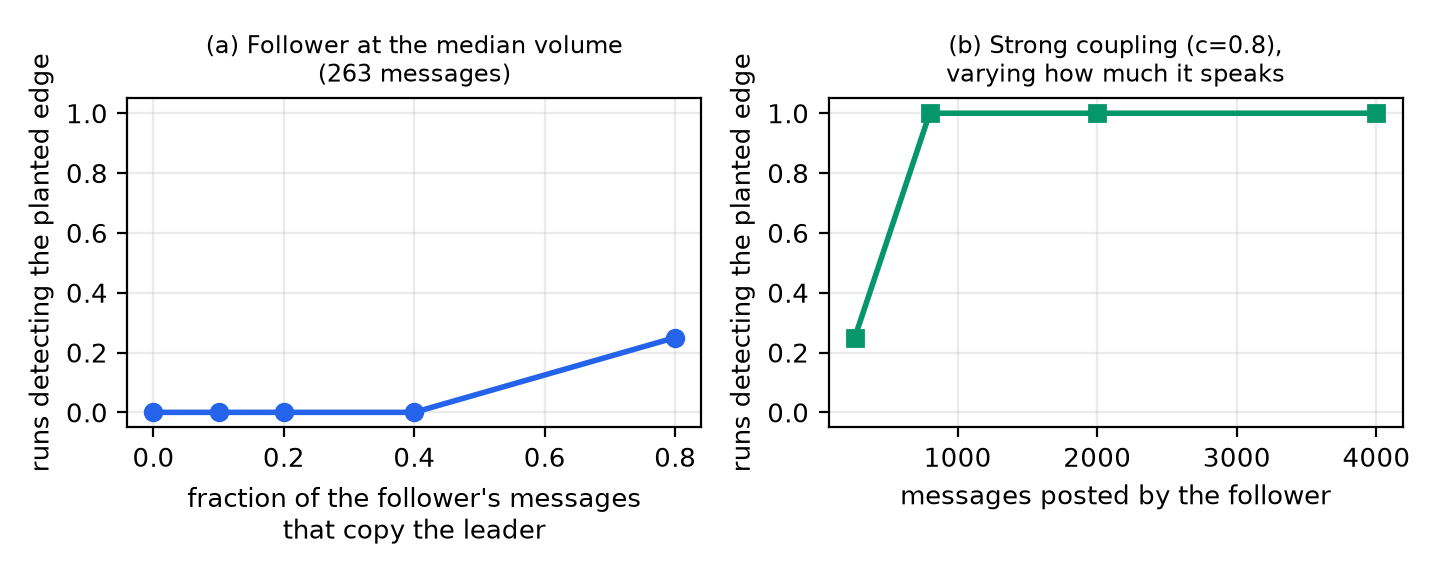
\includegraphics[width=0.92\textwidth]{f4_power.png}
\caption{Detection of a planted follower under the repaired surrogate. Left, varying the fraction of
its messages that copy the leader, at the median agent's volume. Right, varying how much it speaks,
at strong coupling.}
\end{figure}

\paragraph{Humans in the channel.} Main-village \#general is now effectively human-free, with 3 human
messages in the window, so the question has to be asked in open-chat, where 32\% of messages come
from 124 human visitors. Pairwise, with humans collapsed into one node, 19 edges are certified.
Conditioning removes almost all the agent-to-agent structure and little of the rest: \textbf{four
edges survive, of which three run from humans to agents, one is agent to agent, and none run from an
agent to a human.} The asymmetry is not an artifact of the confound. It should be read carefully all
the same: topical dependence from a person to an agent is also what ordinary responsiveness looks
like, so the measurement supports only that the dependence is dyad-specific and directional, not
that anyone is steering a swarm.

\section{Reproducibility, and one limitation of it}

Every number in this paper is recomputed from committed analysis output by a verifier that fails on a
mismatch, and that verifier covers the prose of this paper as well as the figures.

One limitation should be stated plainly. Re-running the counts in the earlier stationarity sweep with
the same seeds and configuration, only one of the eight cells reproduced exactly; the remaining
differences were one or two replicates per cell. Seven of the eight published rates still fell within
the recomputed Wilson intervals, and no conclusion changed. The exception is the zero-drift cell under
the permutation null, where the published 1 of 30 falls just below the recomputed interval of
$[0.035, 0.256]$ for 3 of 30, and no result here depends on that cell.

The generator, estimator and BLAS configuration were investigated and ruled out as the source. The
most likely explanation is a library-level difference, particularly in scikit-learn's $k$-means
implementation within the symboliser, whose output can vary between versions. Every sweep now records
the environment it ran under: Python 3.14.6, numpy 2.5.1, scipy 1.18.0 and scikit-learn 1.9.0,
including the BLAS build and the number of BLAS threads each worker used.

This does not make the previously published counts exactly reproducible. It provides a more clearly
specified environment in which subsequent results can be checked. For that reason I report rates
alongside their confidence intervals rather than exact replicate counts. The distinction between
reproducing a result within its uncertainty and reproducing every individual count matters, and only
the first is claimed.

\section{Conclusion}

Applied to real agent chat, the standard recipe for ``who drives whom'' needs repair before it says
anything. Clock windows cannot separate a message from its answer at the speed agents reply, and what
they certify is matched by a null with no access to meaning. The turn-ordered grid that fixes this
breaks the circular-shift surrogate: family-wise error 0.90 against a nominal 0.05, caused by the
speaker sequence itself. Restricted permutation surrogates repair most of that, but they are flat
under drift rather than calibrated, they are mutually indistinguishable at this precision, and one of
them needs twice the surrogate draws anyone would think to use. A valid surrogate fixes calibration
but not confounding. What survives is small: two dyad-specific edges that do not replicate, an
undetermined answer set by conditioning resolution, and influence running from people into agents and
never back. \textbf{An influence graph should not guide decisions until its error rate, its confound,
its detection floor and its symboliser's fidelity are reported.}

\section*{Limitations}

\begin{itemize}
\item \textbf{Immediate-predecessor only.} The turn-ordered lag-1 measure sees influence from the
message directly before a reply. Influence acting over several turns, or through a room's accumulated
context, is out of scope.
\item \textbf{Discrete approximation to an event process.} Agent chat is event-based in continuous
time. The turn-ordered discretisation with a permutation surrogate is a practical fix, and the
continuous-time comparison above shows what that choice gives up.
\item \textbf{The mechanism behind the real 0.90 is not established.} The generator separates
turn-taking from drift and points at drift, but the largest cell anywhere in the design is 0.365.
\item \textbf{Symbolisation quality cannot be measured on the real logs.} The central result survives
an independent symboliser, but the edge count does not: it moves with alphabet size and with which
messages the topic model is fit on. The floor remains the largest unquantified threat.
\item \textbf{No ground truth in the real logs.} The validity argument rests on planted controls and
on the meaning-free null, not on recovering a known answer.
\item \textbf{Conditioning removes real influence too.} The conditional estimate discards influence
that works by shifting what the channel is talking about, which in a group chat may be a large part
of genuine influence. It is a lower bound on dyadic influence.
\item \textbf{The human result is exploratory.} It rests on one village and one window and should be
read as a lead.
\end{itemize}

\section*{Broader impact and ethics}

This work audits influence detection on a population of AI agents, which is dual-use. Used
defensively it helps an overseer decide what an influence graph is worth, and the main result is
deflationary: it tells practitioners to trust these outputs less, which reduces rather than increases
the chance of acting on a bad attribution. The same tooling could be used to identify the most
influential agent in a swarm in order to target it, or to surveil participants in a channel. Three
properties limit the misuse. The subjects are AI models; the dataset is already public under research
terms and no re-identification is added; and the measure is weak and local, recovering
immediate-predecessor topical dependence rather than any model of how to steer an agent.

The dataset's research terms were followed: research use only, no training on the data, no
re-identification, citation of the source, and notification of the authors of resulting publications.
Human participants appear only as an aggregate node or as anonymised visitor labels, never by name or
handle, and no content attributable to an individual person is reported. Message text and metadata
were read, never model weights or private user data.

The use of a large language model in this work is disclosed in the first-page footnote, as TMLR
requires.

\bibliographystyle{tmlr}
\bibliography{refs}

\end{document}
"               de-anonymised arXiv preprint
%   pdflatex "\def\TMLRMODE{accepted}% TMLR submission. Built 10 November 2026 from:
%   paper/00_PROSE_v1.md   the author's written sections, 78 figures auto-verified
%   report/REPORT_V2.md    the sprint report, every number recomputed by report/verify_v2.py
%
% ANONYMITY. \usepackage{tmlr} with no option is the anonymous submission mode: the tmlr
% package hides the author block itself. Switching to [preprint] de-anonymises for arXiv AND
% turns on the \ifpreprint branches below, which are the only places a name, a repository URL
% or the benchmark's distinctive name appears. So one source produces both documents and the
% anonymous build cannot leak an identifier that the preprint build adds.
%
% Build:  latexmk -pdf main.tex
\documentclass[10pt]{article}

% The mode is chosen at build time so that one source produces every variant and they cannot
% drift apart:
%   latexmk -pdf main.tex                                        anonymous TMLR submission
%   pdflatex "\def\TMLRMODE{preprint}\input{main}"               de-anonymised arXiv preprint
%   pdflatex "\def\TMLRMODE{accepted}\input{main}"               camera-ready
% Use build.py, which runs all of them and checks the anonymous output for leaks.
\providecommand{\TMLRMODE}{submission}
\makeatletter
\def\@tmlrpreprint{preprint}
\def\@tmlraccepted{accepted}
\ifx\TMLRMODE\@tmlrpreprint
  \usepackage[preprint]{tmlr}
\else
  \ifx\TMLRMODE\@tmlraccepted
    \usepackage[accepted]{tmlr}
  \else
    \usepackage{tmlr}
  \fi
\fi
\makeatother

\usepackage{hyperref}
\usepackage{url}
\usepackage{booktabs}
\usepackage{graphicx}
\usepackage{amsmath}

% Gate every identifying string on whether identity may be revealed at all. The flag to test is
% \if@accepted, NOT \if@preprint: tmlr.sty's [preprint] option sets BOTH, so \if@accepted is true
% for the preprint and the camera-ready and false only for the anonymous submission, which is
% exactly the condition wanted. Gating on \if@preprint alone also hid the repository URLs from the
% camera-ready, which is where this paper promises to give them. \if@accepted is internal to
% tmlr.sty, hence the \makeatletter. The anonymous build takes the second argument.
\makeatletter
\newcommand{\ifdeanon}[2]{\if@accepted#1\else#2\fi}
\makeatother
\newcommand{\benchname}{\ifdeanon{SwarmInfluence-Bench}{the benchmark}}

% An unmarked footnote, for the LLM-use disclosure. TMLR's FAQ requires the disclosure and names
% the location: authors must "mention explicitly in their submission that they have used this
% tool", "as a footnote on the first page". Verified against jmlr.org/tmlr/faq.html on 10 Nov 2026.
% It is therefore not optional, and it does not belong in Broader Impact, where it sat until now.
% Nothing in the policy asks for the vendor's name, so none is given.
\newcommand{\disclosurefootnote}[1]{%
  \begingroup\renewcommand\thefootnote{}\footnote{#1}\addtocounter{footnote}{-1}\endgroup}

\title{An Influence Graph Over AI Agents Certifies an Agent That Copies Nobody}

% Hidden by the tmlr package unless [accepted] or [preprint] is given.
\author{\name Manu Nicholas Jacob \email manunicholasjacob@gmail.com \\
        \addr Independent Researcher}

\def\month{11}
\def\year{2026}
\def\openreview{\url{https://openreview.net/forum?id=XXXXXXXXXX}}

\begin{document}
\maketitle

\begin{abstract}
Circular-shift surrogates can produce severely inflated false-positive rates when applied to
turn-ordered multi-agent conversations, reaching a family-wise error rate of 0.90 against a nominal
0.05. A generated benchmark separates two candidate mechanisms and points at non-stationary speaker
activity rather than turn-taking, which suppresses the failure rather than causing it. No setting of
either knob reproduces the observed 0.90, however, so what drives the full real-data failure remains
open. Restricted permutation surrogates substantially reduce the problem. Their error rate is flat
with respect to drift rather than at the nominal level, and for the global within-speaker variant it
depends on how many surrogate draws the null is built from. Calibration alone does not address
confounding, which motivates a conditional estimator validated against a benchmark with planted
ground truth. I also identify a symbolisation-dependent detection limit and develop label-free
diagnostics for it, and show that their calibration does not transport across degradation
mechanisms. The benchmark is released.
\end{abstract}

\disclosurefootnote{\textbf{Use of a large language model.} A large language model was used as an
assistive tool: to help write and run the analysis code, and to help draft this paper. The author is
responsible for every claim, number and figure. All results come from the released code run on the
public dataset, no result or reference is fabricated, and every number in this paper is recomputed
from committed analysis output by a verifier that fails the build on a mismatch.}

\section{Introduction}

When AI agents interact in a shared channel, it is useful to understand how they influence one
another. Information-theoretic methods offer a way to measure this through lagged transfer entropy,
surrogate testing, and per-agent influence scores. They are attractive because they require no
labels and no access to model internals, only a record of who said what and when. The reliability of
those measurements is what this paper examines.

Almost every demonstration of these detectors runs on synthetic traces with a planted leader, where
the analyst controls timing and vocabulary. Real agent chat is asynchronous, bursty, and written in
open language. The narrower question here is whether the standard recipe, applied to real agent
logs, returns anything an overseer should act on.

The audit runs on the AI Village corpus \citep{aidigest2026}, in which frontier models share chat
channels over eighteen months across four villages differing in size, lifetime and tempo, applying
the checks a reader should demand: planted controls, a meaning-free symboliser, replication in a
held-out window, and sensitivity to every parameter that had to be chosen.

\begin{enumerate}
\item The conventional circular-shift surrogate is \textbf{invalid} on turn-ordered agent chat: a
family-wise error rate of 0.90 against a nominal 0.05, caused by the structure of the speaker
sequence itself.
\item Restricted permutation surrogates restore most of the calibration, and re-certifying under one
\textbf{scrambles rather than shrinks} the answer: one channel loses all 11 of its edges, another
gains 15.
\item The three restricted variants are \textbf{mutually indistinguishable} at the precision reached
here, so the choice between them cannot be justified on error rate. The global within-speaker
variant additionally needs on the order of 200 surrogate draws, and over-fires by roughly a factor
of two at 100.
\item Calibration is not confounding, so a conditional estimate is added and validated on a released
benchmark with a known influence graph: common-cause false edges fall from 22.3 to 0.33, and on the
planted-edge instances precision rises from 0.17 to 0.80 with no loss of recall or power.
\item The same benchmark exposes a \textbf{symbolisation floor}. Below roughly 0.44 adjusted Rand
index between symboliser and truth, detection collapses whatever the estimator. Label-free
diagnostics detect that floor, but their calibration does not transport across degradation
mechanisms, and I report where it fails.
\item On the real channels two edges stand at every conditioning resolution, 18 are
\textbf{undetermined} between 0 and 13, none replicates out of sample, and what survives alongside
humans runs from people to agents.
\end{enumerate}

\section{Related work}

\paragraph{Transfer entropy and surrogates.} Transfer entropy \citep{schreiber2000} measures how much
a source's past reduces uncertainty about a target's next symbol beyond the target's own past.
Plug-in estimators are biased upward on short series, so significance rests on surrogate data, with
family-wise error controlled by a max-T test \citep{westfall1993}. The usual surrogate is a circular
time shift of the source.

\paragraph{Event-based data breaks the shift surrogate.} \citet{shorten2021}, on neural spike trains,
show that the conventional source-time-shift surrogate fails to represent the null hypothesis of
conditional independence for event-based processes, and adapt to that setting the nearest-neighbour
local permutation scheme of \citet{runge2018}. Agent chat is event-based in that sense: messages are
events in continuous time, not samples of a clocked signal. The correction is not a contribution of
this paper. The contribution is showing that the same failure carries over to multi-agent safety
monitoring, and that it can be severe enough to create apparent leaders where none exist.

\paragraph{The same failure, concurrently, in multi-agent reinforcement learning.}
\citet{papadopoulos2026} report a closely related surrogate failure in multi-agent
reinforcement-learning action series. Their agent pairs have zero influence by construction, yet
circular time shifts produce false-positive rates of 100\% and 98.2\% against a nominal 0.05. A
plain permutation surrogate fares no better in their setting, at 100.00\% and 99.95\%. Their
proposed correction restricts permutations to blocks of training time, which returns the rates to
5.25\% and 5.50\%.

There are important differences between their setting and this one. Their data consist of binary
actions recorded over twelve thousand training rounds, whereas these data are symbolised
natural-language messages arranged on a turn-ordered conversational grid. Their non-stationarity
comes from monotone drift associated with annealing exploration; here the relevant non-stationarity
appears in the speaker sequence. Neither result should be taken as a direct extension of the other.

Nevertheless, the fact that both approaches rely on restricted permutations is worth noting. Their
permutation blocks are defined by training time, while mine are defined by an agent's own speaking
positions. This provides convergent evidence that unrestricted temporal rearrangement can be
problematic in non-stationary multi-agent data. Their findings also serve as a useful warning for
the approach taken here, and the warning has a measured form rather than a rhetorical one: in their
data the unrestricted permutation failed as completely as the time shift, at 100.00\% against a
nominal 0.05. Permutation-based surrogates are not automatically protected against
non-stationarity, and what protects the one used here is the restriction, not the permutation. I
claim no priority over their result and view the two studies as complementary, addressing different
forms of structured multi-agent data.

\paragraph{Oversight under a budget.} AI-control research frames monitoring as resource constrained,
with a cost for false positives \citep{greenblatt2024}. An influence graph is one such measurement,
and its error rate is the concern here.

\paragraph{Clustering stability.} The idea of using clustering stability as a label-free quality
indicator is not new. It has a substantial history, including \citet{benhur2002},
\citet{lange2004}, von Luxburg's review of clustering stability \citep{vonluxburg2010}, and
\citet{tibshirani2005} on prediction strength. What is different in Section~\ref{sec:floor} is the
calibration of these diagnostics against a detection-performance floor rather than against cluster
recovery alone.

\section{Data and representation}

The AI Village dataset ships one gzipped-JSONL table per village. Four villages are used, differing
enough to test whether any finding is a property of one channel.

\begin{table}[h]
\centering
\begin{tabular}{lrrrrl}
\toprule
village & agent messages & agents & lifetime & human messages & busiest room \\
\midrule
main      & 205,726 & 58  & 576 days & 10,029 & \#general (166,715, 81\%) \\
open-chat &  35,483 & 23  &  66 days & 12,264 & \#general (all) \\
swarm     &   3,848 & 133 &   1 day  &      5 & room a (3,846) \\
game-jam  &     838 & 6   &   3 days &     36 & per-team rooms \\
\bottomrule
\end{tabular}
\caption{The four villages. A 2026 scaffolding change scopes each agent to its current room's
context, so the busiest room of each village is a self-contained influence substrate and is analysed
alone.}
\end{table}

The primary window is the final fourteen days of main-village \#general, 17 to 31 October 2026,
holding 8,800 agent messages. Twenty-two models posted at least 50 messages each and the directed
test uses the 15 busiest, giving 7,958 message events. Two scaffolding facts are disclosed rather
than corrected: the automated nudger was off throughout, and the unused \#best and \#rest rooms were
soft-deleted mid-window, which does not touch \#general.

\subsection{From open language to symbols}

Transfer entropy needs discrete symbols, so each message is mapped to a small alphabet before
influence is estimated, and that mapping is kept separate from the estimator. A topic symboliser
(TF-IDF then $k$-means, $k=8$) gives a message its topic cluster id, so paraphrases of one idea share
a symbol. A hash symboliser, a stable hash of the normalised text into $k=8$ buckets, has no notion
of meaning and serves as a null: an edge appearing under both lives in timing alone.

\subsection{The lag problem, and why clock windows cannot solve it}

A lag-1 transfer entropy compares window $t-1$ with window $t$, so influence landing inside one
window is invisible to it. Agent chat makes this binding. Among the fifteen analysed agents the gap
between consecutive messages by different speakers has a median of 28.1 seconds (25th percentile
9.2, 75th 66.2, 95th 159.3), so turn-taking is a seconds-scale process while any clock window wide
enough to hold two speakers is minutes wide and swallows both a message and its answer.

Both horns are measurable. At 30 seconds only 1.2\% of agent-windows hold a message, while 32.0\% of
replies already land in the same window as what they answer, rising to 84.4\% at five minutes. At
every width tried, the meaning-free hash null certifies comparably many edges, and more at five
minutes: 9 against 12 at thirty seconds, 17 against 19 at one minute, 27 against 44 at fifteen, and
19 against 17 at five. Whatever clock-window transfer entropy was detecting there, it was not shared
meaning.

\begin{figure}[h]
\centering
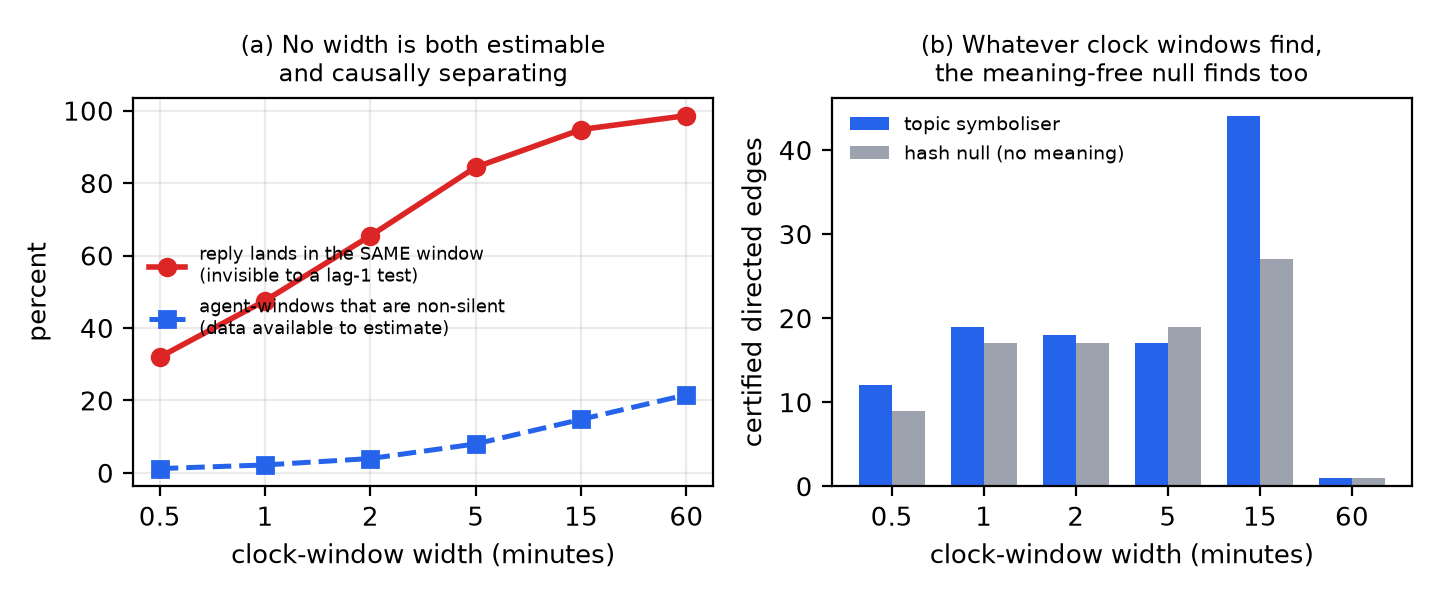
\includegraphics[width=0.92\textwidth]{f1_clock.png}
\caption{Clock-window transfer entropy on the 15 analysed agents of main-village \#general. Left,
the two failure modes as a function of window width. Right, edges certified under the topic
symboliser against the meaning-free hash null.}
\end{figure}

The bind is avoided by ordering messages canonically and letting one message be one tick. Each
agent's series carries its symbol where it spoke and a silent symbol elsewhere, so the lag-1
comparison is between a message and the one immediately before it. The cost is that the measure
captures immediate-predecessor influence only.

\section{The surrogate failure, and two explanations that did not hold}
\label{sec:failure}

An agent is planted into the real stream, drawing its symbols from the channel's marginal and
coupled to nothing at all. It is certified as driving something in 3 of 8 runs when it posts 50
messages, and in 8 of 8 at 100, 263, 600 and 1500 messages, with the mean largest $z$ rising from 5.6
to 12.3, 21.7, 38.3 and 71.7. The error grows with how much the agent speaks, which rules out a
small-sample explanation.

A planted agent could be dismissed as artificial, so the error rate is also measured directly.
Keeping the real speaker sequence and permuting the symbols globally leaves data with no directed
topical influence by construction. The shift surrogate certifies at least one edge in 9 of 10 such
replicates, a family-wise error rate of 0.90 against a nominal 0.05.

\paragraph{What breaks it is the speaker sequence.} Destroying one structure at a time isolates the
cause. Keeping the real speaker order and shuffling only symbols, the shift surrogate fires in 10 of
10 replicates; randomising the speaker order as well drops it to 0 of 10; uniform symbols with the
real order still give 6 of 10. So the driver is the structure of the speaker sequence, not the
symbol distribution and not sparsity. That sequence is far from random in two ways at once: it
repeats a speaker 36\% of the time and returns after one message 38\% of the time, and each agent's
activity is strongly non-stationary, with a median block-share coefficient of variation of 0.79.
Shuffling the order destroys both at once, so this ablation cannot say which of the two mattered.

\subsection{Two explanations I proposed, and the benchmark refuted both}

I initially attributed the failure to mutual exclusivity: only one agent can speak at each tick, so
shifting individual timelines could create overlaps that never occurred in the original
conversation. The benchmark did not support this explanation. A generated channel with exactly one
speaker per tick and steady activity produced an error rate of just 0.025, 95\% Wilson
$[0.011, 0.057]$, far below the 0.90 observed in the real data. Mutual exclusivity alone therefore
cannot explain the failure.

I then suspected turn-taking. In the real channel, speakers repeat 36\% of the time and return after
exactly one message 38\% of the time. However, adding a Markov speaker chain to the generator
produced the opposite result. Turn-taking suppressed the error rather than increasing it. At the
nominal knob values and with no drift the surrogate certified nothing at all across 200 replicates,
while removing turn-taking and introducing drift raised the rate to 0.365. The contribution from
drift was $+0.340$, compared with $-0.025$ for turn-taking. The same inversion appears in the arm
calibrated so that the generated channel reproduces the real channel's measured repeat, return and
block-share statistics rather than merely carrying those numbers as settings: there, turn-taking
alone also certifies nothing, and drift alone gives 0.065.

Neither mechanism, nor their combination in the tested design, reproduced the real-data error rate of
0.90. The largest cell anywhere in the design is 0.365. The real-data ablation removes turn-taking
and non-stationarity together, while the generator separates them. The results point to
non-stationary activity, but the remaining gap means the mechanism behind the full real-data failure
is not yet established.

Every figure above comes from the run at 200 surrogate draws. The first version of this analysis
used 100, which inflates both nulls on the same 2,400 instances: the circular shift fires 53 times
where the 200-draw run does not, against 18 the other way (exact McNemar $p = 3.9 \times 10^{-5}$),
and the permutation surrogate 83 against 20 ($p = 2.7 \times 10^{-10}$). Every qualitative conclusion
in this section is the same at both settings, which is why they are worth stating at all. The
numbers are not, so the draw count belongs in the caption.

\section{The repair, compared}
\label{sec:repair}

Following the local-permutation idea of \citet{runge2018} as adapted by \citet{shorten2021}, each
source keeps its speaking positions and only its symbols are permuted among them. Speaking pattern,
sparsity and turn-taking are preserved exactly, and only the correspondence between symbol and time
is destroyed. On the same destroyed-structure real data the family-wise error rate falls to 0.063
over 300 replicates, 95\% Wilson $[0.041, 0.097]$. The planted uncoupled agent is never certified: 0
of 5 at both 263 and 1500 messages, with mean max $z$ of 2.8 in each case against 22.0 and 68.3
under the shift surrogate.

\begin{figure}[h]
\centering
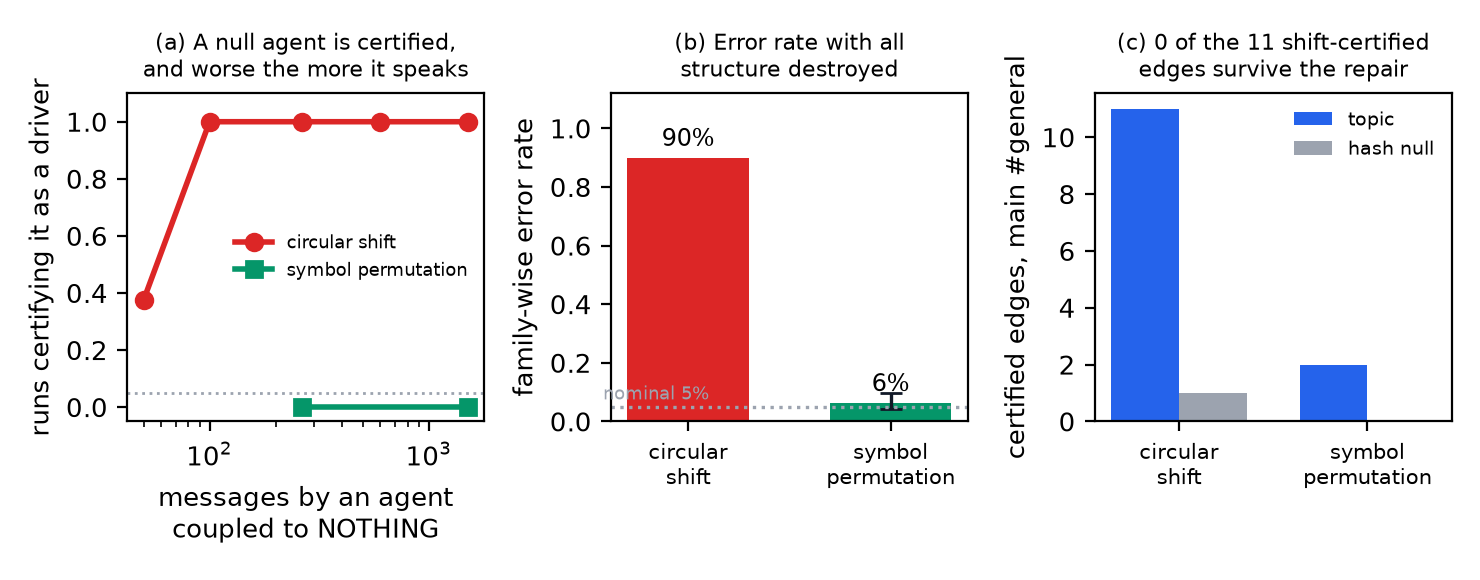
\includegraphics[width=\textwidth]{f2_null.png}
\caption{Left, how often an agent coupled to nothing is certified as a driver, under each surrogate.
Middle, family-wise error rate measured on data with all structure destroyed, with a Wilson
interval; the dotted line is the nominal 0.05. Right, what each surrogate certifies on the real
channel.}
\end{figure}

\subsection{How many surrogate draws are needed}

The number of surrogate draws matters more than I initially appreciated. In a paired comparison of
300 instances, where all four surrogates run on identical symbol grids so the outcomes are paired,
the global permutation surrogate produced a false-positive rate of 0.1167 with 100 draws, falling to
0.0700 with 200 draws, 95\% Wilson $[0.046, 0.105]$. This difference is statistically significant
(exact McNemar $p = 0.0043$). The block-local and Runge local permutations were less sensitive to the
increase: their corresponding rates changed from 0.0900 to 0.0767 and from 0.0967 to 0.0800.

At 200 draws, the global permutation's interval covers the nominal 0.05 and overlaps the real-data
estimate of 0.0633 $[0.0409, 0.0968]$. The real-data result is therefore corroborated rather than
overstated. For practical use, the important point is that reducing the number of surrogate draws
can materially change the result. In particular, the global permutation over-fires at 100 draws by
approximately a factor of two. I would therefore not treat the choice of draw count as a minor
computational detail.

The same correction applies to the benchmark-wide estimate. That figure was 0.0942 at 100 draws.
Repeating all 2,400 instances at 200 draws gives \textbf{0.0679}, 95\% Wilson $[0.0585, 0.0787]$,
and the paired difference is large: 83 instances fire at 100 draws and not at 200, against 20 the
other way, $p = 2.7 \times 10^{-10}$. The conclusion it supports is unchanged, because the interval
still excludes the nominal 0.05. So the permutation repair does carry a residual inflation on clean
generated data, but it is about a third above nominal rather than nearly double.

One limit on this recommendation. I compared 100 draws against 200 and did not test any larger
value, so what the experiment establishes is that 100 is too few, not that 200 is enough. Two
hundred is a lower bound on the draw count rather than a converged setting, and a practitioner whose
conclusions sit near a decision boundary should check their own sensitivity rather than adopt the
number.

\subsection{Choosing a repair, when the error rate cannot choose}

The comparison of the three permutation-based repairs does not produce a clear winner. All four
surrogates were evaluated on identical symbol grids across 300 pure-null replicates, so the
comparison reflects differences between the null models rather than differences between datasets.

\begin{table}[h]
\centering
\begin{tabular}{lrrrl}
\toprule
surrogate & FWER, 100 draws & FWER, 200 draws & 95\% Wilson at 200 & nominal 0.05 \\
\midrule
circular shift                   & 0.0433 & \textbf{0.0333} & $[0.018, 0.060]$ & inside \\
global within-speaker permutation & 0.1167 & \textbf{0.0700} & $[0.046, 0.105]$ & inside \\
block-local permutation          & 0.0900 & \textbf{0.0767} & $[0.052, 0.112]$ & excluded \\
local permutation \citep{runge2018} & 0.0967 & \textbf{0.0800} & $[0.054, 0.116]$ & excluded \\
\bottomrule
\end{tabular}
\caption{Four surrogates on identical symbol grids, 300 pure-null replicates, at both draw counts.}
\end{table}

At 200 draws, paired on the same 300 instances, the circular shift is not significantly different
from the global permutation ($p = 0.0614$), although it differs from block-local permutation
($p = 0.0294$) and from Runge's local permutation ($p = 0.0201$). At 100 draws it differed from all
three, which is the draw-count artifact again. The three repairs remain statistically
indistinguishable from one another, with pairwise $p$-values of 0.85, 0.65 and 1.00. The apparent
differences in their error rates are not sufficient to establish a ranking.

Choosing between them therefore requires more than calibration, and two readings pull against each
other. Runge's local permutation has the strongest methodological justification for preserving the
structure it is intended to preserve, and it follows the approach adapted to event data by
\citet{shorten2021}. Block-local permutation is more heuristic and introduces a free parameter that
has not been tuned. Global permutation is the simplest. On the other hand, the global permutation has
the most favourable interval relative to the nominal rate, and is the only repair that costs nothing
measurable against the shift on clean stationary data, although neither difference is statistically
established. I do not consider the observed error rates sufficient to select one repair over the
others. The choice should be guided by the structure the null is intended to preserve and the
assumptions that can be justified for the data.

\subsection{When to use the repair}

A drift sweep gives the practical reading. Across 150 replicates per cell at 200 surrogate draws,
the circular shift degrades steadily as activity drift increases while the three repairs do not.

\begin{table}[h]
\centering
\begin{tabular}{lrrrr}
\toprule
activity drift & circular shift & global permutation & block-local & local \\
\midrule
0.0 & \textbf{0.013} & 0.093 & 0.080 & 0.093 \\
0.3 & 0.100 & 0.100 & 0.093 & 0.120 \\
0.6 & \textbf{0.193} & 0.053 & 0.047 & 0.067 \\
0.9 & \textbf{0.380} & 0.087 & 0.080 & 0.080 \\
\bottomrule
\end{tabular}
\caption{Family-wise error on pure nulls as activity drift increases, 150 replicates per cell, 200
surrogate draws. Every certified edge is a false positive by construction.}
\end{table}

The pattern is supported by a formal trend test rather than by eye. A Cochran-Armitage test across
the four ordered drift levels gives the circular shift $z = 8.667$, $p < 10^{-15}$, and gives every
repair nothing: $p = 0.51$ for the global permutation, 0.63 for block-local and 0.37 for local. The
same pattern holds at both surrogate draw counts, so it does not depend on that choice.

The repairs are therefore flat under drift rather than calibrated. Only one of the four global
permutation intervals covers the nominal 0.05, and the rest sit nearer 0.09, so what the repair buys
is insensitivity to drift rather than correctness. One asymmetry should be stated rather than
hidden: block-local covers nominal in three of the four cells where the global repair covers one.
The two remain pairwise indistinguishable, so this is not grounds to switch the recommendation, but
it does mean the global repair cannot be described as the best-calibrated under drift.

The results also show why the repair should not be treated as universally preferable. At zero drift
the circular shift has an error rate of 0.013, while the three repairs are all around 0.08 to 0.09.
That advantage is gone by the first drift step: at drift 0.3 the shift reads 0.100 against the global
permutation's 0.100 and block-local's 0.093, so the crossover falls between drift 0.0 and 0.3 rather
than at some higher level. By drift 0.6 the shift is roughly four times the repairs. If a channel has
been checked and found stationary, the circular shift may be sufficient. When activity is
non-stationary the repairs are the more stable choice, and the margin for error on that judgement is
narrow, because the crossover arrives by the first drift level tested.

\section{Continuous time, and what the repair cannot test}

An earlier analysis identified continuous-time estimation as the principled option for event data
but did not evaluate it. Running the continuous-time estimator CoTETE on both channels certifies 0
edges in either case, compared with 2 for main-village and 18 for open-chat under the discrete,
turn-ordered analysis. Its highest $z$-scores are 3.062 and 3.980, below the respective max-T
thresholds of 4.171 and 4.308.

At first these results might appear to contradict the symbol-based analysis. The two estimators
operate on different information, however. CoTETE's public API takes event times with no symbol
channel, while the transfer-entropy analysis here uses topic symbols. To test whether this
difference explains the results, I reduced the data to timing alone, replacing every spoken symbol
with the same code. Under this representation the estimator used here also detects 0 edges in both
channels, matching CoTETE. Using the circular-shift surrogate instead produces 12 and 3 edges. So
neither method detects relationships from event timing alone in these channels, and the edges found
by the symbol-based analysis depend on symbol correspondence, which the continuous-time estimator
cannot access.

Two caveats attach to those $z$-scores, and the second attaches to the larger of them. Point
estimates from this estimator are stochastic to about 17\% across repeated runs, so none of these
values should be read to more than two significant figures. And open-chat's highest $z$, the 3.980,
belongs to the one pair whose surrogate draws mostly failed: it needed 1,936 failed draws to obtain
100 successes, a 4.9\% success rate. Those surrogates are conditioned on being estimable, so that
pair's null is biased in an unknown direction. The conclusion does not rest on it, since that pair
falls below threshold and so does every other pair, but the number should not be quoted as a clean
measurement. The failures themselves were a defect rather than a property of the data: an enlarged
exclusion window can empty the neighbour search on sparse bursty event trains and raise an error
that terminates a whole pair, with no handling at the public entry point. This has been reported
upstream.

There is also a fundamental limitation in applying the recommended permutation surrogate to
timing-only data. When every event carries the same symbol, permuting those symbols changes nothing.
The observed statistic and the surrogate null are identical, making the test exactly degenerate:
standard deviation 0 across all 210 pairs and $p = 1.0$ everywhere. \textbf{The repair has zero power
against timing structure by construction.} The permutation surrogate is appropriate for testing
relationships in the symbol sequence, but it does not answer whether relationships exist in event
timing. These are different questions, and choosing one null means giving up the ability to test the
other with that procedure.

\section{Confounding, and what conditioning removes}

A valid surrogate fixes calibration but not confounding. If every agent tracks a drifting channel
topic, every pair is genuinely dependent through the channel, and pairwise transfer entropy cannot
tell that from direct influence. I therefore also report a \textbf{conditional} estimate, which asks
whether a source's last message adds anything about a target's next one beyond the target's own
history and the channel's recent state. The conditioning variable is the modal symbol of the last
twelve messages, excluding the immediately preceding one so that it does not simply restate the
source.

On a generated benchmark whose decisive instances contain no influence while every agent tracks a
shared drifting topic, so that any certified edge is common cause, pairwise transfer entropy
certifies \textbf{22.3} edges on average and conditioning takes that to \textbf{0.33}, lifting pooled
precision on the four-edge instances from 0.17 to \textbf{0.80} at a recall of 1.0 either way. Across
couplings from 0.05 to 0.8 the conditional test still finds the planted edge in 3 of 3 runs, so the
gain costs no power.

The benchmark flatters the conditional estimator, since its common cause is a shared modal topic and
the conditioning variable is the channel's modal topic. The real channels are harder, and
conditioning there costs degrees of freedom: a 9-symbol alphabet with a 9-valued context gives 6,561
cells against about 7,900 ticks, so that variable is also coarsened to 4 and 2 values.

\begin{table}[h]
\centering
\begin{tabular}{lrrrr}
\toprule
channel & pairwise & conditional, 9 values & 4 values & 2 values \\
\midrule
main \#general      & 2  & \textbf{2, the same two edges} & 2 & 3 \\
open-chat \#general & 18 & \textbf{0} & \textbf{7} & \textbf{13} \\
swarm, room a       & 1  & \textbf{0} & & \\
\bottomrule
\end{tabular}
\caption{Conditioning at three resolutions. Main-village's two edges are robust to that choice;
open-chat's zero is not.}
\end{table}

At the finest resolution the open-chat test is degenerate, its surrogate sitting above the observed
statistic for 65\% of pairs with the largest $z$ in the family only 4.4, so it is failing to reject
rather than finding nothing to reject. Open-chat's structure therefore remains
\textbf{undetermined}: depending on the conditioning resolution, between 0 and 13 of its 18 edges may
survive. That resolution is a free parameter an analyst would set once and never revisit. This is a
property of the channel rather than the estimator: on structure-free real data the conditional test
fires in 2 of 40 replicates, an error rate of 0.05 with a mean $z$ of $-0.001$, so it is nominal
rather than conservative.

\section{The symbolisation floor}
\label{sec:floor}

Everything these methods produce is downstream of turning text into symbols. On the benchmark, where
the underlying topics are known, detection performance drops sharply when agreement between the
symboliser and the ground truth falls below roughly ARI 0.44, and this behaviour appears across the
tested estimators. Importantly, the false-positive rate can look \emph{better} below this point,
because the shared topic structure needed to produce confounded detections is no longer represented
reliably. A pipeline that stops detecting relationships may therefore have lost the signal it needs
rather than become more reliable, and nothing downstream of the symboliser can tell those apart.

\subsection{Detecting the floor without labels}

That degradation can be detected without ground-truth labels. Across the nine-level benchmark sweep,
three statistics separate the below-floor cases with zero errors: seed stability at a threshold of
0.623, agreement with LSA at 0.646, and the Calinski-Harabasz index at 138.9. Seed stability here is
the \textbf{minimum} pairwise agreement across seeds, not the mean; the mean variant makes one error,
at a different threshold of 0.791. Silhouette has the strongest correlation with true ARI, at 0.979,
but is not useful for identifying the boundary because its threshold falls within a gap of just
0.002. A statistic that tracks clustering quality most closely is not necessarily the best one for
making a classification decision.

Error count cannot choose among the three that were perfect, so I tested whether each threshold still
means what it meant when the channel changes for reasons other than topic separability. Applying each
cut unchanged to thirty cells that vary turn-taking, drift, agent count, volume skew, message length
and corpus size, twenty-seven of which hold true ARI at exactly 1.000:

\begin{table}[h]
\centering
\begin{tabular}{lrrrr}
\toprule
diagnostic & cut & errors where fitted & errors, nuisance set & of those at true ARI 1.000 \\
\midrule
seed stability, min across seeds & 0.623 & 0 & 2 & \textbf{0} \\
LSA agreement                    & 0.646 & 0 & 2 & \textbf{0} \\
Calinski-Harabasz                & 138.9 & 0 & 6 & \textbf{3} \\
\bottomrule
\end{tabular}
\caption{Whether a cut fitted on the vocabulary-overlap mechanism survives a change in the channel
that is not a change in topic separability.}
\end{table}

The two bounded statistics err only on the short-message cells, where the symbolisation genuinely has
degraded. Calinski-Harabasz additionally condemns all three cells whose true ARI is exactly 1.000,
for no reason beyond the corpus holding 2,000 messages rather than 8,000, where it reads 76 to 77
against its own cut of 138.9. It is unbounded and grows with sample size, so a published numeric
threshold for it carries no meaning on another corpus. That is why I recommend the two bounded
statistics and not the index that matched them on error count. \textbf{A cut that moves with the
corpus is not a floor cut.}

This is not a weak statistic being discarded on a technicality. Calinski-Harabasz correlates with
true ARI at 0.973, almost as closely as silhouette, and unlike silhouette it classifies the floor
perfectly where it was fitted. It still cannot carry a published threshold. That is the sharper form
of the point above: neither the statistic that tracks quality most closely nor the one that
classifies best on the fitting mechanism is necessarily the one whose cut another researcher can
reuse.

There are important limits to this result. The effective sample size is nine rather than 54, because
the classification label is determined by overlap level. There are no observations between ARI 0.444
and 0.222, so the exact location of the boundary within that interval remains unknown. These
diagnostics classify whether a result is below the tested detection floor; they do not estimate ARI,
and their behaviour is flat between 0.68 and 1.00, and not even monotone there. The benchmark also
uses a single degradation mechanism with a known and correct value of $k$, whereas the true number of
topics in real conversations is unknown. I therefore treat 0.44 as a benchmark-specific, bracketed
result rather than a universal threshold.

\subsection{A contradiction the diagnostic lost}

I initially used these diagnostics to classify one real channel, open-chat, as below the
symbolisation floor. That conclusion did not agree with the channel's measured results: open-chat
certified 18 and 22 edges under the two symbolisers, compared with 2 and 1 for main-village, and its
hash-based null certified zero edges. Rather than treating this disagreement as evidence that the
original measurements were wrong, I revisited the diagnostic itself.

The problem was the choice of $k$. Repeating the comparison with the same channels, loader and window
reproduced the published $k=8$ results to the digit. At $k=4$, however, open-chat reached stability
scores of 0.950 and 0.978, the highest values produced by either channel across the tested settings,
and both exceeded the diagnostic thresholds. The earlier below-floor classification was therefore a
conclusion about one arbitrary choice of $k$, not a reliable statement about the channel. Message
length does not explain the difference either: 27.1\% of main-village messages contain fewer than
five tokens, compared with 2.3\% in open-chat, so the short-message channel is the one the diagnostic
cleared.

This correction changes how the symbolisation results should be read, and it withdrew three claims.

\begin{enumerate}
\item \textbf{The claim that no topic signal remains below the floor is too strong.} The
circular-shift surrogate recovers all four planted edges at every tested overlap level, including
0.95, where ARI is 0.011. The observed collapse is in the permutation null, not necessarily in the
underlying data.
\item \textbf{ARI 0.44 cannot be treated as a universal detection threshold.} When the shared-topic
parameter is 0, detection continues down to ARI 0.296, so the boundary depends on both the
symboliser and the channel.
\item \textbf{Edge counts cannot be used as a measure of symboliser quality.} Even at ARI exactly
1.000, changing the shared-topic parameter alone moves the permutation edge count from 5 to 78.
\end{enumerate}

The diagnostics also do not transfer reliably outside the mechanism on which they were evaluated.
Their balanced accuracy falls from 1.00 to 0.75 and 0.571 under a known mismatch in $k$. All seven
errors made by seed stability are false below-floor classifications, and in every one of those cases
the detector still identifies all planted edges; of the fourteen cells it condemned, eleven had full
conditional recall. The failure direction is the dangerous one: it condemns working symbolisations.

This was an important correction to my own interpretation. I introduced a diagnostic to check whether
the symbolisation was reliable, applied it to the real channels, and found that it contradicted
measurements already in hand. Investigating that contradiction showed the diagnostic was sensitive to
an arbitrary modelling choice. The result is not that the original measurements were wrong, but that
the control was being asked to support a broader conclusion than the evidence allowed. These
diagnostics remain useful within their tested setting, and \textbf{no channel-level floor verdict
should be issued from a single $k$}.

\section{The benchmark}

Real logs have no ground truth, so the common-cause question could not be settled on them. The
generator used here makes the influence graph known by construction: it decides, in code, who speaks
at which tick, on which topic, and who reacts to whom. Surface text is a separate, replaceable layer
drawn from disjoint per-topic vocabularies, so the whole thing runs offline and a detector still has
to symbolise raw text rather than read the labels. Turn-taking and activity drift are independent
knobs, so the two can be varied one at a time, and the generator reproduces its earlier behaviour
bit for bit when both are zero.

\benchname{} is released with 150 tests covering the generator, the detector harness, the text layer,
the floor analysis and the turn-taking factorial.
\ifdeanon{Code and benchmark:
\url{https://github.com/manunicholasjacob/swarm-influence-bench} and
\url{https://github.com/manunicholasjacob/swarm-influence-audit}.}{Code and benchmark are publicly
released; the links are withheld here for anonymity and will be given in the camera-ready version.}

One property of the benchmark must be stated when its numbers are quoted. Planting an edge displaces
other agents' speaking turns, so the generated instances contain real lag-1 dependencies that the
label set does not list. Precision measured against those labels is therefore a \textbf{lower bound}
for any detector, and what the benchmark supports is the comparison between two estimators rather
than the absolute value of either.

\section{What an overseer should do}

Six inexpensive controls should be included whenever an influence graph over an agent channel is
published.

\begin{enumerate}
\item \textbf{Plant an agent coupled to nothing, at your channel's volumes, and check it is not
certified.} This one test would have caught the failure reported here, at one run per volume.
\item \textbf{Measure the error rate directly}, by destroying the structure your method claims to
find and checking the family-wise rate is near nominal. If it is not, your surrogate does not match
your data.
\item \textbf{Preserve the speaker sequence in your surrogate.} Any surrogate that moves an agent's
messages in time will disturb it, and \citet{shorten2021} is the principled route. Use at least 200
surrogate draws, because at 100 the global within-speaker permutation over-fires by roughly a factor
of two.
\item \textbf{Establish the detection floor before interpreting an absence.} ``No edges'' and ``no
influence'' are different claims.
\item \textbf{Condition on the channel, report both numbers, and sweep the resolution.} Pairwise and
conditional bound the answer, and the gap between them is the result. Conditioning costs cells, so
check whether your answer is an artifact of how finely you conditioned. On one channel here it was.
\item \textbf{Report how well your symboliser agrees with the truth, on data where you know it.}
Everything is downstream of turning text into symbols, and below roughly ARI 0.44 detection
collapses whatever the estimator. I have found this control in no influence-detection paper, and it
is also the one that cannot be run on real logs, which is why the floor remains the largest
unquantified threat here.
\end{enumerate}

Two habits follow: publish a meaning-free null's count beside the real one, and require held-out
replication before calling a graph a structure.

\section{The real channels, and what survives}

Re-running every channel under the repaired surrogate changes the answers, and not in one direction.

\begin{table}[h]
\centering
\begin{tabular}{lrrr}
\toprule
channel & window messages & shift: topic / hash & permutation: topic / hash \\
\midrule
main \#general      & 8,800 & 11 / 1 & 2 / 0 \\
open-chat \#general & 8,226 & 3 / 0  & 18 / 0 \\
swarm, room a       & 3,846 & 2 / 1  & 1 / 0 \\
\bottomrule
\end{tabular}
\caption{The same channels under both surrogates, with the meaning-free hash null beside each.}
\end{table}

In main-village, \textbf{none} of the 11 edges the standard recipe certifies survives the repair, and
the two the valid surrogate certifies were not among them. In open-chat the correction runs the other
way, 3 edges becoming 18, because pathological pairs inflate the max-T threshold and raise the bar
for everything else. An invalid surrogate does not simply add false positives; it scrambles the
result.

Main-village's two edges are the strongest thing here and they are still not a finding, because they
do not replicate: the adjacent fourteen-day window certifies nothing at all under either estimator.
Given the detection floor, that silence is as consistent with the test sitting near its limit as with
the edges being absent, and the two cannot be separated. Power is governed by how much an agent says
as much as by how strongly it copies, and it is channel-specific: in main-village a planted follower
copying on 80\% of its messages is caught only 1 time in 4, while in open-chat one copying 10\% of
the time is caught 3 times in 4. Replication is weak everywhere: under the standard recipe the
adjacent window shares 1 edge out of 8 and 4, and that edge is also the only one the hash null
certifies. No certified edge in this work replicates out of sample.

\begin{figure}[h]
\centering
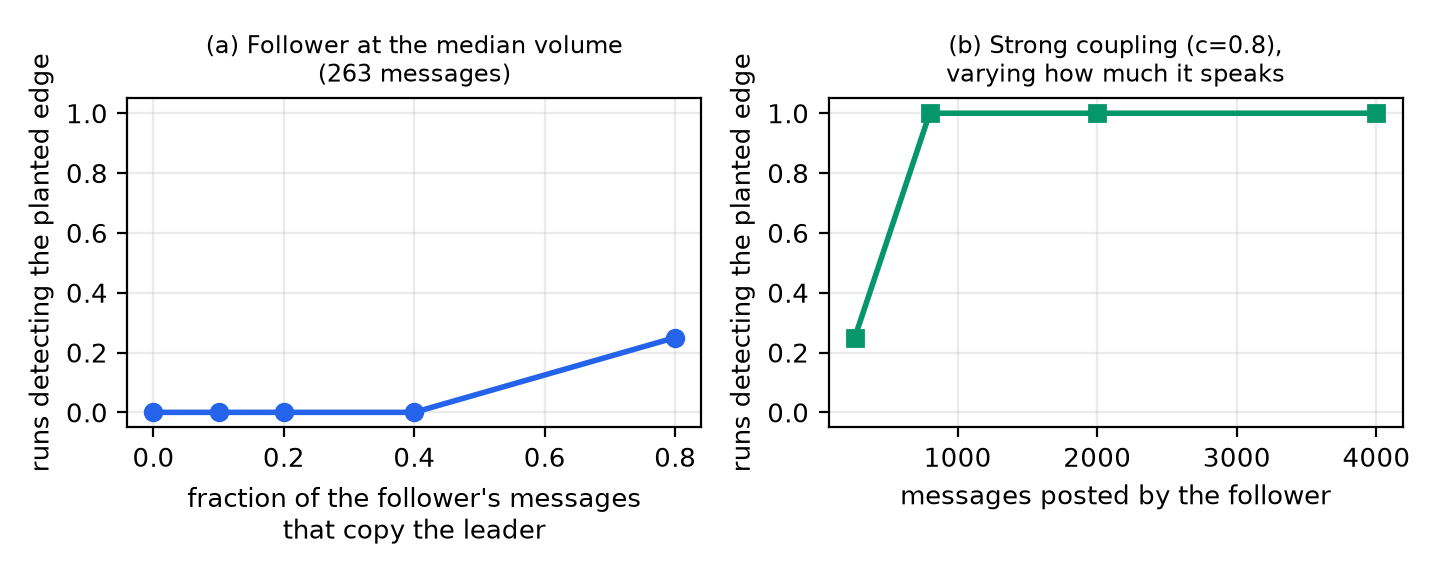
\includegraphics[width=0.92\textwidth]{f4_power.png}
\caption{Detection of a planted follower under the repaired surrogate. Left, varying the fraction of
its messages that copy the leader, at the median agent's volume. Right, varying how much it speaks,
at strong coupling.}
\end{figure}

\paragraph{Humans in the channel.} Main-village \#general is now effectively human-free, with 3 human
messages in the window, so the question has to be asked in open-chat, where 32\% of messages come
from 124 human visitors. Pairwise, with humans collapsed into one node, 19 edges are certified.
Conditioning removes almost all the agent-to-agent structure and little of the rest: \textbf{four
edges survive, of which three run from humans to agents, one is agent to agent, and none run from an
agent to a human.} The asymmetry is not an artifact of the confound. It should be read carefully all
the same: topical dependence from a person to an agent is also what ordinary responsiveness looks
like, so the measurement supports only that the dependence is dyad-specific and directional, not
that anyone is steering a swarm.

\section{Reproducibility, and one limitation of it}

Every number in this paper is recomputed from committed analysis output by a verifier that fails on a
mismatch, and that verifier covers the prose of this paper as well as the figures.

One limitation should be stated plainly. Re-running the counts in the earlier stationarity sweep with
the same seeds and configuration, only one of the eight cells reproduced exactly; the remaining
differences were one or two replicates per cell. Seven of the eight published rates still fell within
the recomputed Wilson intervals, and no conclusion changed. The exception is the zero-drift cell under
the permutation null, where the published 1 of 30 falls just below the recomputed interval of
$[0.035, 0.256]$ for 3 of 30, and no result here depends on that cell.

The generator, estimator and BLAS configuration were investigated and ruled out as the source. The
most likely explanation is a library-level difference, particularly in scikit-learn's $k$-means
implementation within the symboliser, whose output can vary between versions. Every sweep now records
the environment it ran under: Python 3.14.6, numpy 2.5.1, scipy 1.18.0 and scikit-learn 1.9.0,
including the BLAS build and the number of BLAS threads each worker used.

This does not make the previously published counts exactly reproducible. It provides a more clearly
specified environment in which subsequent results can be checked. For that reason I report rates
alongside their confidence intervals rather than exact replicate counts. The distinction between
reproducing a result within its uncertainty and reproducing every individual count matters, and only
the first is claimed.

\section{Conclusion}

Applied to real agent chat, the standard recipe for ``who drives whom'' needs repair before it says
anything. Clock windows cannot separate a message from its answer at the speed agents reply, and what
they certify is matched by a null with no access to meaning. The turn-ordered grid that fixes this
breaks the circular-shift surrogate: family-wise error 0.90 against a nominal 0.05, caused by the
speaker sequence itself. Restricted permutation surrogates repair most of that, but they are flat
under drift rather than calibrated, they are mutually indistinguishable at this precision, and one of
them needs twice the surrogate draws anyone would think to use. A valid surrogate fixes calibration
but not confounding. What survives is small: two dyad-specific edges that do not replicate, an
undetermined answer set by conditioning resolution, and influence running from people into agents and
never back. \textbf{An influence graph should not guide decisions until its error rate, its confound,
its detection floor and its symboliser's fidelity are reported.}

\section*{Limitations}

\begin{itemize}
\item \textbf{Immediate-predecessor only.} The turn-ordered lag-1 measure sees influence from the
message directly before a reply. Influence acting over several turns, or through a room's accumulated
context, is out of scope.
\item \textbf{Discrete approximation to an event process.} Agent chat is event-based in continuous
time. The turn-ordered discretisation with a permutation surrogate is a practical fix, and the
continuous-time comparison above shows what that choice gives up.
\item \textbf{The mechanism behind the real 0.90 is not established.} The generator separates
turn-taking from drift and points at drift, but the largest cell anywhere in the design is 0.365.
\item \textbf{Symbolisation quality cannot be measured on the real logs.} The central result survives
an independent symboliser, but the edge count does not: it moves with alphabet size and with which
messages the topic model is fit on. The floor remains the largest unquantified threat.
\item \textbf{No ground truth in the real logs.} The validity argument rests on planted controls and
on the meaning-free null, not on recovering a known answer.
\item \textbf{Conditioning removes real influence too.} The conditional estimate discards influence
that works by shifting what the channel is talking about, which in a group chat may be a large part
of genuine influence. It is a lower bound on dyadic influence.
\item \textbf{The human result is exploratory.} It rests on one village and one window and should be
read as a lead.
\end{itemize}

\section*{Broader impact and ethics}

This work audits influence detection on a population of AI agents, which is dual-use. Used
defensively it helps an overseer decide what an influence graph is worth, and the main result is
deflationary: it tells practitioners to trust these outputs less, which reduces rather than increases
the chance of acting on a bad attribution. The same tooling could be used to identify the most
influential agent in a swarm in order to target it, or to surveil participants in a channel. Three
properties limit the misuse. The subjects are AI models; the dataset is already public under research
terms and no re-identification is added; and the measure is weak and local, recovering
immediate-predecessor topical dependence rather than any model of how to steer an agent.

The dataset's research terms were followed: research use only, no training on the data, no
re-identification, citation of the source, and notification of the authors of resulting publications.
Human participants appear only as an aggregate node or as anonymised visitor labels, never by name or
handle, and no content attributable to an individual person is reported. Message text and metadata
were read, never model weights or private user data.

The use of a large language model in this work is disclosed in the first-page footnote, as TMLR
requires.

\bibliographystyle{tmlr}
\bibliography{refs}

\end{document}
"               camera-ready
% Use build.py, which runs all of them and checks the anonymous output for leaks.
\providecommand{\TMLRMODE}{submission}
\makeatletter
\def\@tmlrpreprint{preprint}
\def\@tmlraccepted{accepted}
\ifx\TMLRMODE\@tmlrpreprint
  \usepackage[preprint]{tmlr}
\else
  \ifx\TMLRMODE\@tmlraccepted
    \usepackage[accepted]{tmlr}
  \else
    \usepackage{tmlr}
  \fi
\fi
\makeatother

\usepackage{hyperref}
\usepackage{url}
\usepackage{booktabs}
\usepackage{graphicx}
\usepackage{amsmath}

% Gate every identifying string on whether identity may be revealed at all. The flag to test is
% \if@accepted, NOT \if@preprint: tmlr.sty's [preprint] option sets BOTH, so \if@accepted is true
% for the preprint and the camera-ready and false only for the anonymous submission, which is
% exactly the condition wanted. Gating on \if@preprint alone also hid the repository URLs from the
% camera-ready, which is where this paper promises to give them. \if@accepted is internal to
% tmlr.sty, hence the \makeatletter. The anonymous build takes the second argument.
\makeatletter
\newcommand{\ifdeanon}[2]{\if@accepted#1\else#2\fi}
\makeatother
\newcommand{\benchname}{\ifdeanon{SwarmInfluence-Bench}{the benchmark}}

% An unmarked footnote, for the LLM-use disclosure. TMLR's FAQ requires the disclosure and names
% the location: authors must "mention explicitly in their submission that they have used this
% tool", "as a footnote on the first page". Verified against jmlr.org/tmlr/faq.html on 10 Nov 2026.
% It is therefore not optional, and it does not belong in Broader Impact, where it sat until now.
% Nothing in the policy asks for the vendor's name, so none is given.
\newcommand{\disclosurefootnote}[1]{%
  \begingroup\renewcommand\thefootnote{}\footnote{#1}\addtocounter{footnote}{-1}\endgroup}

\title{An Influence Graph Over AI Agents Certifies an Agent That Copies Nobody}

% Hidden by the tmlr package unless [accepted] or [preprint] is given.
\author{\name Manu Nicholas Jacob \email manunicholasjacob@gmail.com \\
        \addr Independent Researcher}

\def\month{11}
\def\year{2026}
\def\openreview{\url{https://openreview.net/forum?id=XXXXXXXXXX}}

\begin{document}
\maketitle

\begin{abstract}
Circular-shift surrogates can produce severely inflated false-positive rates when applied to
turn-ordered multi-agent conversations, reaching a family-wise error rate of 0.90 against a nominal
0.05. A generated benchmark separates two candidate mechanisms and points at non-stationary speaker
activity rather than turn-taking, which suppresses the failure rather than causing it. No setting of
either knob reproduces the observed 0.90, however, so what drives the full real-data failure remains
open. Restricted permutation surrogates substantially reduce the problem. Their error rate is flat
with respect to drift rather than at the nominal level, and for the global within-speaker variant it
depends on how many surrogate draws the null is built from. Calibration alone does not address
confounding, which motivates a conditional estimator validated against a benchmark with planted
ground truth. I also identify a symbolisation-dependent detection limit and develop label-free
diagnostics for it, and show that their calibration does not transport across degradation
mechanisms. The benchmark is released.
\end{abstract}

\disclosurefootnote{\textbf{Use of a large language model.} A large language model was used as an
assistive tool: to help write and run the analysis code, and to help draft this paper. The author is
responsible for every claim, number and figure. All results come from the released code run on the
public dataset, no result or reference is fabricated, and every number in this paper is recomputed
from committed analysis output by a verifier that fails the build on a mismatch.}

\section{Introduction}

When AI agents interact in a shared channel, it is useful to understand how they influence one
another. Information-theoretic methods offer a way to measure this through lagged transfer entropy,
surrogate testing, and per-agent influence scores. They are attractive because they require no
labels and no access to model internals, only a record of who said what and when. The reliability of
those measurements is what this paper examines.

Almost every demonstration of these detectors runs on synthetic traces with a planted leader, where
the analyst controls timing and vocabulary. Real agent chat is asynchronous, bursty, and written in
open language. The narrower question here is whether the standard recipe, applied to real agent
logs, returns anything an overseer should act on.

The audit runs on the AI Village corpus \citep{aidigest2026}, in which frontier models share chat
channels over eighteen months across four villages differing in size, lifetime and tempo, applying
the checks a reader should demand: planted controls, a meaning-free symboliser, replication in a
held-out window, and sensitivity to every parameter that had to be chosen.

\begin{enumerate}
\item The conventional circular-shift surrogate is \textbf{invalid} on turn-ordered agent chat: a
family-wise error rate of 0.90 against a nominal 0.05, caused by the structure of the speaker
sequence itself.
\item Restricted permutation surrogates restore most of the calibration, and re-certifying under one
\textbf{scrambles rather than shrinks} the answer: one channel loses all 11 of its edges, another
gains 15.
\item The three restricted variants are \textbf{mutually indistinguishable} at the precision reached
here, so the choice between them cannot be justified on error rate. The global within-speaker
variant additionally needs on the order of 200 surrogate draws, and over-fires by roughly a factor
of two at 100.
\item Calibration is not confounding, so a conditional estimate is added and validated on a released
benchmark with a known influence graph: common-cause false edges fall from 22.3 to 0.33, and on the
planted-edge instances precision rises from 0.17 to 0.80 with no loss of recall or power.
\item The same benchmark exposes a \textbf{symbolisation floor}. Below roughly 0.44 adjusted Rand
index between symboliser and truth, detection collapses whatever the estimator. Label-free
diagnostics detect that floor, but their calibration does not transport across degradation
mechanisms, and I report where it fails.
\item On the real channels two edges stand at every conditioning resolution, 18 are
\textbf{undetermined} between 0 and 13, none replicates out of sample, and what survives alongside
humans runs from people to agents.
\end{enumerate}

\section{Related work}

\paragraph{Transfer entropy and surrogates.} Transfer entropy \citep{schreiber2000} measures how much
a source's past reduces uncertainty about a target's next symbol beyond the target's own past.
Plug-in estimators are biased upward on short series, so significance rests on surrogate data, with
family-wise error controlled by a max-T test \citep{westfall1993}. The usual surrogate is a circular
time shift of the source.

\paragraph{Event-based data breaks the shift surrogate.} \citet{shorten2021}, on neural spike trains,
show that the conventional source-time-shift surrogate fails to represent the null hypothesis of
conditional independence for event-based processes, and adapt to that setting the nearest-neighbour
local permutation scheme of \citet{runge2018}. Agent chat is event-based in that sense: messages are
events in continuous time, not samples of a clocked signal. The correction is not a contribution of
this paper. The contribution is showing that the same failure carries over to multi-agent safety
monitoring, and that it can be severe enough to create apparent leaders where none exist.

\paragraph{The same failure, concurrently, in multi-agent reinforcement learning.}
\citet{papadopoulos2026} report a closely related surrogate failure in multi-agent
reinforcement-learning action series. Their agent pairs have zero influence by construction, yet
circular time shifts produce false-positive rates of 100\% and 98.2\% against a nominal 0.05. A
plain permutation surrogate fares no better in their setting, at 100.00\% and 99.95\%. Their
proposed correction restricts permutations to blocks of training time, which returns the rates to
5.25\% and 5.50\%.

There are important differences between their setting and this one. Their data consist of binary
actions recorded over twelve thousand training rounds, whereas these data are symbolised
natural-language messages arranged on a turn-ordered conversational grid. Their non-stationarity
comes from monotone drift associated with annealing exploration; here the relevant non-stationarity
appears in the speaker sequence. Neither result should be taken as a direct extension of the other.

Nevertheless, the fact that both approaches rely on restricted permutations is worth noting. Their
permutation blocks are defined by training time, while mine are defined by an agent's own speaking
positions. This provides convergent evidence that unrestricted temporal rearrangement can be
problematic in non-stationary multi-agent data. Their findings also serve as a useful warning for
the approach taken here, and the warning has a measured form rather than a rhetorical one: in their
data the unrestricted permutation failed as completely as the time shift, at 100.00\% against a
nominal 0.05. Permutation-based surrogates are not automatically protected against
non-stationarity, and what protects the one used here is the restriction, not the permutation. I
claim no priority over their result and view the two studies as complementary, addressing different
forms of structured multi-agent data.

\paragraph{Oversight under a budget.} AI-control research frames monitoring as resource constrained,
with a cost for false positives \citep{greenblatt2024}. An influence graph is one such measurement,
and its error rate is the concern here.

\paragraph{Clustering stability.} The idea of using clustering stability as a label-free quality
indicator is not new. It has a substantial history, including \citet{benhur2002},
\citet{lange2004}, von Luxburg's review of clustering stability \citep{vonluxburg2010}, and
\citet{tibshirani2005} on prediction strength. What is different in Section~\ref{sec:floor} is the
calibration of these diagnostics against a detection-performance floor rather than against cluster
recovery alone.

\section{Data and representation}

The AI Village dataset ships one gzipped-JSONL table per village. Four villages are used, differing
enough to test whether any finding is a property of one channel.

\begin{table}[h]
\centering
\begin{tabular}{lrrrrl}
\toprule
village & agent messages & agents & lifetime & human messages & busiest room \\
\midrule
main      & 205,726 & 58  & 576 days & 10,029 & \#general (166,715, 81\%) \\
open-chat &  35,483 & 23  &  66 days & 12,264 & \#general (all) \\
swarm     &   3,848 & 133 &   1 day  &      5 & room a (3,846) \\
game-jam  &     838 & 6   &   3 days &     36 & per-team rooms \\
\bottomrule
\end{tabular}
\caption{The four villages. A 2026 scaffolding change scopes each agent to its current room's
context, so the busiest room of each village is a self-contained influence substrate and is analysed
alone.}
\end{table}

The primary window is the final fourteen days of main-village \#general, 17 to 31 October 2026,
holding 8,800 agent messages. Twenty-two models posted at least 50 messages each and the directed
test uses the 15 busiest, giving 7,958 message events. Two scaffolding facts are disclosed rather
than corrected: the automated nudger was off throughout, and the unused \#best and \#rest rooms were
soft-deleted mid-window, which does not touch \#general.

\subsection{From open language to symbols}

Transfer entropy needs discrete symbols, so each message is mapped to a small alphabet before
influence is estimated, and that mapping is kept separate from the estimator. A topic symboliser
(TF-IDF then $k$-means, $k=8$) gives a message its topic cluster id, so paraphrases of one idea share
a symbol. A hash symboliser, a stable hash of the normalised text into $k=8$ buckets, has no notion
of meaning and serves as a null: an edge appearing under both lives in timing alone.

\subsection{The lag problem, and why clock windows cannot solve it}

A lag-1 transfer entropy compares window $t-1$ with window $t$, so influence landing inside one
window is invisible to it. Agent chat makes this binding. Among the fifteen analysed agents the gap
between consecutive messages by different speakers has a median of 28.1 seconds (25th percentile
9.2, 75th 66.2, 95th 159.3), so turn-taking is a seconds-scale process while any clock window wide
enough to hold two speakers is minutes wide and swallows both a message and its answer.

Both horns are measurable. At 30 seconds only 1.2\% of agent-windows hold a message, while 32.0\% of
replies already land in the same window as what they answer, rising to 84.4\% at five minutes. At
every width tried, the meaning-free hash null certifies comparably many edges, and more at five
minutes: 9 against 12 at thirty seconds, 17 against 19 at one minute, 27 against 44 at fifteen, and
19 against 17 at five. Whatever clock-window transfer entropy was detecting there, it was not shared
meaning.

\begin{figure}[h]
\centering
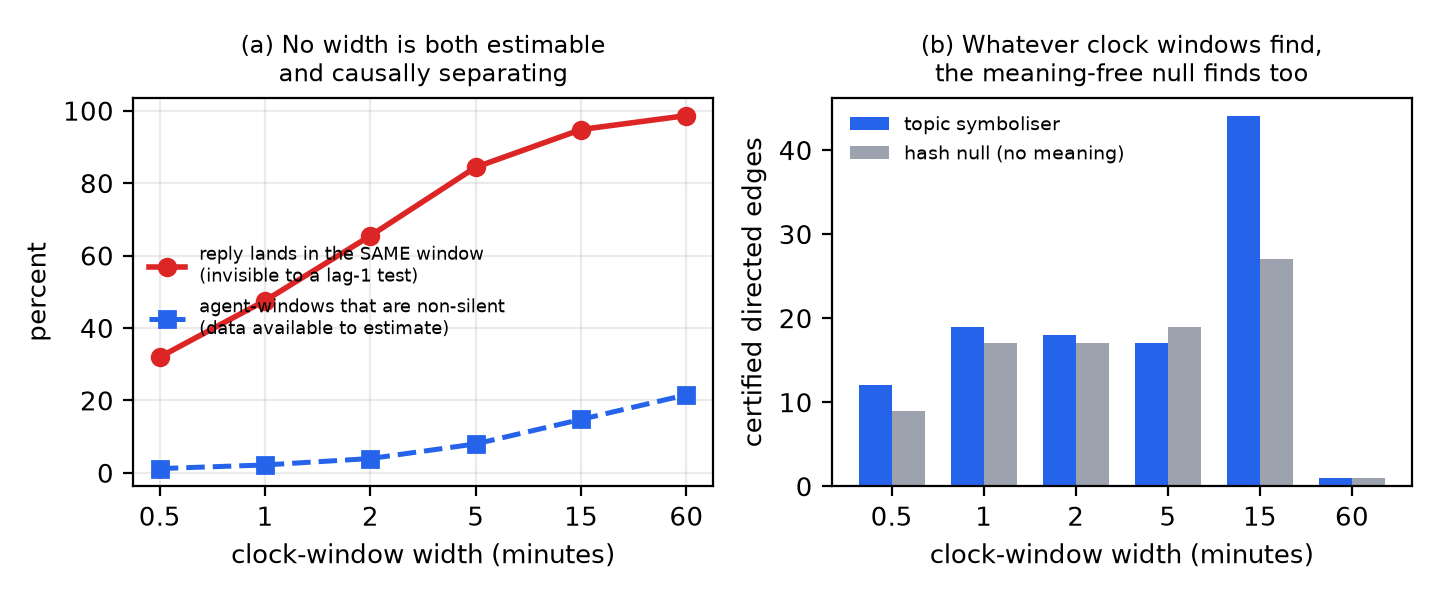
\includegraphics[width=0.92\textwidth]{f1_clock.png}
\caption{Clock-window transfer entropy on the 15 analysed agents of main-village \#general. Left,
the two failure modes as a function of window width. Right, edges certified under the topic
symboliser against the meaning-free hash null.}
\end{figure}

The bind is avoided by ordering messages canonically and letting one message be one tick. Each
agent's series carries its symbol where it spoke and a silent symbol elsewhere, so the lag-1
comparison is between a message and the one immediately before it. The cost is that the measure
captures immediate-predecessor influence only.

\section{The surrogate failure, and two explanations that did not hold}
\label{sec:failure}

An agent is planted into the real stream, drawing its symbols from the channel's marginal and
coupled to nothing at all. It is certified as driving something in 3 of 8 runs when it posts 50
messages, and in 8 of 8 at 100, 263, 600 and 1500 messages, with the mean largest $z$ rising from 5.6
to 12.3, 21.7, 38.3 and 71.7. The error grows with how much the agent speaks, which rules out a
small-sample explanation.

A planted agent could be dismissed as artificial, so the error rate is also measured directly.
Keeping the real speaker sequence and permuting the symbols globally leaves data with no directed
topical influence by construction. The shift surrogate certifies at least one edge in 9 of 10 such
replicates, a family-wise error rate of 0.90 against a nominal 0.05.

\paragraph{What breaks it is the speaker sequence.} Destroying one structure at a time isolates the
cause. Keeping the real speaker order and shuffling only symbols, the shift surrogate fires in 10 of
10 replicates; randomising the speaker order as well drops it to 0 of 10; uniform symbols with the
real order still give 6 of 10. So the driver is the structure of the speaker sequence, not the
symbol distribution and not sparsity. That sequence is far from random in two ways at once: it
repeats a speaker 36\% of the time and returns after one message 38\% of the time, and each agent's
activity is strongly non-stationary, with a median block-share coefficient of variation of 0.79.
Shuffling the order destroys both at once, so this ablation cannot say which of the two mattered.

\subsection{Two explanations I proposed, and the benchmark refuted both}

I initially attributed the failure to mutual exclusivity: only one agent can speak at each tick, so
shifting individual timelines could create overlaps that never occurred in the original
conversation. The benchmark did not support this explanation. A generated channel with exactly one
speaker per tick and steady activity produced an error rate of just 0.025, 95\% Wilson
$[0.011, 0.057]$, far below the 0.90 observed in the real data. Mutual exclusivity alone therefore
cannot explain the failure.

I then suspected turn-taking. In the real channel, speakers repeat 36\% of the time and return after
exactly one message 38\% of the time. However, adding a Markov speaker chain to the generator
produced the opposite result. Turn-taking suppressed the error rather than increasing it. At the
nominal knob values and with no drift the surrogate certified nothing at all across 200 replicates,
while removing turn-taking and introducing drift raised the rate to 0.365. The contribution from
drift was $+0.340$, compared with $-0.025$ for turn-taking. The same inversion appears in the arm
calibrated so that the generated channel reproduces the real channel's measured repeat, return and
block-share statistics rather than merely carrying those numbers as settings: there, turn-taking
alone also certifies nothing, and drift alone gives 0.065.

Neither mechanism, nor their combination in the tested design, reproduced the real-data error rate of
0.90. The largest cell anywhere in the design is 0.365. The real-data ablation removes turn-taking
and non-stationarity together, while the generator separates them. The results point to
non-stationary activity, but the remaining gap means the mechanism behind the full real-data failure
is not yet established.

Every figure above comes from the run at 200 surrogate draws. The first version of this analysis
used 100, which inflates both nulls on the same 2,400 instances: the circular shift fires 53 times
where the 200-draw run does not, against 18 the other way (exact McNemar $p = 3.9 \times 10^{-5}$),
and the permutation surrogate 83 against 20 ($p = 2.7 \times 10^{-10}$). Every qualitative conclusion
in this section is the same at both settings, which is why they are worth stating at all. The
numbers are not, so the draw count belongs in the caption.

\section{The repair, compared}
\label{sec:repair}

Following the local-permutation idea of \citet{runge2018} as adapted by \citet{shorten2021}, each
source keeps its speaking positions and only its symbols are permuted among them. Speaking pattern,
sparsity and turn-taking are preserved exactly, and only the correspondence between symbol and time
is destroyed. On the same destroyed-structure real data the family-wise error rate falls to 0.063
over 300 replicates, 95\% Wilson $[0.041, 0.097]$. The planted uncoupled agent is never certified: 0
of 5 at both 263 and 1500 messages, with mean max $z$ of 2.8 in each case against 22.0 and 68.3
under the shift surrogate.

\begin{figure}[h]
\centering
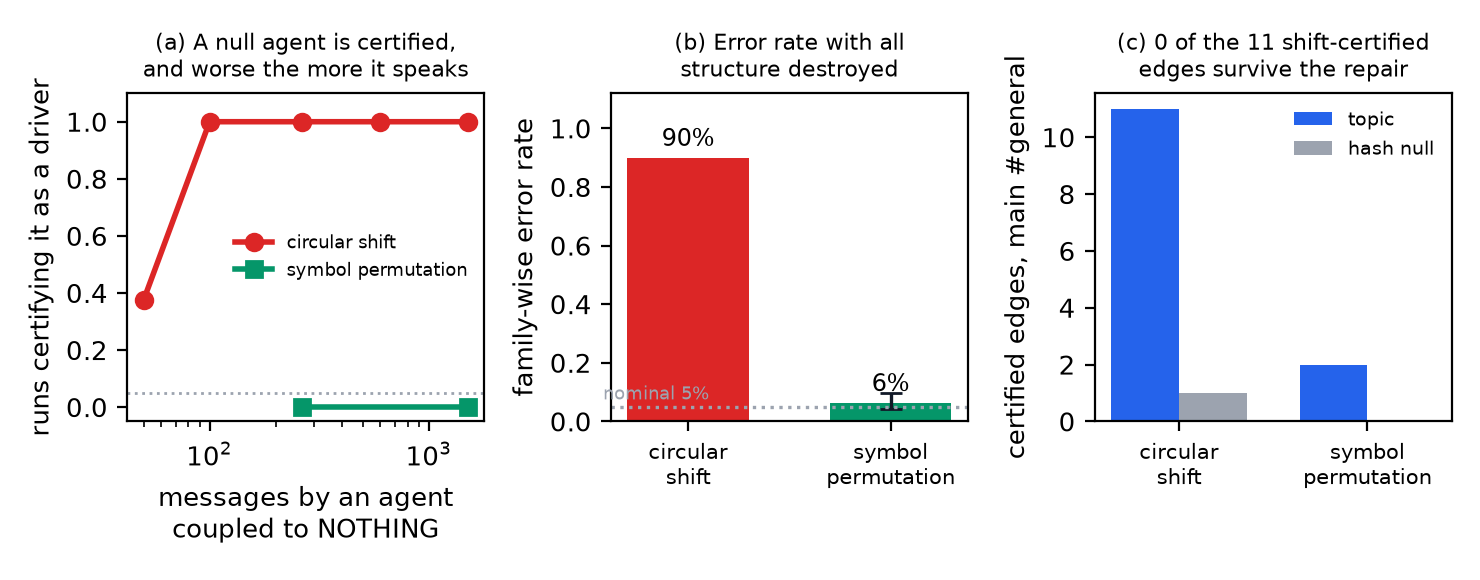
\includegraphics[width=\textwidth]{f2_null.png}
\caption{Left, how often an agent coupled to nothing is certified as a driver, under each surrogate.
Middle, family-wise error rate measured on data with all structure destroyed, with a Wilson
interval; the dotted line is the nominal 0.05. Right, what each surrogate certifies on the real
channel.}
\end{figure}

\subsection{How many surrogate draws are needed}

The number of surrogate draws matters more than I initially appreciated. In a paired comparison of
300 instances, where all four surrogates run on identical symbol grids so the outcomes are paired,
the global permutation surrogate produced a false-positive rate of 0.1167 with 100 draws, falling to
0.0700 with 200 draws, 95\% Wilson $[0.046, 0.105]$. This difference is statistically significant
(exact McNemar $p = 0.0043$). The block-local and Runge local permutations were less sensitive to the
increase: their corresponding rates changed from 0.0900 to 0.0767 and from 0.0967 to 0.0800.

At 200 draws, the global permutation's interval covers the nominal 0.05 and overlaps the real-data
estimate of 0.0633 $[0.0409, 0.0968]$. The real-data result is therefore corroborated rather than
overstated. For practical use, the important point is that reducing the number of surrogate draws
can materially change the result. In particular, the global permutation over-fires at 100 draws by
approximately a factor of two. I would therefore not treat the choice of draw count as a minor
computational detail.

The same correction applies to the benchmark-wide estimate. That figure was 0.0942 at 100 draws.
Repeating all 2,400 instances at 200 draws gives \textbf{0.0679}, 95\% Wilson $[0.0585, 0.0787]$,
and the paired difference is large: 83 instances fire at 100 draws and not at 200, against 20 the
other way, $p = 2.7 \times 10^{-10}$. The conclusion it supports is unchanged, because the interval
still excludes the nominal 0.05. So the permutation repair does carry a residual inflation on clean
generated data, but it is about a third above nominal rather than nearly double.

One limit on this recommendation. I compared 100 draws against 200 and did not test any larger
value, so what the experiment establishes is that 100 is too few, not that 200 is enough. Two
hundred is a lower bound on the draw count rather than a converged setting, and a practitioner whose
conclusions sit near a decision boundary should check their own sensitivity rather than adopt the
number.

\subsection{Choosing a repair, when the error rate cannot choose}

The comparison of the three permutation-based repairs does not produce a clear winner. All four
surrogates were evaluated on identical symbol grids across 300 pure-null replicates, so the
comparison reflects differences between the null models rather than differences between datasets.

\begin{table}[h]
\centering
\begin{tabular}{lrrrl}
\toprule
surrogate & FWER, 100 draws & FWER, 200 draws & 95\% Wilson at 200 & nominal 0.05 \\
\midrule
circular shift                   & 0.0433 & \textbf{0.0333} & $[0.018, 0.060]$ & inside \\
global within-speaker permutation & 0.1167 & \textbf{0.0700} & $[0.046, 0.105]$ & inside \\
block-local permutation          & 0.0900 & \textbf{0.0767} & $[0.052, 0.112]$ & excluded \\
local permutation \citep{runge2018} & 0.0967 & \textbf{0.0800} & $[0.054, 0.116]$ & excluded \\
\bottomrule
\end{tabular}
\caption{Four surrogates on identical symbol grids, 300 pure-null replicates, at both draw counts.}
\end{table}

At 200 draws, paired on the same 300 instances, the circular shift is not significantly different
from the global permutation ($p = 0.0614$), although it differs from block-local permutation
($p = 0.0294$) and from Runge's local permutation ($p = 0.0201$). At 100 draws it differed from all
three, which is the draw-count artifact again. The three repairs remain statistically
indistinguishable from one another, with pairwise $p$-values of 0.85, 0.65 and 1.00. The apparent
differences in their error rates are not sufficient to establish a ranking.

Choosing between them therefore requires more than calibration, and two readings pull against each
other. Runge's local permutation has the strongest methodological justification for preserving the
structure it is intended to preserve, and it follows the approach adapted to event data by
\citet{shorten2021}. Block-local permutation is more heuristic and introduces a free parameter that
has not been tuned. Global permutation is the simplest. On the other hand, the global permutation has
the most favourable interval relative to the nominal rate, and is the only repair that costs nothing
measurable against the shift on clean stationary data, although neither difference is statistically
established. I do not consider the observed error rates sufficient to select one repair over the
others. The choice should be guided by the structure the null is intended to preserve and the
assumptions that can be justified for the data.

\subsection{When to use the repair}

A drift sweep gives the practical reading. Across 150 replicates per cell at 200 surrogate draws,
the circular shift degrades steadily as activity drift increases while the three repairs do not.

\begin{table}[h]
\centering
\begin{tabular}{lrrrr}
\toprule
activity drift & circular shift & global permutation & block-local & local \\
\midrule
0.0 & \textbf{0.013} & 0.093 & 0.080 & 0.093 \\
0.3 & 0.100 & 0.100 & 0.093 & 0.120 \\
0.6 & \textbf{0.193} & 0.053 & 0.047 & 0.067 \\
0.9 & \textbf{0.380} & 0.087 & 0.080 & 0.080 \\
\bottomrule
\end{tabular}
\caption{Family-wise error on pure nulls as activity drift increases, 150 replicates per cell, 200
surrogate draws. Every certified edge is a false positive by construction.}
\end{table}

The pattern is supported by a formal trend test rather than by eye. A Cochran-Armitage test across
the four ordered drift levels gives the circular shift $z = 8.667$, $p < 10^{-15}$, and gives every
repair nothing: $p = 0.51$ for the global permutation, 0.63 for block-local and 0.37 for local. The
same pattern holds at both surrogate draw counts, so it does not depend on that choice.

The repairs are therefore flat under drift rather than calibrated. Only one of the four global
permutation intervals covers the nominal 0.05, and the rest sit nearer 0.09, so what the repair buys
is insensitivity to drift rather than correctness. One asymmetry should be stated rather than
hidden: block-local covers nominal in three of the four cells where the global repair covers one.
The two remain pairwise indistinguishable, so this is not grounds to switch the recommendation, but
it does mean the global repair cannot be described as the best-calibrated under drift.

The results also show why the repair should not be treated as universally preferable. At zero drift
the circular shift has an error rate of 0.013, while the three repairs are all around 0.08 to 0.09.
That advantage is gone by the first drift step: at drift 0.3 the shift reads 0.100 against the global
permutation's 0.100 and block-local's 0.093, so the crossover falls between drift 0.0 and 0.3 rather
than at some higher level. By drift 0.6 the shift is roughly four times the repairs. If a channel has
been checked and found stationary, the circular shift may be sufficient. When activity is
non-stationary the repairs are the more stable choice, and the margin for error on that judgement is
narrow, because the crossover arrives by the first drift level tested.

\section{Continuous time, and what the repair cannot test}

An earlier analysis identified continuous-time estimation as the principled option for event data
but did not evaluate it. Running the continuous-time estimator CoTETE on both channels certifies 0
edges in either case, compared with 2 for main-village and 18 for open-chat under the discrete,
turn-ordered analysis. Its highest $z$-scores are 3.062 and 3.980, below the respective max-T
thresholds of 4.171 and 4.308.

At first these results might appear to contradict the symbol-based analysis. The two estimators
operate on different information, however. CoTETE's public API takes event times with no symbol
channel, while the transfer-entropy analysis here uses topic symbols. To test whether this
difference explains the results, I reduced the data to timing alone, replacing every spoken symbol
with the same code. Under this representation the estimator used here also detects 0 edges in both
channels, matching CoTETE. Using the circular-shift surrogate instead produces 12 and 3 edges. So
neither method detects relationships from event timing alone in these channels, and the edges found
by the symbol-based analysis depend on symbol correspondence, which the continuous-time estimator
cannot access.

Two caveats attach to those $z$-scores, and the second attaches to the larger of them. Point
estimates from this estimator are stochastic to about 17\% across repeated runs, so none of these
values should be read to more than two significant figures. And open-chat's highest $z$, the 3.980,
belongs to the one pair whose surrogate draws mostly failed: it needed 1,936 failed draws to obtain
100 successes, a 4.9\% success rate. Those surrogates are conditioned on being estimable, so that
pair's null is biased in an unknown direction. The conclusion does not rest on it, since that pair
falls below threshold and so does every other pair, but the number should not be quoted as a clean
measurement. The failures themselves were a defect rather than a property of the data: an enlarged
exclusion window can empty the neighbour search on sparse bursty event trains and raise an error
that terminates a whole pair, with no handling at the public entry point. This has been reported
upstream.

There is also a fundamental limitation in applying the recommended permutation surrogate to
timing-only data. When every event carries the same symbol, permuting those symbols changes nothing.
The observed statistic and the surrogate null are identical, making the test exactly degenerate:
standard deviation 0 across all 210 pairs and $p = 1.0$ everywhere. \textbf{The repair has zero power
against timing structure by construction.} The permutation surrogate is appropriate for testing
relationships in the symbol sequence, but it does not answer whether relationships exist in event
timing. These are different questions, and choosing one null means giving up the ability to test the
other with that procedure.

\section{Confounding, and what conditioning removes}

A valid surrogate fixes calibration but not confounding. If every agent tracks a drifting channel
topic, every pair is genuinely dependent through the channel, and pairwise transfer entropy cannot
tell that from direct influence. I therefore also report a \textbf{conditional} estimate, which asks
whether a source's last message adds anything about a target's next one beyond the target's own
history and the channel's recent state. The conditioning variable is the modal symbol of the last
twelve messages, excluding the immediately preceding one so that it does not simply restate the
source.

On a generated benchmark whose decisive instances contain no influence while every agent tracks a
shared drifting topic, so that any certified edge is common cause, pairwise transfer entropy
certifies \textbf{22.3} edges on average and conditioning takes that to \textbf{0.33}, lifting pooled
precision on the four-edge instances from 0.17 to \textbf{0.80} at a recall of 1.0 either way. Across
couplings from 0.05 to 0.8 the conditional test still finds the planted edge in 3 of 3 runs, so the
gain costs no power.

The benchmark flatters the conditional estimator, since its common cause is a shared modal topic and
the conditioning variable is the channel's modal topic. The real channels are harder, and
conditioning there costs degrees of freedom: a 9-symbol alphabet with a 9-valued context gives 6,561
cells against about 7,900 ticks, so that variable is also coarsened to 4 and 2 values.

\begin{table}[h]
\centering
\begin{tabular}{lrrrr}
\toprule
channel & pairwise & conditional, 9 values & 4 values & 2 values \\
\midrule
main \#general      & 2  & \textbf{2, the same two edges} & 2 & 3 \\
open-chat \#general & 18 & \textbf{0} & \textbf{7} & \textbf{13} \\
swarm, room a       & 1  & \textbf{0} & & \\
\bottomrule
\end{tabular}
\caption{Conditioning at three resolutions. Main-village's two edges are robust to that choice;
open-chat's zero is not.}
\end{table}

At the finest resolution the open-chat test is degenerate, its surrogate sitting above the observed
statistic for 65\% of pairs with the largest $z$ in the family only 4.4, so it is failing to reject
rather than finding nothing to reject. Open-chat's structure therefore remains
\textbf{undetermined}: depending on the conditioning resolution, between 0 and 13 of its 18 edges may
survive. That resolution is a free parameter an analyst would set once and never revisit. This is a
property of the channel rather than the estimator: on structure-free real data the conditional test
fires in 2 of 40 replicates, an error rate of 0.05 with a mean $z$ of $-0.001$, so it is nominal
rather than conservative.

\section{The symbolisation floor}
\label{sec:floor}

Everything these methods produce is downstream of turning text into symbols. On the benchmark, where
the underlying topics are known, detection performance drops sharply when agreement between the
symboliser and the ground truth falls below roughly ARI 0.44, and this behaviour appears across the
tested estimators. Importantly, the false-positive rate can look \emph{better} below this point,
because the shared topic structure needed to produce confounded detections is no longer represented
reliably. A pipeline that stops detecting relationships may therefore have lost the signal it needs
rather than become more reliable, and nothing downstream of the symboliser can tell those apart.

\subsection{Detecting the floor without labels}

That degradation can be detected without ground-truth labels. Across the nine-level benchmark sweep,
three statistics separate the below-floor cases with zero errors: seed stability at a threshold of
0.623, agreement with LSA at 0.646, and the Calinski-Harabasz index at 138.9. Seed stability here is
the \textbf{minimum} pairwise agreement across seeds, not the mean; the mean variant makes one error,
at a different threshold of 0.791. Silhouette has the strongest correlation with true ARI, at 0.979,
but is not useful for identifying the boundary because its threshold falls within a gap of just
0.002. A statistic that tracks clustering quality most closely is not necessarily the best one for
making a classification decision.

Error count cannot choose among the three that were perfect, so I tested whether each threshold still
means what it meant when the channel changes for reasons other than topic separability. Applying each
cut unchanged to thirty cells that vary turn-taking, drift, agent count, volume skew, message length
and corpus size, twenty-seven of which hold true ARI at exactly 1.000:

\begin{table}[h]
\centering
\begin{tabular}{lrrrr}
\toprule
diagnostic & cut & errors where fitted & errors, nuisance set & of those at true ARI 1.000 \\
\midrule
seed stability, min across seeds & 0.623 & 0 & 2 & \textbf{0} \\
LSA agreement                    & 0.646 & 0 & 2 & \textbf{0} \\
Calinski-Harabasz                & 138.9 & 0 & 6 & \textbf{3} \\
\bottomrule
\end{tabular}
\caption{Whether a cut fitted on the vocabulary-overlap mechanism survives a change in the channel
that is not a change in topic separability.}
\end{table}

The two bounded statistics err only on the short-message cells, where the symbolisation genuinely has
degraded. Calinski-Harabasz additionally condemns all three cells whose true ARI is exactly 1.000,
for no reason beyond the corpus holding 2,000 messages rather than 8,000, where it reads 76 to 77
against its own cut of 138.9. It is unbounded and grows with sample size, so a published numeric
threshold for it carries no meaning on another corpus. That is why I recommend the two bounded
statistics and not the index that matched them on error count. \textbf{A cut that moves with the
corpus is not a floor cut.}

This is not a weak statistic being discarded on a technicality. Calinski-Harabasz correlates with
true ARI at 0.973, almost as closely as silhouette, and unlike silhouette it classifies the floor
perfectly where it was fitted. It still cannot carry a published threshold. That is the sharper form
of the point above: neither the statistic that tracks quality most closely nor the one that
classifies best on the fitting mechanism is necessarily the one whose cut another researcher can
reuse.

There are important limits to this result. The effective sample size is nine rather than 54, because
the classification label is determined by overlap level. There are no observations between ARI 0.444
and 0.222, so the exact location of the boundary within that interval remains unknown. These
diagnostics classify whether a result is below the tested detection floor; they do not estimate ARI,
and their behaviour is flat between 0.68 and 1.00, and not even monotone there. The benchmark also
uses a single degradation mechanism with a known and correct value of $k$, whereas the true number of
topics in real conversations is unknown. I therefore treat 0.44 as a benchmark-specific, bracketed
result rather than a universal threshold.

\subsection{A contradiction the diagnostic lost}

I initially used these diagnostics to classify one real channel, open-chat, as below the
symbolisation floor. That conclusion did not agree with the channel's measured results: open-chat
certified 18 and 22 edges under the two symbolisers, compared with 2 and 1 for main-village, and its
hash-based null certified zero edges. Rather than treating this disagreement as evidence that the
original measurements were wrong, I revisited the diagnostic itself.

The problem was the choice of $k$. Repeating the comparison with the same channels, loader and window
reproduced the published $k=8$ results to the digit. At $k=4$, however, open-chat reached stability
scores of 0.950 and 0.978, the highest values produced by either channel across the tested settings,
and both exceeded the diagnostic thresholds. The earlier below-floor classification was therefore a
conclusion about one arbitrary choice of $k$, not a reliable statement about the channel. Message
length does not explain the difference either: 27.1\% of main-village messages contain fewer than
five tokens, compared with 2.3\% in open-chat, so the short-message channel is the one the diagnostic
cleared.

This correction changes how the symbolisation results should be read, and it withdrew three claims.

\begin{enumerate}
\item \textbf{The claim that no topic signal remains below the floor is too strong.} The
circular-shift surrogate recovers all four planted edges at every tested overlap level, including
0.95, where ARI is 0.011. The observed collapse is in the permutation null, not necessarily in the
underlying data.
\item \textbf{ARI 0.44 cannot be treated as a universal detection threshold.} When the shared-topic
parameter is 0, detection continues down to ARI 0.296, so the boundary depends on both the
symboliser and the channel.
\item \textbf{Edge counts cannot be used as a measure of symboliser quality.} Even at ARI exactly
1.000, changing the shared-topic parameter alone moves the permutation edge count from 5 to 78.
\end{enumerate}

The diagnostics also do not transfer reliably outside the mechanism on which they were evaluated.
Their balanced accuracy falls from 1.00 to 0.75 and 0.571 under a known mismatch in $k$. All seven
errors made by seed stability are false below-floor classifications, and in every one of those cases
the detector still identifies all planted edges; of the fourteen cells it condemned, eleven had full
conditional recall. The failure direction is the dangerous one: it condemns working symbolisations.

This was an important correction to my own interpretation. I introduced a diagnostic to check whether
the symbolisation was reliable, applied it to the real channels, and found that it contradicted
measurements already in hand. Investigating that contradiction showed the diagnostic was sensitive to
an arbitrary modelling choice. The result is not that the original measurements were wrong, but that
the control was being asked to support a broader conclusion than the evidence allowed. These
diagnostics remain useful within their tested setting, and \textbf{no channel-level floor verdict
should be issued from a single $k$}.

\section{The benchmark}

Real logs have no ground truth, so the common-cause question could not be settled on them. The
generator used here makes the influence graph known by construction: it decides, in code, who speaks
at which tick, on which topic, and who reacts to whom. Surface text is a separate, replaceable layer
drawn from disjoint per-topic vocabularies, so the whole thing runs offline and a detector still has
to symbolise raw text rather than read the labels. Turn-taking and activity drift are independent
knobs, so the two can be varied one at a time, and the generator reproduces its earlier behaviour
bit for bit when both are zero.

\benchname{} is released with 150 tests covering the generator, the detector harness, the text layer,
the floor analysis and the turn-taking factorial.
\ifdeanon{Code and benchmark:
\url{https://github.com/manunicholasjacob/swarm-influence-bench} and
\url{https://github.com/manunicholasjacob/swarm-influence-audit}.}{Code and benchmark are publicly
released; the links are withheld here for anonymity and will be given in the camera-ready version.}

One property of the benchmark must be stated when its numbers are quoted. Planting an edge displaces
other agents' speaking turns, so the generated instances contain real lag-1 dependencies that the
label set does not list. Precision measured against those labels is therefore a \textbf{lower bound}
for any detector, and what the benchmark supports is the comparison between two estimators rather
than the absolute value of either.

\section{What an overseer should do}

Six inexpensive controls should be included whenever an influence graph over an agent channel is
published.

\begin{enumerate}
\item \textbf{Plant an agent coupled to nothing, at your channel's volumes, and check it is not
certified.} This one test would have caught the failure reported here, at one run per volume.
\item \textbf{Measure the error rate directly}, by destroying the structure your method claims to
find and checking the family-wise rate is near nominal. If it is not, your surrogate does not match
your data.
\item \textbf{Preserve the speaker sequence in your surrogate.} Any surrogate that moves an agent's
messages in time will disturb it, and \citet{shorten2021} is the principled route. Use at least 200
surrogate draws, because at 100 the global within-speaker permutation over-fires by roughly a factor
of two.
\item \textbf{Establish the detection floor before interpreting an absence.} ``No edges'' and ``no
influence'' are different claims.
\item \textbf{Condition on the channel, report both numbers, and sweep the resolution.} Pairwise and
conditional bound the answer, and the gap between them is the result. Conditioning costs cells, so
check whether your answer is an artifact of how finely you conditioned. On one channel here it was.
\item \textbf{Report how well your symboliser agrees with the truth, on data where you know it.}
Everything is downstream of turning text into symbols, and below roughly ARI 0.44 detection
collapses whatever the estimator. I have found this control in no influence-detection paper, and it
is also the one that cannot be run on real logs, which is why the floor remains the largest
unquantified threat here.
\end{enumerate}

Two habits follow: publish a meaning-free null's count beside the real one, and require held-out
replication before calling a graph a structure.

\section{The real channels, and what survives}

Re-running every channel under the repaired surrogate changes the answers, and not in one direction.

\begin{table}[h]
\centering
\begin{tabular}{lrrr}
\toprule
channel & window messages & shift: topic / hash & permutation: topic / hash \\
\midrule
main \#general      & 8,800 & 11 / 1 & 2 / 0 \\
open-chat \#general & 8,226 & 3 / 0  & 18 / 0 \\
swarm, room a       & 3,846 & 2 / 1  & 1 / 0 \\
\bottomrule
\end{tabular}
\caption{The same channels under both surrogates, with the meaning-free hash null beside each.}
\end{table}

In main-village, \textbf{none} of the 11 edges the standard recipe certifies survives the repair, and
the two the valid surrogate certifies were not among them. In open-chat the correction runs the other
way, 3 edges becoming 18, because pathological pairs inflate the max-T threshold and raise the bar
for everything else. An invalid surrogate does not simply add false positives; it scrambles the
result.

Main-village's two edges are the strongest thing here and they are still not a finding, because they
do not replicate: the adjacent fourteen-day window certifies nothing at all under either estimator.
Given the detection floor, that silence is as consistent with the test sitting near its limit as with
the edges being absent, and the two cannot be separated. Power is governed by how much an agent says
as much as by how strongly it copies, and it is channel-specific: in main-village a planted follower
copying on 80\% of its messages is caught only 1 time in 4, while in open-chat one copying 10\% of
the time is caught 3 times in 4. Replication is weak everywhere: under the standard recipe the
adjacent window shares 1 edge out of 8 and 4, and that edge is also the only one the hash null
certifies. No certified edge in this work replicates out of sample.

\begin{figure}[h]
\centering
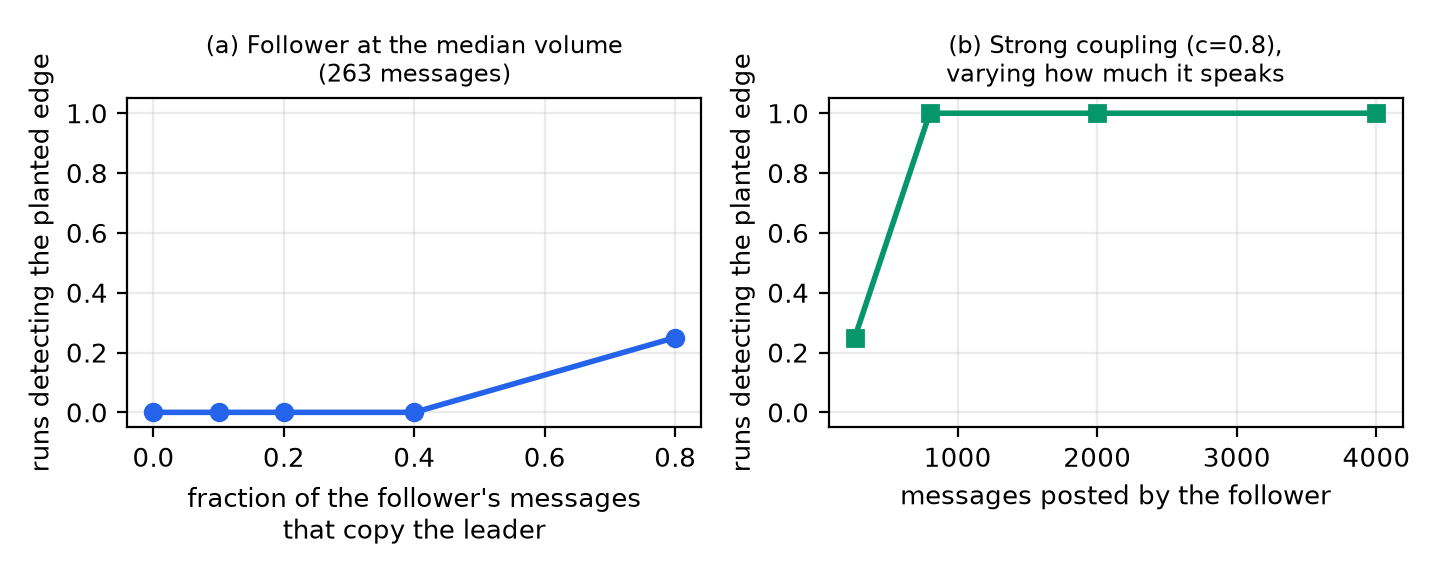
\includegraphics[width=0.92\textwidth]{f4_power.png}
\caption{Detection of a planted follower under the repaired surrogate. Left, varying the fraction of
its messages that copy the leader, at the median agent's volume. Right, varying how much it speaks,
at strong coupling.}
\end{figure}

\paragraph{Humans in the channel.} Main-village \#general is now effectively human-free, with 3 human
messages in the window, so the question has to be asked in open-chat, where 32\% of messages come
from 124 human visitors. Pairwise, with humans collapsed into one node, 19 edges are certified.
Conditioning removes almost all the agent-to-agent structure and little of the rest: \textbf{four
edges survive, of which three run from humans to agents, one is agent to agent, and none run from an
agent to a human.} The asymmetry is not an artifact of the confound. It should be read carefully all
the same: topical dependence from a person to an agent is also what ordinary responsiveness looks
like, so the measurement supports only that the dependence is dyad-specific and directional, not
that anyone is steering a swarm.

\section{Reproducibility, and one limitation of it}

Every number in this paper is recomputed from committed analysis output by a verifier that fails on a
mismatch, and that verifier covers the prose of this paper as well as the figures.

One limitation should be stated plainly. Re-running the counts in the earlier stationarity sweep with
the same seeds and configuration, only one of the eight cells reproduced exactly; the remaining
differences were one or two replicates per cell. Seven of the eight published rates still fell within
the recomputed Wilson intervals, and no conclusion changed. The exception is the zero-drift cell under
the permutation null, where the published 1 of 30 falls just below the recomputed interval of
$[0.035, 0.256]$ for 3 of 30, and no result here depends on that cell.

The generator, estimator and BLAS configuration were investigated and ruled out as the source. The
most likely explanation is a library-level difference, particularly in scikit-learn's $k$-means
implementation within the symboliser, whose output can vary between versions. Every sweep now records
the environment it ran under: Python 3.14.6, numpy 2.5.1, scipy 1.18.0 and scikit-learn 1.9.0,
including the BLAS build and the number of BLAS threads each worker used.

This does not make the previously published counts exactly reproducible. It provides a more clearly
specified environment in which subsequent results can be checked. For that reason I report rates
alongside their confidence intervals rather than exact replicate counts. The distinction between
reproducing a result within its uncertainty and reproducing every individual count matters, and only
the first is claimed.

\section{Conclusion}

Applied to real agent chat, the standard recipe for ``who drives whom'' needs repair before it says
anything. Clock windows cannot separate a message from its answer at the speed agents reply, and what
they certify is matched by a null with no access to meaning. The turn-ordered grid that fixes this
breaks the circular-shift surrogate: family-wise error 0.90 against a nominal 0.05, caused by the
speaker sequence itself. Restricted permutation surrogates repair most of that, but they are flat
under drift rather than calibrated, they are mutually indistinguishable at this precision, and one of
them needs twice the surrogate draws anyone would think to use. A valid surrogate fixes calibration
but not confounding. What survives is small: two dyad-specific edges that do not replicate, an
undetermined answer set by conditioning resolution, and influence running from people into agents and
never back. \textbf{An influence graph should not guide decisions until its error rate, its confound,
its detection floor and its symboliser's fidelity are reported.}

\section*{Limitations}

\begin{itemize}
\item \textbf{Immediate-predecessor only.} The turn-ordered lag-1 measure sees influence from the
message directly before a reply. Influence acting over several turns, or through a room's accumulated
context, is out of scope.
\item \textbf{Discrete approximation to an event process.} Agent chat is event-based in continuous
time. The turn-ordered discretisation with a permutation surrogate is a practical fix, and the
continuous-time comparison above shows what that choice gives up.
\item \textbf{The mechanism behind the real 0.90 is not established.} The generator separates
turn-taking from drift and points at drift, but the largest cell anywhere in the design is 0.365.
\item \textbf{Symbolisation quality cannot be measured on the real logs.} The central result survives
an independent symboliser, but the edge count does not: it moves with alphabet size and with which
messages the topic model is fit on. The floor remains the largest unquantified threat.
\item \textbf{No ground truth in the real logs.} The validity argument rests on planted controls and
on the meaning-free null, not on recovering a known answer.
\item \textbf{Conditioning removes real influence too.} The conditional estimate discards influence
that works by shifting what the channel is talking about, which in a group chat may be a large part
of genuine influence. It is a lower bound on dyadic influence.
\item \textbf{The human result is exploratory.} It rests on one village and one window and should be
read as a lead.
\end{itemize}

\section*{Broader impact and ethics}

This work audits influence detection on a population of AI agents, which is dual-use. Used
defensively it helps an overseer decide what an influence graph is worth, and the main result is
deflationary: it tells practitioners to trust these outputs less, which reduces rather than increases
the chance of acting on a bad attribution. The same tooling could be used to identify the most
influential agent in a swarm in order to target it, or to surveil participants in a channel. Three
properties limit the misuse. The subjects are AI models; the dataset is already public under research
terms and no re-identification is added; and the measure is weak and local, recovering
immediate-predecessor topical dependence rather than any model of how to steer an agent.

The dataset's research terms were followed: research use only, no training on the data, no
re-identification, citation of the source, and notification of the authors of resulting publications.
Human participants appear only as an aggregate node or as anonymised visitor labels, never by name or
handle, and no content attributable to an individual person is reported. Message text and metadata
were read, never model weights or private user data.

The use of a large language model in this work is disclosed in the first-page footnote, as TMLR
requires.

\bibliographystyle{tmlr}
\bibliography{refs}

\end{document}
"               de-anonymised arXiv preprint
%   pdflatex "\def\TMLRMODE{accepted}% TMLR submission. Built 10 November 2026 from:
%   paper/00_PROSE_v1.md   the author's written sections, 78 figures auto-verified
%   report/REPORT_V2.md    the sprint report, every number recomputed by report/verify_v2.py
%
% ANONYMITY. \usepackage{tmlr} with no option is the anonymous submission mode: the tmlr
% package hides the author block itself. Switching to [preprint] de-anonymises for arXiv AND
% turns on the \ifpreprint branches below, which are the only places a name, a repository URL
% or the benchmark's distinctive name appears. So one source produces both documents and the
% anonymous build cannot leak an identifier that the preprint build adds.
%
% Build:  latexmk -pdf main.tex
\documentclass[10pt]{article}

% The mode is chosen at build time so that one source produces every variant and they cannot
% drift apart:
%   latexmk -pdf main.tex                                        anonymous TMLR submission
%   pdflatex "\def\TMLRMODE{preprint}% TMLR submission. Built 10 November 2026 from:
%   paper/00_PROSE_v1.md   the author's written sections, 78 figures auto-verified
%   report/REPORT_V2.md    the sprint report, every number recomputed by report/verify_v2.py
%
% ANONYMITY. \usepackage{tmlr} with no option is the anonymous submission mode: the tmlr
% package hides the author block itself. Switching to [preprint] de-anonymises for arXiv AND
% turns on the \ifpreprint branches below, which are the only places a name, a repository URL
% or the benchmark's distinctive name appears. So one source produces both documents and the
% anonymous build cannot leak an identifier that the preprint build adds.
%
% Build:  latexmk -pdf main.tex
\documentclass[10pt]{article}

% The mode is chosen at build time so that one source produces every variant and they cannot
% drift apart:
%   latexmk -pdf main.tex                                        anonymous TMLR submission
%   pdflatex "\def\TMLRMODE{preprint}\input{main}"               de-anonymised arXiv preprint
%   pdflatex "\def\TMLRMODE{accepted}\input{main}"               camera-ready
% Use build.py, which runs all of them and checks the anonymous output for leaks.
\providecommand{\TMLRMODE}{submission}
\makeatletter
\def\@tmlrpreprint{preprint}
\def\@tmlraccepted{accepted}
\ifx\TMLRMODE\@tmlrpreprint
  \usepackage[preprint]{tmlr}
\else
  \ifx\TMLRMODE\@tmlraccepted
    \usepackage[accepted]{tmlr}
  \else
    \usepackage{tmlr}
  \fi
\fi
\makeatother

\usepackage{hyperref}
\usepackage{url}
\usepackage{booktabs}
\usepackage{graphicx}
\usepackage{amsmath}

% Gate every identifying string on whether identity may be revealed at all. The flag to test is
% \if@accepted, NOT \if@preprint: tmlr.sty's [preprint] option sets BOTH, so \if@accepted is true
% for the preprint and the camera-ready and false only for the anonymous submission, which is
% exactly the condition wanted. Gating on \if@preprint alone also hid the repository URLs from the
% camera-ready, which is where this paper promises to give them. \if@accepted is internal to
% tmlr.sty, hence the \makeatletter. The anonymous build takes the second argument.
\makeatletter
\newcommand{\ifdeanon}[2]{\if@accepted#1\else#2\fi}
\makeatother
\newcommand{\benchname}{\ifdeanon{SwarmInfluence-Bench}{the benchmark}}

% An unmarked footnote, for the LLM-use disclosure. TMLR's FAQ requires the disclosure and names
% the location: authors must "mention explicitly in their submission that they have used this
% tool", "as a footnote on the first page". Verified against jmlr.org/tmlr/faq.html on 10 Nov 2026.
% It is therefore not optional, and it does not belong in Broader Impact, where it sat until now.
% Nothing in the policy asks for the vendor's name, so none is given.
\newcommand{\disclosurefootnote}[1]{%
  \begingroup\renewcommand\thefootnote{}\footnote{#1}\addtocounter{footnote}{-1}\endgroup}

\title{An Influence Graph Over AI Agents Certifies an Agent That Copies Nobody}

% Hidden by the tmlr package unless [accepted] or [preprint] is given.
\author{\name Manu Nicholas Jacob \email manunicholasjacob@gmail.com \\
        \addr Independent Researcher}

\def\month{11}
\def\year{2026}
\def\openreview{\url{https://openreview.net/forum?id=XXXXXXXXXX}}

\begin{document}
\maketitle

\begin{abstract}
Circular-shift surrogates can produce severely inflated false-positive rates when applied to
turn-ordered multi-agent conversations, reaching a family-wise error rate of 0.90 against a nominal
0.05. A generated benchmark separates two candidate mechanisms and points at non-stationary speaker
activity rather than turn-taking, which suppresses the failure rather than causing it. No setting of
either knob reproduces the observed 0.90, however, so what drives the full real-data failure remains
open. Restricted permutation surrogates substantially reduce the problem. Their error rate is flat
with respect to drift rather than at the nominal level, and for the global within-speaker variant it
depends on how many surrogate draws the null is built from. Calibration alone does not address
confounding, which motivates a conditional estimator validated against a benchmark with planted
ground truth. I also identify a symbolisation-dependent detection limit and develop label-free
diagnostics for it, and show that their calibration does not transport across degradation
mechanisms. The benchmark is released.
\end{abstract}

\disclosurefootnote{\textbf{Use of a large language model.} A large language model was used as an
assistive tool: to help write and run the analysis code, and to help draft this paper. The author is
responsible for every claim, number and figure. All results come from the released code run on the
public dataset, no result or reference is fabricated, and every number in this paper is recomputed
from committed analysis output by a verifier that fails the build on a mismatch.}

\section{Introduction}

When AI agents interact in a shared channel, it is useful to understand how they influence one
another. Information-theoretic methods offer a way to measure this through lagged transfer entropy,
surrogate testing, and per-agent influence scores. They are attractive because they require no
labels and no access to model internals, only a record of who said what and when. The reliability of
those measurements is what this paper examines.

Almost every demonstration of these detectors runs on synthetic traces with a planted leader, where
the analyst controls timing and vocabulary. Real agent chat is asynchronous, bursty, and written in
open language. The narrower question here is whether the standard recipe, applied to real agent
logs, returns anything an overseer should act on.

The audit runs on the AI Village corpus \citep{aidigest2026}, in which frontier models share chat
channels over eighteen months across four villages differing in size, lifetime and tempo, applying
the checks a reader should demand: planted controls, a meaning-free symboliser, replication in a
held-out window, and sensitivity to every parameter that had to be chosen.

\begin{enumerate}
\item The conventional circular-shift surrogate is \textbf{invalid} on turn-ordered agent chat: a
family-wise error rate of 0.90 against a nominal 0.05, caused by the structure of the speaker
sequence itself.
\item Restricted permutation surrogates restore most of the calibration, and re-certifying under one
\textbf{scrambles rather than shrinks} the answer: one channel loses all 11 of its edges, another
gains 15.
\item The three restricted variants are \textbf{mutually indistinguishable} at the precision reached
here, so the choice between them cannot be justified on error rate. The global within-speaker
variant additionally needs on the order of 200 surrogate draws, and over-fires by roughly a factor
of two at 100.
\item Calibration is not confounding, so a conditional estimate is added and validated on a released
benchmark with a known influence graph: common-cause false edges fall from 22.3 to 0.33, and on the
planted-edge instances precision rises from 0.17 to 0.80 with no loss of recall or power.
\item The same benchmark exposes a \textbf{symbolisation floor}. Below roughly 0.44 adjusted Rand
index between symboliser and truth, detection collapses whatever the estimator. Label-free
diagnostics detect that floor, but their calibration does not transport across degradation
mechanisms, and I report where it fails.
\item On the real channels two edges stand at every conditioning resolution, 18 are
\textbf{undetermined} between 0 and 13, none replicates out of sample, and what survives alongside
humans runs from people to agents.
\end{enumerate}

\section{Related work}

\paragraph{Transfer entropy and surrogates.} Transfer entropy \citep{schreiber2000} measures how much
a source's past reduces uncertainty about a target's next symbol beyond the target's own past.
Plug-in estimators are biased upward on short series, so significance rests on surrogate data, with
family-wise error controlled by a max-T test \citep{westfall1993}. The usual surrogate is a circular
time shift of the source.

\paragraph{Event-based data breaks the shift surrogate.} \citet{shorten2021}, on neural spike trains,
show that the conventional source-time-shift surrogate fails to represent the null hypothesis of
conditional independence for event-based processes, and adapt to that setting the nearest-neighbour
local permutation scheme of \citet{runge2018}. Agent chat is event-based in that sense: messages are
events in continuous time, not samples of a clocked signal. The correction is not a contribution of
this paper. The contribution is showing that the same failure carries over to multi-agent safety
monitoring, and that it can be severe enough to create apparent leaders where none exist.

\paragraph{The same failure, concurrently, in multi-agent reinforcement learning.}
\citet{papadopoulos2026} report a closely related surrogate failure in multi-agent
reinforcement-learning action series. Their agent pairs have zero influence by construction, yet
circular time shifts produce false-positive rates of 100\% and 98.2\% against a nominal 0.05. A
plain permutation surrogate fares no better in their setting, at 100.00\% and 99.95\%. Their
proposed correction restricts permutations to blocks of training time, which returns the rates to
5.25\% and 5.50\%.

There are important differences between their setting and this one. Their data consist of binary
actions recorded over twelve thousand training rounds, whereas these data are symbolised
natural-language messages arranged on a turn-ordered conversational grid. Their non-stationarity
comes from monotone drift associated with annealing exploration; here the relevant non-stationarity
appears in the speaker sequence. Neither result should be taken as a direct extension of the other.

Nevertheless, the fact that both approaches rely on restricted permutations is worth noting. Their
permutation blocks are defined by training time, while mine are defined by an agent's own speaking
positions. This provides convergent evidence that unrestricted temporal rearrangement can be
problematic in non-stationary multi-agent data. Their findings also serve as a useful warning for
the approach taken here, and the warning has a measured form rather than a rhetorical one: in their
data the unrestricted permutation failed as completely as the time shift, at 100.00\% against a
nominal 0.05. Permutation-based surrogates are not automatically protected against
non-stationarity, and what protects the one used here is the restriction, not the permutation. I
claim no priority over their result and view the two studies as complementary, addressing different
forms of structured multi-agent data.

\paragraph{Oversight under a budget.} AI-control research frames monitoring as resource constrained,
with a cost for false positives \citep{greenblatt2024}. An influence graph is one such measurement,
and its error rate is the concern here.

\paragraph{Clustering stability.} The idea of using clustering stability as a label-free quality
indicator is not new. It has a substantial history, including \citet{benhur2002},
\citet{lange2004}, von Luxburg's review of clustering stability \citep{vonluxburg2010}, and
\citet{tibshirani2005} on prediction strength. What is different in Section~\ref{sec:floor} is the
calibration of these diagnostics against a detection-performance floor rather than against cluster
recovery alone.

\section{Data and representation}

The AI Village dataset ships one gzipped-JSONL table per village. Four villages are used, differing
enough to test whether any finding is a property of one channel.

\begin{table}[h]
\centering
\begin{tabular}{lrrrrl}
\toprule
village & agent messages & agents & lifetime & human messages & busiest room \\
\midrule
main      & 205,726 & 58  & 576 days & 10,029 & \#general (166,715, 81\%) \\
open-chat &  35,483 & 23  &  66 days & 12,264 & \#general (all) \\
swarm     &   3,848 & 133 &   1 day  &      5 & room a (3,846) \\
game-jam  &     838 & 6   &   3 days &     36 & per-team rooms \\
\bottomrule
\end{tabular}
\caption{The four villages. A 2026 scaffolding change scopes each agent to its current room's
context, so the busiest room of each village is a self-contained influence substrate and is analysed
alone.}
\end{table}

The primary window is the final fourteen days of main-village \#general, 17 to 31 October 2026,
holding 8,800 agent messages. Twenty-two models posted at least 50 messages each and the directed
test uses the 15 busiest, giving 7,958 message events. Two scaffolding facts are disclosed rather
than corrected: the automated nudger was off throughout, and the unused \#best and \#rest rooms were
soft-deleted mid-window, which does not touch \#general.

\subsection{From open language to symbols}

Transfer entropy needs discrete symbols, so each message is mapped to a small alphabet before
influence is estimated, and that mapping is kept separate from the estimator. A topic symboliser
(TF-IDF then $k$-means, $k=8$) gives a message its topic cluster id, so paraphrases of one idea share
a symbol. A hash symboliser, a stable hash of the normalised text into $k=8$ buckets, has no notion
of meaning and serves as a null: an edge appearing under both lives in timing alone.

\subsection{The lag problem, and why clock windows cannot solve it}

A lag-1 transfer entropy compares window $t-1$ with window $t$, so influence landing inside one
window is invisible to it. Agent chat makes this binding. Among the fifteen analysed agents the gap
between consecutive messages by different speakers has a median of 28.1 seconds (25th percentile
9.2, 75th 66.2, 95th 159.3), so turn-taking is a seconds-scale process while any clock window wide
enough to hold two speakers is minutes wide and swallows both a message and its answer.

Both horns are measurable. At 30 seconds only 1.2\% of agent-windows hold a message, while 32.0\% of
replies already land in the same window as what they answer, rising to 84.4\% at five minutes. At
every width tried, the meaning-free hash null certifies comparably many edges, and more at five
minutes: 9 against 12 at thirty seconds, 17 against 19 at one minute, 27 against 44 at fifteen, and
19 against 17 at five. Whatever clock-window transfer entropy was detecting there, it was not shared
meaning.

\begin{figure}[h]
\centering
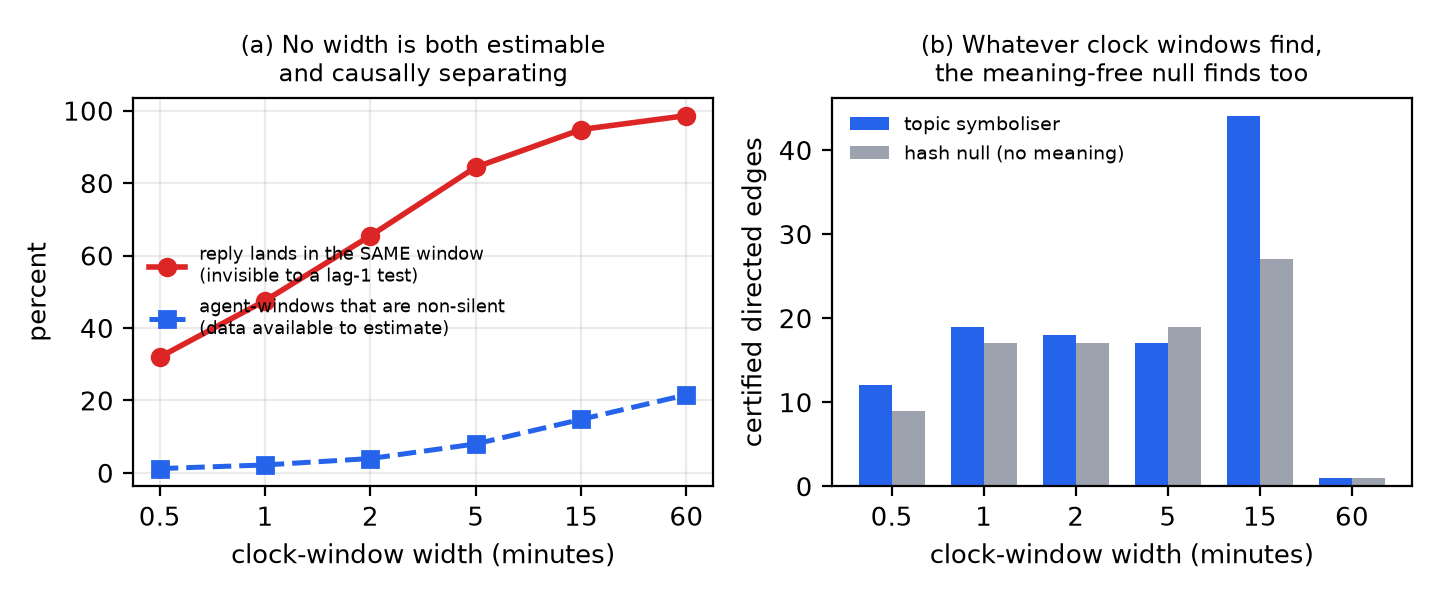
\includegraphics[width=0.92\textwidth]{f1_clock.png}
\caption{Clock-window transfer entropy on the 15 analysed agents of main-village \#general. Left,
the two failure modes as a function of window width. Right, edges certified under the topic
symboliser against the meaning-free hash null.}
\end{figure}

The bind is avoided by ordering messages canonically and letting one message be one tick. Each
agent's series carries its symbol where it spoke and a silent symbol elsewhere, so the lag-1
comparison is between a message and the one immediately before it. The cost is that the measure
captures immediate-predecessor influence only.

\section{The surrogate failure, and two explanations that did not hold}
\label{sec:failure}

An agent is planted into the real stream, drawing its symbols from the channel's marginal and
coupled to nothing at all. It is certified as driving something in 3 of 8 runs when it posts 50
messages, and in 8 of 8 at 100, 263, 600 and 1500 messages, with the mean largest $z$ rising from 5.6
to 12.3, 21.7, 38.3 and 71.7. The error grows with how much the agent speaks, which rules out a
small-sample explanation.

A planted agent could be dismissed as artificial, so the error rate is also measured directly.
Keeping the real speaker sequence and permuting the symbols globally leaves data with no directed
topical influence by construction. The shift surrogate certifies at least one edge in 9 of 10 such
replicates, a family-wise error rate of 0.90 against a nominal 0.05.

\paragraph{What breaks it is the speaker sequence.} Destroying one structure at a time isolates the
cause. Keeping the real speaker order and shuffling only symbols, the shift surrogate fires in 10 of
10 replicates; randomising the speaker order as well drops it to 0 of 10; uniform symbols with the
real order still give 6 of 10. So the driver is the structure of the speaker sequence, not the
symbol distribution and not sparsity. That sequence is far from random in two ways at once: it
repeats a speaker 36\% of the time and returns after one message 38\% of the time, and each agent's
activity is strongly non-stationary, with a median block-share coefficient of variation of 0.79.
Shuffling the order destroys both at once, so this ablation cannot say which of the two mattered.

\subsection{Two explanations I proposed, and the benchmark refuted both}

I initially attributed the failure to mutual exclusivity: only one agent can speak at each tick, so
shifting individual timelines could create overlaps that never occurred in the original
conversation. The benchmark did not support this explanation. A generated channel with exactly one
speaker per tick and steady activity produced an error rate of just 0.025, 95\% Wilson
$[0.011, 0.057]$, far below the 0.90 observed in the real data. Mutual exclusivity alone therefore
cannot explain the failure.

I then suspected turn-taking. In the real channel, speakers repeat 36\% of the time and return after
exactly one message 38\% of the time. However, adding a Markov speaker chain to the generator
produced the opposite result. Turn-taking suppressed the error rather than increasing it. At the
nominal knob values and with no drift the surrogate certified nothing at all across 200 replicates,
while removing turn-taking and introducing drift raised the rate to 0.365. The contribution from
drift was $+0.340$, compared with $-0.025$ for turn-taking. The same inversion appears in the arm
calibrated so that the generated channel reproduces the real channel's measured repeat, return and
block-share statistics rather than merely carrying those numbers as settings: there, turn-taking
alone also certifies nothing, and drift alone gives 0.065.

Neither mechanism, nor their combination in the tested design, reproduced the real-data error rate of
0.90. The largest cell anywhere in the design is 0.365. The real-data ablation removes turn-taking
and non-stationarity together, while the generator separates them. The results point to
non-stationary activity, but the remaining gap means the mechanism behind the full real-data failure
is not yet established.

Every figure above comes from the run at 200 surrogate draws. The first version of this analysis
used 100, which inflates both nulls on the same 2,400 instances: the circular shift fires 53 times
where the 200-draw run does not, against 18 the other way (exact McNemar $p = 3.9 \times 10^{-5}$),
and the permutation surrogate 83 against 20 ($p = 2.7 \times 10^{-10}$). Every qualitative conclusion
in this section is the same at both settings, which is why they are worth stating at all. The
numbers are not, so the draw count belongs in the caption.

\section{The repair, compared}
\label{sec:repair}

Following the local-permutation idea of \citet{runge2018} as adapted by \citet{shorten2021}, each
source keeps its speaking positions and only its symbols are permuted among them. Speaking pattern,
sparsity and turn-taking are preserved exactly, and only the correspondence between symbol and time
is destroyed. On the same destroyed-structure real data the family-wise error rate falls to 0.063
over 300 replicates, 95\% Wilson $[0.041, 0.097]$. The planted uncoupled agent is never certified: 0
of 5 at both 263 and 1500 messages, with mean max $z$ of 2.8 in each case against 22.0 and 68.3
under the shift surrogate.

\begin{figure}[h]
\centering
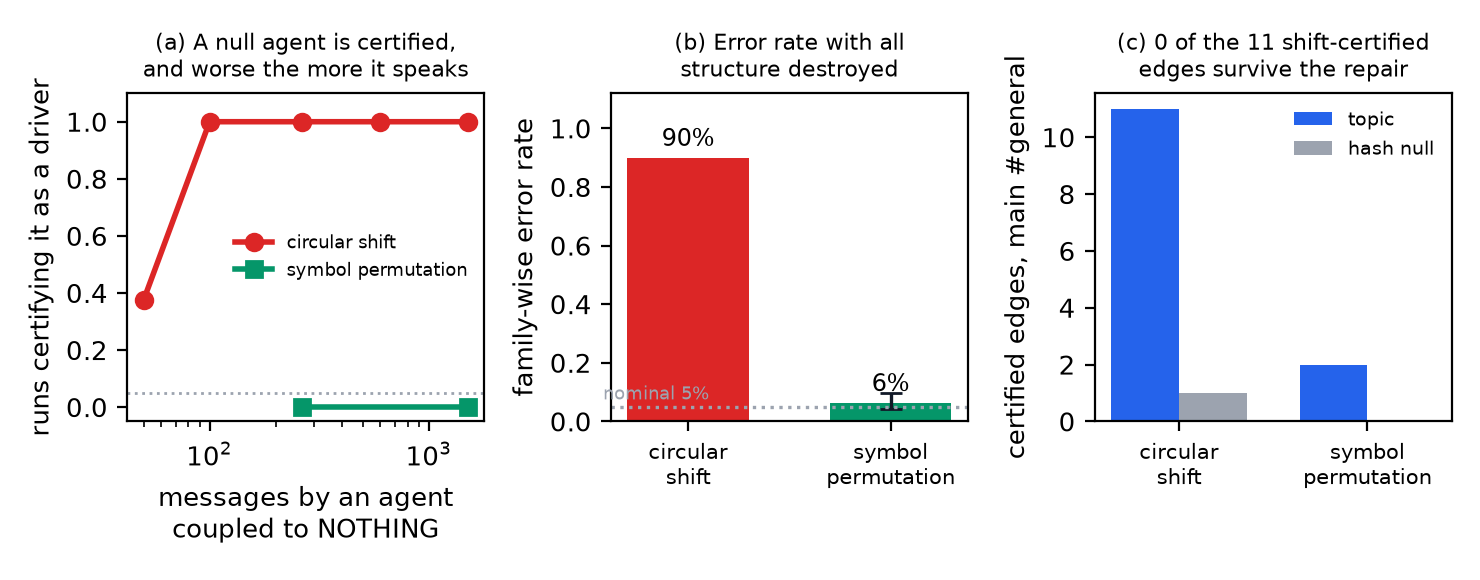
\includegraphics[width=\textwidth]{f2_null.png}
\caption{Left, how often an agent coupled to nothing is certified as a driver, under each surrogate.
Middle, family-wise error rate measured on data with all structure destroyed, with a Wilson
interval; the dotted line is the nominal 0.05. Right, what each surrogate certifies on the real
channel.}
\end{figure}

\subsection{How many surrogate draws are needed}

The number of surrogate draws matters more than I initially appreciated. In a paired comparison of
300 instances, where all four surrogates run on identical symbol grids so the outcomes are paired,
the global permutation surrogate produced a false-positive rate of 0.1167 with 100 draws, falling to
0.0700 with 200 draws, 95\% Wilson $[0.046, 0.105]$. This difference is statistically significant
(exact McNemar $p = 0.0043$). The block-local and Runge local permutations were less sensitive to the
increase: their corresponding rates changed from 0.0900 to 0.0767 and from 0.0967 to 0.0800.

At 200 draws, the global permutation's interval covers the nominal 0.05 and overlaps the real-data
estimate of 0.0633 $[0.0409, 0.0968]$. The real-data result is therefore corroborated rather than
overstated. For practical use, the important point is that reducing the number of surrogate draws
can materially change the result. In particular, the global permutation over-fires at 100 draws by
approximately a factor of two. I would therefore not treat the choice of draw count as a minor
computational detail.

The same correction applies to the benchmark-wide estimate. That figure was 0.0942 at 100 draws.
Repeating all 2,400 instances at 200 draws gives \textbf{0.0679}, 95\% Wilson $[0.0585, 0.0787]$,
and the paired difference is large: 83 instances fire at 100 draws and not at 200, against 20 the
other way, $p = 2.7 \times 10^{-10}$. The conclusion it supports is unchanged, because the interval
still excludes the nominal 0.05. So the permutation repair does carry a residual inflation on clean
generated data, but it is about a third above nominal rather than nearly double.

One limit on this recommendation. I compared 100 draws against 200 and did not test any larger
value, so what the experiment establishes is that 100 is too few, not that 200 is enough. Two
hundred is a lower bound on the draw count rather than a converged setting, and a practitioner whose
conclusions sit near a decision boundary should check their own sensitivity rather than adopt the
number.

\subsection{Choosing a repair, when the error rate cannot choose}

The comparison of the three permutation-based repairs does not produce a clear winner. All four
surrogates were evaluated on identical symbol grids across 300 pure-null replicates, so the
comparison reflects differences between the null models rather than differences between datasets.

\begin{table}[h]
\centering
\begin{tabular}{lrrrl}
\toprule
surrogate & FWER, 100 draws & FWER, 200 draws & 95\% Wilson at 200 & nominal 0.05 \\
\midrule
circular shift                   & 0.0433 & \textbf{0.0333} & $[0.018, 0.060]$ & inside \\
global within-speaker permutation & 0.1167 & \textbf{0.0700} & $[0.046, 0.105]$ & inside \\
block-local permutation          & 0.0900 & \textbf{0.0767} & $[0.052, 0.112]$ & excluded \\
local permutation \citep{runge2018} & 0.0967 & \textbf{0.0800} & $[0.054, 0.116]$ & excluded \\
\bottomrule
\end{tabular}
\caption{Four surrogates on identical symbol grids, 300 pure-null replicates, at both draw counts.}
\end{table}

At 200 draws, paired on the same 300 instances, the circular shift is not significantly different
from the global permutation ($p = 0.0614$), although it differs from block-local permutation
($p = 0.0294$) and from Runge's local permutation ($p = 0.0201$). At 100 draws it differed from all
three, which is the draw-count artifact again. The three repairs remain statistically
indistinguishable from one another, with pairwise $p$-values of 0.85, 0.65 and 1.00. The apparent
differences in their error rates are not sufficient to establish a ranking.

Choosing between them therefore requires more than calibration, and two readings pull against each
other. Runge's local permutation has the strongest methodological justification for preserving the
structure it is intended to preserve, and it follows the approach adapted to event data by
\citet{shorten2021}. Block-local permutation is more heuristic and introduces a free parameter that
has not been tuned. Global permutation is the simplest. On the other hand, the global permutation has
the most favourable interval relative to the nominal rate, and is the only repair that costs nothing
measurable against the shift on clean stationary data, although neither difference is statistically
established. I do not consider the observed error rates sufficient to select one repair over the
others. The choice should be guided by the structure the null is intended to preserve and the
assumptions that can be justified for the data.

\subsection{When to use the repair}

A drift sweep gives the practical reading. Across 150 replicates per cell at 200 surrogate draws,
the circular shift degrades steadily as activity drift increases while the three repairs do not.

\begin{table}[h]
\centering
\begin{tabular}{lrrrr}
\toprule
activity drift & circular shift & global permutation & block-local & local \\
\midrule
0.0 & \textbf{0.013} & 0.093 & 0.080 & 0.093 \\
0.3 & 0.100 & 0.100 & 0.093 & 0.120 \\
0.6 & \textbf{0.193} & 0.053 & 0.047 & 0.067 \\
0.9 & \textbf{0.380} & 0.087 & 0.080 & 0.080 \\
\bottomrule
\end{tabular}
\caption{Family-wise error on pure nulls as activity drift increases, 150 replicates per cell, 200
surrogate draws. Every certified edge is a false positive by construction.}
\end{table}

The pattern is supported by a formal trend test rather than by eye. A Cochran-Armitage test across
the four ordered drift levels gives the circular shift $z = 8.667$, $p < 10^{-15}$, and gives every
repair nothing: $p = 0.51$ for the global permutation, 0.63 for block-local and 0.37 for local. The
same pattern holds at both surrogate draw counts, so it does not depend on that choice.

The repairs are therefore flat under drift rather than calibrated. Only one of the four global
permutation intervals covers the nominal 0.05, and the rest sit nearer 0.09, so what the repair buys
is insensitivity to drift rather than correctness. One asymmetry should be stated rather than
hidden: block-local covers nominal in three of the four cells where the global repair covers one.
The two remain pairwise indistinguishable, so this is not grounds to switch the recommendation, but
it does mean the global repair cannot be described as the best-calibrated under drift.

The results also show why the repair should not be treated as universally preferable. At zero drift
the circular shift has an error rate of 0.013, while the three repairs are all around 0.08 to 0.09.
That advantage is gone by the first drift step: at drift 0.3 the shift reads 0.100 against the global
permutation's 0.100 and block-local's 0.093, so the crossover falls between drift 0.0 and 0.3 rather
than at some higher level. By drift 0.6 the shift is roughly four times the repairs. If a channel has
been checked and found stationary, the circular shift may be sufficient. When activity is
non-stationary the repairs are the more stable choice, and the margin for error on that judgement is
narrow, because the crossover arrives by the first drift level tested.

\section{Continuous time, and what the repair cannot test}

An earlier analysis identified continuous-time estimation as the principled option for event data
but did not evaluate it. Running the continuous-time estimator CoTETE on both channels certifies 0
edges in either case, compared with 2 for main-village and 18 for open-chat under the discrete,
turn-ordered analysis. Its highest $z$-scores are 3.062 and 3.980, below the respective max-T
thresholds of 4.171 and 4.308.

At first these results might appear to contradict the symbol-based analysis. The two estimators
operate on different information, however. CoTETE's public API takes event times with no symbol
channel, while the transfer-entropy analysis here uses topic symbols. To test whether this
difference explains the results, I reduced the data to timing alone, replacing every spoken symbol
with the same code. Under this representation the estimator used here also detects 0 edges in both
channels, matching CoTETE. Using the circular-shift surrogate instead produces 12 and 3 edges. So
neither method detects relationships from event timing alone in these channels, and the edges found
by the symbol-based analysis depend on symbol correspondence, which the continuous-time estimator
cannot access.

Two caveats attach to those $z$-scores, and the second attaches to the larger of them. Point
estimates from this estimator are stochastic to about 17\% across repeated runs, so none of these
values should be read to more than two significant figures. And open-chat's highest $z$, the 3.980,
belongs to the one pair whose surrogate draws mostly failed: it needed 1,936 failed draws to obtain
100 successes, a 4.9\% success rate. Those surrogates are conditioned on being estimable, so that
pair's null is biased in an unknown direction. The conclusion does not rest on it, since that pair
falls below threshold and so does every other pair, but the number should not be quoted as a clean
measurement. The failures themselves were a defect rather than a property of the data: an enlarged
exclusion window can empty the neighbour search on sparse bursty event trains and raise an error
that terminates a whole pair, with no handling at the public entry point. This has been reported
upstream.

There is also a fundamental limitation in applying the recommended permutation surrogate to
timing-only data. When every event carries the same symbol, permuting those symbols changes nothing.
The observed statistic and the surrogate null are identical, making the test exactly degenerate:
standard deviation 0 across all 210 pairs and $p = 1.0$ everywhere. \textbf{The repair has zero power
against timing structure by construction.} The permutation surrogate is appropriate for testing
relationships in the symbol sequence, but it does not answer whether relationships exist in event
timing. These are different questions, and choosing one null means giving up the ability to test the
other with that procedure.

\section{Confounding, and what conditioning removes}

A valid surrogate fixes calibration but not confounding. If every agent tracks a drifting channel
topic, every pair is genuinely dependent through the channel, and pairwise transfer entropy cannot
tell that from direct influence. I therefore also report a \textbf{conditional} estimate, which asks
whether a source's last message adds anything about a target's next one beyond the target's own
history and the channel's recent state. The conditioning variable is the modal symbol of the last
twelve messages, excluding the immediately preceding one so that it does not simply restate the
source.

On a generated benchmark whose decisive instances contain no influence while every agent tracks a
shared drifting topic, so that any certified edge is common cause, pairwise transfer entropy
certifies \textbf{22.3} edges on average and conditioning takes that to \textbf{0.33}, lifting pooled
precision on the four-edge instances from 0.17 to \textbf{0.80} at a recall of 1.0 either way. Across
couplings from 0.05 to 0.8 the conditional test still finds the planted edge in 3 of 3 runs, so the
gain costs no power.

The benchmark flatters the conditional estimator, since its common cause is a shared modal topic and
the conditioning variable is the channel's modal topic. The real channels are harder, and
conditioning there costs degrees of freedom: a 9-symbol alphabet with a 9-valued context gives 6,561
cells against about 7,900 ticks, so that variable is also coarsened to 4 and 2 values.

\begin{table}[h]
\centering
\begin{tabular}{lrrrr}
\toprule
channel & pairwise & conditional, 9 values & 4 values & 2 values \\
\midrule
main \#general      & 2  & \textbf{2, the same two edges} & 2 & 3 \\
open-chat \#general & 18 & \textbf{0} & \textbf{7} & \textbf{13} \\
swarm, room a       & 1  & \textbf{0} & & \\
\bottomrule
\end{tabular}
\caption{Conditioning at three resolutions. Main-village's two edges are robust to that choice;
open-chat's zero is not.}
\end{table}

At the finest resolution the open-chat test is degenerate, its surrogate sitting above the observed
statistic for 65\% of pairs with the largest $z$ in the family only 4.4, so it is failing to reject
rather than finding nothing to reject. Open-chat's structure therefore remains
\textbf{undetermined}: depending on the conditioning resolution, between 0 and 13 of its 18 edges may
survive. That resolution is a free parameter an analyst would set once and never revisit. This is a
property of the channel rather than the estimator: on structure-free real data the conditional test
fires in 2 of 40 replicates, an error rate of 0.05 with a mean $z$ of $-0.001$, so it is nominal
rather than conservative.

\section{The symbolisation floor}
\label{sec:floor}

Everything these methods produce is downstream of turning text into symbols. On the benchmark, where
the underlying topics are known, detection performance drops sharply when agreement between the
symboliser and the ground truth falls below roughly ARI 0.44, and this behaviour appears across the
tested estimators. Importantly, the false-positive rate can look \emph{better} below this point,
because the shared topic structure needed to produce confounded detections is no longer represented
reliably. A pipeline that stops detecting relationships may therefore have lost the signal it needs
rather than become more reliable, and nothing downstream of the symboliser can tell those apart.

\subsection{Detecting the floor without labels}

That degradation can be detected without ground-truth labels. Across the nine-level benchmark sweep,
three statistics separate the below-floor cases with zero errors: seed stability at a threshold of
0.623, agreement with LSA at 0.646, and the Calinski-Harabasz index at 138.9. Seed stability here is
the \textbf{minimum} pairwise agreement across seeds, not the mean; the mean variant makes one error,
at a different threshold of 0.791. Silhouette has the strongest correlation with true ARI, at 0.979,
but is not useful for identifying the boundary because its threshold falls within a gap of just
0.002. A statistic that tracks clustering quality most closely is not necessarily the best one for
making a classification decision.

Error count cannot choose among the three that were perfect, so I tested whether each threshold still
means what it meant when the channel changes for reasons other than topic separability. Applying each
cut unchanged to thirty cells that vary turn-taking, drift, agent count, volume skew, message length
and corpus size, twenty-seven of which hold true ARI at exactly 1.000:

\begin{table}[h]
\centering
\begin{tabular}{lrrrr}
\toprule
diagnostic & cut & errors where fitted & errors, nuisance set & of those at true ARI 1.000 \\
\midrule
seed stability, min across seeds & 0.623 & 0 & 2 & \textbf{0} \\
LSA agreement                    & 0.646 & 0 & 2 & \textbf{0} \\
Calinski-Harabasz                & 138.9 & 0 & 6 & \textbf{3} \\
\bottomrule
\end{tabular}
\caption{Whether a cut fitted on the vocabulary-overlap mechanism survives a change in the channel
that is not a change in topic separability.}
\end{table}

The two bounded statistics err only on the short-message cells, where the symbolisation genuinely has
degraded. Calinski-Harabasz additionally condemns all three cells whose true ARI is exactly 1.000,
for no reason beyond the corpus holding 2,000 messages rather than 8,000, where it reads 76 to 77
against its own cut of 138.9. It is unbounded and grows with sample size, so a published numeric
threshold for it carries no meaning on another corpus. That is why I recommend the two bounded
statistics and not the index that matched them on error count. \textbf{A cut that moves with the
corpus is not a floor cut.}

This is not a weak statistic being discarded on a technicality. Calinski-Harabasz correlates with
true ARI at 0.973, almost as closely as silhouette, and unlike silhouette it classifies the floor
perfectly where it was fitted. It still cannot carry a published threshold. That is the sharper form
of the point above: neither the statistic that tracks quality most closely nor the one that
classifies best on the fitting mechanism is necessarily the one whose cut another researcher can
reuse.

There are important limits to this result. The effective sample size is nine rather than 54, because
the classification label is determined by overlap level. There are no observations between ARI 0.444
and 0.222, so the exact location of the boundary within that interval remains unknown. These
diagnostics classify whether a result is below the tested detection floor; they do not estimate ARI,
and their behaviour is flat between 0.68 and 1.00, and not even monotone there. The benchmark also
uses a single degradation mechanism with a known and correct value of $k$, whereas the true number of
topics in real conversations is unknown. I therefore treat 0.44 as a benchmark-specific, bracketed
result rather than a universal threshold.

\subsection{A contradiction the diagnostic lost}

I initially used these diagnostics to classify one real channel, open-chat, as below the
symbolisation floor. That conclusion did not agree with the channel's measured results: open-chat
certified 18 and 22 edges under the two symbolisers, compared with 2 and 1 for main-village, and its
hash-based null certified zero edges. Rather than treating this disagreement as evidence that the
original measurements were wrong, I revisited the diagnostic itself.

The problem was the choice of $k$. Repeating the comparison with the same channels, loader and window
reproduced the published $k=8$ results to the digit. At $k=4$, however, open-chat reached stability
scores of 0.950 and 0.978, the highest values produced by either channel across the tested settings,
and both exceeded the diagnostic thresholds. The earlier below-floor classification was therefore a
conclusion about one arbitrary choice of $k$, not a reliable statement about the channel. Message
length does not explain the difference either: 27.1\% of main-village messages contain fewer than
five tokens, compared with 2.3\% in open-chat, so the short-message channel is the one the diagnostic
cleared.

This correction changes how the symbolisation results should be read, and it withdrew three claims.

\begin{enumerate}
\item \textbf{The claim that no topic signal remains below the floor is too strong.} The
circular-shift surrogate recovers all four planted edges at every tested overlap level, including
0.95, where ARI is 0.011. The observed collapse is in the permutation null, not necessarily in the
underlying data.
\item \textbf{ARI 0.44 cannot be treated as a universal detection threshold.} When the shared-topic
parameter is 0, detection continues down to ARI 0.296, so the boundary depends on both the
symboliser and the channel.
\item \textbf{Edge counts cannot be used as a measure of symboliser quality.} Even at ARI exactly
1.000, changing the shared-topic parameter alone moves the permutation edge count from 5 to 78.
\end{enumerate}

The diagnostics also do not transfer reliably outside the mechanism on which they were evaluated.
Their balanced accuracy falls from 1.00 to 0.75 and 0.571 under a known mismatch in $k$. All seven
errors made by seed stability are false below-floor classifications, and in every one of those cases
the detector still identifies all planted edges; of the fourteen cells it condemned, eleven had full
conditional recall. The failure direction is the dangerous one: it condemns working symbolisations.

This was an important correction to my own interpretation. I introduced a diagnostic to check whether
the symbolisation was reliable, applied it to the real channels, and found that it contradicted
measurements already in hand. Investigating that contradiction showed the diagnostic was sensitive to
an arbitrary modelling choice. The result is not that the original measurements were wrong, but that
the control was being asked to support a broader conclusion than the evidence allowed. These
diagnostics remain useful within their tested setting, and \textbf{no channel-level floor verdict
should be issued from a single $k$}.

\section{The benchmark}

Real logs have no ground truth, so the common-cause question could not be settled on them. The
generator used here makes the influence graph known by construction: it decides, in code, who speaks
at which tick, on which topic, and who reacts to whom. Surface text is a separate, replaceable layer
drawn from disjoint per-topic vocabularies, so the whole thing runs offline and a detector still has
to symbolise raw text rather than read the labels. Turn-taking and activity drift are independent
knobs, so the two can be varied one at a time, and the generator reproduces its earlier behaviour
bit for bit when both are zero.

\benchname{} is released with 150 tests covering the generator, the detector harness, the text layer,
the floor analysis and the turn-taking factorial.
\ifdeanon{Code and benchmark:
\url{https://github.com/manunicholasjacob/swarm-influence-bench} and
\url{https://github.com/manunicholasjacob/swarm-influence-audit}.}{Code and benchmark are publicly
released; the links are withheld here for anonymity and will be given in the camera-ready version.}

One property of the benchmark must be stated when its numbers are quoted. Planting an edge displaces
other agents' speaking turns, so the generated instances contain real lag-1 dependencies that the
label set does not list. Precision measured against those labels is therefore a \textbf{lower bound}
for any detector, and what the benchmark supports is the comparison between two estimators rather
than the absolute value of either.

\section{What an overseer should do}

Six inexpensive controls should be included whenever an influence graph over an agent channel is
published.

\begin{enumerate}
\item \textbf{Plant an agent coupled to nothing, at your channel's volumes, and check it is not
certified.} This one test would have caught the failure reported here, at one run per volume.
\item \textbf{Measure the error rate directly}, by destroying the structure your method claims to
find and checking the family-wise rate is near nominal. If it is not, your surrogate does not match
your data.
\item \textbf{Preserve the speaker sequence in your surrogate.} Any surrogate that moves an agent's
messages in time will disturb it, and \citet{shorten2021} is the principled route. Use at least 200
surrogate draws, because at 100 the global within-speaker permutation over-fires by roughly a factor
of two.
\item \textbf{Establish the detection floor before interpreting an absence.} ``No edges'' and ``no
influence'' are different claims.
\item \textbf{Condition on the channel, report both numbers, and sweep the resolution.} Pairwise and
conditional bound the answer, and the gap between them is the result. Conditioning costs cells, so
check whether your answer is an artifact of how finely you conditioned. On one channel here it was.
\item \textbf{Report how well your symboliser agrees with the truth, on data where you know it.}
Everything is downstream of turning text into symbols, and below roughly ARI 0.44 detection
collapses whatever the estimator. I have found this control in no influence-detection paper, and it
is also the one that cannot be run on real logs, which is why the floor remains the largest
unquantified threat here.
\end{enumerate}

Two habits follow: publish a meaning-free null's count beside the real one, and require held-out
replication before calling a graph a structure.

\section{The real channels, and what survives}

Re-running every channel under the repaired surrogate changes the answers, and not in one direction.

\begin{table}[h]
\centering
\begin{tabular}{lrrr}
\toprule
channel & window messages & shift: topic / hash & permutation: topic / hash \\
\midrule
main \#general      & 8,800 & 11 / 1 & 2 / 0 \\
open-chat \#general & 8,226 & 3 / 0  & 18 / 0 \\
swarm, room a       & 3,846 & 2 / 1  & 1 / 0 \\
\bottomrule
\end{tabular}
\caption{The same channels under both surrogates, with the meaning-free hash null beside each.}
\end{table}

In main-village, \textbf{none} of the 11 edges the standard recipe certifies survives the repair, and
the two the valid surrogate certifies were not among them. In open-chat the correction runs the other
way, 3 edges becoming 18, because pathological pairs inflate the max-T threshold and raise the bar
for everything else. An invalid surrogate does not simply add false positives; it scrambles the
result.

Main-village's two edges are the strongest thing here and they are still not a finding, because they
do not replicate: the adjacent fourteen-day window certifies nothing at all under either estimator.
Given the detection floor, that silence is as consistent with the test sitting near its limit as with
the edges being absent, and the two cannot be separated. Power is governed by how much an agent says
as much as by how strongly it copies, and it is channel-specific: in main-village a planted follower
copying on 80\% of its messages is caught only 1 time in 4, while in open-chat one copying 10\% of
the time is caught 3 times in 4. Replication is weak everywhere: under the standard recipe the
adjacent window shares 1 edge out of 8 and 4, and that edge is also the only one the hash null
certifies. No certified edge in this work replicates out of sample.

\begin{figure}[h]
\centering
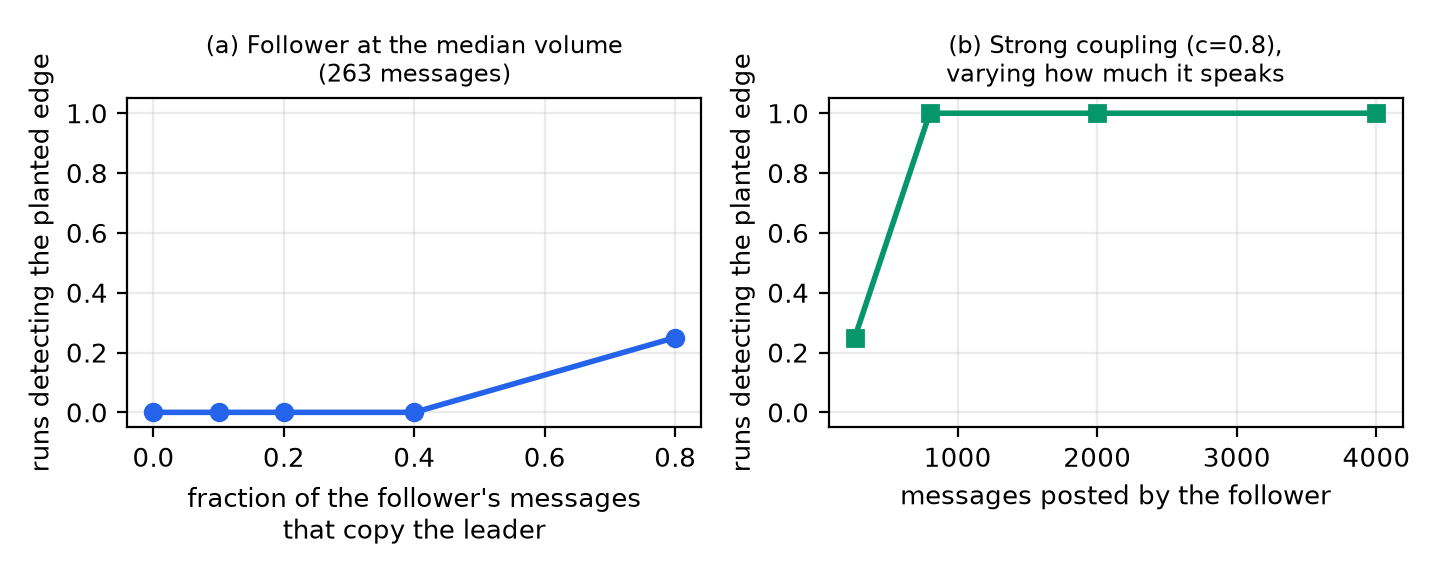
\includegraphics[width=0.92\textwidth]{f4_power.png}
\caption{Detection of a planted follower under the repaired surrogate. Left, varying the fraction of
its messages that copy the leader, at the median agent's volume. Right, varying how much it speaks,
at strong coupling.}
\end{figure}

\paragraph{Humans in the channel.} Main-village \#general is now effectively human-free, with 3 human
messages in the window, so the question has to be asked in open-chat, where 32\% of messages come
from 124 human visitors. Pairwise, with humans collapsed into one node, 19 edges are certified.
Conditioning removes almost all the agent-to-agent structure and little of the rest: \textbf{four
edges survive, of which three run from humans to agents, one is agent to agent, and none run from an
agent to a human.} The asymmetry is not an artifact of the confound. It should be read carefully all
the same: topical dependence from a person to an agent is also what ordinary responsiveness looks
like, so the measurement supports only that the dependence is dyad-specific and directional, not
that anyone is steering a swarm.

\section{Reproducibility, and one limitation of it}

Every number in this paper is recomputed from committed analysis output by a verifier that fails on a
mismatch, and that verifier covers the prose of this paper as well as the figures.

One limitation should be stated plainly. Re-running the counts in the earlier stationarity sweep with
the same seeds and configuration, only one of the eight cells reproduced exactly; the remaining
differences were one or two replicates per cell. Seven of the eight published rates still fell within
the recomputed Wilson intervals, and no conclusion changed. The exception is the zero-drift cell under
the permutation null, where the published 1 of 30 falls just below the recomputed interval of
$[0.035, 0.256]$ for 3 of 30, and no result here depends on that cell.

The generator, estimator and BLAS configuration were investigated and ruled out as the source. The
most likely explanation is a library-level difference, particularly in scikit-learn's $k$-means
implementation within the symboliser, whose output can vary between versions. Every sweep now records
the environment it ran under: Python 3.14.6, numpy 2.5.1, scipy 1.18.0 and scikit-learn 1.9.0,
including the BLAS build and the number of BLAS threads each worker used.

This does not make the previously published counts exactly reproducible. It provides a more clearly
specified environment in which subsequent results can be checked. For that reason I report rates
alongside their confidence intervals rather than exact replicate counts. The distinction between
reproducing a result within its uncertainty and reproducing every individual count matters, and only
the first is claimed.

\section{Conclusion}

Applied to real agent chat, the standard recipe for ``who drives whom'' needs repair before it says
anything. Clock windows cannot separate a message from its answer at the speed agents reply, and what
they certify is matched by a null with no access to meaning. The turn-ordered grid that fixes this
breaks the circular-shift surrogate: family-wise error 0.90 against a nominal 0.05, caused by the
speaker sequence itself. Restricted permutation surrogates repair most of that, but they are flat
under drift rather than calibrated, they are mutually indistinguishable at this precision, and one of
them needs twice the surrogate draws anyone would think to use. A valid surrogate fixes calibration
but not confounding. What survives is small: two dyad-specific edges that do not replicate, an
undetermined answer set by conditioning resolution, and influence running from people into agents and
never back. \textbf{An influence graph should not guide decisions until its error rate, its confound,
its detection floor and its symboliser's fidelity are reported.}

\section*{Limitations}

\begin{itemize}
\item \textbf{Immediate-predecessor only.} The turn-ordered lag-1 measure sees influence from the
message directly before a reply. Influence acting over several turns, or through a room's accumulated
context, is out of scope.
\item \textbf{Discrete approximation to an event process.} Agent chat is event-based in continuous
time. The turn-ordered discretisation with a permutation surrogate is a practical fix, and the
continuous-time comparison above shows what that choice gives up.
\item \textbf{The mechanism behind the real 0.90 is not established.} The generator separates
turn-taking from drift and points at drift, but the largest cell anywhere in the design is 0.365.
\item \textbf{Symbolisation quality cannot be measured on the real logs.} The central result survives
an independent symboliser, but the edge count does not: it moves with alphabet size and with which
messages the topic model is fit on. The floor remains the largest unquantified threat.
\item \textbf{No ground truth in the real logs.} The validity argument rests on planted controls and
on the meaning-free null, not on recovering a known answer.
\item \textbf{Conditioning removes real influence too.} The conditional estimate discards influence
that works by shifting what the channel is talking about, which in a group chat may be a large part
of genuine influence. It is a lower bound on dyadic influence.
\item \textbf{The human result is exploratory.} It rests on one village and one window and should be
read as a lead.
\end{itemize}

\section*{Broader impact and ethics}

This work audits influence detection on a population of AI agents, which is dual-use. Used
defensively it helps an overseer decide what an influence graph is worth, and the main result is
deflationary: it tells practitioners to trust these outputs less, which reduces rather than increases
the chance of acting on a bad attribution. The same tooling could be used to identify the most
influential agent in a swarm in order to target it, or to surveil participants in a channel. Three
properties limit the misuse. The subjects are AI models; the dataset is already public under research
terms and no re-identification is added; and the measure is weak and local, recovering
immediate-predecessor topical dependence rather than any model of how to steer an agent.

The dataset's research terms were followed: research use only, no training on the data, no
re-identification, citation of the source, and notification of the authors of resulting publications.
Human participants appear only as an aggregate node or as anonymised visitor labels, never by name or
handle, and no content attributable to an individual person is reported. Message text and metadata
were read, never model weights or private user data.

The use of a large language model in this work is disclosed in the first-page footnote, as TMLR
requires.

\bibliographystyle{tmlr}
\bibliography{refs}

\end{document}
"               de-anonymised arXiv preprint
%   pdflatex "\def\TMLRMODE{accepted}% TMLR submission. Built 10 November 2026 from:
%   paper/00_PROSE_v1.md   the author's written sections, 78 figures auto-verified
%   report/REPORT_V2.md    the sprint report, every number recomputed by report/verify_v2.py
%
% ANONYMITY. \usepackage{tmlr} with no option is the anonymous submission mode: the tmlr
% package hides the author block itself. Switching to [preprint] de-anonymises for arXiv AND
% turns on the \ifpreprint branches below, which are the only places a name, a repository URL
% or the benchmark's distinctive name appears. So one source produces both documents and the
% anonymous build cannot leak an identifier that the preprint build adds.
%
% Build:  latexmk -pdf main.tex
\documentclass[10pt]{article}

% The mode is chosen at build time so that one source produces every variant and they cannot
% drift apart:
%   latexmk -pdf main.tex                                        anonymous TMLR submission
%   pdflatex "\def\TMLRMODE{preprint}\input{main}"               de-anonymised arXiv preprint
%   pdflatex "\def\TMLRMODE{accepted}\input{main}"               camera-ready
% Use build.py, which runs all of them and checks the anonymous output for leaks.
\providecommand{\TMLRMODE}{submission}
\makeatletter
\def\@tmlrpreprint{preprint}
\def\@tmlraccepted{accepted}
\ifx\TMLRMODE\@tmlrpreprint
  \usepackage[preprint]{tmlr}
\else
  \ifx\TMLRMODE\@tmlraccepted
    \usepackage[accepted]{tmlr}
  \else
    \usepackage{tmlr}
  \fi
\fi
\makeatother

\usepackage{hyperref}
\usepackage{url}
\usepackage{booktabs}
\usepackage{graphicx}
\usepackage{amsmath}

% Gate every identifying string on whether identity may be revealed at all. The flag to test is
% \if@accepted, NOT \if@preprint: tmlr.sty's [preprint] option sets BOTH, so \if@accepted is true
% for the preprint and the camera-ready and false only for the anonymous submission, which is
% exactly the condition wanted. Gating on \if@preprint alone also hid the repository URLs from the
% camera-ready, which is where this paper promises to give them. \if@accepted is internal to
% tmlr.sty, hence the \makeatletter. The anonymous build takes the second argument.
\makeatletter
\newcommand{\ifdeanon}[2]{\if@accepted#1\else#2\fi}
\makeatother
\newcommand{\benchname}{\ifdeanon{SwarmInfluence-Bench}{the benchmark}}

% An unmarked footnote, for the LLM-use disclosure. TMLR's FAQ requires the disclosure and names
% the location: authors must "mention explicitly in their submission that they have used this
% tool", "as a footnote on the first page". Verified against jmlr.org/tmlr/faq.html on 10 Nov 2026.
% It is therefore not optional, and it does not belong in Broader Impact, where it sat until now.
% Nothing in the policy asks for the vendor's name, so none is given.
\newcommand{\disclosurefootnote}[1]{%
  \begingroup\renewcommand\thefootnote{}\footnote{#1}\addtocounter{footnote}{-1}\endgroup}

\title{An Influence Graph Over AI Agents Certifies an Agent That Copies Nobody}

% Hidden by the tmlr package unless [accepted] or [preprint] is given.
\author{\name Manu Nicholas Jacob \email manunicholasjacob@gmail.com \\
        \addr Independent Researcher}

\def\month{11}
\def\year{2026}
\def\openreview{\url{https://openreview.net/forum?id=XXXXXXXXXX}}

\begin{document}
\maketitle

\begin{abstract}
Circular-shift surrogates can produce severely inflated false-positive rates when applied to
turn-ordered multi-agent conversations, reaching a family-wise error rate of 0.90 against a nominal
0.05. A generated benchmark separates two candidate mechanisms and points at non-stationary speaker
activity rather than turn-taking, which suppresses the failure rather than causing it. No setting of
either knob reproduces the observed 0.90, however, so what drives the full real-data failure remains
open. Restricted permutation surrogates substantially reduce the problem. Their error rate is flat
with respect to drift rather than at the nominal level, and for the global within-speaker variant it
depends on how many surrogate draws the null is built from. Calibration alone does not address
confounding, which motivates a conditional estimator validated against a benchmark with planted
ground truth. I also identify a symbolisation-dependent detection limit and develop label-free
diagnostics for it, and show that their calibration does not transport across degradation
mechanisms. The benchmark is released.
\end{abstract}

\disclosurefootnote{\textbf{Use of a large language model.} A large language model was used as an
assistive tool: to help write and run the analysis code, and to help draft this paper. The author is
responsible for every claim, number and figure. All results come from the released code run on the
public dataset, no result or reference is fabricated, and every number in this paper is recomputed
from committed analysis output by a verifier that fails the build on a mismatch.}

\section{Introduction}

When AI agents interact in a shared channel, it is useful to understand how they influence one
another. Information-theoretic methods offer a way to measure this through lagged transfer entropy,
surrogate testing, and per-agent influence scores. They are attractive because they require no
labels and no access to model internals, only a record of who said what and when. The reliability of
those measurements is what this paper examines.

Almost every demonstration of these detectors runs on synthetic traces with a planted leader, where
the analyst controls timing and vocabulary. Real agent chat is asynchronous, bursty, and written in
open language. The narrower question here is whether the standard recipe, applied to real agent
logs, returns anything an overseer should act on.

The audit runs on the AI Village corpus \citep{aidigest2026}, in which frontier models share chat
channels over eighteen months across four villages differing in size, lifetime and tempo, applying
the checks a reader should demand: planted controls, a meaning-free symboliser, replication in a
held-out window, and sensitivity to every parameter that had to be chosen.

\begin{enumerate}
\item The conventional circular-shift surrogate is \textbf{invalid} on turn-ordered agent chat: a
family-wise error rate of 0.90 against a nominal 0.05, caused by the structure of the speaker
sequence itself.
\item Restricted permutation surrogates restore most of the calibration, and re-certifying under one
\textbf{scrambles rather than shrinks} the answer: one channel loses all 11 of its edges, another
gains 15.
\item The three restricted variants are \textbf{mutually indistinguishable} at the precision reached
here, so the choice between them cannot be justified on error rate. The global within-speaker
variant additionally needs on the order of 200 surrogate draws, and over-fires by roughly a factor
of two at 100.
\item Calibration is not confounding, so a conditional estimate is added and validated on a released
benchmark with a known influence graph: common-cause false edges fall from 22.3 to 0.33, and on the
planted-edge instances precision rises from 0.17 to 0.80 with no loss of recall or power.
\item The same benchmark exposes a \textbf{symbolisation floor}. Below roughly 0.44 adjusted Rand
index between symboliser and truth, detection collapses whatever the estimator. Label-free
diagnostics detect that floor, but their calibration does not transport across degradation
mechanisms, and I report where it fails.
\item On the real channels two edges stand at every conditioning resolution, 18 are
\textbf{undetermined} between 0 and 13, none replicates out of sample, and what survives alongside
humans runs from people to agents.
\end{enumerate}

\section{Related work}

\paragraph{Transfer entropy and surrogates.} Transfer entropy \citep{schreiber2000} measures how much
a source's past reduces uncertainty about a target's next symbol beyond the target's own past.
Plug-in estimators are biased upward on short series, so significance rests on surrogate data, with
family-wise error controlled by a max-T test \citep{westfall1993}. The usual surrogate is a circular
time shift of the source.

\paragraph{Event-based data breaks the shift surrogate.} \citet{shorten2021}, on neural spike trains,
show that the conventional source-time-shift surrogate fails to represent the null hypothesis of
conditional independence for event-based processes, and adapt to that setting the nearest-neighbour
local permutation scheme of \citet{runge2018}. Agent chat is event-based in that sense: messages are
events in continuous time, not samples of a clocked signal. The correction is not a contribution of
this paper. The contribution is showing that the same failure carries over to multi-agent safety
monitoring, and that it can be severe enough to create apparent leaders where none exist.

\paragraph{The same failure, concurrently, in multi-agent reinforcement learning.}
\citet{papadopoulos2026} report a closely related surrogate failure in multi-agent
reinforcement-learning action series. Their agent pairs have zero influence by construction, yet
circular time shifts produce false-positive rates of 100\% and 98.2\% against a nominal 0.05. A
plain permutation surrogate fares no better in their setting, at 100.00\% and 99.95\%. Their
proposed correction restricts permutations to blocks of training time, which returns the rates to
5.25\% and 5.50\%.

There are important differences between their setting and this one. Their data consist of binary
actions recorded over twelve thousand training rounds, whereas these data are symbolised
natural-language messages arranged on a turn-ordered conversational grid. Their non-stationarity
comes from monotone drift associated with annealing exploration; here the relevant non-stationarity
appears in the speaker sequence. Neither result should be taken as a direct extension of the other.

Nevertheless, the fact that both approaches rely on restricted permutations is worth noting. Their
permutation blocks are defined by training time, while mine are defined by an agent's own speaking
positions. This provides convergent evidence that unrestricted temporal rearrangement can be
problematic in non-stationary multi-agent data. Their findings also serve as a useful warning for
the approach taken here, and the warning has a measured form rather than a rhetorical one: in their
data the unrestricted permutation failed as completely as the time shift, at 100.00\% against a
nominal 0.05. Permutation-based surrogates are not automatically protected against
non-stationarity, and what protects the one used here is the restriction, not the permutation. I
claim no priority over their result and view the two studies as complementary, addressing different
forms of structured multi-agent data.

\paragraph{Oversight under a budget.} AI-control research frames monitoring as resource constrained,
with a cost for false positives \citep{greenblatt2024}. An influence graph is one such measurement,
and its error rate is the concern here.

\paragraph{Clustering stability.} The idea of using clustering stability as a label-free quality
indicator is not new. It has a substantial history, including \citet{benhur2002},
\citet{lange2004}, von Luxburg's review of clustering stability \citep{vonluxburg2010}, and
\citet{tibshirani2005} on prediction strength. What is different in Section~\ref{sec:floor} is the
calibration of these diagnostics against a detection-performance floor rather than against cluster
recovery alone.

\section{Data and representation}

The AI Village dataset ships one gzipped-JSONL table per village. Four villages are used, differing
enough to test whether any finding is a property of one channel.

\begin{table}[h]
\centering
\begin{tabular}{lrrrrl}
\toprule
village & agent messages & agents & lifetime & human messages & busiest room \\
\midrule
main      & 205,726 & 58  & 576 days & 10,029 & \#general (166,715, 81\%) \\
open-chat &  35,483 & 23  &  66 days & 12,264 & \#general (all) \\
swarm     &   3,848 & 133 &   1 day  &      5 & room a (3,846) \\
game-jam  &     838 & 6   &   3 days &     36 & per-team rooms \\
\bottomrule
\end{tabular}
\caption{The four villages. A 2026 scaffolding change scopes each agent to its current room's
context, so the busiest room of each village is a self-contained influence substrate and is analysed
alone.}
\end{table}

The primary window is the final fourteen days of main-village \#general, 17 to 31 October 2026,
holding 8,800 agent messages. Twenty-two models posted at least 50 messages each and the directed
test uses the 15 busiest, giving 7,958 message events. Two scaffolding facts are disclosed rather
than corrected: the automated nudger was off throughout, and the unused \#best and \#rest rooms were
soft-deleted mid-window, which does not touch \#general.

\subsection{From open language to symbols}

Transfer entropy needs discrete symbols, so each message is mapped to a small alphabet before
influence is estimated, and that mapping is kept separate from the estimator. A topic symboliser
(TF-IDF then $k$-means, $k=8$) gives a message its topic cluster id, so paraphrases of one idea share
a symbol. A hash symboliser, a stable hash of the normalised text into $k=8$ buckets, has no notion
of meaning and serves as a null: an edge appearing under both lives in timing alone.

\subsection{The lag problem, and why clock windows cannot solve it}

A lag-1 transfer entropy compares window $t-1$ with window $t$, so influence landing inside one
window is invisible to it. Agent chat makes this binding. Among the fifteen analysed agents the gap
between consecutive messages by different speakers has a median of 28.1 seconds (25th percentile
9.2, 75th 66.2, 95th 159.3), so turn-taking is a seconds-scale process while any clock window wide
enough to hold two speakers is minutes wide and swallows both a message and its answer.

Both horns are measurable. At 30 seconds only 1.2\% of agent-windows hold a message, while 32.0\% of
replies already land in the same window as what they answer, rising to 84.4\% at five minutes. At
every width tried, the meaning-free hash null certifies comparably many edges, and more at five
minutes: 9 against 12 at thirty seconds, 17 against 19 at one minute, 27 against 44 at fifteen, and
19 against 17 at five. Whatever clock-window transfer entropy was detecting there, it was not shared
meaning.

\begin{figure}[h]
\centering
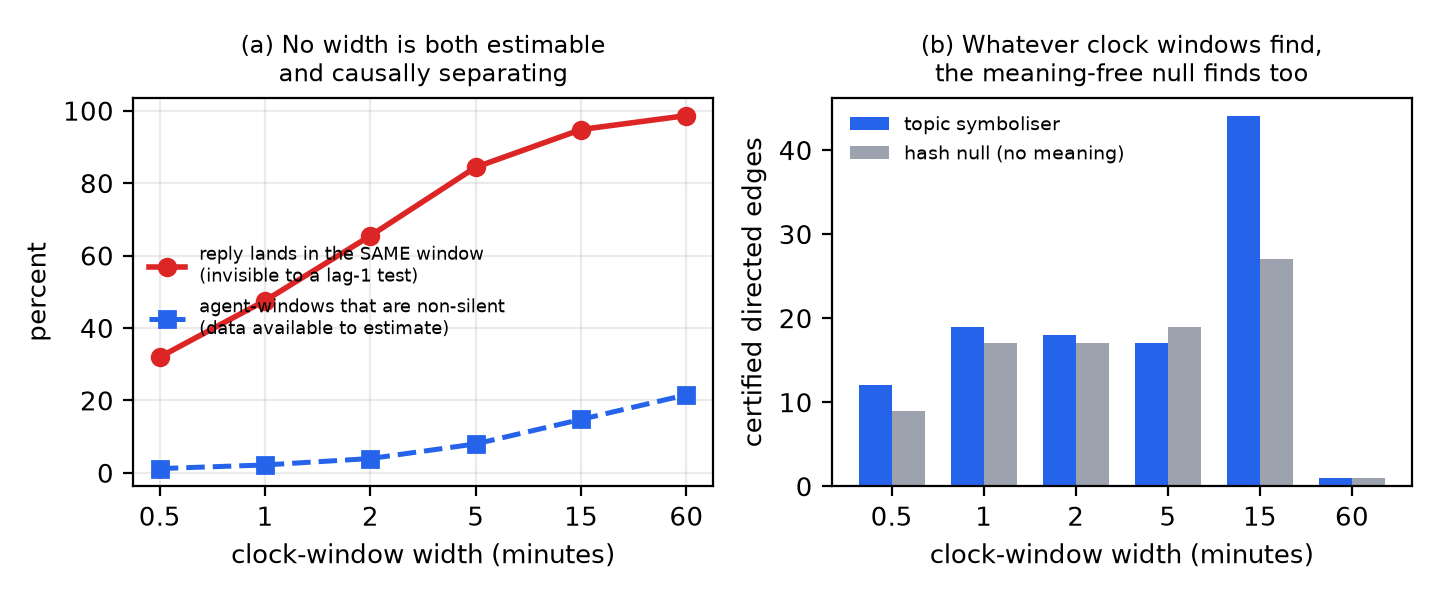
\includegraphics[width=0.92\textwidth]{f1_clock.png}
\caption{Clock-window transfer entropy on the 15 analysed agents of main-village \#general. Left,
the two failure modes as a function of window width. Right, edges certified under the topic
symboliser against the meaning-free hash null.}
\end{figure}

The bind is avoided by ordering messages canonically and letting one message be one tick. Each
agent's series carries its symbol where it spoke and a silent symbol elsewhere, so the lag-1
comparison is between a message and the one immediately before it. The cost is that the measure
captures immediate-predecessor influence only.

\section{The surrogate failure, and two explanations that did not hold}
\label{sec:failure}

An agent is planted into the real stream, drawing its symbols from the channel's marginal and
coupled to nothing at all. It is certified as driving something in 3 of 8 runs when it posts 50
messages, and in 8 of 8 at 100, 263, 600 and 1500 messages, with the mean largest $z$ rising from 5.6
to 12.3, 21.7, 38.3 and 71.7. The error grows with how much the agent speaks, which rules out a
small-sample explanation.

A planted agent could be dismissed as artificial, so the error rate is also measured directly.
Keeping the real speaker sequence and permuting the symbols globally leaves data with no directed
topical influence by construction. The shift surrogate certifies at least one edge in 9 of 10 such
replicates, a family-wise error rate of 0.90 against a nominal 0.05.

\paragraph{What breaks it is the speaker sequence.} Destroying one structure at a time isolates the
cause. Keeping the real speaker order and shuffling only symbols, the shift surrogate fires in 10 of
10 replicates; randomising the speaker order as well drops it to 0 of 10; uniform symbols with the
real order still give 6 of 10. So the driver is the structure of the speaker sequence, not the
symbol distribution and not sparsity. That sequence is far from random in two ways at once: it
repeats a speaker 36\% of the time and returns after one message 38\% of the time, and each agent's
activity is strongly non-stationary, with a median block-share coefficient of variation of 0.79.
Shuffling the order destroys both at once, so this ablation cannot say which of the two mattered.

\subsection{Two explanations I proposed, and the benchmark refuted both}

I initially attributed the failure to mutual exclusivity: only one agent can speak at each tick, so
shifting individual timelines could create overlaps that never occurred in the original
conversation. The benchmark did not support this explanation. A generated channel with exactly one
speaker per tick and steady activity produced an error rate of just 0.025, 95\% Wilson
$[0.011, 0.057]$, far below the 0.90 observed in the real data. Mutual exclusivity alone therefore
cannot explain the failure.

I then suspected turn-taking. In the real channel, speakers repeat 36\% of the time and return after
exactly one message 38\% of the time. However, adding a Markov speaker chain to the generator
produced the opposite result. Turn-taking suppressed the error rather than increasing it. At the
nominal knob values and with no drift the surrogate certified nothing at all across 200 replicates,
while removing turn-taking and introducing drift raised the rate to 0.365. The contribution from
drift was $+0.340$, compared with $-0.025$ for turn-taking. The same inversion appears in the arm
calibrated so that the generated channel reproduces the real channel's measured repeat, return and
block-share statistics rather than merely carrying those numbers as settings: there, turn-taking
alone also certifies nothing, and drift alone gives 0.065.

Neither mechanism, nor their combination in the tested design, reproduced the real-data error rate of
0.90. The largest cell anywhere in the design is 0.365. The real-data ablation removes turn-taking
and non-stationarity together, while the generator separates them. The results point to
non-stationary activity, but the remaining gap means the mechanism behind the full real-data failure
is not yet established.

Every figure above comes from the run at 200 surrogate draws. The first version of this analysis
used 100, which inflates both nulls on the same 2,400 instances: the circular shift fires 53 times
where the 200-draw run does not, against 18 the other way (exact McNemar $p = 3.9 \times 10^{-5}$),
and the permutation surrogate 83 against 20 ($p = 2.7 \times 10^{-10}$). Every qualitative conclusion
in this section is the same at both settings, which is why they are worth stating at all. The
numbers are not, so the draw count belongs in the caption.

\section{The repair, compared}
\label{sec:repair}

Following the local-permutation idea of \citet{runge2018} as adapted by \citet{shorten2021}, each
source keeps its speaking positions and only its symbols are permuted among them. Speaking pattern,
sparsity and turn-taking are preserved exactly, and only the correspondence between symbol and time
is destroyed. On the same destroyed-structure real data the family-wise error rate falls to 0.063
over 300 replicates, 95\% Wilson $[0.041, 0.097]$. The planted uncoupled agent is never certified: 0
of 5 at both 263 and 1500 messages, with mean max $z$ of 2.8 in each case against 22.0 and 68.3
under the shift surrogate.

\begin{figure}[h]
\centering
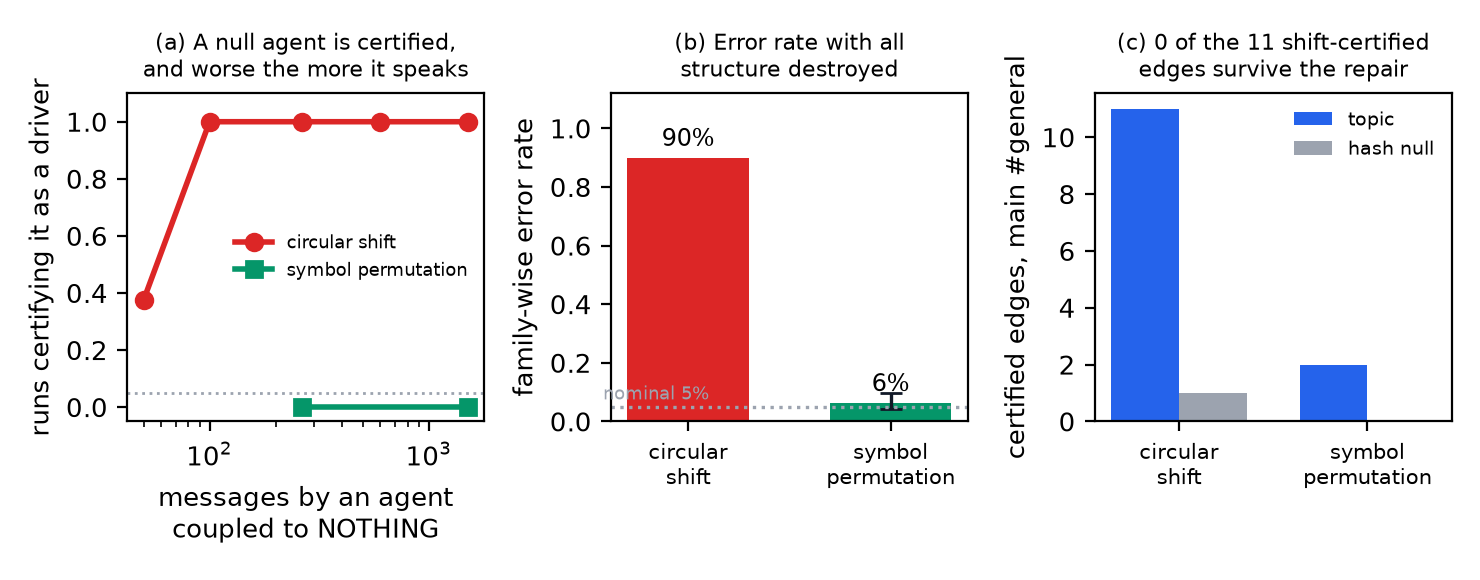
\includegraphics[width=\textwidth]{f2_null.png}
\caption{Left, how often an agent coupled to nothing is certified as a driver, under each surrogate.
Middle, family-wise error rate measured on data with all structure destroyed, with a Wilson
interval; the dotted line is the nominal 0.05. Right, what each surrogate certifies on the real
channel.}
\end{figure}

\subsection{How many surrogate draws are needed}

The number of surrogate draws matters more than I initially appreciated. In a paired comparison of
300 instances, where all four surrogates run on identical symbol grids so the outcomes are paired,
the global permutation surrogate produced a false-positive rate of 0.1167 with 100 draws, falling to
0.0700 with 200 draws, 95\% Wilson $[0.046, 0.105]$. This difference is statistically significant
(exact McNemar $p = 0.0043$). The block-local and Runge local permutations were less sensitive to the
increase: their corresponding rates changed from 0.0900 to 0.0767 and from 0.0967 to 0.0800.

At 200 draws, the global permutation's interval covers the nominal 0.05 and overlaps the real-data
estimate of 0.0633 $[0.0409, 0.0968]$. The real-data result is therefore corroborated rather than
overstated. For practical use, the important point is that reducing the number of surrogate draws
can materially change the result. In particular, the global permutation over-fires at 100 draws by
approximately a factor of two. I would therefore not treat the choice of draw count as a minor
computational detail.

The same correction applies to the benchmark-wide estimate. That figure was 0.0942 at 100 draws.
Repeating all 2,400 instances at 200 draws gives \textbf{0.0679}, 95\% Wilson $[0.0585, 0.0787]$,
and the paired difference is large: 83 instances fire at 100 draws and not at 200, against 20 the
other way, $p = 2.7 \times 10^{-10}$. The conclusion it supports is unchanged, because the interval
still excludes the nominal 0.05. So the permutation repair does carry a residual inflation on clean
generated data, but it is about a third above nominal rather than nearly double.

One limit on this recommendation. I compared 100 draws against 200 and did not test any larger
value, so what the experiment establishes is that 100 is too few, not that 200 is enough. Two
hundred is a lower bound on the draw count rather than a converged setting, and a practitioner whose
conclusions sit near a decision boundary should check their own sensitivity rather than adopt the
number.

\subsection{Choosing a repair, when the error rate cannot choose}

The comparison of the three permutation-based repairs does not produce a clear winner. All four
surrogates were evaluated on identical symbol grids across 300 pure-null replicates, so the
comparison reflects differences between the null models rather than differences between datasets.

\begin{table}[h]
\centering
\begin{tabular}{lrrrl}
\toprule
surrogate & FWER, 100 draws & FWER, 200 draws & 95\% Wilson at 200 & nominal 0.05 \\
\midrule
circular shift                   & 0.0433 & \textbf{0.0333} & $[0.018, 0.060]$ & inside \\
global within-speaker permutation & 0.1167 & \textbf{0.0700} & $[0.046, 0.105]$ & inside \\
block-local permutation          & 0.0900 & \textbf{0.0767} & $[0.052, 0.112]$ & excluded \\
local permutation \citep{runge2018} & 0.0967 & \textbf{0.0800} & $[0.054, 0.116]$ & excluded \\
\bottomrule
\end{tabular}
\caption{Four surrogates on identical symbol grids, 300 pure-null replicates, at both draw counts.}
\end{table}

At 200 draws, paired on the same 300 instances, the circular shift is not significantly different
from the global permutation ($p = 0.0614$), although it differs from block-local permutation
($p = 0.0294$) and from Runge's local permutation ($p = 0.0201$). At 100 draws it differed from all
three, which is the draw-count artifact again. The three repairs remain statistically
indistinguishable from one another, with pairwise $p$-values of 0.85, 0.65 and 1.00. The apparent
differences in their error rates are not sufficient to establish a ranking.

Choosing between them therefore requires more than calibration, and two readings pull against each
other. Runge's local permutation has the strongest methodological justification for preserving the
structure it is intended to preserve, and it follows the approach adapted to event data by
\citet{shorten2021}. Block-local permutation is more heuristic and introduces a free parameter that
has not been tuned. Global permutation is the simplest. On the other hand, the global permutation has
the most favourable interval relative to the nominal rate, and is the only repair that costs nothing
measurable against the shift on clean stationary data, although neither difference is statistically
established. I do not consider the observed error rates sufficient to select one repair over the
others. The choice should be guided by the structure the null is intended to preserve and the
assumptions that can be justified for the data.

\subsection{When to use the repair}

A drift sweep gives the practical reading. Across 150 replicates per cell at 200 surrogate draws,
the circular shift degrades steadily as activity drift increases while the three repairs do not.

\begin{table}[h]
\centering
\begin{tabular}{lrrrr}
\toprule
activity drift & circular shift & global permutation & block-local & local \\
\midrule
0.0 & \textbf{0.013} & 0.093 & 0.080 & 0.093 \\
0.3 & 0.100 & 0.100 & 0.093 & 0.120 \\
0.6 & \textbf{0.193} & 0.053 & 0.047 & 0.067 \\
0.9 & \textbf{0.380} & 0.087 & 0.080 & 0.080 \\
\bottomrule
\end{tabular}
\caption{Family-wise error on pure nulls as activity drift increases, 150 replicates per cell, 200
surrogate draws. Every certified edge is a false positive by construction.}
\end{table}

The pattern is supported by a formal trend test rather than by eye. A Cochran-Armitage test across
the four ordered drift levels gives the circular shift $z = 8.667$, $p < 10^{-15}$, and gives every
repair nothing: $p = 0.51$ for the global permutation, 0.63 for block-local and 0.37 for local. The
same pattern holds at both surrogate draw counts, so it does not depend on that choice.

The repairs are therefore flat under drift rather than calibrated. Only one of the four global
permutation intervals covers the nominal 0.05, and the rest sit nearer 0.09, so what the repair buys
is insensitivity to drift rather than correctness. One asymmetry should be stated rather than
hidden: block-local covers nominal in three of the four cells where the global repair covers one.
The two remain pairwise indistinguishable, so this is not grounds to switch the recommendation, but
it does mean the global repair cannot be described as the best-calibrated under drift.

The results also show why the repair should not be treated as universally preferable. At zero drift
the circular shift has an error rate of 0.013, while the three repairs are all around 0.08 to 0.09.
That advantage is gone by the first drift step: at drift 0.3 the shift reads 0.100 against the global
permutation's 0.100 and block-local's 0.093, so the crossover falls between drift 0.0 and 0.3 rather
than at some higher level. By drift 0.6 the shift is roughly four times the repairs. If a channel has
been checked and found stationary, the circular shift may be sufficient. When activity is
non-stationary the repairs are the more stable choice, and the margin for error on that judgement is
narrow, because the crossover arrives by the first drift level tested.

\section{Continuous time, and what the repair cannot test}

An earlier analysis identified continuous-time estimation as the principled option for event data
but did not evaluate it. Running the continuous-time estimator CoTETE on both channels certifies 0
edges in either case, compared with 2 for main-village and 18 for open-chat under the discrete,
turn-ordered analysis. Its highest $z$-scores are 3.062 and 3.980, below the respective max-T
thresholds of 4.171 and 4.308.

At first these results might appear to contradict the symbol-based analysis. The two estimators
operate on different information, however. CoTETE's public API takes event times with no symbol
channel, while the transfer-entropy analysis here uses topic symbols. To test whether this
difference explains the results, I reduced the data to timing alone, replacing every spoken symbol
with the same code. Under this representation the estimator used here also detects 0 edges in both
channels, matching CoTETE. Using the circular-shift surrogate instead produces 12 and 3 edges. So
neither method detects relationships from event timing alone in these channels, and the edges found
by the symbol-based analysis depend on symbol correspondence, which the continuous-time estimator
cannot access.

Two caveats attach to those $z$-scores, and the second attaches to the larger of them. Point
estimates from this estimator are stochastic to about 17\% across repeated runs, so none of these
values should be read to more than two significant figures. And open-chat's highest $z$, the 3.980,
belongs to the one pair whose surrogate draws mostly failed: it needed 1,936 failed draws to obtain
100 successes, a 4.9\% success rate. Those surrogates are conditioned on being estimable, so that
pair's null is biased in an unknown direction. The conclusion does not rest on it, since that pair
falls below threshold and so does every other pair, but the number should not be quoted as a clean
measurement. The failures themselves were a defect rather than a property of the data: an enlarged
exclusion window can empty the neighbour search on sparse bursty event trains and raise an error
that terminates a whole pair, with no handling at the public entry point. This has been reported
upstream.

There is also a fundamental limitation in applying the recommended permutation surrogate to
timing-only data. When every event carries the same symbol, permuting those symbols changes nothing.
The observed statistic and the surrogate null are identical, making the test exactly degenerate:
standard deviation 0 across all 210 pairs and $p = 1.0$ everywhere. \textbf{The repair has zero power
against timing structure by construction.} The permutation surrogate is appropriate for testing
relationships in the symbol sequence, but it does not answer whether relationships exist in event
timing. These are different questions, and choosing one null means giving up the ability to test the
other with that procedure.

\section{Confounding, and what conditioning removes}

A valid surrogate fixes calibration but not confounding. If every agent tracks a drifting channel
topic, every pair is genuinely dependent through the channel, and pairwise transfer entropy cannot
tell that from direct influence. I therefore also report a \textbf{conditional} estimate, which asks
whether a source's last message adds anything about a target's next one beyond the target's own
history and the channel's recent state. The conditioning variable is the modal symbol of the last
twelve messages, excluding the immediately preceding one so that it does not simply restate the
source.

On a generated benchmark whose decisive instances contain no influence while every agent tracks a
shared drifting topic, so that any certified edge is common cause, pairwise transfer entropy
certifies \textbf{22.3} edges on average and conditioning takes that to \textbf{0.33}, lifting pooled
precision on the four-edge instances from 0.17 to \textbf{0.80} at a recall of 1.0 either way. Across
couplings from 0.05 to 0.8 the conditional test still finds the planted edge in 3 of 3 runs, so the
gain costs no power.

The benchmark flatters the conditional estimator, since its common cause is a shared modal topic and
the conditioning variable is the channel's modal topic. The real channels are harder, and
conditioning there costs degrees of freedom: a 9-symbol alphabet with a 9-valued context gives 6,561
cells against about 7,900 ticks, so that variable is also coarsened to 4 and 2 values.

\begin{table}[h]
\centering
\begin{tabular}{lrrrr}
\toprule
channel & pairwise & conditional, 9 values & 4 values & 2 values \\
\midrule
main \#general      & 2  & \textbf{2, the same two edges} & 2 & 3 \\
open-chat \#general & 18 & \textbf{0} & \textbf{7} & \textbf{13} \\
swarm, room a       & 1  & \textbf{0} & & \\
\bottomrule
\end{tabular}
\caption{Conditioning at three resolutions. Main-village's two edges are robust to that choice;
open-chat's zero is not.}
\end{table}

At the finest resolution the open-chat test is degenerate, its surrogate sitting above the observed
statistic for 65\% of pairs with the largest $z$ in the family only 4.4, so it is failing to reject
rather than finding nothing to reject. Open-chat's structure therefore remains
\textbf{undetermined}: depending on the conditioning resolution, between 0 and 13 of its 18 edges may
survive. That resolution is a free parameter an analyst would set once and never revisit. This is a
property of the channel rather than the estimator: on structure-free real data the conditional test
fires in 2 of 40 replicates, an error rate of 0.05 with a mean $z$ of $-0.001$, so it is nominal
rather than conservative.

\section{The symbolisation floor}
\label{sec:floor}

Everything these methods produce is downstream of turning text into symbols. On the benchmark, where
the underlying topics are known, detection performance drops sharply when agreement between the
symboliser and the ground truth falls below roughly ARI 0.44, and this behaviour appears across the
tested estimators. Importantly, the false-positive rate can look \emph{better} below this point,
because the shared topic structure needed to produce confounded detections is no longer represented
reliably. A pipeline that stops detecting relationships may therefore have lost the signal it needs
rather than become more reliable, and nothing downstream of the symboliser can tell those apart.

\subsection{Detecting the floor without labels}

That degradation can be detected without ground-truth labels. Across the nine-level benchmark sweep,
three statistics separate the below-floor cases with zero errors: seed stability at a threshold of
0.623, agreement with LSA at 0.646, and the Calinski-Harabasz index at 138.9. Seed stability here is
the \textbf{minimum} pairwise agreement across seeds, not the mean; the mean variant makes one error,
at a different threshold of 0.791. Silhouette has the strongest correlation with true ARI, at 0.979,
but is not useful for identifying the boundary because its threshold falls within a gap of just
0.002. A statistic that tracks clustering quality most closely is not necessarily the best one for
making a classification decision.

Error count cannot choose among the three that were perfect, so I tested whether each threshold still
means what it meant when the channel changes for reasons other than topic separability. Applying each
cut unchanged to thirty cells that vary turn-taking, drift, agent count, volume skew, message length
and corpus size, twenty-seven of which hold true ARI at exactly 1.000:

\begin{table}[h]
\centering
\begin{tabular}{lrrrr}
\toprule
diagnostic & cut & errors where fitted & errors, nuisance set & of those at true ARI 1.000 \\
\midrule
seed stability, min across seeds & 0.623 & 0 & 2 & \textbf{0} \\
LSA agreement                    & 0.646 & 0 & 2 & \textbf{0} \\
Calinski-Harabasz                & 138.9 & 0 & 6 & \textbf{3} \\
\bottomrule
\end{tabular}
\caption{Whether a cut fitted on the vocabulary-overlap mechanism survives a change in the channel
that is not a change in topic separability.}
\end{table}

The two bounded statistics err only on the short-message cells, where the symbolisation genuinely has
degraded. Calinski-Harabasz additionally condemns all three cells whose true ARI is exactly 1.000,
for no reason beyond the corpus holding 2,000 messages rather than 8,000, where it reads 76 to 77
against its own cut of 138.9. It is unbounded and grows with sample size, so a published numeric
threshold for it carries no meaning on another corpus. That is why I recommend the two bounded
statistics and not the index that matched them on error count. \textbf{A cut that moves with the
corpus is not a floor cut.}

This is not a weak statistic being discarded on a technicality. Calinski-Harabasz correlates with
true ARI at 0.973, almost as closely as silhouette, and unlike silhouette it classifies the floor
perfectly where it was fitted. It still cannot carry a published threshold. That is the sharper form
of the point above: neither the statistic that tracks quality most closely nor the one that
classifies best on the fitting mechanism is necessarily the one whose cut another researcher can
reuse.

There are important limits to this result. The effective sample size is nine rather than 54, because
the classification label is determined by overlap level. There are no observations between ARI 0.444
and 0.222, so the exact location of the boundary within that interval remains unknown. These
diagnostics classify whether a result is below the tested detection floor; they do not estimate ARI,
and their behaviour is flat between 0.68 and 1.00, and not even monotone there. The benchmark also
uses a single degradation mechanism with a known and correct value of $k$, whereas the true number of
topics in real conversations is unknown. I therefore treat 0.44 as a benchmark-specific, bracketed
result rather than a universal threshold.

\subsection{A contradiction the diagnostic lost}

I initially used these diagnostics to classify one real channel, open-chat, as below the
symbolisation floor. That conclusion did not agree with the channel's measured results: open-chat
certified 18 and 22 edges under the two symbolisers, compared with 2 and 1 for main-village, and its
hash-based null certified zero edges. Rather than treating this disagreement as evidence that the
original measurements were wrong, I revisited the diagnostic itself.

The problem was the choice of $k$. Repeating the comparison with the same channels, loader and window
reproduced the published $k=8$ results to the digit. At $k=4$, however, open-chat reached stability
scores of 0.950 and 0.978, the highest values produced by either channel across the tested settings,
and both exceeded the diagnostic thresholds. The earlier below-floor classification was therefore a
conclusion about one arbitrary choice of $k$, not a reliable statement about the channel. Message
length does not explain the difference either: 27.1\% of main-village messages contain fewer than
five tokens, compared with 2.3\% in open-chat, so the short-message channel is the one the diagnostic
cleared.

This correction changes how the symbolisation results should be read, and it withdrew three claims.

\begin{enumerate}
\item \textbf{The claim that no topic signal remains below the floor is too strong.} The
circular-shift surrogate recovers all four planted edges at every tested overlap level, including
0.95, where ARI is 0.011. The observed collapse is in the permutation null, not necessarily in the
underlying data.
\item \textbf{ARI 0.44 cannot be treated as a universal detection threshold.} When the shared-topic
parameter is 0, detection continues down to ARI 0.296, so the boundary depends on both the
symboliser and the channel.
\item \textbf{Edge counts cannot be used as a measure of symboliser quality.} Even at ARI exactly
1.000, changing the shared-topic parameter alone moves the permutation edge count from 5 to 78.
\end{enumerate}

The diagnostics also do not transfer reliably outside the mechanism on which they were evaluated.
Their balanced accuracy falls from 1.00 to 0.75 and 0.571 under a known mismatch in $k$. All seven
errors made by seed stability are false below-floor classifications, and in every one of those cases
the detector still identifies all planted edges; of the fourteen cells it condemned, eleven had full
conditional recall. The failure direction is the dangerous one: it condemns working symbolisations.

This was an important correction to my own interpretation. I introduced a diagnostic to check whether
the symbolisation was reliable, applied it to the real channels, and found that it contradicted
measurements already in hand. Investigating that contradiction showed the diagnostic was sensitive to
an arbitrary modelling choice. The result is not that the original measurements were wrong, but that
the control was being asked to support a broader conclusion than the evidence allowed. These
diagnostics remain useful within their tested setting, and \textbf{no channel-level floor verdict
should be issued from a single $k$}.

\section{The benchmark}

Real logs have no ground truth, so the common-cause question could not be settled on them. The
generator used here makes the influence graph known by construction: it decides, in code, who speaks
at which tick, on which topic, and who reacts to whom. Surface text is a separate, replaceable layer
drawn from disjoint per-topic vocabularies, so the whole thing runs offline and a detector still has
to symbolise raw text rather than read the labels. Turn-taking and activity drift are independent
knobs, so the two can be varied one at a time, and the generator reproduces its earlier behaviour
bit for bit when both are zero.

\benchname{} is released with 150 tests covering the generator, the detector harness, the text layer,
the floor analysis and the turn-taking factorial.
\ifdeanon{Code and benchmark:
\url{https://github.com/manunicholasjacob/swarm-influence-bench} and
\url{https://github.com/manunicholasjacob/swarm-influence-audit}.}{Code and benchmark are publicly
released; the links are withheld here for anonymity and will be given in the camera-ready version.}

One property of the benchmark must be stated when its numbers are quoted. Planting an edge displaces
other agents' speaking turns, so the generated instances contain real lag-1 dependencies that the
label set does not list. Precision measured against those labels is therefore a \textbf{lower bound}
for any detector, and what the benchmark supports is the comparison between two estimators rather
than the absolute value of either.

\section{What an overseer should do}

Six inexpensive controls should be included whenever an influence graph over an agent channel is
published.

\begin{enumerate}
\item \textbf{Plant an agent coupled to nothing, at your channel's volumes, and check it is not
certified.} This one test would have caught the failure reported here, at one run per volume.
\item \textbf{Measure the error rate directly}, by destroying the structure your method claims to
find and checking the family-wise rate is near nominal. If it is not, your surrogate does not match
your data.
\item \textbf{Preserve the speaker sequence in your surrogate.} Any surrogate that moves an agent's
messages in time will disturb it, and \citet{shorten2021} is the principled route. Use at least 200
surrogate draws, because at 100 the global within-speaker permutation over-fires by roughly a factor
of two.
\item \textbf{Establish the detection floor before interpreting an absence.} ``No edges'' and ``no
influence'' are different claims.
\item \textbf{Condition on the channel, report both numbers, and sweep the resolution.} Pairwise and
conditional bound the answer, and the gap between them is the result. Conditioning costs cells, so
check whether your answer is an artifact of how finely you conditioned. On one channel here it was.
\item \textbf{Report how well your symboliser agrees with the truth, on data where you know it.}
Everything is downstream of turning text into symbols, and below roughly ARI 0.44 detection
collapses whatever the estimator. I have found this control in no influence-detection paper, and it
is also the one that cannot be run on real logs, which is why the floor remains the largest
unquantified threat here.
\end{enumerate}

Two habits follow: publish a meaning-free null's count beside the real one, and require held-out
replication before calling a graph a structure.

\section{The real channels, and what survives}

Re-running every channel under the repaired surrogate changes the answers, and not in one direction.

\begin{table}[h]
\centering
\begin{tabular}{lrrr}
\toprule
channel & window messages & shift: topic / hash & permutation: topic / hash \\
\midrule
main \#general      & 8,800 & 11 / 1 & 2 / 0 \\
open-chat \#general & 8,226 & 3 / 0  & 18 / 0 \\
swarm, room a       & 3,846 & 2 / 1  & 1 / 0 \\
\bottomrule
\end{tabular}
\caption{The same channels under both surrogates, with the meaning-free hash null beside each.}
\end{table}

In main-village, \textbf{none} of the 11 edges the standard recipe certifies survives the repair, and
the two the valid surrogate certifies were not among them. In open-chat the correction runs the other
way, 3 edges becoming 18, because pathological pairs inflate the max-T threshold and raise the bar
for everything else. An invalid surrogate does not simply add false positives; it scrambles the
result.

Main-village's two edges are the strongest thing here and they are still not a finding, because they
do not replicate: the adjacent fourteen-day window certifies nothing at all under either estimator.
Given the detection floor, that silence is as consistent with the test sitting near its limit as with
the edges being absent, and the two cannot be separated. Power is governed by how much an agent says
as much as by how strongly it copies, and it is channel-specific: in main-village a planted follower
copying on 80\% of its messages is caught only 1 time in 4, while in open-chat one copying 10\% of
the time is caught 3 times in 4. Replication is weak everywhere: under the standard recipe the
adjacent window shares 1 edge out of 8 and 4, and that edge is also the only one the hash null
certifies. No certified edge in this work replicates out of sample.

\begin{figure}[h]
\centering
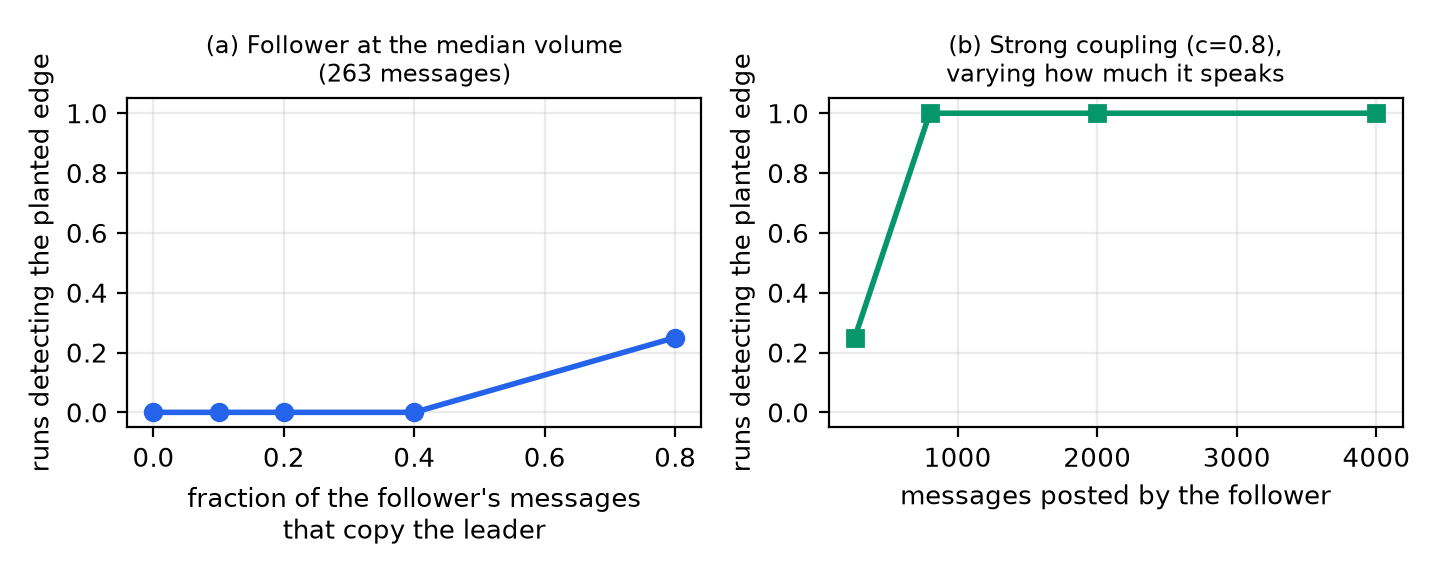
\includegraphics[width=0.92\textwidth]{f4_power.png}
\caption{Detection of a planted follower under the repaired surrogate. Left, varying the fraction of
its messages that copy the leader, at the median agent's volume. Right, varying how much it speaks,
at strong coupling.}
\end{figure}

\paragraph{Humans in the channel.} Main-village \#general is now effectively human-free, with 3 human
messages in the window, so the question has to be asked in open-chat, where 32\% of messages come
from 124 human visitors. Pairwise, with humans collapsed into one node, 19 edges are certified.
Conditioning removes almost all the agent-to-agent structure and little of the rest: \textbf{four
edges survive, of which three run from humans to agents, one is agent to agent, and none run from an
agent to a human.} The asymmetry is not an artifact of the confound. It should be read carefully all
the same: topical dependence from a person to an agent is also what ordinary responsiveness looks
like, so the measurement supports only that the dependence is dyad-specific and directional, not
that anyone is steering a swarm.

\section{Reproducibility, and one limitation of it}

Every number in this paper is recomputed from committed analysis output by a verifier that fails on a
mismatch, and that verifier covers the prose of this paper as well as the figures.

One limitation should be stated plainly. Re-running the counts in the earlier stationarity sweep with
the same seeds and configuration, only one of the eight cells reproduced exactly; the remaining
differences were one or two replicates per cell. Seven of the eight published rates still fell within
the recomputed Wilson intervals, and no conclusion changed. The exception is the zero-drift cell under
the permutation null, where the published 1 of 30 falls just below the recomputed interval of
$[0.035, 0.256]$ for 3 of 30, and no result here depends on that cell.

The generator, estimator and BLAS configuration were investigated and ruled out as the source. The
most likely explanation is a library-level difference, particularly in scikit-learn's $k$-means
implementation within the symboliser, whose output can vary between versions. Every sweep now records
the environment it ran under: Python 3.14.6, numpy 2.5.1, scipy 1.18.0 and scikit-learn 1.9.0,
including the BLAS build and the number of BLAS threads each worker used.

This does not make the previously published counts exactly reproducible. It provides a more clearly
specified environment in which subsequent results can be checked. For that reason I report rates
alongside their confidence intervals rather than exact replicate counts. The distinction between
reproducing a result within its uncertainty and reproducing every individual count matters, and only
the first is claimed.

\section{Conclusion}

Applied to real agent chat, the standard recipe for ``who drives whom'' needs repair before it says
anything. Clock windows cannot separate a message from its answer at the speed agents reply, and what
they certify is matched by a null with no access to meaning. The turn-ordered grid that fixes this
breaks the circular-shift surrogate: family-wise error 0.90 against a nominal 0.05, caused by the
speaker sequence itself. Restricted permutation surrogates repair most of that, but they are flat
under drift rather than calibrated, they are mutually indistinguishable at this precision, and one of
them needs twice the surrogate draws anyone would think to use. A valid surrogate fixes calibration
but not confounding. What survives is small: two dyad-specific edges that do not replicate, an
undetermined answer set by conditioning resolution, and influence running from people into agents and
never back. \textbf{An influence graph should not guide decisions until its error rate, its confound,
its detection floor and its symboliser's fidelity are reported.}

\section*{Limitations}

\begin{itemize}
\item \textbf{Immediate-predecessor only.} The turn-ordered lag-1 measure sees influence from the
message directly before a reply. Influence acting over several turns, or through a room's accumulated
context, is out of scope.
\item \textbf{Discrete approximation to an event process.} Agent chat is event-based in continuous
time. The turn-ordered discretisation with a permutation surrogate is a practical fix, and the
continuous-time comparison above shows what that choice gives up.
\item \textbf{The mechanism behind the real 0.90 is not established.} The generator separates
turn-taking from drift and points at drift, but the largest cell anywhere in the design is 0.365.
\item \textbf{Symbolisation quality cannot be measured on the real logs.} The central result survives
an independent symboliser, but the edge count does not: it moves with alphabet size and with which
messages the topic model is fit on. The floor remains the largest unquantified threat.
\item \textbf{No ground truth in the real logs.} The validity argument rests on planted controls and
on the meaning-free null, not on recovering a known answer.
\item \textbf{Conditioning removes real influence too.} The conditional estimate discards influence
that works by shifting what the channel is talking about, which in a group chat may be a large part
of genuine influence. It is a lower bound on dyadic influence.
\item \textbf{The human result is exploratory.} It rests on one village and one window and should be
read as a lead.
\end{itemize}

\section*{Broader impact and ethics}

This work audits influence detection on a population of AI agents, which is dual-use. Used
defensively it helps an overseer decide what an influence graph is worth, and the main result is
deflationary: it tells practitioners to trust these outputs less, which reduces rather than increases
the chance of acting on a bad attribution. The same tooling could be used to identify the most
influential agent in a swarm in order to target it, or to surveil participants in a channel. Three
properties limit the misuse. The subjects are AI models; the dataset is already public under research
terms and no re-identification is added; and the measure is weak and local, recovering
immediate-predecessor topical dependence rather than any model of how to steer an agent.

The dataset's research terms were followed: research use only, no training on the data, no
re-identification, citation of the source, and notification of the authors of resulting publications.
Human participants appear only as an aggregate node or as anonymised visitor labels, never by name or
handle, and no content attributable to an individual person is reported. Message text and metadata
were read, never model weights or private user data.

The use of a large language model in this work is disclosed in the first-page footnote, as TMLR
requires.

\bibliographystyle{tmlr}
\bibliography{refs}

\end{document}
"               camera-ready
% Use build.py, which runs all of them and checks the anonymous output for leaks.
\providecommand{\TMLRMODE}{submission}
\makeatletter
\def\@tmlrpreprint{preprint}
\def\@tmlraccepted{accepted}
\ifx\TMLRMODE\@tmlrpreprint
  \usepackage[preprint]{tmlr}
\else
  \ifx\TMLRMODE\@tmlraccepted
    \usepackage[accepted]{tmlr}
  \else
    \usepackage{tmlr}
  \fi
\fi
\makeatother

\usepackage{hyperref}
\usepackage{url}
\usepackage{booktabs}
\usepackage{graphicx}
\usepackage{amsmath}

% Gate every identifying string on whether identity may be revealed at all. The flag to test is
% \if@accepted, NOT \if@preprint: tmlr.sty's [preprint] option sets BOTH, so \if@accepted is true
% for the preprint and the camera-ready and false only for the anonymous submission, which is
% exactly the condition wanted. Gating on \if@preprint alone also hid the repository URLs from the
% camera-ready, which is where this paper promises to give them. \if@accepted is internal to
% tmlr.sty, hence the \makeatletter. The anonymous build takes the second argument.
\makeatletter
\newcommand{\ifdeanon}[2]{\if@accepted#1\else#2\fi}
\makeatother
\newcommand{\benchname}{\ifdeanon{SwarmInfluence-Bench}{the benchmark}}

% An unmarked footnote, for the LLM-use disclosure. TMLR's FAQ requires the disclosure and names
% the location: authors must "mention explicitly in their submission that they have used this
% tool", "as a footnote on the first page". Verified against jmlr.org/tmlr/faq.html on 10 Nov 2026.
% It is therefore not optional, and it does not belong in Broader Impact, where it sat until now.
% Nothing in the policy asks for the vendor's name, so none is given.
\newcommand{\disclosurefootnote}[1]{%
  \begingroup\renewcommand\thefootnote{}\footnote{#1}\addtocounter{footnote}{-1}\endgroup}

\title{An Influence Graph Over AI Agents Certifies an Agent That Copies Nobody}

% Hidden by the tmlr package unless [accepted] or [preprint] is given.
\author{\name Manu Nicholas Jacob \email manunicholasjacob@gmail.com \\
        \addr Independent Researcher}

\def\month{11}
\def\year{2026}
\def\openreview{\url{https://openreview.net/forum?id=XXXXXXXXXX}}

\begin{document}
\maketitle

\begin{abstract}
Circular-shift surrogates can produce severely inflated false-positive rates when applied to
turn-ordered multi-agent conversations, reaching a family-wise error rate of 0.90 against a nominal
0.05. A generated benchmark separates two candidate mechanisms and points at non-stationary speaker
activity rather than turn-taking, which suppresses the failure rather than causing it. No setting of
either knob reproduces the observed 0.90, however, so what drives the full real-data failure remains
open. Restricted permutation surrogates substantially reduce the problem. Their error rate is flat
with respect to drift rather than at the nominal level, and for the global within-speaker variant it
depends on how many surrogate draws the null is built from. Calibration alone does not address
confounding, which motivates a conditional estimator validated against a benchmark with planted
ground truth. I also identify a symbolisation-dependent detection limit and develop label-free
diagnostics for it, and show that their calibration does not transport across degradation
mechanisms. The benchmark is released.
\end{abstract}

\disclosurefootnote{\textbf{Use of a large language model.} A large language model was used as an
assistive tool: to help write and run the analysis code, and to help draft this paper. The author is
responsible for every claim, number and figure. All results come from the released code run on the
public dataset, no result or reference is fabricated, and every number in this paper is recomputed
from committed analysis output by a verifier that fails the build on a mismatch.}

\section{Introduction}

When AI agents interact in a shared channel, it is useful to understand how they influence one
another. Information-theoretic methods offer a way to measure this through lagged transfer entropy,
surrogate testing, and per-agent influence scores. They are attractive because they require no
labels and no access to model internals, only a record of who said what and when. The reliability of
those measurements is what this paper examines.

Almost every demonstration of these detectors runs on synthetic traces with a planted leader, where
the analyst controls timing and vocabulary. Real agent chat is asynchronous, bursty, and written in
open language. The narrower question here is whether the standard recipe, applied to real agent
logs, returns anything an overseer should act on.

The audit runs on the AI Village corpus \citep{aidigest2026}, in which frontier models share chat
channels over eighteen months across four villages differing in size, lifetime and tempo, applying
the checks a reader should demand: planted controls, a meaning-free symboliser, replication in a
held-out window, and sensitivity to every parameter that had to be chosen.

\begin{enumerate}
\item The conventional circular-shift surrogate is \textbf{invalid} on turn-ordered agent chat: a
family-wise error rate of 0.90 against a nominal 0.05, caused by the structure of the speaker
sequence itself.
\item Restricted permutation surrogates restore most of the calibration, and re-certifying under one
\textbf{scrambles rather than shrinks} the answer: one channel loses all 11 of its edges, another
gains 15.
\item The three restricted variants are \textbf{mutually indistinguishable} at the precision reached
here, so the choice between them cannot be justified on error rate. The global within-speaker
variant additionally needs on the order of 200 surrogate draws, and over-fires by roughly a factor
of two at 100.
\item Calibration is not confounding, so a conditional estimate is added and validated on a released
benchmark with a known influence graph: common-cause false edges fall from 22.3 to 0.33, and on the
planted-edge instances precision rises from 0.17 to 0.80 with no loss of recall or power.
\item The same benchmark exposes a \textbf{symbolisation floor}. Below roughly 0.44 adjusted Rand
index between symboliser and truth, detection collapses whatever the estimator. Label-free
diagnostics detect that floor, but their calibration does not transport across degradation
mechanisms, and I report where it fails.
\item On the real channels two edges stand at every conditioning resolution, 18 are
\textbf{undetermined} between 0 and 13, none replicates out of sample, and what survives alongside
humans runs from people to agents.
\end{enumerate}

\section{Related work}

\paragraph{Transfer entropy and surrogates.} Transfer entropy \citep{schreiber2000} measures how much
a source's past reduces uncertainty about a target's next symbol beyond the target's own past.
Plug-in estimators are biased upward on short series, so significance rests on surrogate data, with
family-wise error controlled by a max-T test \citep{westfall1993}. The usual surrogate is a circular
time shift of the source.

\paragraph{Event-based data breaks the shift surrogate.} \citet{shorten2021}, on neural spike trains,
show that the conventional source-time-shift surrogate fails to represent the null hypothesis of
conditional independence for event-based processes, and adapt to that setting the nearest-neighbour
local permutation scheme of \citet{runge2018}. Agent chat is event-based in that sense: messages are
events in continuous time, not samples of a clocked signal. The correction is not a contribution of
this paper. The contribution is showing that the same failure carries over to multi-agent safety
monitoring, and that it can be severe enough to create apparent leaders where none exist.

\paragraph{The same failure, concurrently, in multi-agent reinforcement learning.}
\citet{papadopoulos2026} report a closely related surrogate failure in multi-agent
reinforcement-learning action series. Their agent pairs have zero influence by construction, yet
circular time shifts produce false-positive rates of 100\% and 98.2\% against a nominal 0.05. A
plain permutation surrogate fares no better in their setting, at 100.00\% and 99.95\%. Their
proposed correction restricts permutations to blocks of training time, which returns the rates to
5.25\% and 5.50\%.

There are important differences between their setting and this one. Their data consist of binary
actions recorded over twelve thousand training rounds, whereas these data are symbolised
natural-language messages arranged on a turn-ordered conversational grid. Their non-stationarity
comes from monotone drift associated with annealing exploration; here the relevant non-stationarity
appears in the speaker sequence. Neither result should be taken as a direct extension of the other.

Nevertheless, the fact that both approaches rely on restricted permutations is worth noting. Their
permutation blocks are defined by training time, while mine are defined by an agent's own speaking
positions. This provides convergent evidence that unrestricted temporal rearrangement can be
problematic in non-stationary multi-agent data. Their findings also serve as a useful warning for
the approach taken here, and the warning has a measured form rather than a rhetorical one: in their
data the unrestricted permutation failed as completely as the time shift, at 100.00\% against a
nominal 0.05. Permutation-based surrogates are not automatically protected against
non-stationarity, and what protects the one used here is the restriction, not the permutation. I
claim no priority over their result and view the two studies as complementary, addressing different
forms of structured multi-agent data.

\paragraph{Oversight under a budget.} AI-control research frames monitoring as resource constrained,
with a cost for false positives \citep{greenblatt2024}. An influence graph is one such measurement,
and its error rate is the concern here.

\paragraph{Clustering stability.} The idea of using clustering stability as a label-free quality
indicator is not new. It has a substantial history, including \citet{benhur2002},
\citet{lange2004}, von Luxburg's review of clustering stability \citep{vonluxburg2010}, and
\citet{tibshirani2005} on prediction strength. What is different in Section~\ref{sec:floor} is the
calibration of these diagnostics against a detection-performance floor rather than against cluster
recovery alone.

\section{Data and representation}

The AI Village dataset ships one gzipped-JSONL table per village. Four villages are used, differing
enough to test whether any finding is a property of one channel.

\begin{table}[h]
\centering
\begin{tabular}{lrrrrl}
\toprule
village & agent messages & agents & lifetime & human messages & busiest room \\
\midrule
main      & 205,726 & 58  & 576 days & 10,029 & \#general (166,715, 81\%) \\
open-chat &  35,483 & 23  &  66 days & 12,264 & \#general (all) \\
swarm     &   3,848 & 133 &   1 day  &      5 & room a (3,846) \\
game-jam  &     838 & 6   &   3 days &     36 & per-team rooms \\
\bottomrule
\end{tabular}
\caption{The four villages. A 2026 scaffolding change scopes each agent to its current room's
context, so the busiest room of each village is a self-contained influence substrate and is analysed
alone.}
\end{table}

The primary window is the final fourteen days of main-village \#general, 17 to 31 October 2026,
holding 8,800 agent messages. Twenty-two models posted at least 50 messages each and the directed
test uses the 15 busiest, giving 7,958 message events. Two scaffolding facts are disclosed rather
than corrected: the automated nudger was off throughout, and the unused \#best and \#rest rooms were
soft-deleted mid-window, which does not touch \#general.

\subsection{From open language to symbols}

Transfer entropy needs discrete symbols, so each message is mapped to a small alphabet before
influence is estimated, and that mapping is kept separate from the estimator. A topic symboliser
(TF-IDF then $k$-means, $k=8$) gives a message its topic cluster id, so paraphrases of one idea share
a symbol. A hash symboliser, a stable hash of the normalised text into $k=8$ buckets, has no notion
of meaning and serves as a null: an edge appearing under both lives in timing alone.

\subsection{The lag problem, and why clock windows cannot solve it}

A lag-1 transfer entropy compares window $t-1$ with window $t$, so influence landing inside one
window is invisible to it. Agent chat makes this binding. Among the fifteen analysed agents the gap
between consecutive messages by different speakers has a median of 28.1 seconds (25th percentile
9.2, 75th 66.2, 95th 159.3), so turn-taking is a seconds-scale process while any clock window wide
enough to hold two speakers is minutes wide and swallows both a message and its answer.

Both horns are measurable. At 30 seconds only 1.2\% of agent-windows hold a message, while 32.0\% of
replies already land in the same window as what they answer, rising to 84.4\% at five minutes. At
every width tried, the meaning-free hash null certifies comparably many edges, and more at five
minutes: 9 against 12 at thirty seconds, 17 against 19 at one minute, 27 against 44 at fifteen, and
19 against 17 at five. Whatever clock-window transfer entropy was detecting there, it was not shared
meaning.

\begin{figure}[h]
\centering
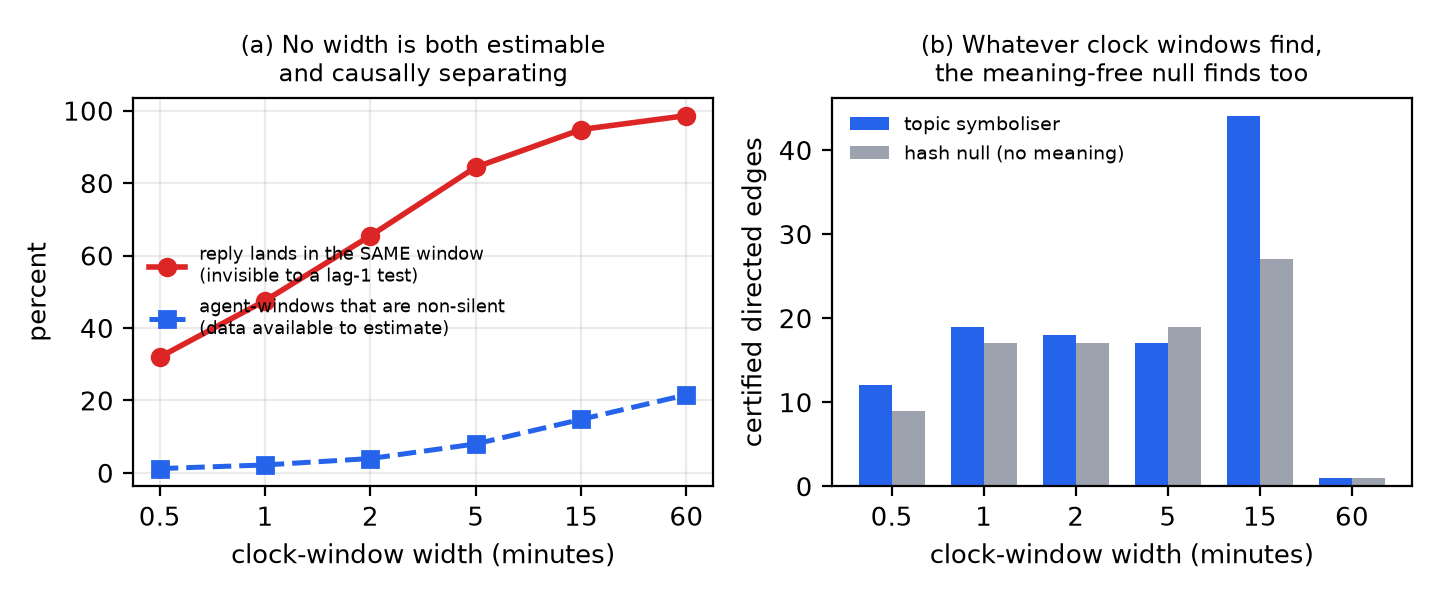
\includegraphics[width=0.92\textwidth]{f1_clock.png}
\caption{Clock-window transfer entropy on the 15 analysed agents of main-village \#general. Left,
the two failure modes as a function of window width. Right, edges certified under the topic
symboliser against the meaning-free hash null.}
\end{figure}

The bind is avoided by ordering messages canonically and letting one message be one tick. Each
agent's series carries its symbol where it spoke and a silent symbol elsewhere, so the lag-1
comparison is between a message and the one immediately before it. The cost is that the measure
captures immediate-predecessor influence only.

\section{The surrogate failure, and two explanations that did not hold}
\label{sec:failure}

An agent is planted into the real stream, drawing its symbols from the channel's marginal and
coupled to nothing at all. It is certified as driving something in 3 of 8 runs when it posts 50
messages, and in 8 of 8 at 100, 263, 600 and 1500 messages, with the mean largest $z$ rising from 5.6
to 12.3, 21.7, 38.3 and 71.7. The error grows with how much the agent speaks, which rules out a
small-sample explanation.

A planted agent could be dismissed as artificial, so the error rate is also measured directly.
Keeping the real speaker sequence and permuting the symbols globally leaves data with no directed
topical influence by construction. The shift surrogate certifies at least one edge in 9 of 10 such
replicates, a family-wise error rate of 0.90 against a nominal 0.05.

\paragraph{What breaks it is the speaker sequence.} Destroying one structure at a time isolates the
cause. Keeping the real speaker order and shuffling only symbols, the shift surrogate fires in 10 of
10 replicates; randomising the speaker order as well drops it to 0 of 10; uniform symbols with the
real order still give 6 of 10. So the driver is the structure of the speaker sequence, not the
symbol distribution and not sparsity. That sequence is far from random in two ways at once: it
repeats a speaker 36\% of the time and returns after one message 38\% of the time, and each agent's
activity is strongly non-stationary, with a median block-share coefficient of variation of 0.79.
Shuffling the order destroys both at once, so this ablation cannot say which of the two mattered.

\subsection{Two explanations I proposed, and the benchmark refuted both}

I initially attributed the failure to mutual exclusivity: only one agent can speak at each tick, so
shifting individual timelines could create overlaps that never occurred in the original
conversation. The benchmark did not support this explanation. A generated channel with exactly one
speaker per tick and steady activity produced an error rate of just 0.025, 95\% Wilson
$[0.011, 0.057]$, far below the 0.90 observed in the real data. Mutual exclusivity alone therefore
cannot explain the failure.

I then suspected turn-taking. In the real channel, speakers repeat 36\% of the time and return after
exactly one message 38\% of the time. However, adding a Markov speaker chain to the generator
produced the opposite result. Turn-taking suppressed the error rather than increasing it. At the
nominal knob values and with no drift the surrogate certified nothing at all across 200 replicates,
while removing turn-taking and introducing drift raised the rate to 0.365. The contribution from
drift was $+0.340$, compared with $-0.025$ for turn-taking. The same inversion appears in the arm
calibrated so that the generated channel reproduces the real channel's measured repeat, return and
block-share statistics rather than merely carrying those numbers as settings: there, turn-taking
alone also certifies nothing, and drift alone gives 0.065.

Neither mechanism, nor their combination in the tested design, reproduced the real-data error rate of
0.90. The largest cell anywhere in the design is 0.365. The real-data ablation removes turn-taking
and non-stationarity together, while the generator separates them. The results point to
non-stationary activity, but the remaining gap means the mechanism behind the full real-data failure
is not yet established.

Every figure above comes from the run at 200 surrogate draws. The first version of this analysis
used 100, which inflates both nulls on the same 2,400 instances: the circular shift fires 53 times
where the 200-draw run does not, against 18 the other way (exact McNemar $p = 3.9 \times 10^{-5}$),
and the permutation surrogate 83 against 20 ($p = 2.7 \times 10^{-10}$). Every qualitative conclusion
in this section is the same at both settings, which is why they are worth stating at all. The
numbers are not, so the draw count belongs in the caption.

\section{The repair, compared}
\label{sec:repair}

Following the local-permutation idea of \citet{runge2018} as adapted by \citet{shorten2021}, each
source keeps its speaking positions and only its symbols are permuted among them. Speaking pattern,
sparsity and turn-taking are preserved exactly, and only the correspondence between symbol and time
is destroyed. On the same destroyed-structure real data the family-wise error rate falls to 0.063
over 300 replicates, 95\% Wilson $[0.041, 0.097]$. The planted uncoupled agent is never certified: 0
of 5 at both 263 and 1500 messages, with mean max $z$ of 2.8 in each case against 22.0 and 68.3
under the shift surrogate.

\begin{figure}[h]
\centering
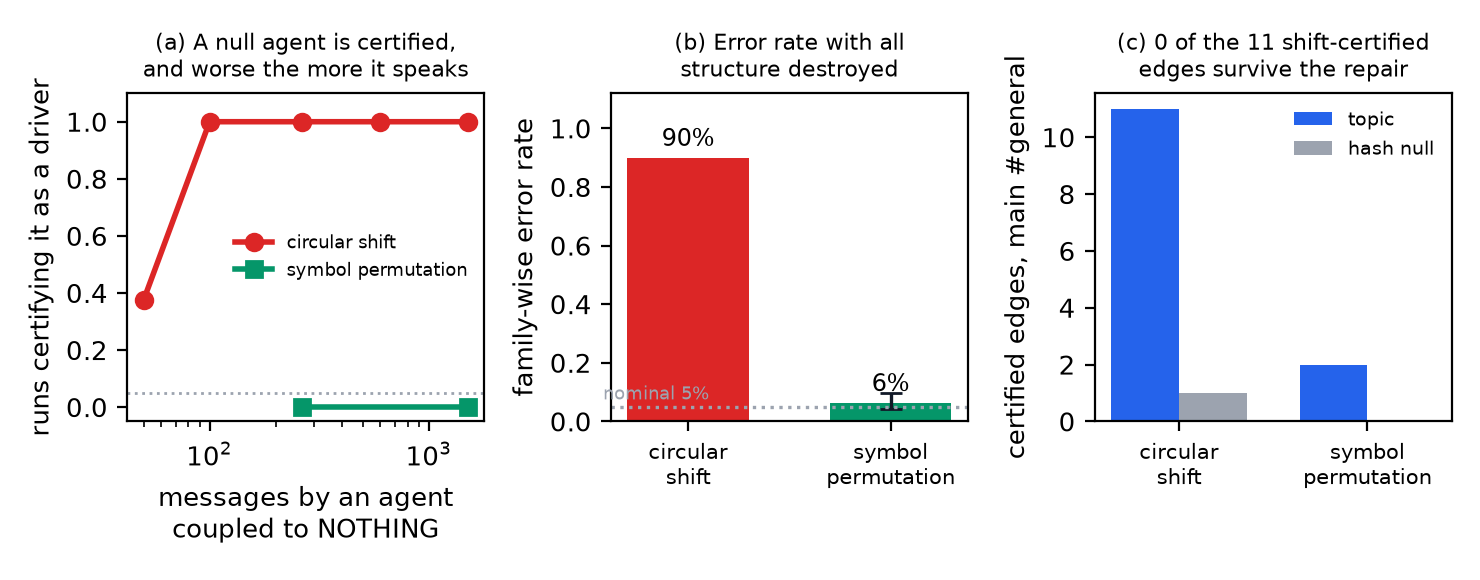
\includegraphics[width=\textwidth]{f2_null.png}
\caption{Left, how often an agent coupled to nothing is certified as a driver, under each surrogate.
Middle, family-wise error rate measured on data with all structure destroyed, with a Wilson
interval; the dotted line is the nominal 0.05. Right, what each surrogate certifies on the real
channel.}
\end{figure}

\subsection{How many surrogate draws are needed}

The number of surrogate draws matters more than I initially appreciated. In a paired comparison of
300 instances, where all four surrogates run on identical symbol grids so the outcomes are paired,
the global permutation surrogate produced a false-positive rate of 0.1167 with 100 draws, falling to
0.0700 with 200 draws, 95\% Wilson $[0.046, 0.105]$. This difference is statistically significant
(exact McNemar $p = 0.0043$). The block-local and Runge local permutations were less sensitive to the
increase: their corresponding rates changed from 0.0900 to 0.0767 and from 0.0967 to 0.0800.

At 200 draws, the global permutation's interval covers the nominal 0.05 and overlaps the real-data
estimate of 0.0633 $[0.0409, 0.0968]$. The real-data result is therefore corroborated rather than
overstated. For practical use, the important point is that reducing the number of surrogate draws
can materially change the result. In particular, the global permutation over-fires at 100 draws by
approximately a factor of two. I would therefore not treat the choice of draw count as a minor
computational detail.

The same correction applies to the benchmark-wide estimate. That figure was 0.0942 at 100 draws.
Repeating all 2,400 instances at 200 draws gives \textbf{0.0679}, 95\% Wilson $[0.0585, 0.0787]$,
and the paired difference is large: 83 instances fire at 100 draws and not at 200, against 20 the
other way, $p = 2.7 \times 10^{-10}$. The conclusion it supports is unchanged, because the interval
still excludes the nominal 0.05. So the permutation repair does carry a residual inflation on clean
generated data, but it is about a third above nominal rather than nearly double.

One limit on this recommendation. I compared 100 draws against 200 and did not test any larger
value, so what the experiment establishes is that 100 is too few, not that 200 is enough. Two
hundred is a lower bound on the draw count rather than a converged setting, and a practitioner whose
conclusions sit near a decision boundary should check their own sensitivity rather than adopt the
number.

\subsection{Choosing a repair, when the error rate cannot choose}

The comparison of the three permutation-based repairs does not produce a clear winner. All four
surrogates were evaluated on identical symbol grids across 300 pure-null replicates, so the
comparison reflects differences between the null models rather than differences between datasets.

\begin{table}[h]
\centering
\begin{tabular}{lrrrl}
\toprule
surrogate & FWER, 100 draws & FWER, 200 draws & 95\% Wilson at 200 & nominal 0.05 \\
\midrule
circular shift                   & 0.0433 & \textbf{0.0333} & $[0.018, 0.060]$ & inside \\
global within-speaker permutation & 0.1167 & \textbf{0.0700} & $[0.046, 0.105]$ & inside \\
block-local permutation          & 0.0900 & \textbf{0.0767} & $[0.052, 0.112]$ & excluded \\
local permutation \citep{runge2018} & 0.0967 & \textbf{0.0800} & $[0.054, 0.116]$ & excluded \\
\bottomrule
\end{tabular}
\caption{Four surrogates on identical symbol grids, 300 pure-null replicates, at both draw counts.}
\end{table}

At 200 draws, paired on the same 300 instances, the circular shift is not significantly different
from the global permutation ($p = 0.0614$), although it differs from block-local permutation
($p = 0.0294$) and from Runge's local permutation ($p = 0.0201$). At 100 draws it differed from all
three, which is the draw-count artifact again. The three repairs remain statistically
indistinguishable from one another, with pairwise $p$-values of 0.85, 0.65 and 1.00. The apparent
differences in their error rates are not sufficient to establish a ranking.

Choosing between them therefore requires more than calibration, and two readings pull against each
other. Runge's local permutation has the strongest methodological justification for preserving the
structure it is intended to preserve, and it follows the approach adapted to event data by
\citet{shorten2021}. Block-local permutation is more heuristic and introduces a free parameter that
has not been tuned. Global permutation is the simplest. On the other hand, the global permutation has
the most favourable interval relative to the nominal rate, and is the only repair that costs nothing
measurable against the shift on clean stationary data, although neither difference is statistically
established. I do not consider the observed error rates sufficient to select one repair over the
others. The choice should be guided by the structure the null is intended to preserve and the
assumptions that can be justified for the data.

\subsection{When to use the repair}

A drift sweep gives the practical reading. Across 150 replicates per cell at 200 surrogate draws,
the circular shift degrades steadily as activity drift increases while the three repairs do not.

\begin{table}[h]
\centering
\begin{tabular}{lrrrr}
\toprule
activity drift & circular shift & global permutation & block-local & local \\
\midrule
0.0 & \textbf{0.013} & 0.093 & 0.080 & 0.093 \\
0.3 & 0.100 & 0.100 & 0.093 & 0.120 \\
0.6 & \textbf{0.193} & 0.053 & 0.047 & 0.067 \\
0.9 & \textbf{0.380} & 0.087 & 0.080 & 0.080 \\
\bottomrule
\end{tabular}
\caption{Family-wise error on pure nulls as activity drift increases, 150 replicates per cell, 200
surrogate draws. Every certified edge is a false positive by construction.}
\end{table}

The pattern is supported by a formal trend test rather than by eye. A Cochran-Armitage test across
the four ordered drift levels gives the circular shift $z = 8.667$, $p < 10^{-15}$, and gives every
repair nothing: $p = 0.51$ for the global permutation, 0.63 for block-local and 0.37 for local. The
same pattern holds at both surrogate draw counts, so it does not depend on that choice.

The repairs are therefore flat under drift rather than calibrated. Only one of the four global
permutation intervals covers the nominal 0.05, and the rest sit nearer 0.09, so what the repair buys
is insensitivity to drift rather than correctness. One asymmetry should be stated rather than
hidden: block-local covers nominal in three of the four cells where the global repair covers one.
The two remain pairwise indistinguishable, so this is not grounds to switch the recommendation, but
it does mean the global repair cannot be described as the best-calibrated under drift.

The results also show why the repair should not be treated as universally preferable. At zero drift
the circular shift has an error rate of 0.013, while the three repairs are all around 0.08 to 0.09.
That advantage is gone by the first drift step: at drift 0.3 the shift reads 0.100 against the global
permutation's 0.100 and block-local's 0.093, so the crossover falls between drift 0.0 and 0.3 rather
than at some higher level. By drift 0.6 the shift is roughly four times the repairs. If a channel has
been checked and found stationary, the circular shift may be sufficient. When activity is
non-stationary the repairs are the more stable choice, and the margin for error on that judgement is
narrow, because the crossover arrives by the first drift level tested.

\section{Continuous time, and what the repair cannot test}

An earlier analysis identified continuous-time estimation as the principled option for event data
but did not evaluate it. Running the continuous-time estimator CoTETE on both channels certifies 0
edges in either case, compared with 2 for main-village and 18 for open-chat under the discrete,
turn-ordered analysis. Its highest $z$-scores are 3.062 and 3.980, below the respective max-T
thresholds of 4.171 and 4.308.

At first these results might appear to contradict the symbol-based analysis. The two estimators
operate on different information, however. CoTETE's public API takes event times with no symbol
channel, while the transfer-entropy analysis here uses topic symbols. To test whether this
difference explains the results, I reduced the data to timing alone, replacing every spoken symbol
with the same code. Under this representation the estimator used here also detects 0 edges in both
channels, matching CoTETE. Using the circular-shift surrogate instead produces 12 and 3 edges. So
neither method detects relationships from event timing alone in these channels, and the edges found
by the symbol-based analysis depend on symbol correspondence, which the continuous-time estimator
cannot access.

Two caveats attach to those $z$-scores, and the second attaches to the larger of them. Point
estimates from this estimator are stochastic to about 17\% across repeated runs, so none of these
values should be read to more than two significant figures. And open-chat's highest $z$, the 3.980,
belongs to the one pair whose surrogate draws mostly failed: it needed 1,936 failed draws to obtain
100 successes, a 4.9\% success rate. Those surrogates are conditioned on being estimable, so that
pair's null is biased in an unknown direction. The conclusion does not rest on it, since that pair
falls below threshold and so does every other pair, but the number should not be quoted as a clean
measurement. The failures themselves were a defect rather than a property of the data: an enlarged
exclusion window can empty the neighbour search on sparse bursty event trains and raise an error
that terminates a whole pair, with no handling at the public entry point. This has been reported
upstream.

There is also a fundamental limitation in applying the recommended permutation surrogate to
timing-only data. When every event carries the same symbol, permuting those symbols changes nothing.
The observed statistic and the surrogate null are identical, making the test exactly degenerate:
standard deviation 0 across all 210 pairs and $p = 1.0$ everywhere. \textbf{The repair has zero power
against timing structure by construction.} The permutation surrogate is appropriate for testing
relationships in the symbol sequence, but it does not answer whether relationships exist in event
timing. These are different questions, and choosing one null means giving up the ability to test the
other with that procedure.

\section{Confounding, and what conditioning removes}

A valid surrogate fixes calibration but not confounding. If every agent tracks a drifting channel
topic, every pair is genuinely dependent through the channel, and pairwise transfer entropy cannot
tell that from direct influence. I therefore also report a \textbf{conditional} estimate, which asks
whether a source's last message adds anything about a target's next one beyond the target's own
history and the channel's recent state. The conditioning variable is the modal symbol of the last
twelve messages, excluding the immediately preceding one so that it does not simply restate the
source.

On a generated benchmark whose decisive instances contain no influence while every agent tracks a
shared drifting topic, so that any certified edge is common cause, pairwise transfer entropy
certifies \textbf{22.3} edges on average and conditioning takes that to \textbf{0.33}, lifting pooled
precision on the four-edge instances from 0.17 to \textbf{0.80} at a recall of 1.0 either way. Across
couplings from 0.05 to 0.8 the conditional test still finds the planted edge in 3 of 3 runs, so the
gain costs no power.

The benchmark flatters the conditional estimator, since its common cause is a shared modal topic and
the conditioning variable is the channel's modal topic. The real channels are harder, and
conditioning there costs degrees of freedom: a 9-symbol alphabet with a 9-valued context gives 6,561
cells against about 7,900 ticks, so that variable is also coarsened to 4 and 2 values.

\begin{table}[h]
\centering
\begin{tabular}{lrrrr}
\toprule
channel & pairwise & conditional, 9 values & 4 values & 2 values \\
\midrule
main \#general      & 2  & \textbf{2, the same two edges} & 2 & 3 \\
open-chat \#general & 18 & \textbf{0} & \textbf{7} & \textbf{13} \\
swarm, room a       & 1  & \textbf{0} & & \\
\bottomrule
\end{tabular}
\caption{Conditioning at three resolutions. Main-village's two edges are robust to that choice;
open-chat's zero is not.}
\end{table}

At the finest resolution the open-chat test is degenerate, its surrogate sitting above the observed
statistic for 65\% of pairs with the largest $z$ in the family only 4.4, so it is failing to reject
rather than finding nothing to reject. Open-chat's structure therefore remains
\textbf{undetermined}: depending on the conditioning resolution, between 0 and 13 of its 18 edges may
survive. That resolution is a free parameter an analyst would set once and never revisit. This is a
property of the channel rather than the estimator: on structure-free real data the conditional test
fires in 2 of 40 replicates, an error rate of 0.05 with a mean $z$ of $-0.001$, so it is nominal
rather than conservative.

\section{The symbolisation floor}
\label{sec:floor}

Everything these methods produce is downstream of turning text into symbols. On the benchmark, where
the underlying topics are known, detection performance drops sharply when agreement between the
symboliser and the ground truth falls below roughly ARI 0.44, and this behaviour appears across the
tested estimators. Importantly, the false-positive rate can look \emph{better} below this point,
because the shared topic structure needed to produce confounded detections is no longer represented
reliably. A pipeline that stops detecting relationships may therefore have lost the signal it needs
rather than become more reliable, and nothing downstream of the symboliser can tell those apart.

\subsection{Detecting the floor without labels}

That degradation can be detected without ground-truth labels. Across the nine-level benchmark sweep,
three statistics separate the below-floor cases with zero errors: seed stability at a threshold of
0.623, agreement with LSA at 0.646, and the Calinski-Harabasz index at 138.9. Seed stability here is
the \textbf{minimum} pairwise agreement across seeds, not the mean; the mean variant makes one error,
at a different threshold of 0.791. Silhouette has the strongest correlation with true ARI, at 0.979,
but is not useful for identifying the boundary because its threshold falls within a gap of just
0.002. A statistic that tracks clustering quality most closely is not necessarily the best one for
making a classification decision.

Error count cannot choose among the three that were perfect, so I tested whether each threshold still
means what it meant when the channel changes for reasons other than topic separability. Applying each
cut unchanged to thirty cells that vary turn-taking, drift, agent count, volume skew, message length
and corpus size, twenty-seven of which hold true ARI at exactly 1.000:

\begin{table}[h]
\centering
\begin{tabular}{lrrrr}
\toprule
diagnostic & cut & errors where fitted & errors, nuisance set & of those at true ARI 1.000 \\
\midrule
seed stability, min across seeds & 0.623 & 0 & 2 & \textbf{0} \\
LSA agreement                    & 0.646 & 0 & 2 & \textbf{0} \\
Calinski-Harabasz                & 138.9 & 0 & 6 & \textbf{3} \\
\bottomrule
\end{tabular}
\caption{Whether a cut fitted on the vocabulary-overlap mechanism survives a change in the channel
that is not a change in topic separability.}
\end{table}

The two bounded statistics err only on the short-message cells, where the symbolisation genuinely has
degraded. Calinski-Harabasz additionally condemns all three cells whose true ARI is exactly 1.000,
for no reason beyond the corpus holding 2,000 messages rather than 8,000, where it reads 76 to 77
against its own cut of 138.9. It is unbounded and grows with sample size, so a published numeric
threshold for it carries no meaning on another corpus. That is why I recommend the two bounded
statistics and not the index that matched them on error count. \textbf{A cut that moves with the
corpus is not a floor cut.}

This is not a weak statistic being discarded on a technicality. Calinski-Harabasz correlates with
true ARI at 0.973, almost as closely as silhouette, and unlike silhouette it classifies the floor
perfectly where it was fitted. It still cannot carry a published threshold. That is the sharper form
of the point above: neither the statistic that tracks quality most closely nor the one that
classifies best on the fitting mechanism is necessarily the one whose cut another researcher can
reuse.

There are important limits to this result. The effective sample size is nine rather than 54, because
the classification label is determined by overlap level. There are no observations between ARI 0.444
and 0.222, so the exact location of the boundary within that interval remains unknown. These
diagnostics classify whether a result is below the tested detection floor; they do not estimate ARI,
and their behaviour is flat between 0.68 and 1.00, and not even monotone there. The benchmark also
uses a single degradation mechanism with a known and correct value of $k$, whereas the true number of
topics in real conversations is unknown. I therefore treat 0.44 as a benchmark-specific, bracketed
result rather than a universal threshold.

\subsection{A contradiction the diagnostic lost}

I initially used these diagnostics to classify one real channel, open-chat, as below the
symbolisation floor. That conclusion did not agree with the channel's measured results: open-chat
certified 18 and 22 edges under the two symbolisers, compared with 2 and 1 for main-village, and its
hash-based null certified zero edges. Rather than treating this disagreement as evidence that the
original measurements were wrong, I revisited the diagnostic itself.

The problem was the choice of $k$. Repeating the comparison with the same channels, loader and window
reproduced the published $k=8$ results to the digit. At $k=4$, however, open-chat reached stability
scores of 0.950 and 0.978, the highest values produced by either channel across the tested settings,
and both exceeded the diagnostic thresholds. The earlier below-floor classification was therefore a
conclusion about one arbitrary choice of $k$, not a reliable statement about the channel. Message
length does not explain the difference either: 27.1\% of main-village messages contain fewer than
five tokens, compared with 2.3\% in open-chat, so the short-message channel is the one the diagnostic
cleared.

This correction changes how the symbolisation results should be read, and it withdrew three claims.

\begin{enumerate}
\item \textbf{The claim that no topic signal remains below the floor is too strong.} The
circular-shift surrogate recovers all four planted edges at every tested overlap level, including
0.95, where ARI is 0.011. The observed collapse is in the permutation null, not necessarily in the
underlying data.
\item \textbf{ARI 0.44 cannot be treated as a universal detection threshold.} When the shared-topic
parameter is 0, detection continues down to ARI 0.296, so the boundary depends on both the
symboliser and the channel.
\item \textbf{Edge counts cannot be used as a measure of symboliser quality.} Even at ARI exactly
1.000, changing the shared-topic parameter alone moves the permutation edge count from 5 to 78.
\end{enumerate}

The diagnostics also do not transfer reliably outside the mechanism on which they were evaluated.
Their balanced accuracy falls from 1.00 to 0.75 and 0.571 under a known mismatch in $k$. All seven
errors made by seed stability are false below-floor classifications, and in every one of those cases
the detector still identifies all planted edges; of the fourteen cells it condemned, eleven had full
conditional recall. The failure direction is the dangerous one: it condemns working symbolisations.

This was an important correction to my own interpretation. I introduced a diagnostic to check whether
the symbolisation was reliable, applied it to the real channels, and found that it contradicted
measurements already in hand. Investigating that contradiction showed the diagnostic was sensitive to
an arbitrary modelling choice. The result is not that the original measurements were wrong, but that
the control was being asked to support a broader conclusion than the evidence allowed. These
diagnostics remain useful within their tested setting, and \textbf{no channel-level floor verdict
should be issued from a single $k$}.

\section{The benchmark}

Real logs have no ground truth, so the common-cause question could not be settled on them. The
generator used here makes the influence graph known by construction: it decides, in code, who speaks
at which tick, on which topic, and who reacts to whom. Surface text is a separate, replaceable layer
drawn from disjoint per-topic vocabularies, so the whole thing runs offline and a detector still has
to symbolise raw text rather than read the labels. Turn-taking and activity drift are independent
knobs, so the two can be varied one at a time, and the generator reproduces its earlier behaviour
bit for bit when both are zero.

\benchname{} is released with 150 tests covering the generator, the detector harness, the text layer,
the floor analysis and the turn-taking factorial.
\ifdeanon{Code and benchmark:
\url{https://github.com/manunicholasjacob/swarm-influence-bench} and
\url{https://github.com/manunicholasjacob/swarm-influence-audit}.}{Code and benchmark are publicly
released; the links are withheld here for anonymity and will be given in the camera-ready version.}

One property of the benchmark must be stated when its numbers are quoted. Planting an edge displaces
other agents' speaking turns, so the generated instances contain real lag-1 dependencies that the
label set does not list. Precision measured against those labels is therefore a \textbf{lower bound}
for any detector, and what the benchmark supports is the comparison between two estimators rather
than the absolute value of either.

\section{What an overseer should do}

Six inexpensive controls should be included whenever an influence graph over an agent channel is
published.

\begin{enumerate}
\item \textbf{Plant an agent coupled to nothing, at your channel's volumes, and check it is not
certified.} This one test would have caught the failure reported here, at one run per volume.
\item \textbf{Measure the error rate directly}, by destroying the structure your method claims to
find and checking the family-wise rate is near nominal. If it is not, your surrogate does not match
your data.
\item \textbf{Preserve the speaker sequence in your surrogate.} Any surrogate that moves an agent's
messages in time will disturb it, and \citet{shorten2021} is the principled route. Use at least 200
surrogate draws, because at 100 the global within-speaker permutation over-fires by roughly a factor
of two.
\item \textbf{Establish the detection floor before interpreting an absence.} ``No edges'' and ``no
influence'' are different claims.
\item \textbf{Condition on the channel, report both numbers, and sweep the resolution.} Pairwise and
conditional bound the answer, and the gap between them is the result. Conditioning costs cells, so
check whether your answer is an artifact of how finely you conditioned. On one channel here it was.
\item \textbf{Report how well your symboliser agrees with the truth, on data where you know it.}
Everything is downstream of turning text into symbols, and below roughly ARI 0.44 detection
collapses whatever the estimator. I have found this control in no influence-detection paper, and it
is also the one that cannot be run on real logs, which is why the floor remains the largest
unquantified threat here.
\end{enumerate}

Two habits follow: publish a meaning-free null's count beside the real one, and require held-out
replication before calling a graph a structure.

\section{The real channels, and what survives}

Re-running every channel under the repaired surrogate changes the answers, and not in one direction.

\begin{table}[h]
\centering
\begin{tabular}{lrrr}
\toprule
channel & window messages & shift: topic / hash & permutation: topic / hash \\
\midrule
main \#general      & 8,800 & 11 / 1 & 2 / 0 \\
open-chat \#general & 8,226 & 3 / 0  & 18 / 0 \\
swarm, room a       & 3,846 & 2 / 1  & 1 / 0 \\
\bottomrule
\end{tabular}
\caption{The same channels under both surrogates, with the meaning-free hash null beside each.}
\end{table}

In main-village, \textbf{none} of the 11 edges the standard recipe certifies survives the repair, and
the two the valid surrogate certifies were not among them. In open-chat the correction runs the other
way, 3 edges becoming 18, because pathological pairs inflate the max-T threshold and raise the bar
for everything else. An invalid surrogate does not simply add false positives; it scrambles the
result.

Main-village's two edges are the strongest thing here and they are still not a finding, because they
do not replicate: the adjacent fourteen-day window certifies nothing at all under either estimator.
Given the detection floor, that silence is as consistent with the test sitting near its limit as with
the edges being absent, and the two cannot be separated. Power is governed by how much an agent says
as much as by how strongly it copies, and it is channel-specific: in main-village a planted follower
copying on 80\% of its messages is caught only 1 time in 4, while in open-chat one copying 10\% of
the time is caught 3 times in 4. Replication is weak everywhere: under the standard recipe the
adjacent window shares 1 edge out of 8 and 4, and that edge is also the only one the hash null
certifies. No certified edge in this work replicates out of sample.

\begin{figure}[h]
\centering
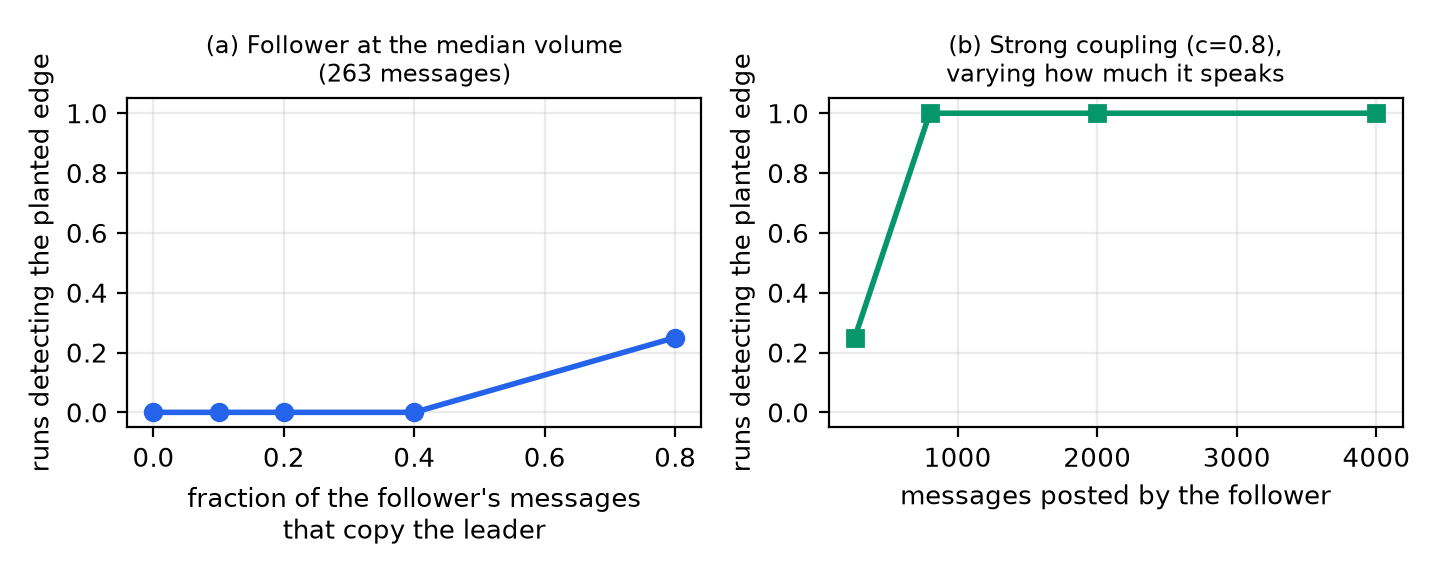
\includegraphics[width=0.92\textwidth]{f4_power.png}
\caption{Detection of a planted follower under the repaired surrogate. Left, varying the fraction of
its messages that copy the leader, at the median agent's volume. Right, varying how much it speaks,
at strong coupling.}
\end{figure}

\paragraph{Humans in the channel.} Main-village \#general is now effectively human-free, with 3 human
messages in the window, so the question has to be asked in open-chat, where 32\% of messages come
from 124 human visitors. Pairwise, with humans collapsed into one node, 19 edges are certified.
Conditioning removes almost all the agent-to-agent structure and little of the rest: \textbf{four
edges survive, of which three run from humans to agents, one is agent to agent, and none run from an
agent to a human.} The asymmetry is not an artifact of the confound. It should be read carefully all
the same: topical dependence from a person to an agent is also what ordinary responsiveness looks
like, so the measurement supports only that the dependence is dyad-specific and directional, not
that anyone is steering a swarm.

\section{Reproducibility, and one limitation of it}

Every number in this paper is recomputed from committed analysis output by a verifier that fails on a
mismatch, and that verifier covers the prose of this paper as well as the figures.

One limitation should be stated plainly. Re-running the counts in the earlier stationarity sweep with
the same seeds and configuration, only one of the eight cells reproduced exactly; the remaining
differences were one or two replicates per cell. Seven of the eight published rates still fell within
the recomputed Wilson intervals, and no conclusion changed. The exception is the zero-drift cell under
the permutation null, where the published 1 of 30 falls just below the recomputed interval of
$[0.035, 0.256]$ for 3 of 30, and no result here depends on that cell.

The generator, estimator and BLAS configuration were investigated and ruled out as the source. The
most likely explanation is a library-level difference, particularly in scikit-learn's $k$-means
implementation within the symboliser, whose output can vary between versions. Every sweep now records
the environment it ran under: Python 3.14.6, numpy 2.5.1, scipy 1.18.0 and scikit-learn 1.9.0,
including the BLAS build and the number of BLAS threads each worker used.

This does not make the previously published counts exactly reproducible. It provides a more clearly
specified environment in which subsequent results can be checked. For that reason I report rates
alongside their confidence intervals rather than exact replicate counts. The distinction between
reproducing a result within its uncertainty and reproducing every individual count matters, and only
the first is claimed.

\section{Conclusion}

Applied to real agent chat, the standard recipe for ``who drives whom'' needs repair before it says
anything. Clock windows cannot separate a message from its answer at the speed agents reply, and what
they certify is matched by a null with no access to meaning. The turn-ordered grid that fixes this
breaks the circular-shift surrogate: family-wise error 0.90 against a nominal 0.05, caused by the
speaker sequence itself. Restricted permutation surrogates repair most of that, but they are flat
under drift rather than calibrated, they are mutually indistinguishable at this precision, and one of
them needs twice the surrogate draws anyone would think to use. A valid surrogate fixes calibration
but not confounding. What survives is small: two dyad-specific edges that do not replicate, an
undetermined answer set by conditioning resolution, and influence running from people into agents and
never back. \textbf{An influence graph should not guide decisions until its error rate, its confound,
its detection floor and its symboliser's fidelity are reported.}

\section*{Limitations}

\begin{itemize}
\item \textbf{Immediate-predecessor only.} The turn-ordered lag-1 measure sees influence from the
message directly before a reply. Influence acting over several turns, or through a room's accumulated
context, is out of scope.
\item \textbf{Discrete approximation to an event process.} Agent chat is event-based in continuous
time. The turn-ordered discretisation with a permutation surrogate is a practical fix, and the
continuous-time comparison above shows what that choice gives up.
\item \textbf{The mechanism behind the real 0.90 is not established.} The generator separates
turn-taking from drift and points at drift, but the largest cell anywhere in the design is 0.365.
\item \textbf{Symbolisation quality cannot be measured on the real logs.} The central result survives
an independent symboliser, but the edge count does not: it moves with alphabet size and with which
messages the topic model is fit on. The floor remains the largest unquantified threat.
\item \textbf{No ground truth in the real logs.} The validity argument rests on planted controls and
on the meaning-free null, not on recovering a known answer.
\item \textbf{Conditioning removes real influence too.} The conditional estimate discards influence
that works by shifting what the channel is talking about, which in a group chat may be a large part
of genuine influence. It is a lower bound on dyadic influence.
\item \textbf{The human result is exploratory.} It rests on one village and one window and should be
read as a lead.
\end{itemize}

\section*{Broader impact and ethics}

This work audits influence detection on a population of AI agents, which is dual-use. Used
defensively it helps an overseer decide what an influence graph is worth, and the main result is
deflationary: it tells practitioners to trust these outputs less, which reduces rather than increases
the chance of acting on a bad attribution. The same tooling could be used to identify the most
influential agent in a swarm in order to target it, or to surveil participants in a channel. Three
properties limit the misuse. The subjects are AI models; the dataset is already public under research
terms and no re-identification is added; and the measure is weak and local, recovering
immediate-predecessor topical dependence rather than any model of how to steer an agent.

The dataset's research terms were followed: research use only, no training on the data, no
re-identification, citation of the source, and notification of the authors of resulting publications.
Human participants appear only as an aggregate node or as anonymised visitor labels, never by name or
handle, and no content attributable to an individual person is reported. Message text and metadata
were read, never model weights or private user data.

The use of a large language model in this work is disclosed in the first-page footnote, as TMLR
requires.

\bibliographystyle{tmlr}
\bibliography{refs}

\end{document}
"               camera-ready
% Use build.py, which runs all of them and checks the anonymous output for leaks.
\providecommand{\TMLRMODE}{submission}
\makeatletter
\def\@tmlrpreprint{preprint}
\def\@tmlraccepted{accepted}
\ifx\TMLRMODE\@tmlrpreprint
  \usepackage[preprint]{tmlr}
\else
  \ifx\TMLRMODE\@tmlraccepted
    \usepackage[accepted]{tmlr}
  \else
    \usepackage{tmlr}
  \fi
\fi
\makeatother

\usepackage{hyperref}
\usepackage{url}
\usepackage{booktabs}
\usepackage{graphicx}
\usepackage{amsmath}

% Gate every identifying string on whether identity may be revealed at all. The flag to test is
% \if@accepted, NOT \if@preprint: tmlr.sty's [preprint] option sets BOTH, so \if@accepted is true
% for the preprint and the camera-ready and false only for the anonymous submission, which is
% exactly the condition wanted. Gating on \if@preprint alone also hid the repository URLs from the
% camera-ready, which is where this paper promises to give them. \if@accepted is internal to
% tmlr.sty, hence the \makeatletter. The anonymous build takes the second argument.
\makeatletter
\newcommand{\ifdeanon}[2]{\if@accepted#1\else#2\fi}
\makeatother
\newcommand{\benchname}{\ifdeanon{SwarmInfluence-Bench}{the benchmark}}

% An unmarked footnote, for the LLM-use disclosure. TMLR's FAQ requires the disclosure and names
% the location: authors must "mention explicitly in their submission that they have used this
% tool", "as a footnote on the first page". Verified against jmlr.org/tmlr/faq.html on 10 Nov 2026.
% It is therefore not optional, and it does not belong in Broader Impact, where it sat until now.
% Nothing in the policy asks for the vendor's name, so none is given.
\newcommand{\disclosurefootnote}[1]{%
  \begingroup\renewcommand\thefootnote{}\footnote{#1}\addtocounter{footnote}{-1}\endgroup}

\title{An Influence Graph Over AI Agents Certifies an Agent That Copies Nobody}

% Hidden by the tmlr package unless [accepted] or [preprint] is given.
\author{\name Manu Nicholas Jacob \email manunicholasjacob@gmail.com \\
        \addr Independent Researcher}

\def\month{11}
\def\year{2026}
\def\openreview{\url{https://openreview.net/forum?id=XXXXXXXXXX}}

\begin{document}
\maketitle

\begin{abstract}
Circular-shift surrogates can produce severely inflated false-positive rates when applied to
turn-ordered multi-agent conversations, reaching a family-wise error rate of 0.90 against a nominal
0.05. A generated benchmark separates two candidate mechanisms and points at non-stationary speaker
activity rather than turn-taking, which suppresses the failure rather than causing it. No setting of
either knob reproduces the observed 0.90, however, so what drives the full real-data failure remains
open. Restricted permutation surrogates substantially reduce the problem. Their error rate is flat
with respect to drift rather than at the nominal level, and for the global within-speaker variant it
depends on how many surrogate draws the null is built from. Calibration alone does not address
confounding, which motivates a conditional estimator validated against a benchmark with planted
ground truth. I also identify a symbolisation-dependent detection limit and develop label-free
diagnostics for it, and show that their calibration does not transport across degradation
mechanisms. The benchmark is released.
\end{abstract}

\disclosurefootnote{\textbf{Use of a large language model.} A large language model was used as an
assistive tool: to help write and run the analysis code, and to help draft this paper. The author is
responsible for every claim, number and figure. All results come from the released code run on the
public dataset, no result or reference is fabricated, and every number in this paper is recomputed
from committed analysis output by a verifier that fails the build on a mismatch.}

\section{Introduction}

When AI agents interact in a shared channel, it is useful to understand how they influence one
another. Information-theoretic methods offer a way to measure this through lagged transfer entropy,
surrogate testing, and per-agent influence scores. They are attractive because they require no
labels and no access to model internals, only a record of who said what and when. The reliability of
those measurements is what this paper examines.

Almost every demonstration of these detectors runs on synthetic traces with a planted leader, where
the analyst controls timing and vocabulary. Real agent chat is asynchronous, bursty, and written in
open language. The narrower question here is whether the standard recipe, applied to real agent
logs, returns anything an overseer should act on.

The audit runs on the AI Village corpus \citep{aidigest2026}, in which frontier models share chat
channels over eighteen months across four villages differing in size, lifetime and tempo, applying
the checks a reader should demand: planted controls, a meaning-free symboliser, replication in a
held-out window, and sensitivity to every parameter that had to be chosen.

\begin{enumerate}
\item The conventional circular-shift surrogate is \textbf{invalid} on turn-ordered agent chat: a
family-wise error rate of 0.90 against a nominal 0.05, caused by the structure of the speaker
sequence itself.
\item Restricted permutation surrogates restore most of the calibration, and re-certifying under one
\textbf{scrambles rather than shrinks} the answer: one channel loses all 11 of its edges, another
gains 15.
\item The three restricted variants are \textbf{mutually indistinguishable} at the precision reached
here, so the choice between them cannot be justified on error rate. The global within-speaker
variant additionally needs on the order of 200 surrogate draws, and over-fires by roughly a factor
of two at 100.
\item Calibration is not confounding, so a conditional estimate is added and validated on a released
benchmark with a known influence graph: common-cause false edges fall from 22.3 to 0.33, and on the
planted-edge instances precision rises from 0.17 to 0.80 with no loss of recall or power.
\item The same benchmark exposes a \textbf{symbolisation floor}. Below roughly 0.44 adjusted Rand
index between symboliser and truth, detection collapses whatever the estimator. Label-free
diagnostics detect that floor, but their calibration does not transport across degradation
mechanisms, and I report where it fails.
\item On the real channels two edges stand at every conditioning resolution, 18 are
\textbf{undetermined} between 0 and 13, none replicates out of sample, and what survives alongside
humans runs from people to agents.
\end{enumerate}

\section{Related work}

\paragraph{Transfer entropy and surrogates.} Transfer entropy \citep{schreiber2000} measures how much
a source's past reduces uncertainty about a target's next symbol beyond the target's own past.
Plug-in estimators are biased upward on short series, so significance rests on surrogate data, with
family-wise error controlled by a max-T test \citep{westfall1993}. The usual surrogate is a circular
time shift of the source.

\paragraph{Event-based data breaks the shift surrogate.} \citet{shorten2021}, on neural spike trains,
show that the conventional source-time-shift surrogate fails to represent the null hypothesis of
conditional independence for event-based processes, and adapt to that setting the nearest-neighbour
local permutation scheme of \citet{runge2018}. Agent chat is event-based in that sense: messages are
events in continuous time, not samples of a clocked signal. The correction is not a contribution of
this paper. The contribution is showing that the same failure carries over to multi-agent safety
monitoring, and that it can be severe enough to create apparent leaders where none exist.

\paragraph{The same failure, concurrently, in multi-agent reinforcement learning.}
\citet{papadopoulos2026} report a closely related surrogate failure in multi-agent
reinforcement-learning action series. Their agent pairs have zero influence by construction, yet
circular time shifts produce false-positive rates of 100\% and 98.2\% against a nominal 0.05. A
plain permutation surrogate fares no better in their setting, at 100.00\% and 99.95\%. Their
proposed correction restricts permutations to blocks of training time, which returns the rates to
5.25\% and 5.50\%.

There are important differences between their setting and this one. Their data consist of binary
actions recorded over twelve thousand training rounds, whereas these data are symbolised
natural-language messages arranged on a turn-ordered conversational grid. Their non-stationarity
comes from monotone drift associated with annealing exploration; here the relevant non-stationarity
appears in the speaker sequence. Neither result should be taken as a direct extension of the other.

Nevertheless, the fact that both approaches rely on restricted permutations is worth noting. Their
permutation blocks are defined by training time, while mine are defined by an agent's own speaking
positions. This provides convergent evidence that unrestricted temporal rearrangement can be
problematic in non-stationary multi-agent data. Their findings also serve as a useful warning for
the approach taken here, and the warning has a measured form rather than a rhetorical one: in their
data the unrestricted permutation failed as completely as the time shift, at 100.00\% against a
nominal 0.05. Permutation-based surrogates are not automatically protected against
non-stationarity, and what protects the one used here is the restriction, not the permutation. I
claim no priority over their result and view the two studies as complementary, addressing different
forms of structured multi-agent data.

\paragraph{Oversight under a budget.} AI-control research frames monitoring as resource constrained,
with a cost for false positives \citep{greenblatt2024}. An influence graph is one such measurement,
and its error rate is the concern here.

\paragraph{Clustering stability.} The idea of using clustering stability as a label-free quality
indicator is not new. It has a substantial history, including \citet{benhur2002},
\citet{lange2004}, von Luxburg's review of clustering stability \citep{vonluxburg2010}, and
\citet{tibshirani2005} on prediction strength. What is different in Section~\ref{sec:floor} is the
calibration of these diagnostics against a detection-performance floor rather than against cluster
recovery alone.

\section{Data and representation}

The AI Village dataset ships one gzipped-JSONL table per village. Four villages are used, differing
enough to test whether any finding is a property of one channel.

\begin{table}[h]
\centering
\begin{tabular}{lrrrrl}
\toprule
village & agent messages & agents & lifetime & human messages & busiest room \\
\midrule
main      & 205,726 & 58  & 576 days & 10,029 & \#general (166,715, 81\%) \\
open-chat &  35,483 & 23  &  66 days & 12,264 & \#general (all) \\
swarm     &   3,848 & 133 &   1 day  &      5 & room a (3,846) \\
game-jam  &     838 & 6   &   3 days &     36 & per-team rooms \\
\bottomrule
\end{tabular}
\caption{The four villages. A 2026 scaffolding change scopes each agent to its current room's
context, so the busiest room of each village is a self-contained influence substrate and is analysed
alone.}
\end{table}

The primary window is the final fourteen days of main-village \#general, 17 to 31 October 2026,
holding 8,800 agent messages. Twenty-two models posted at least 50 messages each and the directed
test uses the 15 busiest, giving 7,958 message events. Two scaffolding facts are disclosed rather
than corrected: the automated nudger was off throughout, and the unused \#best and \#rest rooms were
soft-deleted mid-window, which does not touch \#general.

\subsection{From open language to symbols}

Transfer entropy needs discrete symbols, so each message is mapped to a small alphabet before
influence is estimated, and that mapping is kept separate from the estimator. A topic symboliser
(TF-IDF then $k$-means, $k=8$) gives a message its topic cluster id, so paraphrases of one idea share
a symbol. A hash symboliser, a stable hash of the normalised text into $k=8$ buckets, has no notion
of meaning and serves as a null: an edge appearing under both lives in timing alone.

\subsection{The lag problem, and why clock windows cannot solve it}

A lag-1 transfer entropy compares window $t-1$ with window $t$, so influence landing inside one
window is invisible to it. Agent chat makes this binding. Among the fifteen analysed agents the gap
between consecutive messages by different speakers has a median of 28.1 seconds (25th percentile
9.2, 75th 66.2, 95th 159.3), so turn-taking is a seconds-scale process while any clock window wide
enough to hold two speakers is minutes wide and swallows both a message and its answer.

Both horns are measurable. At 30 seconds only 1.2\% of agent-windows hold a message, while 32.0\% of
replies already land in the same window as what they answer, rising to 84.4\% at five minutes. At
every width tried, the meaning-free hash null certifies comparably many edges, and more at five
minutes: 9 against 12 at thirty seconds, 17 against 19 at one minute, 27 against 44 at fifteen, and
19 against 17 at five. Whatever clock-window transfer entropy was detecting there, it was not shared
meaning.

\begin{figure}[h]
\centering
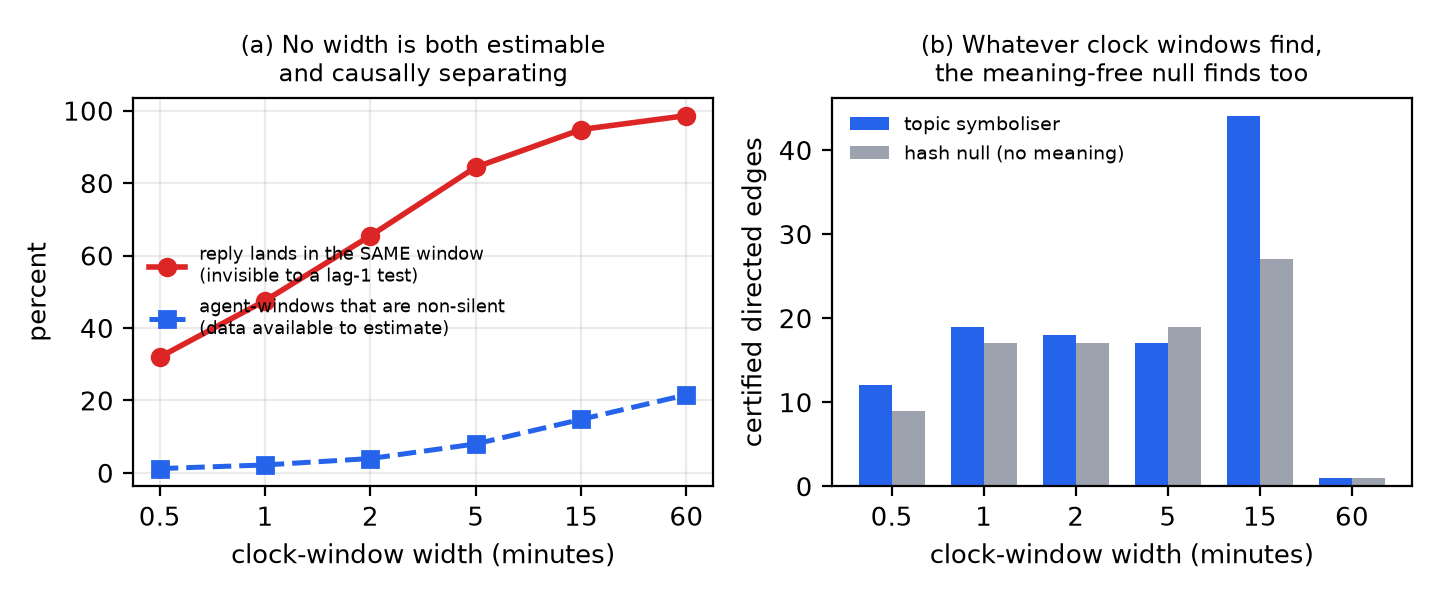
\includegraphics[width=0.92\textwidth]{f1_clock.png}
\caption{Clock-window transfer entropy on the 15 analysed agents of main-village \#general. Left,
the two failure modes as a function of window width. Right, edges certified under the topic
symboliser against the meaning-free hash null.}
\end{figure}

The bind is avoided by ordering messages canonically and letting one message be one tick. Each
agent's series carries its symbol where it spoke and a silent symbol elsewhere, so the lag-1
comparison is between a message and the one immediately before it. The cost is that the measure
captures immediate-predecessor influence only.

\section{The surrogate failure, and two explanations that did not hold}
\label{sec:failure}

An agent is planted into the real stream, drawing its symbols from the channel's marginal and
coupled to nothing at all. It is certified as driving something in 3 of 8 runs when it posts 50
messages, and in 8 of 8 at 100, 263, 600 and 1500 messages, with the mean largest $z$ rising from 5.6
to 12.3, 21.7, 38.3 and 71.7. The error grows with how much the agent speaks, which rules out a
small-sample explanation.

A planted agent could be dismissed as artificial, so the error rate is also measured directly.
Keeping the real speaker sequence and permuting the symbols globally leaves data with no directed
topical influence by construction. The shift surrogate certifies at least one edge in 9 of 10 such
replicates, a family-wise error rate of 0.90 against a nominal 0.05.

\paragraph{What breaks it is the speaker sequence.} Destroying one structure at a time isolates the
cause. Keeping the real speaker order and shuffling only symbols, the shift surrogate fires in 10 of
10 replicates; randomising the speaker order as well drops it to 0 of 10; uniform symbols with the
real order still give 6 of 10. So the driver is the structure of the speaker sequence, not the
symbol distribution and not sparsity. That sequence is far from random in two ways at once: it
repeats a speaker 36\% of the time and returns after one message 38\% of the time, and each agent's
activity is strongly non-stationary, with a median block-share coefficient of variation of 0.79.
Shuffling the order destroys both at once, so this ablation cannot say which of the two mattered.

\subsection{Two explanations I proposed, and the benchmark refuted both}

I initially attributed the failure to mutual exclusivity: only one agent can speak at each tick, so
shifting individual timelines could create overlaps that never occurred in the original
conversation. The benchmark did not support this explanation. A generated channel with exactly one
speaker per tick and steady activity produced an error rate of just 0.025, 95\% Wilson
$[0.011, 0.057]$, far below the 0.90 observed in the real data. Mutual exclusivity alone therefore
cannot explain the failure.

I then suspected turn-taking. In the real channel, speakers repeat 36\% of the time and return after
exactly one message 38\% of the time. However, adding a Markov speaker chain to the generator
produced the opposite result. Turn-taking suppressed the error rather than increasing it. At the
nominal knob values and with no drift the surrogate certified nothing at all across 200 replicates,
while removing turn-taking and introducing drift raised the rate to 0.365. The contribution from
drift was $+0.340$, compared with $-0.025$ for turn-taking. The same inversion appears in the arm
calibrated so that the generated channel reproduces the real channel's measured repeat, return and
block-share statistics rather than merely carrying those numbers as settings: there, turn-taking
alone also certifies nothing, and drift alone gives 0.065.

Neither mechanism, nor their combination in the tested design, reproduced the real-data error rate of
0.90. The largest cell anywhere in the design is 0.365. The real-data ablation removes turn-taking
and non-stationarity together, while the generator separates them. The results point to
non-stationary activity, but the remaining gap means the mechanism behind the full real-data failure
is not yet established.

Every figure above comes from the run at 200 surrogate draws. The first version of this analysis
used 100, which inflates both nulls on the same 2,400 instances: the circular shift fires 53 times
where the 200-draw run does not, against 18 the other way (exact McNemar $p = 3.9 \times 10^{-5}$),
and the permutation surrogate 83 against 20 ($p = 2.7 \times 10^{-10}$). Every qualitative conclusion
in this section is the same at both settings, which is why they are worth stating at all. The
numbers are not, so the draw count belongs in the caption.

\section{The repair, compared}
\label{sec:repair}

Following the local-permutation idea of \citet{runge2018} as adapted by \citet{shorten2021}, each
source keeps its speaking positions and only its symbols are permuted among them. Speaking pattern,
sparsity and turn-taking are preserved exactly, and only the correspondence between symbol and time
is destroyed. On the same destroyed-structure real data the family-wise error rate falls to 0.063
over 300 replicates, 95\% Wilson $[0.041, 0.097]$. The planted uncoupled agent is never certified: 0
of 5 at both 263 and 1500 messages, with mean max $z$ of 2.8 in each case against 22.0 and 68.3
under the shift surrogate.

\begin{figure}[h]
\centering
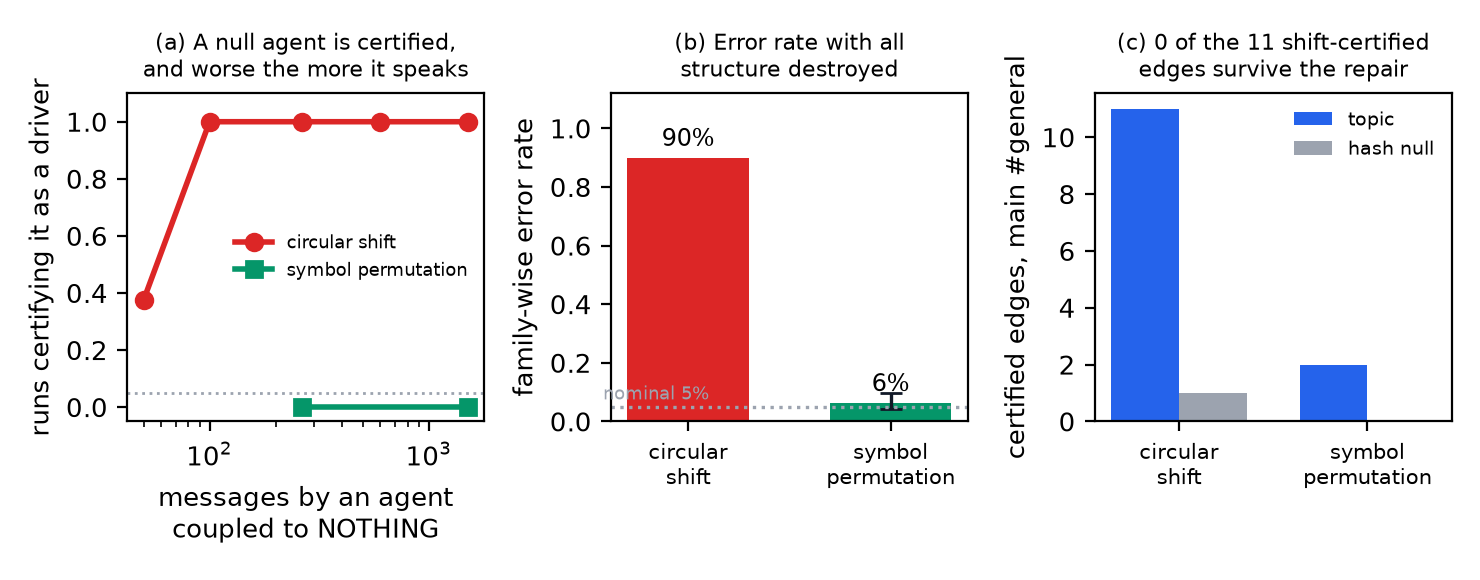
\includegraphics[width=\textwidth]{f2_null.png}
\caption{Left, how often an agent coupled to nothing is certified as a driver, under each surrogate.
Middle, family-wise error rate measured on data with all structure destroyed, with a Wilson
interval; the dotted line is the nominal 0.05. Right, what each surrogate certifies on the real
channel.}
\end{figure}

\subsection{How many surrogate draws are needed}

The number of surrogate draws matters more than I initially appreciated. In a paired comparison of
300 instances, where all four surrogates run on identical symbol grids so the outcomes are paired,
the global permutation surrogate produced a false-positive rate of 0.1167 with 100 draws, falling to
0.0700 with 200 draws, 95\% Wilson $[0.046, 0.105]$. This difference is statistically significant
(exact McNemar $p = 0.0043$). The block-local and Runge local permutations were less sensitive to the
increase: their corresponding rates changed from 0.0900 to 0.0767 and from 0.0967 to 0.0800.

At 200 draws, the global permutation's interval covers the nominal 0.05 and overlaps the real-data
estimate of 0.0633 $[0.0409, 0.0968]$. The real-data result is therefore corroborated rather than
overstated. For practical use, the important point is that reducing the number of surrogate draws
can materially change the result. In particular, the global permutation over-fires at 100 draws by
approximately a factor of two. I would therefore not treat the choice of draw count as a minor
computational detail.

The same correction applies to the benchmark-wide estimate. That figure was 0.0942 at 100 draws.
Repeating all 2,400 instances at 200 draws gives \textbf{0.0679}, 95\% Wilson $[0.0585, 0.0787]$,
and the paired difference is large: 83 instances fire at 100 draws and not at 200, against 20 the
other way, $p = 2.7 \times 10^{-10}$. The conclusion it supports is unchanged, because the interval
still excludes the nominal 0.05. So the permutation repair does carry a residual inflation on clean
generated data, but it is about a third above nominal rather than nearly double.

One limit on this recommendation. I compared 100 draws against 200 and did not test any larger
value, so what the experiment establishes is that 100 is too few, not that 200 is enough. Two
hundred is a lower bound on the draw count rather than a converged setting, and a practitioner whose
conclusions sit near a decision boundary should check their own sensitivity rather than adopt the
number.

\subsection{Choosing a repair, when the error rate cannot choose}

The comparison of the three permutation-based repairs does not produce a clear winner. All four
surrogates were evaluated on identical symbol grids across 300 pure-null replicates, so the
comparison reflects differences between the null models rather than differences between datasets.

\begin{table}[h]
\centering
\begin{tabular}{lrrrl}
\toprule
surrogate & FWER, 100 draws & FWER, 200 draws & 95\% Wilson at 200 & nominal 0.05 \\
\midrule
circular shift                   & 0.0433 & \textbf{0.0333} & $[0.018, 0.060]$ & inside \\
global within-speaker permutation & 0.1167 & \textbf{0.0700} & $[0.046, 0.105]$ & inside \\
block-local permutation          & 0.0900 & \textbf{0.0767} & $[0.052, 0.112]$ & excluded \\
local permutation \citep{runge2018} & 0.0967 & \textbf{0.0800} & $[0.054, 0.116]$ & excluded \\
\bottomrule
\end{tabular}
\caption{Four surrogates on identical symbol grids, 300 pure-null replicates, at both draw counts.}
\end{table}

At 200 draws, paired on the same 300 instances, the circular shift is not significantly different
from the global permutation ($p = 0.0614$), although it differs from block-local permutation
($p = 0.0294$) and from Runge's local permutation ($p = 0.0201$). At 100 draws it differed from all
three, which is the draw-count artifact again. The three repairs remain statistically
indistinguishable from one another, with pairwise $p$-values of 0.85, 0.65 and 1.00. The apparent
differences in their error rates are not sufficient to establish a ranking.

Choosing between them therefore requires more than calibration, and two readings pull against each
other. Runge's local permutation has the strongest methodological justification for preserving the
structure it is intended to preserve, and it follows the approach adapted to event data by
\citet{shorten2021}. Block-local permutation is more heuristic and introduces a free parameter that
has not been tuned. Global permutation is the simplest. On the other hand, the global permutation has
the most favourable interval relative to the nominal rate, and is the only repair that costs nothing
measurable against the shift on clean stationary data, although neither difference is statistically
established. I do not consider the observed error rates sufficient to select one repair over the
others. The choice should be guided by the structure the null is intended to preserve and the
assumptions that can be justified for the data.

\subsection{When to use the repair}

A drift sweep gives the practical reading. Across 150 replicates per cell at 200 surrogate draws,
the circular shift degrades steadily as activity drift increases while the three repairs do not.

\begin{table}[h]
\centering
\begin{tabular}{lrrrr}
\toprule
activity drift & circular shift & global permutation & block-local & local \\
\midrule
0.0 & \textbf{0.013} & 0.093 & 0.080 & 0.093 \\
0.3 & 0.100 & 0.100 & 0.093 & 0.120 \\
0.6 & \textbf{0.193} & 0.053 & 0.047 & 0.067 \\
0.9 & \textbf{0.380} & 0.087 & 0.080 & 0.080 \\
\bottomrule
\end{tabular}
\caption{Family-wise error on pure nulls as activity drift increases, 150 replicates per cell, 200
surrogate draws. Every certified edge is a false positive by construction.}
\end{table}

The pattern is supported by a formal trend test rather than by eye. A Cochran-Armitage test across
the four ordered drift levels gives the circular shift $z = 8.667$, $p < 10^{-15}$, and gives every
repair nothing: $p = 0.51$ for the global permutation, 0.63 for block-local and 0.37 for local. The
same pattern holds at both surrogate draw counts, so it does not depend on that choice.

The repairs are therefore flat under drift rather than calibrated. Only one of the four global
permutation intervals covers the nominal 0.05, and the rest sit nearer 0.09, so what the repair buys
is insensitivity to drift rather than correctness. One asymmetry should be stated rather than
hidden: block-local covers nominal in three of the four cells where the global repair covers one.
The two remain pairwise indistinguishable, so this is not grounds to switch the recommendation, but
it does mean the global repair cannot be described as the best-calibrated under drift.

The results also show why the repair should not be treated as universally preferable. At zero drift
the circular shift has an error rate of 0.013, while the three repairs are all around 0.08 to 0.09.
That advantage is gone by the first drift step: at drift 0.3 the shift reads 0.100 against the global
permutation's 0.100 and block-local's 0.093, so the crossover falls between drift 0.0 and 0.3 rather
than at some higher level. By drift 0.6 the shift is roughly four times the repairs. If a channel has
been checked and found stationary, the circular shift may be sufficient. When activity is
non-stationary the repairs are the more stable choice, and the margin for error on that judgement is
narrow, because the crossover arrives by the first drift level tested.

\section{Continuous time, and what the repair cannot test}

An earlier analysis identified continuous-time estimation as the principled option for event data
but did not evaluate it. Running the continuous-time estimator CoTETE on both channels certifies 0
edges in either case, compared with 2 for main-village and 18 for open-chat under the discrete,
turn-ordered analysis. Its highest $z$-scores are 3.062 and 3.980, below the respective max-T
thresholds of 4.171 and 4.308.

At first these results might appear to contradict the symbol-based analysis. The two estimators
operate on different information, however. CoTETE's public API takes event times with no symbol
channel, while the transfer-entropy analysis here uses topic symbols. To test whether this
difference explains the results, I reduced the data to timing alone, replacing every spoken symbol
with the same code. Under this representation the estimator used here also detects 0 edges in both
channels, matching CoTETE. Using the circular-shift surrogate instead produces 12 and 3 edges. So
neither method detects relationships from event timing alone in these channels, and the edges found
by the symbol-based analysis depend on symbol correspondence, which the continuous-time estimator
cannot access.

Two caveats attach to those $z$-scores, and the second attaches to the larger of them. Point
estimates from this estimator are stochastic to about 17\% across repeated runs, so none of these
values should be read to more than two significant figures. And open-chat's highest $z$, the 3.980,
belongs to the one pair whose surrogate draws mostly failed: it needed 1,936 failed draws to obtain
100 successes, a 4.9\% success rate. Those surrogates are conditioned on being estimable, so that
pair's null is biased in an unknown direction. The conclusion does not rest on it, since that pair
falls below threshold and so does every other pair, but the number should not be quoted as a clean
measurement. The failures themselves were a defect rather than a property of the data: an enlarged
exclusion window can empty the neighbour search on sparse bursty event trains and raise an error
that terminates a whole pair, with no handling at the public entry point. This has been reported
upstream.

There is also a fundamental limitation in applying the recommended permutation surrogate to
timing-only data. When every event carries the same symbol, permuting those symbols changes nothing.
The observed statistic and the surrogate null are identical, making the test exactly degenerate:
standard deviation 0 across all 210 pairs and $p = 1.0$ everywhere. \textbf{The repair has zero power
against timing structure by construction.} The permutation surrogate is appropriate for testing
relationships in the symbol sequence, but it does not answer whether relationships exist in event
timing. These are different questions, and choosing one null means giving up the ability to test the
other with that procedure.

\section{Confounding, and what conditioning removes}

A valid surrogate fixes calibration but not confounding. If every agent tracks a drifting channel
topic, every pair is genuinely dependent through the channel, and pairwise transfer entropy cannot
tell that from direct influence. I therefore also report a \textbf{conditional} estimate, which asks
whether a source's last message adds anything about a target's next one beyond the target's own
history and the channel's recent state. The conditioning variable is the modal symbol of the last
twelve messages, excluding the immediately preceding one so that it does not simply restate the
source.

On a generated benchmark whose decisive instances contain no influence while every agent tracks a
shared drifting topic, so that any certified edge is common cause, pairwise transfer entropy
certifies \textbf{22.3} edges on average and conditioning takes that to \textbf{0.33}, lifting pooled
precision on the four-edge instances from 0.17 to \textbf{0.80} at a recall of 1.0 either way. Across
couplings from 0.05 to 0.8 the conditional test still finds the planted edge in 3 of 3 runs, so the
gain costs no power.

The benchmark flatters the conditional estimator, since its common cause is a shared modal topic and
the conditioning variable is the channel's modal topic. The real channels are harder, and
conditioning there costs degrees of freedom: a 9-symbol alphabet with a 9-valued context gives 6,561
cells against about 7,900 ticks, so that variable is also coarsened to 4 and 2 values.

\begin{table}[h]
\centering
\begin{tabular}{lrrrr}
\toprule
channel & pairwise & conditional, 9 values & 4 values & 2 values \\
\midrule
main \#general      & 2  & \textbf{2, the same two edges} & 2 & 3 \\
open-chat \#general & 18 & \textbf{0} & \textbf{7} & \textbf{13} \\
swarm, room a       & 1  & \textbf{0} & & \\
\bottomrule
\end{tabular}
\caption{Conditioning at three resolutions. Main-village's two edges are robust to that choice;
open-chat's zero is not.}
\end{table}

At the finest resolution the open-chat test is degenerate, its surrogate sitting above the observed
statistic for 65\% of pairs with the largest $z$ in the family only 4.4, so it is failing to reject
rather than finding nothing to reject. Open-chat's structure therefore remains
\textbf{undetermined}: depending on the conditioning resolution, between 0 and 13 of its 18 edges may
survive. That resolution is a free parameter an analyst would set once and never revisit. This is a
property of the channel rather than the estimator: on structure-free real data the conditional test
fires in 2 of 40 replicates, an error rate of 0.05 with a mean $z$ of $-0.001$, so it is nominal
rather than conservative.

\section{The symbolisation floor}
\label{sec:floor}

Everything these methods produce is downstream of turning text into symbols. On the benchmark, where
the underlying topics are known, detection performance drops sharply when agreement between the
symboliser and the ground truth falls below roughly ARI 0.44, and this behaviour appears across the
tested estimators. Importantly, the false-positive rate can look \emph{better} below this point,
because the shared topic structure needed to produce confounded detections is no longer represented
reliably. A pipeline that stops detecting relationships may therefore have lost the signal it needs
rather than become more reliable, and nothing downstream of the symboliser can tell those apart.

\subsection{Detecting the floor without labels}

That degradation can be detected without ground-truth labels. Across the nine-level benchmark sweep,
three statistics separate the below-floor cases with zero errors: seed stability at a threshold of
0.623, agreement with LSA at 0.646, and the Calinski-Harabasz index at 138.9. Seed stability here is
the \textbf{minimum} pairwise agreement across seeds, not the mean; the mean variant makes one error,
at a different threshold of 0.791. Silhouette has the strongest correlation with true ARI, at 0.979,
but is not useful for identifying the boundary because its threshold falls within a gap of just
0.002. A statistic that tracks clustering quality most closely is not necessarily the best one for
making a classification decision.

Error count cannot choose among the three that were perfect, so I tested whether each threshold still
means what it meant when the channel changes for reasons other than topic separability. Applying each
cut unchanged to thirty cells that vary turn-taking, drift, agent count, volume skew, message length
and corpus size, twenty-seven of which hold true ARI at exactly 1.000:

\begin{table}[h]
\centering
\begin{tabular}{lrrrr}
\toprule
diagnostic & cut & errors where fitted & errors, nuisance set & of those at true ARI 1.000 \\
\midrule
seed stability, min across seeds & 0.623 & 0 & 2 & \textbf{0} \\
LSA agreement                    & 0.646 & 0 & 2 & \textbf{0} \\
Calinski-Harabasz                & 138.9 & 0 & 6 & \textbf{3} \\
\bottomrule
\end{tabular}
\caption{Whether a cut fitted on the vocabulary-overlap mechanism survives a change in the channel
that is not a change in topic separability.}
\end{table}

The two bounded statistics err only on the short-message cells, where the symbolisation genuinely has
degraded. Calinski-Harabasz additionally condemns all three cells whose true ARI is exactly 1.000,
for no reason beyond the corpus holding 2,000 messages rather than 8,000, where it reads 76 to 77
against its own cut of 138.9. It is unbounded and grows with sample size, so a published numeric
threshold for it carries no meaning on another corpus. That is why I recommend the two bounded
statistics and not the index that matched them on error count. \textbf{A cut that moves with the
corpus is not a floor cut.}

This is not a weak statistic being discarded on a technicality. Calinski-Harabasz correlates with
true ARI at 0.973, almost as closely as silhouette, and unlike silhouette it classifies the floor
perfectly where it was fitted. It still cannot carry a published threshold. That is the sharper form
of the point above: neither the statistic that tracks quality most closely nor the one that
classifies best on the fitting mechanism is necessarily the one whose cut another researcher can
reuse.

There are important limits to this result. The effective sample size is nine rather than 54, because
the classification label is determined by overlap level. There are no observations between ARI 0.444
and 0.222, so the exact location of the boundary within that interval remains unknown. These
diagnostics classify whether a result is below the tested detection floor; they do not estimate ARI,
and their behaviour is flat between 0.68 and 1.00, and not even monotone there. The benchmark also
uses a single degradation mechanism with a known and correct value of $k$, whereas the true number of
topics in real conversations is unknown. I therefore treat 0.44 as a benchmark-specific, bracketed
result rather than a universal threshold.

\subsection{A contradiction the diagnostic lost}

I initially used these diagnostics to classify one real channel, open-chat, as below the
symbolisation floor. That conclusion did not agree with the channel's measured results: open-chat
certified 18 and 22 edges under the two symbolisers, compared with 2 and 1 for main-village, and its
hash-based null certified zero edges. Rather than treating this disagreement as evidence that the
original measurements were wrong, I revisited the diagnostic itself.

The problem was the choice of $k$. Repeating the comparison with the same channels, loader and window
reproduced the published $k=8$ results to the digit. At $k=4$, however, open-chat reached stability
scores of 0.950 and 0.978, the highest values produced by either channel across the tested settings,
and both exceeded the diagnostic thresholds. The earlier below-floor classification was therefore a
conclusion about one arbitrary choice of $k$, not a reliable statement about the channel. Message
length does not explain the difference either: 27.1\% of main-village messages contain fewer than
five tokens, compared with 2.3\% in open-chat, so the short-message channel is the one the diagnostic
cleared.

This correction changes how the symbolisation results should be read, and it withdrew three claims.

\begin{enumerate}
\item \textbf{The claim that no topic signal remains below the floor is too strong.} The
circular-shift surrogate recovers all four planted edges at every tested overlap level, including
0.95, where ARI is 0.011. The observed collapse is in the permutation null, not necessarily in the
underlying data.
\item \textbf{ARI 0.44 cannot be treated as a universal detection threshold.} When the shared-topic
parameter is 0, detection continues down to ARI 0.296, so the boundary depends on both the
symboliser and the channel.
\item \textbf{Edge counts cannot be used as a measure of symboliser quality.} Even at ARI exactly
1.000, changing the shared-topic parameter alone moves the permutation edge count from 5 to 78.
\end{enumerate}

The diagnostics also do not transfer reliably outside the mechanism on which they were evaluated.
Their balanced accuracy falls from 1.00 to 0.75 and 0.571 under a known mismatch in $k$. All seven
errors made by seed stability are false below-floor classifications, and in every one of those cases
the detector still identifies all planted edges; of the fourteen cells it condemned, eleven had full
conditional recall. The failure direction is the dangerous one: it condemns working symbolisations.

This was an important correction to my own interpretation. I introduced a diagnostic to check whether
the symbolisation was reliable, applied it to the real channels, and found that it contradicted
measurements already in hand. Investigating that contradiction showed the diagnostic was sensitive to
an arbitrary modelling choice. The result is not that the original measurements were wrong, but that
the control was being asked to support a broader conclusion than the evidence allowed. These
diagnostics remain useful within their tested setting, and \textbf{no channel-level floor verdict
should be issued from a single $k$}.

\section{The benchmark}

Real logs have no ground truth, so the common-cause question could not be settled on them. The
generator used here makes the influence graph known by construction: it decides, in code, who speaks
at which tick, on which topic, and who reacts to whom. Surface text is a separate, replaceable layer
drawn from disjoint per-topic vocabularies, so the whole thing runs offline and a detector still has
to symbolise raw text rather than read the labels. Turn-taking and activity drift are independent
knobs, so the two can be varied one at a time, and the generator reproduces its earlier behaviour
bit for bit when both are zero.

\benchname{} is released with 150 tests covering the generator, the detector harness, the text layer,
the floor analysis and the turn-taking factorial.
\ifdeanon{Code and benchmark:
\url{https://github.com/manunicholasjacob/swarm-influence-bench} and
\url{https://github.com/manunicholasjacob/swarm-influence-audit}.}{Code and benchmark are publicly
released; the links are withheld here for anonymity and will be given in the camera-ready version.}

One property of the benchmark must be stated when its numbers are quoted. Planting an edge displaces
other agents' speaking turns, so the generated instances contain real lag-1 dependencies that the
label set does not list. Precision measured against those labels is therefore a \textbf{lower bound}
for any detector, and what the benchmark supports is the comparison between two estimators rather
than the absolute value of either.

\section{What an overseer should do}

Six inexpensive controls should be included whenever an influence graph over an agent channel is
published.

\begin{enumerate}
\item \textbf{Plant an agent coupled to nothing, at your channel's volumes, and check it is not
certified.} This one test would have caught the failure reported here, at one run per volume.
\item \textbf{Measure the error rate directly}, by destroying the structure your method claims to
find and checking the family-wise rate is near nominal. If it is not, your surrogate does not match
your data.
\item \textbf{Preserve the speaker sequence in your surrogate.} Any surrogate that moves an agent's
messages in time will disturb it, and \citet{shorten2021} is the principled route. Use at least 200
surrogate draws, because at 100 the global within-speaker permutation over-fires by roughly a factor
of two.
\item \textbf{Establish the detection floor before interpreting an absence.} ``No edges'' and ``no
influence'' are different claims.
\item \textbf{Condition on the channel, report both numbers, and sweep the resolution.} Pairwise and
conditional bound the answer, and the gap between them is the result. Conditioning costs cells, so
check whether your answer is an artifact of how finely you conditioned. On one channel here it was.
\item \textbf{Report how well your symboliser agrees with the truth, on data where you know it.}
Everything is downstream of turning text into symbols, and below roughly ARI 0.44 detection
collapses whatever the estimator. I have found this control in no influence-detection paper, and it
is also the one that cannot be run on real logs, which is why the floor remains the largest
unquantified threat here.
\end{enumerate}

Two habits follow: publish a meaning-free null's count beside the real one, and require held-out
replication before calling a graph a structure.

\section{The real channels, and what survives}

Re-running every channel under the repaired surrogate changes the answers, and not in one direction.

\begin{table}[h]
\centering
\begin{tabular}{lrrr}
\toprule
channel & window messages & shift: topic / hash & permutation: topic / hash \\
\midrule
main \#general      & 8,800 & 11 / 1 & 2 / 0 \\
open-chat \#general & 8,226 & 3 / 0  & 18 / 0 \\
swarm, room a       & 3,846 & 2 / 1  & 1 / 0 \\
\bottomrule
\end{tabular}
\caption{The same channels under both surrogates, with the meaning-free hash null beside each.}
\end{table}

In main-village, \textbf{none} of the 11 edges the standard recipe certifies survives the repair, and
the two the valid surrogate certifies were not among them. In open-chat the correction runs the other
way, 3 edges becoming 18, because pathological pairs inflate the max-T threshold and raise the bar
for everything else. An invalid surrogate does not simply add false positives; it scrambles the
result.

Main-village's two edges are the strongest thing here and they are still not a finding, because they
do not replicate: the adjacent fourteen-day window certifies nothing at all under either estimator.
Given the detection floor, that silence is as consistent with the test sitting near its limit as with
the edges being absent, and the two cannot be separated. Power is governed by how much an agent says
as much as by how strongly it copies, and it is channel-specific: in main-village a planted follower
copying on 80\% of its messages is caught only 1 time in 4, while in open-chat one copying 10\% of
the time is caught 3 times in 4. Replication is weak everywhere: under the standard recipe the
adjacent window shares 1 edge out of 8 and 4, and that edge is also the only one the hash null
certifies. No certified edge in this work replicates out of sample.

\begin{figure}[h]
\centering
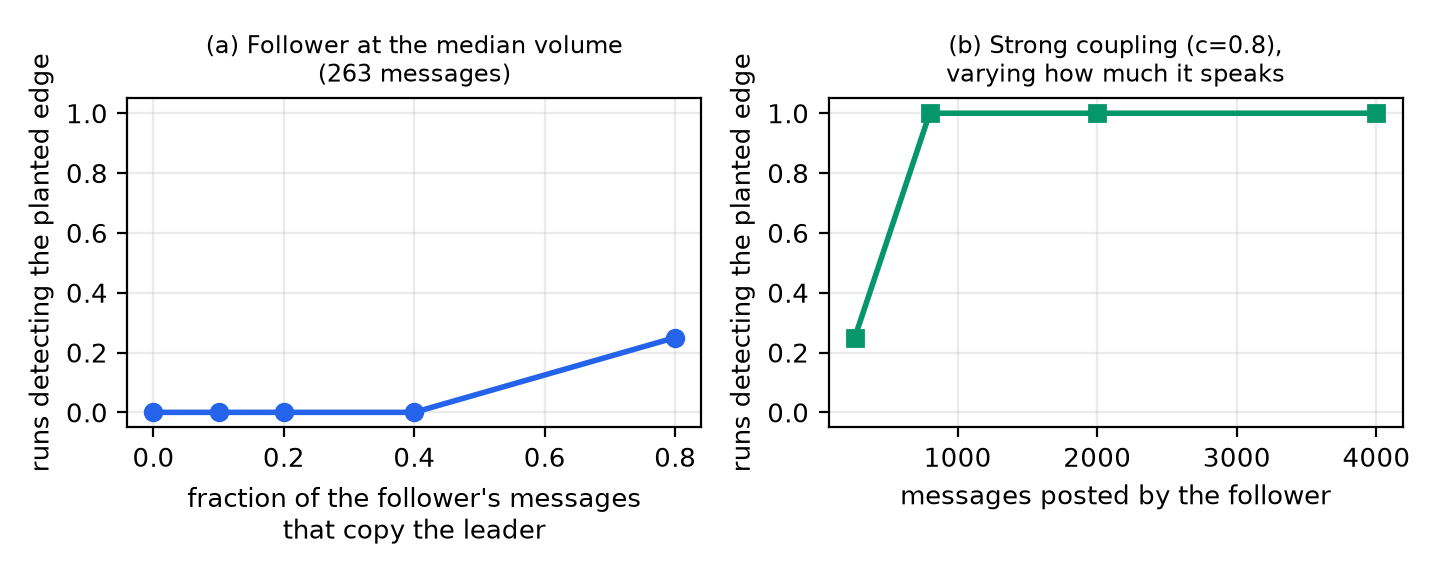
\includegraphics[width=0.92\textwidth]{f4_power.png}
\caption{Detection of a planted follower under the repaired surrogate. Left, varying the fraction of
its messages that copy the leader, at the median agent's volume. Right, varying how much it speaks,
at strong coupling.}
\end{figure}

\paragraph{Humans in the channel.} Main-village \#general is now effectively human-free, with 3 human
messages in the window, so the question has to be asked in open-chat, where 32\% of messages come
from 124 human visitors. Pairwise, with humans collapsed into one node, 19 edges are certified.
Conditioning removes almost all the agent-to-agent structure and little of the rest: \textbf{four
edges survive, of which three run from humans to agents, one is agent to agent, and none run from an
agent to a human.} The asymmetry is not an artifact of the confound. It should be read carefully all
the same: topical dependence from a person to an agent is also what ordinary responsiveness looks
like, so the measurement supports only that the dependence is dyad-specific and directional, not
that anyone is steering a swarm.

\section{Reproducibility, and one limitation of it}

Every number in this paper is recomputed from committed analysis output by a verifier that fails on a
mismatch, and that verifier covers the prose of this paper as well as the figures.

One limitation should be stated plainly. Re-running the counts in the earlier stationarity sweep with
the same seeds and configuration, only one of the eight cells reproduced exactly; the remaining
differences were one or two replicates per cell. Seven of the eight published rates still fell within
the recomputed Wilson intervals, and no conclusion changed. The exception is the zero-drift cell under
the permutation null, where the published 1 of 30 falls just below the recomputed interval of
$[0.035, 0.256]$ for 3 of 30, and no result here depends on that cell.

The generator, estimator and BLAS configuration were investigated and ruled out as the source. The
most likely explanation is a library-level difference, particularly in scikit-learn's $k$-means
implementation within the symboliser, whose output can vary between versions. Every sweep now records
the environment it ran under: Python 3.14.6, numpy 2.5.1, scipy 1.18.0 and scikit-learn 1.9.0,
including the BLAS build and the number of BLAS threads each worker used.

This does not make the previously published counts exactly reproducible. It provides a more clearly
specified environment in which subsequent results can be checked. For that reason I report rates
alongside their confidence intervals rather than exact replicate counts. The distinction between
reproducing a result within its uncertainty and reproducing every individual count matters, and only
the first is claimed.

\section{Conclusion}

Applied to real agent chat, the standard recipe for ``who drives whom'' needs repair before it says
anything. Clock windows cannot separate a message from its answer at the speed agents reply, and what
they certify is matched by a null with no access to meaning. The turn-ordered grid that fixes this
breaks the circular-shift surrogate: family-wise error 0.90 against a nominal 0.05, caused by the
speaker sequence itself. Restricted permutation surrogates repair most of that, but they are flat
under drift rather than calibrated, they are mutually indistinguishable at this precision, and one of
them needs twice the surrogate draws anyone would think to use. A valid surrogate fixes calibration
but not confounding. What survives is small: two dyad-specific edges that do not replicate, an
undetermined answer set by conditioning resolution, and influence running from people into agents and
never back. \textbf{An influence graph should not guide decisions until its error rate, its confound,
its detection floor and its symboliser's fidelity are reported.}

\section*{Limitations}

\begin{itemize}
\item \textbf{Immediate-predecessor only.} The turn-ordered lag-1 measure sees influence from the
message directly before a reply. Influence acting over several turns, or through a room's accumulated
context, is out of scope.
\item \textbf{Discrete approximation to an event process.} Agent chat is event-based in continuous
time. The turn-ordered discretisation with a permutation surrogate is a practical fix, and the
continuous-time comparison above shows what that choice gives up.
\item \textbf{The mechanism behind the real 0.90 is not established.} The generator separates
turn-taking from drift and points at drift, but the largest cell anywhere in the design is 0.365.
\item \textbf{Symbolisation quality cannot be measured on the real logs.} The central result survives
an independent symboliser, but the edge count does not: it moves with alphabet size and with which
messages the topic model is fit on. The floor remains the largest unquantified threat.
\item \textbf{No ground truth in the real logs.} The validity argument rests on planted controls and
on the meaning-free null, not on recovering a known answer.
\item \textbf{Conditioning removes real influence too.} The conditional estimate discards influence
that works by shifting what the channel is talking about, which in a group chat may be a large part
of genuine influence. It is a lower bound on dyadic influence.
\item \textbf{The human result is exploratory.} It rests on one village and one window and should be
read as a lead.
\end{itemize}

\section*{Broader impact and ethics}

This work audits influence detection on a population of AI agents, which is dual-use. Used
defensively it helps an overseer decide what an influence graph is worth, and the main result is
deflationary: it tells practitioners to trust these outputs less, which reduces rather than increases
the chance of acting on a bad attribution. The same tooling could be used to identify the most
influential agent in a swarm in order to target it, or to surveil participants in a channel. Three
properties limit the misuse. The subjects are AI models; the dataset is already public under research
terms and no re-identification is added; and the measure is weak and local, recovering
immediate-predecessor topical dependence rather than any model of how to steer an agent.

The dataset's research terms were followed: research use only, no training on the data, no
re-identification, citation of the source, and notification of the authors of resulting publications.
Human participants appear only as an aggregate node or as anonymised visitor labels, never by name or
handle, and no content attributable to an individual person is reported. Message text and metadata
were read, never model weights or private user data.

The use of a large language model in this work is disclosed in the first-page footnote, as TMLR
requires.

\bibliographystyle{tmlr}
\bibliography{refs}

\end{document}
"               camera-ready
% Use build.py, which runs all of them and checks the anonymous output for leaks.
\providecommand{\TMLRMODE}{submission}
\makeatletter
\def\@tmlrpreprint{preprint}
\def\@tmlraccepted{accepted}
\ifx\TMLRMODE\@tmlrpreprint
  \usepackage[preprint]{tmlr}
\else
  \ifx\TMLRMODE\@tmlraccepted
    \usepackage[accepted]{tmlr}
  \else
    \usepackage{tmlr}
  \fi
\fi
\makeatother

\usepackage{hyperref}
\usepackage{url}
\usepackage{booktabs}
\usepackage{graphicx}
\usepackage{amsmath}

% Gate every identifying string on whether identity may be revealed at all. The flag to test is
% \if@accepted, NOT \if@preprint: tmlr.sty's [preprint] option sets BOTH, so \if@accepted is true
% for the preprint and the camera-ready and false only for the anonymous submission, which is
% exactly the condition wanted. Gating on \if@preprint alone also hid the repository URLs from the
% camera-ready, which is where this paper promises to give them. \if@accepted is internal to
% tmlr.sty, hence the \makeatletter. The anonymous build takes the second argument.
\makeatletter
\newcommand{\ifdeanon}[2]{\if@accepted#1\else#2\fi}
\makeatother
\newcommand{\benchname}{\ifdeanon{SwarmInfluence-Bench}{the benchmark}}

% An unmarked footnote, for the LLM-use disclosure. TMLR's FAQ requires the disclosure and names
% the location: authors must "mention explicitly in their submission that they have used this
% tool", "as a footnote on the first page". Verified against jmlr.org/tmlr/faq.html on 10 Nov 2026.
% It is therefore not optional, and it does not belong in Broader Impact, where it sat until now.
% Nothing in the policy asks for the vendor's name, so none is given.
\newcommand{\disclosurefootnote}[1]{%
  \begingroup\renewcommand\thefootnote{}\footnote{#1}\addtocounter{footnote}{-1}\endgroup}

\title{An Influence Graph Over AI Agents Certifies an Agent That Copies Nobody}

% Hidden by the tmlr package unless [accepted] or [preprint] is given.
\author{\name Manu Nicholas Jacob \email manunicholasjacob@gmail.com \\
        \addr Independent Researcher}

\def\month{11}
\def\year{2026}
\def\openreview{\url{https://openreview.net/forum?id=XXXXXXXXXX}}

\begin{document}
\maketitle

\begin{abstract}
Circular-shift surrogates can produce severely inflated false-positive rates when applied to
turn-ordered multi-agent conversations, reaching a family-wise error rate of 0.90 against a nominal
0.05. A generated benchmark separates two candidate mechanisms and points at non-stationary speaker
activity rather than turn-taking, which suppresses the failure rather than causing it. No setting of
either knob reproduces the observed 0.90, however, so what drives the full real-data failure remains
open. Restricted permutation surrogates substantially reduce the problem. Their error rate is flat
with respect to drift rather than at the nominal level, and for the global within-speaker variant it
depends on how many surrogate draws the null is built from. Calibration alone does not address
confounding, which motivates a conditional estimator validated against a benchmark with planted
ground truth. I also identify a symbolisation-dependent detection limit and develop label-free
diagnostics for it, and show that their calibration does not transport across degradation
mechanisms. The benchmark is released.
\end{abstract}

\disclosurefootnote{\textbf{Use of a large language model.} A large language model was used as an
assistive tool: to help write and run the analysis code, and to help draft this paper. The author is
responsible for every claim, number and figure. All results come from the released code run on the
public dataset, no result or reference is fabricated, and every number in this paper is recomputed
from committed analysis output by a verifier that fails the build on a mismatch.}

\section{Introduction}

When AI agents interact in a shared channel, it is useful to understand how they influence one
another. Information-theoretic methods offer a way to measure this through lagged transfer entropy,
surrogate testing, and per-agent influence scores. They are attractive because they require no
labels and no access to model internals, only a record of who said what and when. The reliability of
those measurements is what this paper examines.

Almost every demonstration of these detectors runs on synthetic traces with a planted leader, where
the analyst controls timing and vocabulary. Real agent chat is asynchronous, bursty, and written in
open language. The narrower question here is whether the standard recipe, applied to real agent
logs, returns anything an overseer should act on.

The audit runs on the AI Village corpus \citep{aidigest2026}, in which frontier models share chat
channels over eighteen months across four villages differing in size, lifetime and tempo, applying
the checks a reader should demand: planted controls, a meaning-free symboliser, replication in a
held-out window, and sensitivity to every parameter that had to be chosen.

\begin{enumerate}
\item The conventional circular-shift surrogate is \textbf{invalid} on turn-ordered agent chat: a
family-wise error rate of 0.90 against a nominal 0.05, caused by the structure of the speaker
sequence itself.
\item Restricted permutation surrogates restore most of the calibration, and re-certifying under one
\textbf{scrambles rather than shrinks} the answer: one channel loses all 11 of its edges, another
gains 15.
\item The three restricted variants are \textbf{mutually indistinguishable} at the precision reached
here, so the choice between them cannot be justified on error rate. The global within-speaker
variant additionally needs on the order of 200 surrogate draws, and over-fires by roughly a factor
of two at 100.
\item Calibration is not confounding, so a conditional estimate is added and validated on a released
benchmark with a known influence graph: common-cause false edges fall from 22.3 to 0.33, and on the
planted-edge instances precision rises from 0.17 to 0.80 with no loss of recall or power.
\item The same benchmark exposes a \textbf{symbolisation floor}. Below roughly 0.44 adjusted Rand
index between symboliser and truth, detection collapses whatever the estimator. Label-free
diagnostics detect that floor, but their calibration does not transport across degradation
mechanisms, and I report where it fails.
\item On the real channels two edges stand at every conditioning resolution, 18 are
\textbf{undetermined} between 0 and 13, none replicates out of sample, and what survives alongside
humans runs from people to agents.
\end{enumerate}

\section{Related work}

\paragraph{Transfer entropy and surrogates.} Transfer entropy \citep{schreiber2000} measures how much
a source's past reduces uncertainty about a target's next symbol beyond the target's own past.
Plug-in estimators are biased upward on short series, so significance rests on surrogate data, with
family-wise error controlled by a max-T test \citep{westfall1993}. The usual surrogate is a circular
time shift of the source.

\paragraph{Event-based data breaks the shift surrogate.} \citet{shorten2021}, on neural spike trains,
show that the conventional source-time-shift surrogate fails to represent the null hypothesis of
conditional independence for event-based processes, and adapt to that setting the nearest-neighbour
local permutation scheme of \citet{runge2018}. Agent chat is event-based in that sense: messages are
events in continuous time, not samples of a clocked signal. The correction is not a contribution of
this paper. The contribution is showing that the same failure carries over to multi-agent safety
monitoring, and that it can be severe enough to create apparent leaders where none exist.

\paragraph{The same failure, concurrently, in multi-agent reinforcement learning.}
\citet{papadopoulos2026} report a closely related surrogate failure in multi-agent
reinforcement-learning action series. Their agent pairs have zero influence by construction, yet
circular time shifts produce false-positive rates of 100\% and 98.2\% against a nominal 0.05. A
plain permutation surrogate fares no better in their setting, at 100.00\% and 99.95\%. Their
proposed correction restricts permutations to blocks of training time, which returns the rates to
5.25\% and 5.50\%.

There are important differences between their setting and this one. Their data consist of binary
actions recorded over twelve thousand training rounds, whereas these data are symbolised
natural-language messages arranged on a turn-ordered conversational grid. Their non-stationarity
comes from monotone drift associated with annealing exploration; here the relevant non-stationarity
appears in the speaker sequence. Neither result should be taken as a direct extension of the other.

Nevertheless, the fact that both approaches rely on restricted permutations is worth noting. Their
permutation blocks are defined by training time, while mine are defined by an agent's own speaking
positions. This provides convergent evidence that unrestricted temporal rearrangement can be
problematic in non-stationary multi-agent data. Their findings also serve as a useful warning for
the approach taken here, and the warning has a measured form rather than a rhetorical one: in their
data the unrestricted permutation failed as completely as the time shift, at 100.00\% against a
nominal 0.05. Permutation-based surrogates are not automatically protected against
non-stationarity, and what protects the one used here is the restriction, not the permutation. I
claim no priority over their result and view the two studies as complementary, addressing different
forms of structured multi-agent data.

\paragraph{Oversight under a budget.} AI-control research frames monitoring as resource constrained,
with a cost for false positives \citep{greenblatt2024}. An influence graph is one such measurement,
and its error rate is the concern here.

\paragraph{Clustering stability.} The idea of using clustering stability as a label-free quality
indicator is not new. It has a substantial history, including \citet{benhur2002},
\citet{lange2004}, von Luxburg's review of clustering stability \citep{vonluxburg2010}, and
\citet{tibshirani2005} on prediction strength. What is different in Section~\ref{sec:floor} is the
calibration of these diagnostics against a detection-performance floor rather than against cluster
recovery alone.

\section{Data and representation}

The AI Village dataset ships one gzipped-JSONL table per village. Four villages are used, differing
enough to test whether any finding is a property of one channel.

\begin{table}[h]
\centering
\begin{tabular}{lrrrrl}
\toprule
village & agent messages & agents & lifetime & human messages & busiest room \\
\midrule
main      & 205,726 & 58  & 576 days & 10,029 & \#general (166,715, 81\%) \\
open-chat &  35,483 & 23  &  66 days & 12,264 & \#general (all) \\
swarm     &   3,848 & 133 &   1 day  &      5 & room a (3,846) \\
game-jam  &     838 & 6   &   3 days &     36 & per-team rooms \\
\bottomrule
\end{tabular}
\caption{The four villages. A 2026 scaffolding change scopes each agent to its current room's
context, so the busiest room of each village is a self-contained influence substrate and is analysed
alone.}
\end{table}

The primary window is the final fourteen days of main-village \#general, 17 to 31 October 2026,
holding 8,800 agent messages. Twenty-two models posted at least 50 messages each and the directed
test uses the 15 busiest, giving 7,958 message events. Two scaffolding facts are disclosed rather
than corrected: the automated nudger was off throughout, and the unused \#best and \#rest rooms were
soft-deleted mid-window, which does not touch \#general.

\subsection{From open language to symbols}

Transfer entropy needs discrete symbols, so each message is mapped to a small alphabet before
influence is estimated, and that mapping is kept separate from the estimator. A topic symboliser
(TF-IDF then $k$-means, $k=8$) gives a message its topic cluster id, so paraphrases of one idea share
a symbol. A hash symboliser, a stable hash of the normalised text into $k=8$ buckets, has no notion
of meaning and serves as a null: an edge appearing under both lives in timing alone.

\subsection{The lag problem, and why clock windows cannot solve it}

A lag-1 transfer entropy compares window $t-1$ with window $t$, so influence landing inside one
window is invisible to it. Agent chat makes this binding. Among the fifteen analysed agents the gap
between consecutive messages by different speakers has a median of 28.1 seconds (25th percentile
9.2, 75th 66.2, 95th 159.3), so turn-taking is a seconds-scale process while any clock window wide
enough to hold two speakers is minutes wide and swallows both a message and its answer.

Both horns are measurable. At 30 seconds only 1.2\% of agent-windows hold a message, while 32.0\% of
replies already land in the same window as what they answer, rising to 84.4\% at five minutes. At
every width tried, the meaning-free hash null certifies comparably many edges, and more at five
minutes: 9 against 12 at thirty seconds, 17 against 19 at one minute, 27 against 44 at fifteen, and
19 against 17 at five. Whatever clock-window transfer entropy was detecting there, it was not shared
meaning.

\begin{figure}[h]
\centering
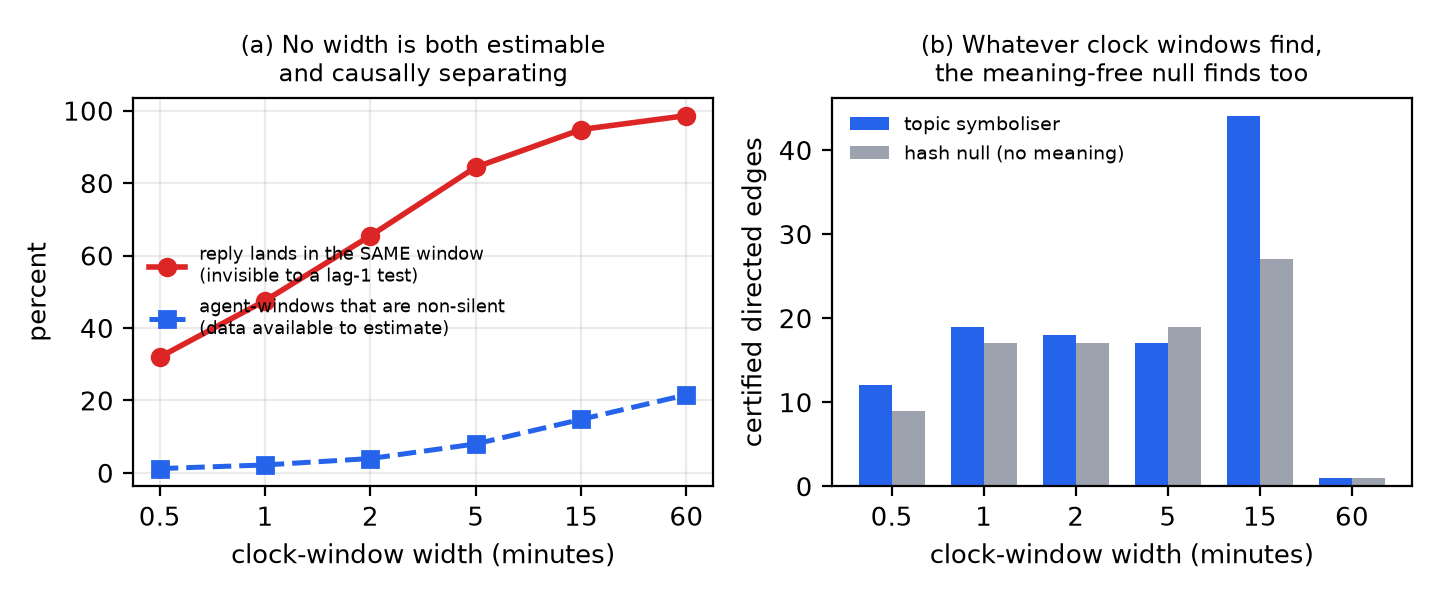
\includegraphics[width=0.92\textwidth]{f1_clock.png}
\caption{Clock-window transfer entropy on the 15 analysed agents of main-village \#general. Left,
the two failure modes as a function of window width. Right, edges certified under the topic
symboliser against the meaning-free hash null.}
\end{figure}

The bind is avoided by ordering messages canonically and letting one message be one tick. Each
agent's series carries its symbol where it spoke and a silent symbol elsewhere, so the lag-1
comparison is between a message and the one immediately before it. The cost is that the measure
captures immediate-predecessor influence only.

\section{The surrogate failure, and two explanations that did not hold}
\label{sec:failure}

An agent is planted into the real stream, drawing its symbols from the channel's marginal and
coupled to nothing at all. It is certified as driving something in 3 of 8 runs when it posts 50
messages, and in 8 of 8 at 100, 263, 600 and 1500 messages, with the mean largest $z$ rising from 5.6
to 12.3, 21.7, 38.3 and 71.7. The error grows with how much the agent speaks, which rules out a
small-sample explanation.

A planted agent could be dismissed as artificial, so the error rate is also measured directly.
Keeping the real speaker sequence and permuting the symbols globally leaves data with no directed
topical influence by construction. The shift surrogate certifies at least one edge in 9 of 10 such
replicates, a family-wise error rate of 0.90 against a nominal 0.05.

\paragraph{What breaks it is the speaker sequence.} Destroying one structure at a time isolates the
cause. Keeping the real speaker order and shuffling only symbols, the shift surrogate fires in 10 of
10 replicates; randomising the speaker order as well drops it to 0 of 10; uniform symbols with the
real order still give 6 of 10. So the driver is the structure of the speaker sequence, not the
symbol distribution and not sparsity. That sequence is far from random in two ways at once: it
repeats a speaker 36\% of the time and returns after one message 38\% of the time, and each agent's
activity is strongly non-stationary, with a median block-share coefficient of variation of 0.79.
Shuffling the order destroys both at once, so this ablation cannot say which of the two mattered.

\subsection{Two explanations I proposed, and the benchmark refuted both}

I initially attributed the failure to mutual exclusivity: only one agent can speak at each tick, so
shifting individual timelines could create overlaps that never occurred in the original
conversation. The benchmark did not support this explanation. A generated channel with exactly one
speaker per tick and steady activity produced an error rate of just 0.025, 95\% Wilson
$[0.011, 0.057]$, far below the 0.90 observed in the real data. Mutual exclusivity alone therefore
cannot explain the failure.

I then suspected turn-taking. In the real channel, speakers repeat 36\% of the time and return after
exactly one message 38\% of the time. However, adding a Markov speaker chain to the generator
produced the opposite result. Turn-taking suppressed the error rather than increasing it. At the
nominal knob values and with no drift the surrogate certified nothing at all across 200 replicates,
while removing turn-taking and introducing drift raised the rate to 0.365. The contribution from
drift was $+0.340$, compared with $-0.025$ for turn-taking. The same inversion appears in the arm
calibrated so that the generated channel reproduces the real channel's measured repeat, return and
block-share statistics rather than merely carrying those numbers as settings: there, turn-taking
alone also certifies nothing, and drift alone gives 0.065.

Neither mechanism, nor their combination in the tested design, reproduced the real-data error rate of
0.90. The largest cell anywhere in the design is 0.365. The real-data ablation removes turn-taking
and non-stationarity together, while the generator separates them. The results point to
non-stationary activity, but the remaining gap means the mechanism behind the full real-data failure
is not yet established.

Every figure above comes from the run at 200 surrogate draws. The first version of this analysis
used 100, which inflates both nulls on the same 2,400 instances: the circular shift fires 53 times
where the 200-draw run does not, against 18 the other way (exact McNemar $p = 3.9 \times 10^{-5}$),
and the permutation surrogate 83 against 20 ($p = 2.7 \times 10^{-10}$). Every qualitative conclusion
in this section is the same at both settings, which is why they are worth stating at all. The
numbers are not, so the draw count belongs in the caption.

\section{The repair, compared}
\label{sec:repair}

Following the local-permutation idea of \citet{runge2018} as adapted by \citet{shorten2021}, each
source keeps its speaking positions and only its symbols are permuted among them. Speaking pattern,
sparsity and turn-taking are preserved exactly, and only the correspondence between symbol and time
is destroyed. On the same destroyed-structure real data the family-wise error rate falls to 0.063
over 300 replicates, 95\% Wilson $[0.041, 0.097]$. The planted uncoupled agent is never certified: 0
of 5 at both 263 and 1500 messages, with mean max $z$ of 2.8 in each case against 22.0 and 68.3
under the shift surrogate.

\begin{figure}[h]
\centering
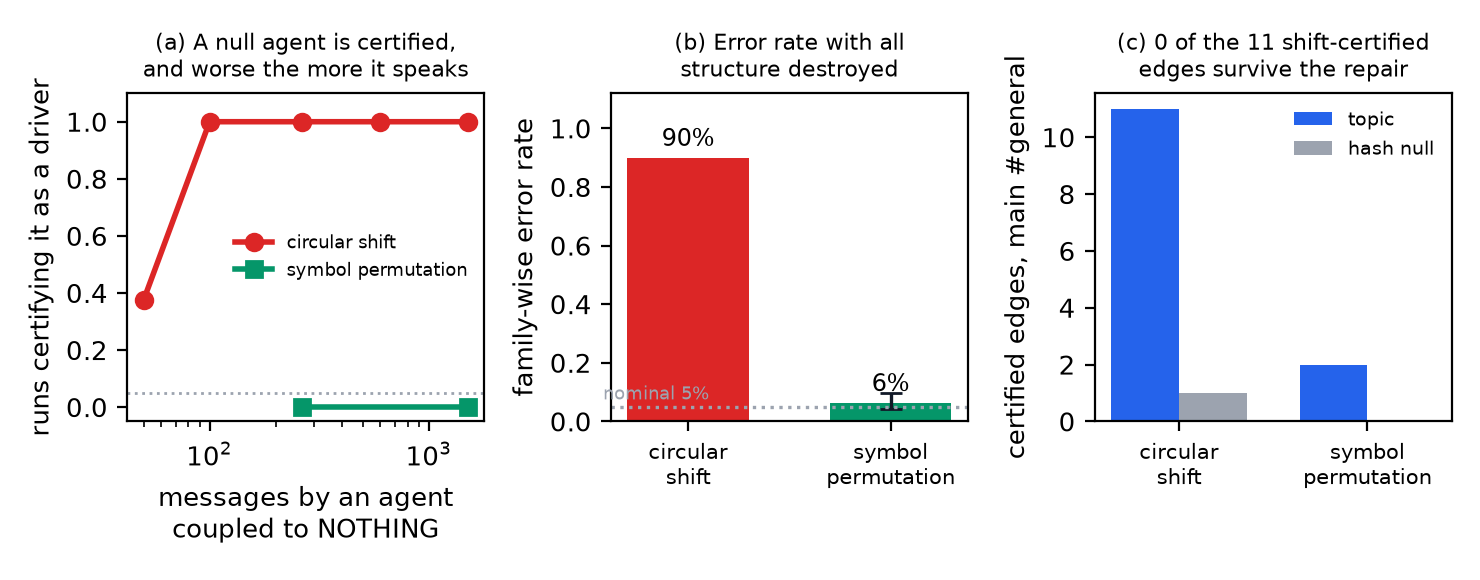
\includegraphics[width=\textwidth]{f2_null.png}
\caption{Left, how often an agent coupled to nothing is certified as a driver, under each surrogate.
Middle, family-wise error rate measured on data with all structure destroyed, with a Wilson
interval; the dotted line is the nominal 0.05. Right, what each surrogate certifies on the real
channel.}
\end{figure}

\subsection{How many surrogate draws are needed}

The number of surrogate draws matters more than I initially appreciated. In a paired comparison of
300 instances, where all four surrogates run on identical symbol grids so the outcomes are paired,
the global permutation surrogate produced a false-positive rate of 0.1167 with 100 draws, falling to
0.0700 with 200 draws, 95\% Wilson $[0.046, 0.105]$. This difference is statistically significant
(exact McNemar $p = 0.0043$). The block-local and Runge local permutations were less sensitive to the
increase: their corresponding rates changed from 0.0900 to 0.0767 and from 0.0967 to 0.0800.

At 200 draws, the global permutation's interval covers the nominal 0.05 and overlaps the real-data
estimate of 0.0633 $[0.0409, 0.0968]$. The real-data result is therefore corroborated rather than
overstated. For practical use, the important point is that reducing the number of surrogate draws
can materially change the result. In particular, the global permutation over-fires at 100 draws by
approximately a factor of two. I would therefore not treat the choice of draw count as a minor
computational detail.

The same correction applies to the benchmark-wide estimate. That figure was 0.0942 at 100 draws.
Repeating all 2,400 instances at 200 draws gives \textbf{0.0679}, 95\% Wilson $[0.0585, 0.0787]$,
and the paired difference is large: 83 instances fire at 100 draws and not at 200, against 20 the
other way, $p = 2.7 \times 10^{-10}$. The conclusion it supports is unchanged, because the interval
still excludes the nominal 0.05. So the permutation repair does carry a residual inflation on clean
generated data, but it is about a third above nominal rather than nearly double.

One limit on this recommendation. I compared 100 draws against 200 and did not test any larger
value, so what the experiment establishes is that 100 is too few, not that 200 is enough. Two
hundred is a lower bound on the draw count rather than a converged setting, and a practitioner whose
conclusions sit near a decision boundary should check their own sensitivity rather than adopt the
number.

\subsection{Choosing a repair, when the error rate cannot choose}

The comparison of the three permutation-based repairs does not produce a clear winner. All four
surrogates were evaluated on identical symbol grids across 300 pure-null replicates, so the
comparison reflects differences between the null models rather than differences between datasets.

\begin{table}[h]
\centering
\begin{tabular}{lrrrl}
\toprule
surrogate & FWER, 100 draws & FWER, 200 draws & 95\% Wilson at 200 & nominal 0.05 \\
\midrule
circular shift                   & 0.0433 & \textbf{0.0333} & $[0.018, 0.060]$ & inside \\
global within-speaker permutation & 0.1167 & \textbf{0.0700} & $[0.046, 0.105]$ & inside \\
block-local permutation          & 0.0900 & \textbf{0.0767} & $[0.052, 0.112]$ & excluded \\
local permutation \citep{runge2018} & 0.0967 & \textbf{0.0800} & $[0.054, 0.116]$ & excluded \\
\bottomrule
\end{tabular}
\caption{Four surrogates on identical symbol grids, 300 pure-null replicates, at both draw counts.}
\end{table}

At 200 draws, paired on the same 300 instances, the circular shift is not significantly different
from the global permutation ($p = 0.0614$), although it differs from block-local permutation
($p = 0.0294$) and from Runge's local permutation ($p = 0.0201$). At 100 draws it differed from all
three, which is the draw-count artifact again. The three repairs remain statistically
indistinguishable from one another, with pairwise $p$-values of 0.85, 0.65 and 1.00. The apparent
differences in their error rates are not sufficient to establish a ranking.

Choosing between them therefore requires more than calibration, and two readings pull against each
other. Runge's local permutation has the strongest methodological justification for preserving the
structure it is intended to preserve, and it follows the approach adapted to event data by
\citet{shorten2021}. Block-local permutation is more heuristic and introduces a free parameter that
has not been tuned. Global permutation is the simplest. On the other hand, the global permutation has
the most favourable interval relative to the nominal rate, and is the only repair that costs nothing
measurable against the shift on clean stationary data, although neither difference is statistically
established. I do not consider the observed error rates sufficient to select one repair over the
others. The choice should be guided by the structure the null is intended to preserve and the
assumptions that can be justified for the data.

\subsection{When to use the repair}

A drift sweep gives the practical reading. Across 150 replicates per cell at 200 surrogate draws,
the circular shift degrades steadily as activity drift increases while the three repairs do not.

\begin{table}[h]
\centering
\begin{tabular}{lrrrr}
\toprule
activity drift & circular shift & global permutation & block-local & local \\
\midrule
0.0 & \textbf{0.013} & 0.093 & 0.080 & 0.093 \\
0.3 & 0.100 & 0.100 & 0.093 & 0.120 \\
0.6 & \textbf{0.193} & 0.053 & 0.047 & 0.067 \\
0.9 & \textbf{0.380} & 0.087 & 0.080 & 0.080 \\
\bottomrule
\end{tabular}
\caption{Family-wise error on pure nulls as activity drift increases, 150 replicates per cell, 200
surrogate draws. Every certified edge is a false positive by construction.}
\end{table}

The pattern is supported by a formal trend test rather than by eye. A Cochran-Armitage test across
the four ordered drift levels gives the circular shift $z = 8.667$, $p < 10^{-15}$, and gives every
repair nothing: $p = 0.51$ for the global permutation, 0.63 for block-local and 0.37 for local. The
same pattern holds at both surrogate draw counts, so it does not depend on that choice.

The repairs are therefore flat under drift rather than calibrated. Only one of the four global
permutation intervals covers the nominal 0.05, and the rest sit nearer 0.09, so what the repair buys
is insensitivity to drift rather than correctness. One asymmetry should be stated rather than
hidden: block-local covers nominal in three of the four cells where the global repair covers one.
The two remain pairwise indistinguishable, so this is not grounds to switch the recommendation, but
it does mean the global repair cannot be described as the best-calibrated under drift.

The results also show why the repair should not be treated as universally preferable. At zero drift
the circular shift has an error rate of 0.013, while the three repairs are all around 0.08 to 0.09.
That advantage is gone by the first drift step: at drift 0.3 the shift reads 0.100 against the global
permutation's 0.100 and block-local's 0.093, so the crossover falls between drift 0.0 and 0.3 rather
than at some higher level. By drift 0.6 the shift is roughly four times the repairs. If a channel has
been checked and found stationary, the circular shift may be sufficient. When activity is
non-stationary the repairs are the more stable choice, and the margin for error on that judgement is
narrow, because the crossover arrives by the first drift level tested.

\section{Continuous time, and what the repair cannot test}

An earlier analysis identified continuous-time estimation as the principled option for event data
but did not evaluate it. Running the continuous-time estimator CoTETE on both channels certifies 0
edges in either case, compared with 2 for main-village and 18 for open-chat under the discrete,
turn-ordered analysis. Its highest $z$-scores are 3.062 and 3.980, below the respective max-T
thresholds of 4.171 and 4.308.

At first these results might appear to contradict the symbol-based analysis. The two estimators
operate on different information, however. CoTETE's public API takes event times with no symbol
channel, while the transfer-entropy analysis here uses topic symbols. To test whether this
difference explains the results, I reduced the data to timing alone, replacing every spoken symbol
with the same code. Under this representation the estimator used here also detects 0 edges in both
channels, matching CoTETE. Using the circular-shift surrogate instead produces 12 and 3 edges. So
neither method detects relationships from event timing alone in these channels, and the edges found
by the symbol-based analysis depend on symbol correspondence, which the continuous-time estimator
cannot access.

Two caveats attach to those $z$-scores, and the second attaches to the larger of them. Point
estimates from this estimator are stochastic to about 17\% across repeated runs, so none of these
values should be read to more than two significant figures. And open-chat's highest $z$, the 3.980,
belongs to the one pair whose surrogate draws mostly failed: it needed 1,936 failed draws to obtain
100 successes, a 4.9\% success rate. Those surrogates are conditioned on being estimable, so that
pair's null is biased in an unknown direction. The conclusion does not rest on it, since that pair
falls below threshold and so does every other pair, but the number should not be quoted as a clean
measurement. The failures themselves were a defect rather than a property of the data: an enlarged
exclusion window can empty the neighbour search on sparse bursty event trains and raise an error
that terminates a whole pair, with no handling at the public entry point. This has been reported
upstream.

There is also a fundamental limitation in applying the recommended permutation surrogate to
timing-only data. When every event carries the same symbol, permuting those symbols changes nothing.
The observed statistic and the surrogate null are identical, making the test exactly degenerate:
standard deviation 0 across all 210 pairs and $p = 1.0$ everywhere. \textbf{The repair has zero power
against timing structure by construction.} The permutation surrogate is appropriate for testing
relationships in the symbol sequence, but it does not answer whether relationships exist in event
timing. These are different questions, and choosing one null means giving up the ability to test the
other with that procedure.

\section{Confounding, and what conditioning removes}

A valid surrogate fixes calibration but not confounding. If every agent tracks a drifting channel
topic, every pair is genuinely dependent through the channel, and pairwise transfer entropy cannot
tell that from direct influence. I therefore also report a \textbf{conditional} estimate, which asks
whether a source's last message adds anything about a target's next one beyond the target's own
history and the channel's recent state. The conditioning variable is the modal symbol of the last
twelve messages, excluding the immediately preceding one so that it does not simply restate the
source.

On a generated benchmark whose decisive instances contain no influence while every agent tracks a
shared drifting topic, so that any certified edge is common cause, pairwise transfer entropy
certifies \textbf{22.3} edges on average and conditioning takes that to \textbf{0.33}, lifting pooled
precision on the four-edge instances from 0.17 to \textbf{0.80} at a recall of 1.0 either way. Across
couplings from 0.05 to 0.8 the conditional test still finds the planted edge in 3 of 3 runs, so the
gain costs no power.

The benchmark flatters the conditional estimator, since its common cause is a shared modal topic and
the conditioning variable is the channel's modal topic. The real channels are harder, and
conditioning there costs degrees of freedom: a 9-symbol alphabet with a 9-valued context gives 6,561
cells against about 7,900 ticks, so that variable is also coarsened to 4 and 2 values.

\begin{table}[h]
\centering
\begin{tabular}{lrrrr}
\toprule
channel & pairwise & conditional, 9 values & 4 values & 2 values \\
\midrule
main \#general      & 2  & \textbf{2, the same two edges} & 2 & 3 \\
open-chat \#general & 18 & \textbf{0} & \textbf{7} & \textbf{13} \\
swarm, room a       & 1  & \textbf{0} & & \\
\bottomrule
\end{tabular}
\caption{Conditioning at three resolutions. Main-village's two edges are robust to that choice;
open-chat's zero is not.}
\end{table}

At the finest resolution the open-chat test is degenerate, its surrogate sitting above the observed
statistic for 65\% of pairs with the largest $z$ in the family only 4.4, so it is failing to reject
rather than finding nothing to reject. Open-chat's structure therefore remains
\textbf{undetermined}: depending on the conditioning resolution, between 0 and 13 of its 18 edges may
survive. That resolution is a free parameter an analyst would set once and never revisit. This is a
property of the channel rather than the estimator: on structure-free real data the conditional test
fires in 2 of 40 replicates, an error rate of 0.05 with a mean $z$ of $-0.001$, so it is nominal
rather than conservative.

\section{The symbolisation floor}
\label{sec:floor}

Everything these methods produce is downstream of turning text into symbols. On the benchmark, where
the underlying topics are known, detection performance drops sharply when agreement between the
symboliser and the ground truth falls below roughly ARI 0.44, and this behaviour appears across the
tested estimators. Importantly, the false-positive rate can look \emph{better} below this point,
because the shared topic structure needed to produce confounded detections is no longer represented
reliably. A pipeline that stops detecting relationships may therefore have lost the signal it needs
rather than become more reliable, and nothing downstream of the symboliser can tell those apart.

\subsection{Detecting the floor without labels}

That degradation can be detected without ground-truth labels. Across the nine-level benchmark sweep,
three statistics separate the below-floor cases with zero errors: seed stability at a threshold of
0.623, agreement with LSA at 0.646, and the Calinski-Harabasz index at 138.9. Seed stability here is
the \textbf{minimum} pairwise agreement across seeds, not the mean; the mean variant makes one error,
at a different threshold of 0.791. Silhouette has the strongest correlation with true ARI, at 0.979,
but is not useful for identifying the boundary because its threshold falls within a gap of just
0.002. A statistic that tracks clustering quality most closely is not necessarily the best one for
making a classification decision.

Error count cannot choose among the three that were perfect, so I tested whether each threshold still
means what it meant when the channel changes for reasons other than topic separability. Applying each
cut unchanged to thirty cells that vary turn-taking, drift, agent count, volume skew, message length
and corpus size, twenty-seven of which hold true ARI at exactly 1.000:

\begin{table}[h]
\centering
\begin{tabular}{lrrrr}
\toprule
diagnostic & cut & errors where fitted & errors, nuisance set & of those at true ARI 1.000 \\
\midrule
seed stability, min across seeds & 0.623 & 0 & 2 & \textbf{0} \\
LSA agreement                    & 0.646 & 0 & 2 & \textbf{0} \\
Calinski-Harabasz                & 138.9 & 0 & 6 & \textbf{3} \\
\bottomrule
\end{tabular}
\caption{Whether a cut fitted on the vocabulary-overlap mechanism survives a change in the channel
that is not a change in topic separability.}
\end{table}

The two bounded statistics err only on the short-message cells, where the symbolisation genuinely has
degraded. Calinski-Harabasz additionally condemns all three cells whose true ARI is exactly 1.000,
for no reason beyond the corpus holding 2,000 messages rather than 8,000, where it reads 76 to 77
against its own cut of 138.9. It is unbounded and grows with sample size, so a published numeric
threshold for it carries no meaning on another corpus. That is why I recommend the two bounded
statistics and not the index that matched them on error count. \textbf{A cut that moves with the
corpus is not a floor cut.}

This is not a weak statistic being discarded on a technicality. Calinski-Harabasz correlates with
true ARI at 0.973, almost as closely as silhouette, and unlike silhouette it classifies the floor
perfectly where it was fitted. It still cannot carry a published threshold. That is the sharper form
of the point above: neither the statistic that tracks quality most closely nor the one that
classifies best on the fitting mechanism is necessarily the one whose cut another researcher can
reuse.

There are important limits to this result. The effective sample size is nine rather than 54, because
the classification label is determined by overlap level. There are no observations between ARI 0.444
and 0.222, so the exact location of the boundary within that interval remains unknown. These
diagnostics classify whether a result is below the tested detection floor; they do not estimate ARI,
and their behaviour is flat between 0.68 and 1.00, and not even monotone there. The benchmark also
uses a single degradation mechanism with a known and correct value of $k$, whereas the true number of
topics in real conversations is unknown. I therefore treat 0.44 as a benchmark-specific, bracketed
result rather than a universal threshold.

\subsection{A contradiction the diagnostic lost}

I initially used these diagnostics to classify one real channel, open-chat, as below the
symbolisation floor. That conclusion did not agree with the channel's measured results: open-chat
certified 18 and 22 edges under the two symbolisers, compared with 2 and 1 for main-village, and its
hash-based null certified zero edges. Rather than treating this disagreement as evidence that the
original measurements were wrong, I revisited the diagnostic itself.

The problem was the choice of $k$. Repeating the comparison with the same channels, loader and window
reproduced the published $k=8$ results to the digit. At $k=4$, however, open-chat reached stability
scores of 0.950 and 0.978, the highest values produced by either channel across the tested settings,
and both exceeded the diagnostic thresholds. The earlier below-floor classification was therefore a
conclusion about one arbitrary choice of $k$, not a reliable statement about the channel. Message
length does not explain the difference either: 27.1\% of main-village messages contain fewer than
five tokens, compared with 2.3\% in open-chat, so the short-message channel is the one the diagnostic
cleared.

This correction changes how the symbolisation results should be read, and it withdrew three claims.

\begin{enumerate}
\item \textbf{The claim that no topic signal remains below the floor is too strong.} The
circular-shift surrogate recovers all four planted edges at every tested overlap level, including
0.95, where ARI is 0.011. The observed collapse is in the permutation null, not necessarily in the
underlying data.
\item \textbf{ARI 0.44 cannot be treated as a universal detection threshold.} When the shared-topic
parameter is 0, detection continues down to ARI 0.296, so the boundary depends on both the
symboliser and the channel.
\item \textbf{Edge counts cannot be used as a measure of symboliser quality.} Even at ARI exactly
1.000, changing the shared-topic parameter alone moves the permutation edge count from 5 to 78.
\end{enumerate}

The diagnostics also do not transfer reliably outside the mechanism on which they were evaluated.
Their balanced accuracy falls from 1.00 to 0.75 and 0.571 under a known mismatch in $k$. All seven
errors made by seed stability are false below-floor classifications, and in every one of those cases
the detector still identifies all planted edges; of the fourteen cells it condemned, eleven had full
conditional recall. The failure direction is the dangerous one: it condemns working symbolisations.

This was an important correction to my own interpretation. I introduced a diagnostic to check whether
the symbolisation was reliable, applied it to the real channels, and found that it contradicted
measurements already in hand. Investigating that contradiction showed the diagnostic was sensitive to
an arbitrary modelling choice. The result is not that the original measurements were wrong, but that
the control was being asked to support a broader conclusion than the evidence allowed. These
diagnostics remain useful within their tested setting, and \textbf{no channel-level floor verdict
should be issued from a single $k$}.

\section{The benchmark}

Real logs have no ground truth, so the common-cause question could not be settled on them. The
generator used here makes the influence graph known by construction: it decides, in code, who speaks
at which tick, on which topic, and who reacts to whom. Surface text is a separate, replaceable layer
drawn from disjoint per-topic vocabularies, so the whole thing runs offline and a detector still has
to symbolise raw text rather than read the labels. Turn-taking and activity drift are independent
knobs, so the two can be varied one at a time, and the generator reproduces its earlier behaviour
bit for bit when both are zero.

\benchname{} is released with 150 tests covering the generator, the detector harness, the text layer,
the floor analysis and the turn-taking factorial.
\ifdeanon{Code and benchmark:
\url{https://github.com/manunicholasjacob/swarm-influence-bench} and
\url{https://github.com/manunicholasjacob/swarm-influence-audit}.}{Code and benchmark are publicly
released; the links are withheld here for anonymity and will be given in the camera-ready version.}

One property of the benchmark must be stated when its numbers are quoted. Planting an edge displaces
other agents' speaking turns, so the generated instances contain real lag-1 dependencies that the
label set does not list. Precision measured against those labels is therefore a \textbf{lower bound}
for any detector, and what the benchmark supports is the comparison between two estimators rather
than the absolute value of either.

\section{What an overseer should do}

Six inexpensive controls should be included whenever an influence graph over an agent channel is
published.

\begin{enumerate}
\item \textbf{Plant an agent coupled to nothing, at your channel's volumes, and check it is not
certified.} This one test would have caught the failure reported here, at one run per volume.
\item \textbf{Measure the error rate directly}, by destroying the structure your method claims to
find and checking the family-wise rate is near nominal. If it is not, your surrogate does not match
your data.
\item \textbf{Preserve the speaker sequence in your surrogate.} Any surrogate that moves an agent's
messages in time will disturb it, and \citet{shorten2021} is the principled route. Use at least 200
surrogate draws, because at 100 the global within-speaker permutation over-fires by roughly a factor
of two.
\item \textbf{Establish the detection floor before interpreting an absence.} ``No edges'' and ``no
influence'' are different claims.
\item \textbf{Condition on the channel, report both numbers, and sweep the resolution.} Pairwise and
conditional bound the answer, and the gap between them is the result. Conditioning costs cells, so
check whether your answer is an artifact of how finely you conditioned. On one channel here it was.
\item \textbf{Report how well your symboliser agrees with the truth, on data where you know it.}
Everything is downstream of turning text into symbols, and below roughly ARI 0.44 detection
collapses whatever the estimator. I have found this control in no influence-detection paper, and it
is also the one that cannot be run on real logs, which is why the floor remains the largest
unquantified threat here.
\end{enumerate}

Two habits follow: publish a meaning-free null's count beside the real one, and require held-out
replication before calling a graph a structure.

\section{The real channels, and what survives}

Re-running every channel under the repaired surrogate changes the answers, and not in one direction.

\begin{table}[h]
\centering
\begin{tabular}{lrrr}
\toprule
channel & window messages & shift: topic / hash & permutation: topic / hash \\
\midrule
main \#general      & 8,800 & 11 / 1 & 2 / 0 \\
open-chat \#general & 8,226 & 3 / 0  & 18 / 0 \\
swarm, room a       & 3,846 & 2 / 1  & 1 / 0 \\
\bottomrule
\end{tabular}
\caption{The same channels under both surrogates, with the meaning-free hash null beside each.}
\end{table}

In main-village, \textbf{none} of the 11 edges the standard recipe certifies survives the repair, and
the two the valid surrogate certifies were not among them. In open-chat the correction runs the other
way, 3 edges becoming 18, because pathological pairs inflate the max-T threshold and raise the bar
for everything else. An invalid surrogate does not simply add false positives; it scrambles the
result.

Main-village's two edges are the strongest thing here and they are still not a finding, because they
do not replicate: the adjacent fourteen-day window certifies nothing at all under either estimator.
Given the detection floor, that silence is as consistent with the test sitting near its limit as with
the edges being absent, and the two cannot be separated. Power is governed by how much an agent says
as much as by how strongly it copies, and it is channel-specific: in main-village a planted follower
copying on 80\% of its messages is caught only 1 time in 4, while in open-chat one copying 10\% of
the time is caught 3 times in 4. Replication is weak everywhere: under the standard recipe the
adjacent window shares 1 edge out of 8 and 4, and that edge is also the only one the hash null
certifies. No certified edge in this work replicates out of sample.

\begin{figure}[h]
\centering
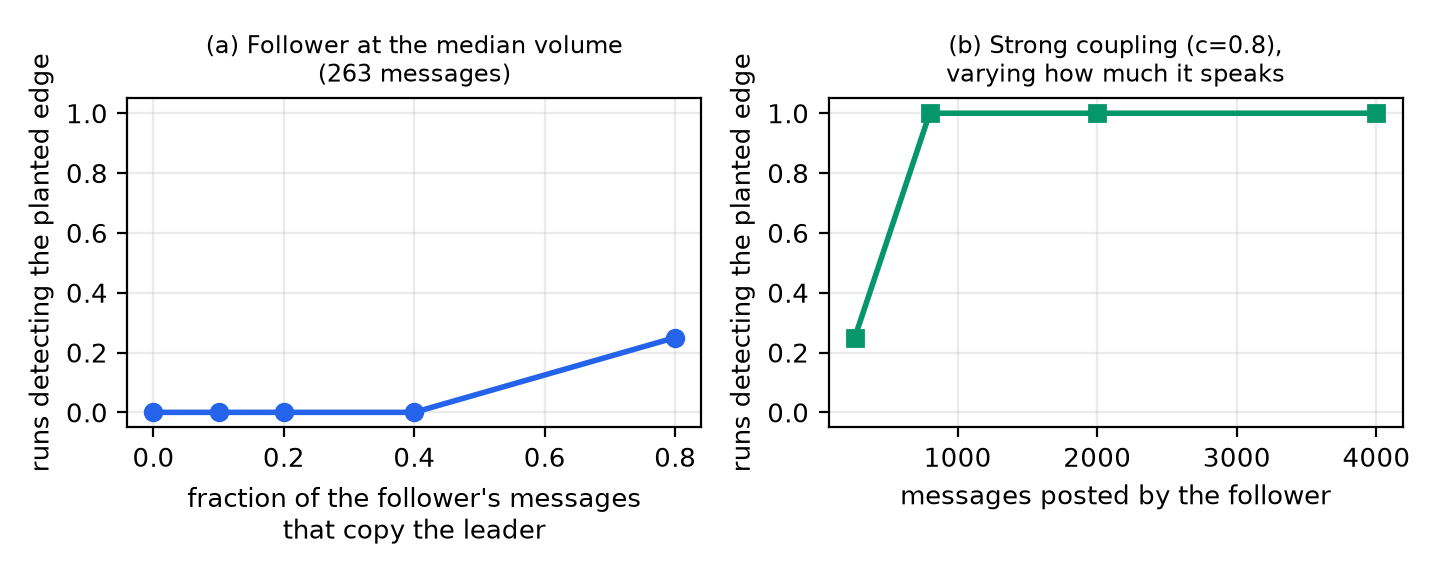
\includegraphics[width=0.92\textwidth]{f4_power.png}
\caption{Detection of a planted follower under the repaired surrogate. Left, varying the fraction of
its messages that copy the leader, at the median agent's volume. Right, varying how much it speaks,
at strong coupling.}
\end{figure}

\paragraph{Humans in the channel.} Main-village \#general is now effectively human-free, with 3 human
messages in the window, so the question has to be asked in open-chat, where 32\% of messages come
from 124 human visitors. Pairwise, with humans collapsed into one node, 19 edges are certified.
Conditioning removes almost all the agent-to-agent structure and little of the rest: \textbf{four
edges survive, of which three run from humans to agents, one is agent to agent, and none run from an
agent to a human.} The asymmetry is not an artifact of the confound. It should be read carefully all
the same: topical dependence from a person to an agent is also what ordinary responsiveness looks
like, so the measurement supports only that the dependence is dyad-specific and directional, not
that anyone is steering a swarm.

\section{Reproducibility, and one limitation of it}

Every number in this paper is recomputed from committed analysis output by a verifier that fails on a
mismatch, and that verifier covers the prose of this paper as well as the figures.

One limitation should be stated plainly. Re-running the counts in the earlier stationarity sweep with
the same seeds and configuration, only one of the eight cells reproduced exactly; the remaining
differences were one or two replicates per cell. Seven of the eight published rates still fell within
the recomputed Wilson intervals, and no conclusion changed. The exception is the zero-drift cell under
the permutation null, where the published 1 of 30 falls just below the recomputed interval of
$[0.035, 0.256]$ for 3 of 30, and no result here depends on that cell.

The generator, estimator and BLAS configuration were investigated and ruled out as the source. The
most likely explanation is a library-level difference, particularly in scikit-learn's $k$-means
implementation within the symboliser, whose output can vary between versions. Every sweep now records
the environment it ran under: Python 3.14.6, numpy 2.5.1, scipy 1.18.0 and scikit-learn 1.9.0,
including the BLAS build and the number of BLAS threads each worker used.

This does not make the previously published counts exactly reproducible. It provides a more clearly
specified environment in which subsequent results can be checked. For that reason I report rates
alongside their confidence intervals rather than exact replicate counts. The distinction between
reproducing a result within its uncertainty and reproducing every individual count matters, and only
the first is claimed.

\section{Conclusion}

Applied to real agent chat, the standard recipe for ``who drives whom'' needs repair before it says
anything. Clock windows cannot separate a message from its answer at the speed agents reply, and what
they certify is matched by a null with no access to meaning. The turn-ordered grid that fixes this
breaks the circular-shift surrogate: family-wise error 0.90 against a nominal 0.05, caused by the
speaker sequence itself. Restricted permutation surrogates repair most of that, but they are flat
under drift rather than calibrated, they are mutually indistinguishable at this precision, and one of
them needs twice the surrogate draws anyone would think to use. A valid surrogate fixes calibration
but not confounding. What survives is small: two dyad-specific edges that do not replicate, an
undetermined answer set by conditioning resolution, and influence running from people into agents and
never back. \textbf{An influence graph should not guide decisions until its error rate, its confound,
its detection floor and its symboliser's fidelity are reported.}

\section*{Limitations}

\begin{itemize}
\item \textbf{Immediate-predecessor only.} The turn-ordered lag-1 measure sees influence from the
message directly before a reply. Influence acting over several turns, or through a room's accumulated
context, is out of scope.
\item \textbf{Discrete approximation to an event process.} Agent chat is event-based in continuous
time. The turn-ordered discretisation with a permutation surrogate is a practical fix, and the
continuous-time comparison above shows what that choice gives up.
\item \textbf{The mechanism behind the real 0.90 is not established.} The generator separates
turn-taking from drift and points at drift, but the largest cell anywhere in the design is 0.365.
\item \textbf{Symbolisation quality cannot be measured on the real logs.} The central result survives
an independent symboliser, but the edge count does not: it moves with alphabet size and with which
messages the topic model is fit on. The floor remains the largest unquantified threat.
\item \textbf{No ground truth in the real logs.} The validity argument rests on planted controls and
on the meaning-free null, not on recovering a known answer.
\item \textbf{Conditioning removes real influence too.} The conditional estimate discards influence
that works by shifting what the channel is talking about, which in a group chat may be a large part
of genuine influence. It is a lower bound on dyadic influence.
\item \textbf{The human result is exploratory.} It rests on one village and one window and should be
read as a lead.
\end{itemize}

\section*{Broader impact and ethics}

This work audits influence detection on a population of AI agents, which is dual-use. Used
defensively it helps an overseer decide what an influence graph is worth, and the main result is
deflationary: it tells practitioners to trust these outputs less, which reduces rather than increases
the chance of acting on a bad attribution. The same tooling could be used to identify the most
influential agent in a swarm in order to target it, or to surveil participants in a channel. Three
properties limit the misuse. The subjects are AI models; the dataset is already public under research
terms and no re-identification is added; and the measure is weak and local, recovering
immediate-predecessor topical dependence rather than any model of how to steer an agent.

The dataset's research terms were followed: research use only, no training on the data, no
re-identification, citation of the source, and notification of the authors of resulting publications.
Human participants appear only as an aggregate node or as anonymised visitor labels, never by name or
handle, and no content attributable to an individual person is reported. Message text and metadata
were read, never model weights or private user data.

The use of a large language model in this work is disclosed in the first-page footnote, as TMLR
requires.

\bibliographystyle{tmlr}
\bibliography{refs}

\end{document}
